\chapter{Realization of the direct T symmetry test at KLOE}\label{chapter:analysis_kloe}

The direct test on the symmetry under reversal in time at KLOE described in~\cref{chapter:test_kloe} requires mutual comparison of time-dependent rates of four classes of processes~(listed in~\tref{tab:processes}), each characterized by specific decays of both neutral K mesons present in a $\phi\to\Ks\Kl$ event. In a practical data analysis at KLOE, it is reasonable to limit the study to using semileptonic decays with electrons and positrons rather than muons and in case of decays into two pions, to choose $\pi^+\pi^-$ rather than $\pi^0\pi^0$ as the two-pion state due to good reconstruction of the former in the drift chamber. Moreover, it can be noted that the processes indicated in~\tref{tab:processes} comprise two general classes, each of which is additionally split into two categories by charge of the lepton in the semileptonic decay. These two classes, presented schematically in~\fref{fig:event_schemes}, are:

\begin{enumerate}
\item events with an earlier kaon decay into a semileptonic final state $\pi^-e^+\nu_e$ or $\pi^+e^-\bar{\nu}_e$, characterized by two tracks recorded in the DC and with an unregistered neutrino, and a later kaon decay into $3\pi^0$ resulting in up to 6 points of $\gamma$ quanta interaction in the EMC~(\fref{fig:event_schemes:a}),
\item events with an earlier neutral kaon decay into two charged pions, characterized by two DC tracks originating close to the $\phi$ decay point, and a later semileptonic decay into $\pi^-e^+\nu_e$ or $\pi^+e^-\bar{\nu}_e$ recorded as two tracks with a common origin anywhere in the drift chamber volume, where the neutrino escapes detection~(\fref{fig:event_schemes:b}).
\end{enumerate}

\begin{figure}[h!]
  \centering
  \begin{subfigure}{0.45\textwidth}
  \begin{tikzpicture}[scale=0.45,
  font={\fontsize{14pt}{12}\selectfont}
  ]
  \coordinate (kldec) at (4.0,2);
  \coordinate (ksdec) at (-1,-0.33);
  \draw[gray!60, line width=8] (0,0) circle (7.0);
  
  \draw[line width=1,densely dotted] (0,0) -- (kldec);% node[black,midway,above]{$\kaon$};    
  \draw[line width=1,densely dotted] (0,0) -- (ksdec);% node[black,midway,above]{$\kaon$};    

  % clusters
  \draw[black!85,fill] (100:7) circle (0.2);
  \draw[black!85,fill] (70:7) circle (0.2);
  \draw[black!85,fill] (40:7) circle (0.2);
  \draw[black!85,fill] (10:7) circle (0.2);
  \draw[black!85,fill] (-15:7) circle (0.2);
  \draw[black!85,fill] (-50:7) circle (0.2);

  \draw[black!85,fill] (173:7) circle (0.2);
  \draw[black!85,fill] (-122:7) circle (0.2);
  
  \draw[arrows={-{Triangle}[width=5,length=6]},thick, dashed] (kldec) -- (100:6.85) node[midway, left, xshift=-8] {$\gamma$};
  \draw[arrows={-{Triangle}[width=5,length=6]},thick, dashed] (kldec) -- (70:6.85) node[midway, left] {$\gamma$};
  \draw[arrows={-{Triangle}[width=5,length=6]},thick, dashed] (kldec) -- (40:6.85) node[midway, left, yshift=8,xshift=5] {$\gamma$};
  \draw[arrows={-{Triangle}[width=5,length=6]},thick, dashed] (kldec) -- (10:6.85) node[midway, left, yshift=6,xshift=12] {$\gamma$};
  \draw[arrows={-{Triangle}[width=5,length=6]},thick, dashed] (kldec) -- (-15:6.85) node[midway, left, yshift=-15,xshift=8] {$\gamma$};
  \draw[arrows={-{Triangle}[width=5,length=6]},thick, dashed] (kldec) -- (-50:6.85) node[midway, left] {$\gamma$};

  
  \draw[arrows={-{Triangle}[width=5,length=6]}] (ksdec) arc (30:125:4) node[midway,above]{$e^\pm$};
  \draw[arrows={-{Triangle}[width=5,length=6]}] (ksdec) arc (360:308:7) node[midway,left]{$\pi^\mp$};
  \draw[dashed, arrows={-{Triangle}[width=5,length=6]}] (ksdec) -- (-7, -5.5) node[midway, above]{$\nu$};

  % decay dots
  \draw[darkgray,fill] (0,0) circle (0.1) node[black,below]{$\phi$};
  \draw[darkgray,fill] (ksdec) circle (0.1);
  \draw[darkgray,fill] (kldec) circle (0.1);
\end{tikzpicture}        
\caption{$\Ks \Kl \to \pi^{\pm}e^{\mp}\nu 3\pi^0$ event.}\label{fig:event_schemes:a}
\end{subfigure}
\hspace{1em}
\begin{subfigure}{0.45\textwidth}
\begin{tikzpicture}[scale=0.45,
  font={\fontsize{14pt}{12}\selectfont}
  ]
  \coordinate (kldec) at (4.0,2);
  \coordinate (ksdec) at (-1,-0.33);
  \draw[gray!60, line width=8] (0,0) circle (7.0);

  \draw[line width=1,densely dotted] (0,0) -- (kldec);% node[black,midway,above]{$\kaon$};    
  \draw[line width=1,densely dotted] (0,0) -- (ksdec);% node[black,midway,above]{$\kaon$};    
  
  % ks decay
  \draw[black!85,fill] (166:7) circle (0.2);
  \draw[arrows={-{Triangle}[width=5,length=6]}] (ksdec) arc (40:100:6) node[midway,above]{$\pi^\pm$};a
  \draw[black!85,fill] (242:7) circle (0.2);
  \draw[arrows={-{Triangle}[width=5,length=6]}] (ksdec) arc (10:-52:6) node[midway,left]{$\pi^\mp$};

  % kl decay
  \draw[black!85,fill] (44:7) circle (0.2);
  \draw[arrows={-{Triangle}[width=5,length=6]}] (kldec) arc (190:132:3) node[midway,left]{$e^\pm$};a
  \draw[black!85,fill] (9:7) circle (0.2);
  \draw[arrows={-{Triangle}[width=5,length=6]}] (kldec) arc (230:273:4) node[midway,below]{$\pi^\mp$};
  \draw[dashed, arrows={-{Triangle}[width=5,length=6]}] (kldec) -- (20:8.5) node[midway, above]{$\nu$};  

  % decay dots
  \draw[darkgray,fill] (0,0) circle (0.1) node[black, below]{$\phi$};
  \draw[darkgray,fill] (ksdec) circle (0.1);
  \draw[darkgray,fill] (kldec) circle (0.1);
\end{tikzpicture}
\caption{$\Ks \Kl \to \pi^{+}\pi^{-} \pi^{\pm}e^{\mp}\nu$ event.}\label{fig:event_schemes:b}
\end{subfigure}
\caption{Schemes of the two processes studied in KLOE for the direct T symmetry test. Dotted lines represent paths travelled by neutral kaons before their decays and dashed lines denote photons and neutrinos, both invisible for the detector DC. Tracks of charged particles recorded by the DC are marked with solid lines. Black circles denote energy deposition clusters in the EMC barrel (grey band).}\label{fig:event_schemes}
\end{figure}

Although these sequences of final states can in principle originate from any order of $\Ks$ and $\Kl$ decays, due to the suppression of \CPs-violating decay modes $\Ks\to 3\pi^0$%
\footnote{The $\Ks\to 3\pi^0$ decay has, in fact, never been observed~\cite{Babusci:2013tr}.}
and $\Kl\to\pi^+\pi^-$~(see~\tref{tab:kaon_properties}) the earlier decays are expected to come from short-lived kaons in the regime of large time differences between both kaon decays which is under study in this work (see~\sref{sec:strategies}). As a result, the final state $\pi^{\mp}e^{\pm}\nu$ in the first class of processes and $\pi^+\pi^-$ in the second one originate close to the $\phi$ decay point defined by $e^+e^-$ collisions, with a distance corresponding to several times the mean free path of $\Ks$ at KLOE, $\lambda_S\approx 6$~mm. On the other hand, the second decay in each class may originate anywhere in the detector volume.

In the analysis presented in this work, the data collected by the KLOE experiment in the years 2004-5 were explored, with a total integrated luminosity of about~1.7~fb$^{-1}$. Performance of each of the analysis steps was evaluated using a sample of Monte Carlo (MC) simulated events corresponding to the conditions and integrated luminosity of the experimental data and including simulation of the full detector response~\cite{data_handling}. As mentioned in~\sref{sec:streaming}, the data of KLOE is pre-sorted into several streams and in this work the selection of relevant event classes was started from the 
% MEMO TODO: napisac explicite ze KSL
neutral kaon stream. The same streaming selection was applied to the data and MC samples used.

This Chapter presents details of event selection and reconstruction for the two aforementioned classes of processes, respectively in Sections~\ref{sec:t-analysis-1} and~\ref{sec:t-analysis-2}.
The direct \Ts~symmetry test imposes two crucial requirements on its experimental realization. Firstly, the samples of events of interest must be selected from all processes recorded by KLOE with a high purity as any background contamination will have a direct impact on the sensitivity of the test. From the branching ratios contained in~\tref{tab:kaon_properties} is is apparent that achieving the desired purity is the most challenging task in case of the $\Ks\to \pi^{\mp}e^{\pm}\nu$ decay as its probability is only at the level of $10^{-4}$. Therefore its selection comprises, in addition to a set of cuts based on the signal properties~(\sref{sec:ksemil}), also two steps dedicated to removing particular background components described in Sections~\ref{sec:ks2pi0_rejection} and~\ref{sec:pimu_rejection}. The second requirement of this analysis is that the time differences between two kaon decays, and thus also the decay times, must be reconstructed with a precision sufficient to study the double decay rates as functions of $\Delta t$~(see~\sref{sec:observables}). Whereas for all the involved decays which include charged particles, the decay times are easily obtained with an accuracy at the level of~1~$\tau_S$, the $\Kl\to 3\pi^0$ process requires special treatment to this end. With its reconstruction limited by the resolution of the calorimeter (inferior to the DC vertexing), a special kinematic fit is introduced to enhance time resolution for this decay (\sref{sec:kinfit}).

\section{Selection and reconstruction of the $\Ks \Kl \to \pi^{\pm}e^{\mp}\nu 3\pi^0$ process}\label{sec:t-analysis-1}

\subsection{Preselection of events}\label{sec:preselection-t1}
In order to properly reconstruct the decay time $\Delta t$ in a $\Ks \Kl \to \pi^{\pm}e^{\mp}\nu 3\pi^0$ event, decay vertices of both kaons must be available. Therefore, the first requirements imposed on events from the neutral kaon stream comprise (compare~\fref{fig:event_schemes:a}):
\begin{itemize}
\item presence of a vertex constituted by two approaching DC tracks in a cylindrical volume close to the $e^+e^-$ collision point limited by~$r_T=\sqrt{x^2+y^2}<$15~cm and $|z|<$10~cm,
% MEMO TODO: dopisac, ze wymagany qualv
\item presence of at least~6 EMC clusters not associated to DC tracks and with deposited energies $E>20$ MeV.
\end{itemize}
The volume for the 2-track vertex location is broad enough to contain almost all $\Ks$ decays~\cite{daria_memo, daria_article}. For the second requirement, track-to-cluster associations are determined by identifying sets of tracks corresponding to decay chains and extrapolating last track in each chain to the calorimeter inner surface. An EMC cluster is considered as associated to a track if distance between its centroid and the point of track incidence on EMC, measured in a plane perpendicular to the direction of incidence, is closer than 30~cm~\cite{data_handling}. Clusters associated to DC tracks constitute candidates for interaction points of charged particles which reached the EMC (e.g.\ all the clusters in~\fref{fig:event_schemes:b}), therefore only those without track association are considered for the identification of $\Kl\to 3\pi^0\to 6\gamma$. \fref{fig:t1-early-cuts} (left) shows the distribution of energy for all clusters with no associated tracks and for those originating from $\Kl\to 3\pi^0$ (signal) according to MC simulations. The dip below 20~MeV in the signal spectrum corresponds to the EMC threshold for efficient registration of $\gamma$~quanta while the peak for lower energies arises from effects such as cluster splitting in which one particle interaction is recorded by the calorimeter as several clusters.
% TODO: cytowac splitting
% TODO: sprawdzic czy to prawda
A cut on $E>$20~MeV thus allows to discriminate a large part of background clusters as well as reject poorly reconstructed events.

\begin{figure}[h!]
  \centering
  \begin{tikzpicture}
    \node[anchor=south west,inner sep=0] at (0,0) 
    {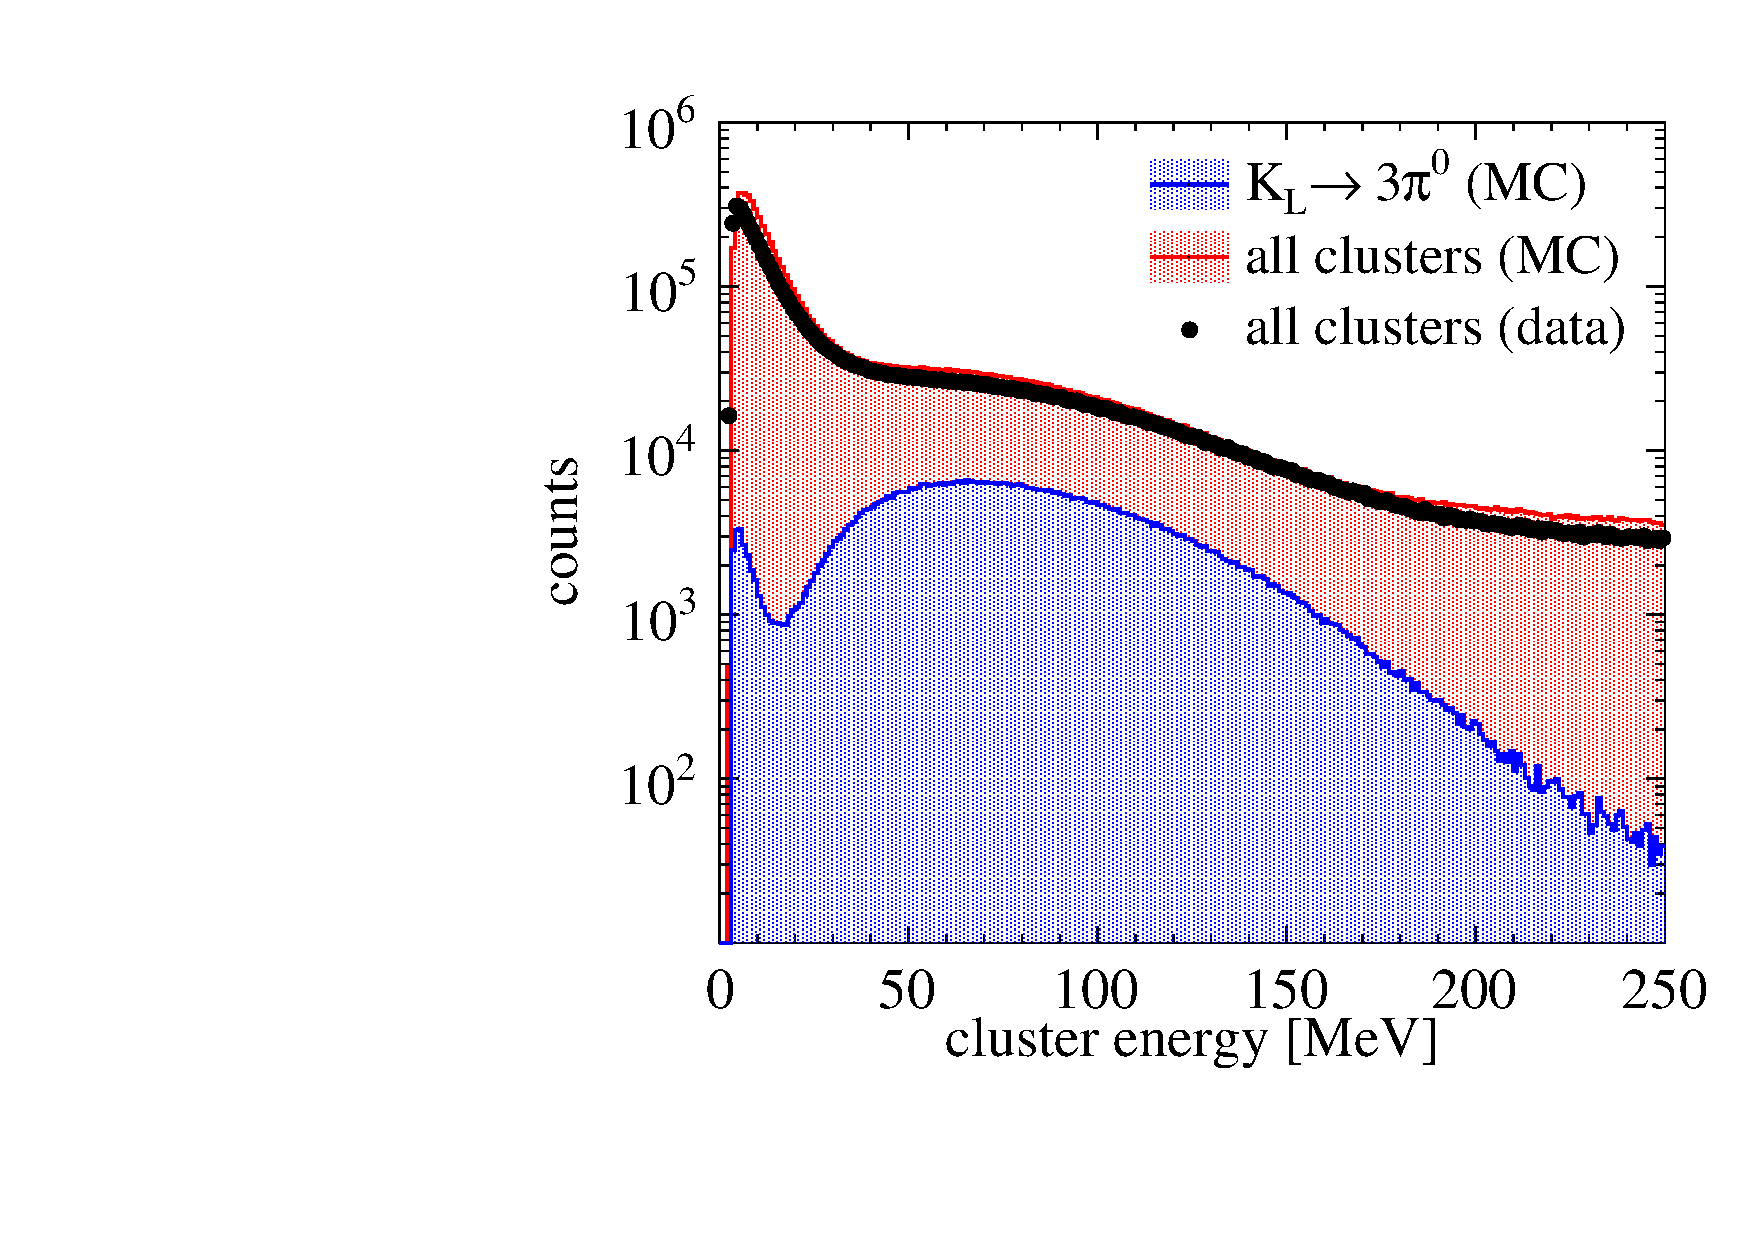
\includegraphics[width=0.45\textwidth]{Chapter7_analysis_kloe/img/cluster_energy_3pi0_v2}};
    \draw[black, thick, dashed] (1.52,0.8) -- (1.52,5.46);
    \draw[ultra thick, black!70!white, ->] (1.57, 5) -- (2.2, 5);
  \end{tikzpicture}
  \hspace{1em}
  \begin{tikzpicture}
    \node[anchor=south west,inner sep=0] at (0,0) 
    {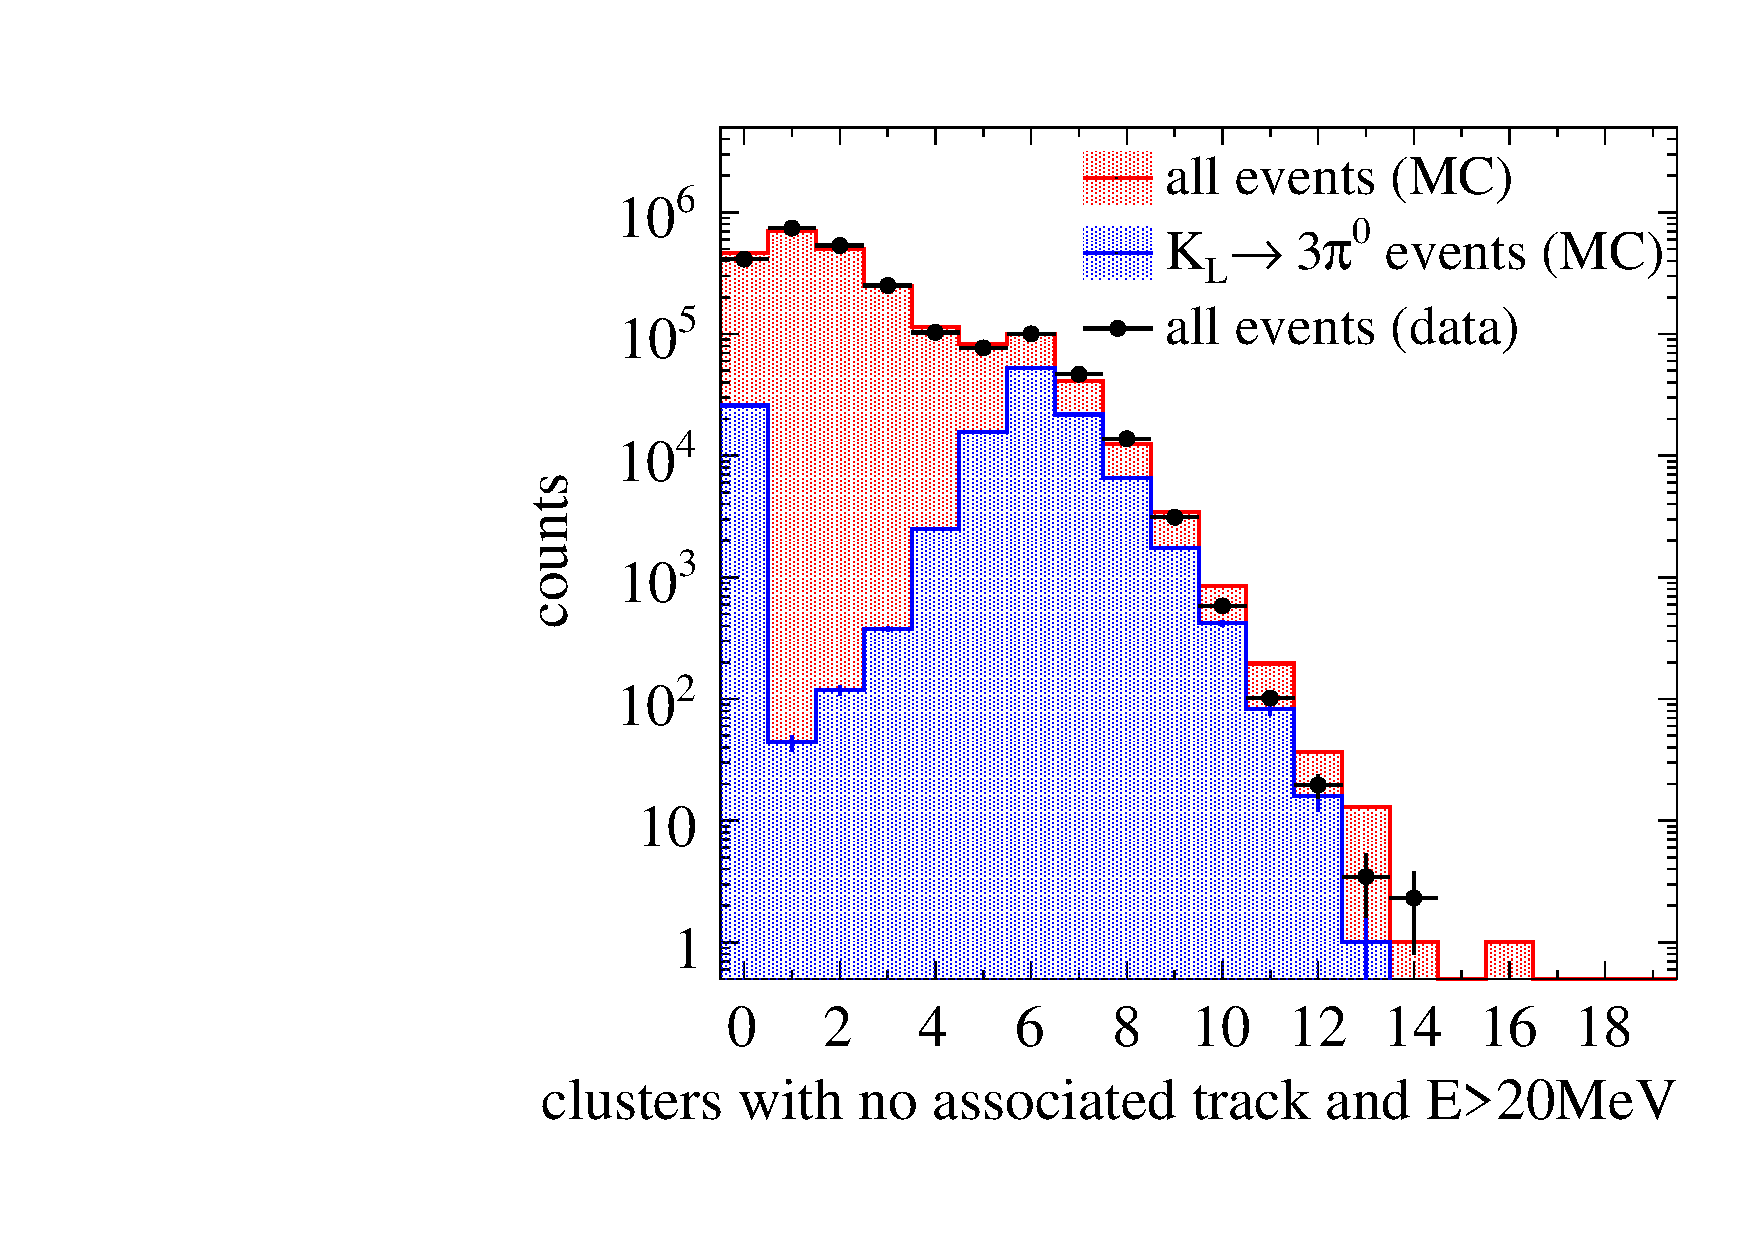
\includegraphics[width=0.45\textwidth]{Chapter7_analysis_kloe/img/no_neutral_clusters_v2}};
    % \draw[very thin,step=0.2] (0,0) grid +(5.5,5.5);
    % \draw[very thin,step=0.2] (0,0) grid +(5.5,5.5);
    \draw[black, thick, dashed] (2.73,0.8) -- (2.73,5.46);
    \draw[ultra thick, black!70!white, ->] (2.78, 1.5) -- (3.3, 1.5);
  \end{tikzpicture}
  \caption{Left: energy distributions of clusters not associated to DC tracks. Dashed line denotes minimum required energy.
    %for all clusters recorded in any events in the neutral kaon stream (red) and for clusters originating from $\Kl\to 3\pi^0 \to 6 \gamma$ (blue) as well as all data (black points).
    Right: numbers of $E>20$~MeV clusters not associated to DC tracks in a single event. Events with at least 6 such clusters are accepted as marked with the dashed line and gray arrow.
    % present in all MC events (red) and MC events containing a $\Kl\to 3\pi^0$ decay (blue) as well as data (black points).
  }
  \label{fig:t1-early-cuts}
\end{figure}

The distribution of the number of clusters with sufficient energy in a single event is presented in the right panel of~\fref{fig:t1-early-cuts}. Although for MC-simulated $K_L\to 3\pi^0$ events the distribution peaks at 6 in accordance with intuition, there is a considerable probability of recording only 5 photons, as well as of presence of additional clusters arising either from background from cluster splitting. The peak at 0 corresponds to cases where $\Kl$ escaped from the EMC without interacting. Even though events with 4 and 5 clusters only could in principle be used in the analysis, their acceptance would entail a significant increase in the amount of background and reduce the possibilities of improving vertex reconstruction with additional reference points described in~\aref{appendix:numerical_6_equations}. On the other hand, inclusion of events with 7 and more clusters considerably increases the statistics without hindering the reconstruction as the proper set of clusters from $\Kl\to 3\pi^0$ can be identified with the procedure shown in the next Section.

\subsection{Selection and reconstruction of $\Kl \to 3\pi^{0}$ decays}\label{sec:kl3pi0}
As there may be more than 6 EMC clusters satisfying the preselection criteria (later on referred to as candidate clusters), identification of $K_L\to 3\pi^0$ (signal) events comprises two tasks, accomplished simultaneously with the event selection process:
\begin{itemize}
\item recognition of signal events and rejection of background,
\item for signal events containing 7 and more candidate clusters, selection of the correct 6-element subset of clusters originating from the 3$\pi^0\to 6\gamma$, which is then used for decay reconstruction.
\end{itemize}

To this end, all combinatorically possible choices of 6 elements from all candidate clusters present in an event are considered and a set of criteria is subsequently applied to each combination. The first criterion is based on a simple sum of energies of 6 clusters:
\begin{equation}
  350\:\text{MeV} <  \sum_{i=1}^6 E_i < 700\:\text{MeV},
\end{equation}
which, as tested with MC simulations, is well confined to a region around the neutral kaon mass in case of 6-cluster sets from $\Kl\to 3\pi^0$ as shown in~\fref{fig:kl3pi0selection:a}.
% It is important to note that in the 
In the Figures~\ref{fig:kl3pi0selection:a}--\ref{fig:kl3pi0selection:c}, the background spectra account for two types of events:
\begin{itemize}
\item physical background, i.e.\ processes with a decay other than $\Kl\to 3\pi^0$ (one count per event),
\item combinatorial background arising from all possible wrong choices of 6-cluster sets in an event (${N\choose 6} - 1$ counts per event with $N$ candidate clusters).
\end{itemize}

\begin{figure}[ht!]
  \centering
  \captionsetup[sub]{margin=1ex}
  % SUB 1
  \begin{subfigure}{0.45\textwidth}
    \begin{tikzpicture}
      \node[anchor=south west,inner sep=0] at (0,0) 
      {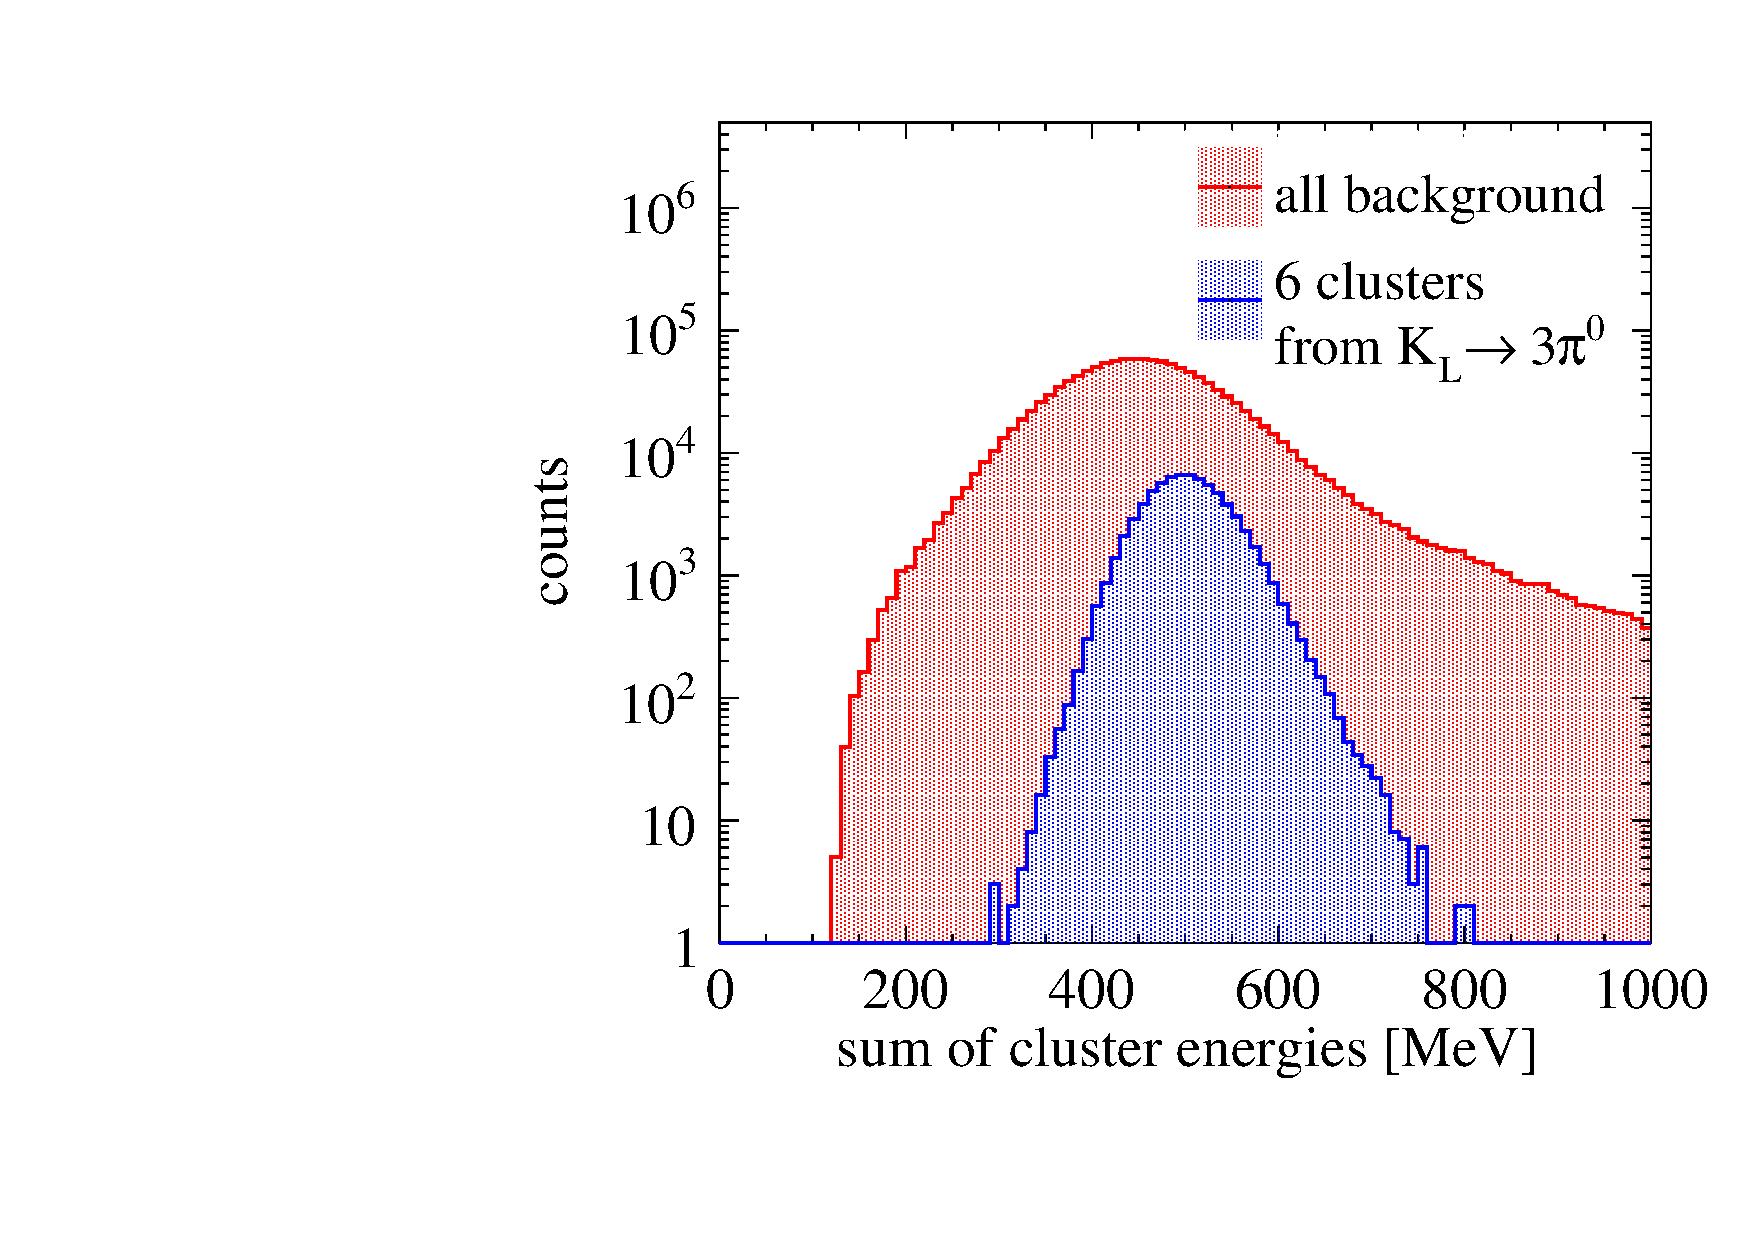
\includegraphics[width=1.0\textwidth]{Chapter7_analysis_kloe/img/e_sum}};
      \draw[black, thick, dashed] (2.95,0.8) -- (2.95,5.46);
      \draw[black, thick, dashed] (4.81,0.8) -- (4.81,4.0);
    \draw[ultra thick, black!70!white, <->] (2.95, 1.5) -- (4.81, 1.5);
    \end{tikzpicture}
    \caption{Total energy of 6 clusters for a correct 6-element cluster set in signal events (blue) and for background (red, contains both physical and combinatorial background).}\label{fig:kl3pi0selection:a}
  \end{subfigure}
  % SUB 2
    \begin{subfigure}{0.45\textwidth}
    \begin{tikzpicture}
      \node[anchor=south west,inner sep=0] at (0,0) 
      {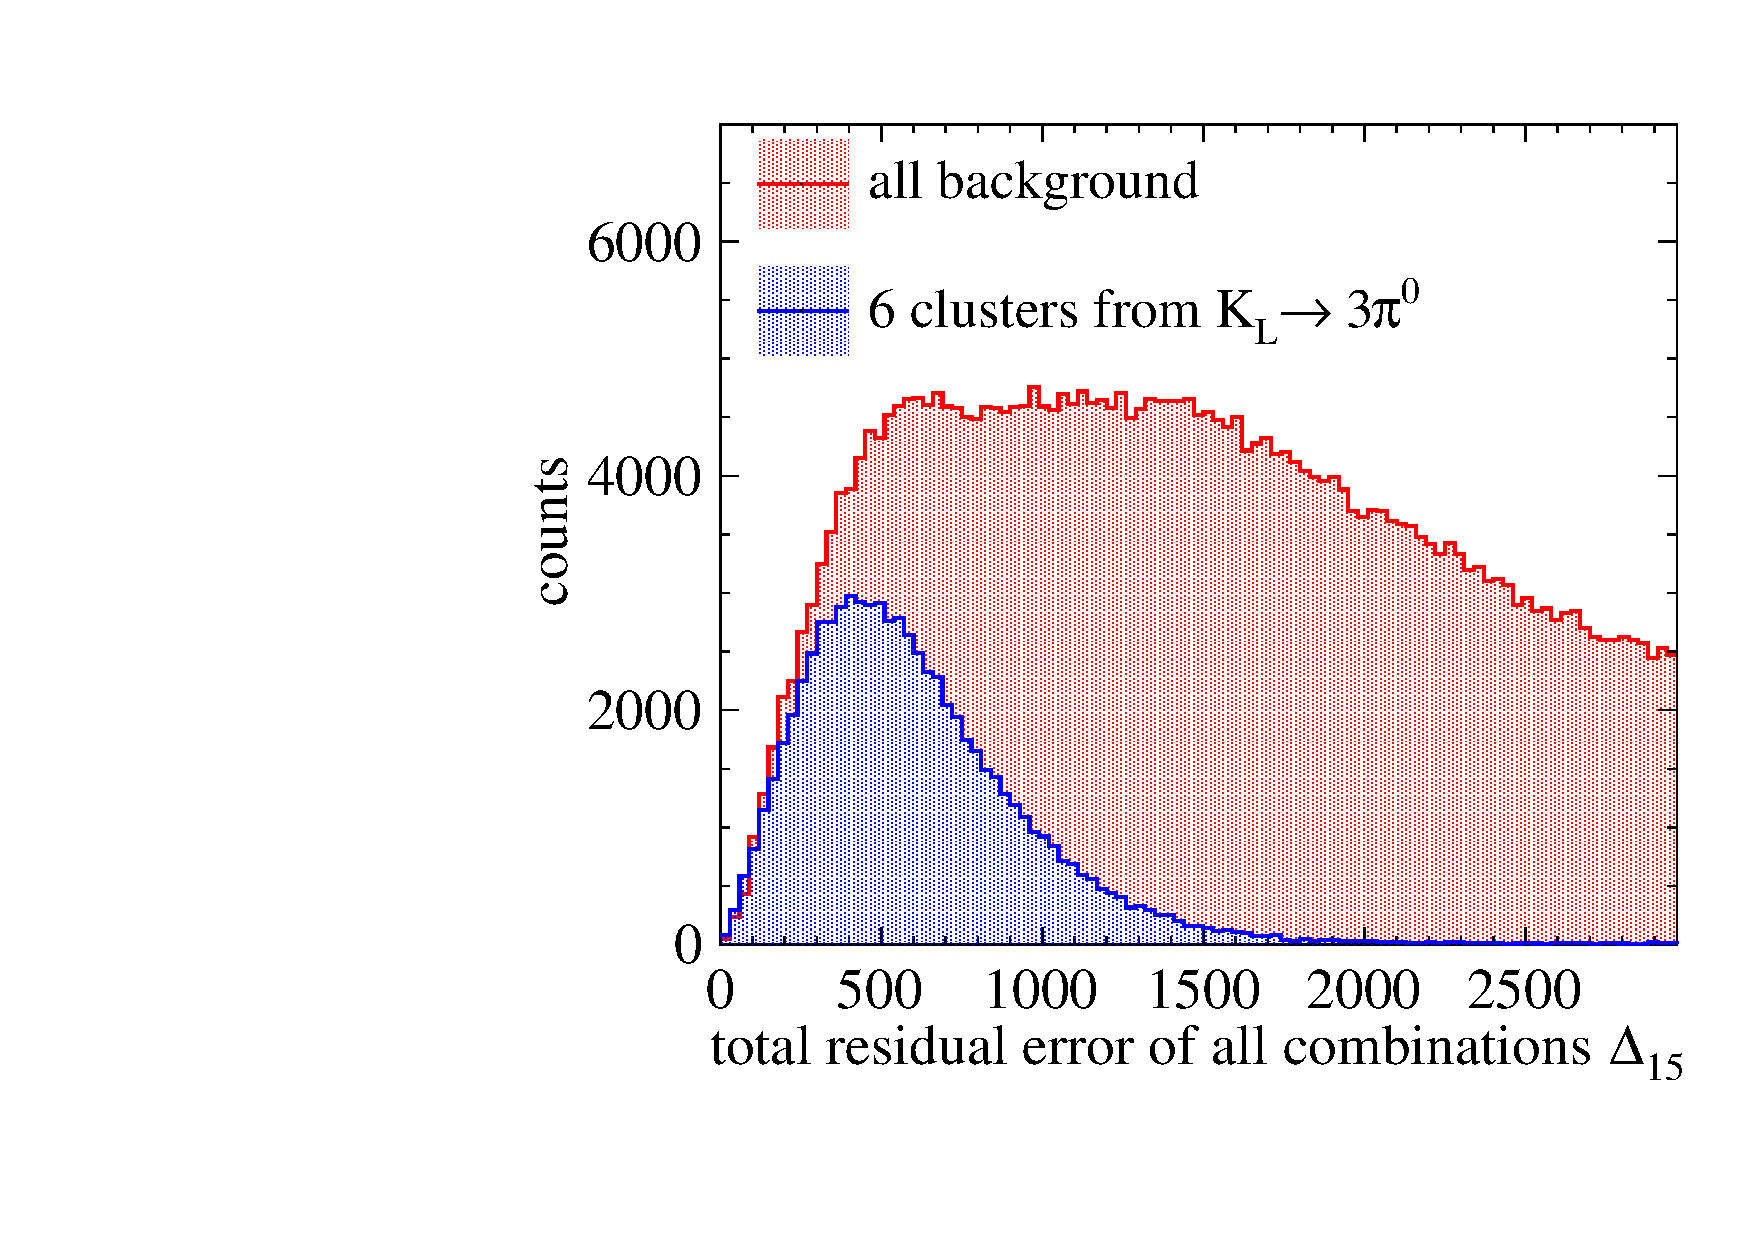
\includegraphics[width=1.0\textwidth]{Chapter7_analysis_kloe/img/residual_err}};
      \draw[black, thick, dashed] (4.8,0.8) -- (4.8,4.2);
    \draw[ultra thick, black!70!white, <-] (4.2, 1.5) -- (4.72, 1.5);
    \end{tikzpicture}
    \caption{Distribution of $\Delta_{15}$ (see~\eref{eq:delta_15}), a measure of consistency of a 6-cluster set with the $\Kl \to 3\pi^0\to 6\gamma$ hypothesis. Background plot (red) contains both physical and combinatorial background.}\label{fig:kl3pi0selection:b}
  \end{subfigure}
  % SUB 3
    \begin{subfigure}{0.45\textwidth}
    \begin{tikzpicture}
      \node[anchor=south west,inner sep=0] at (0,0) 
      {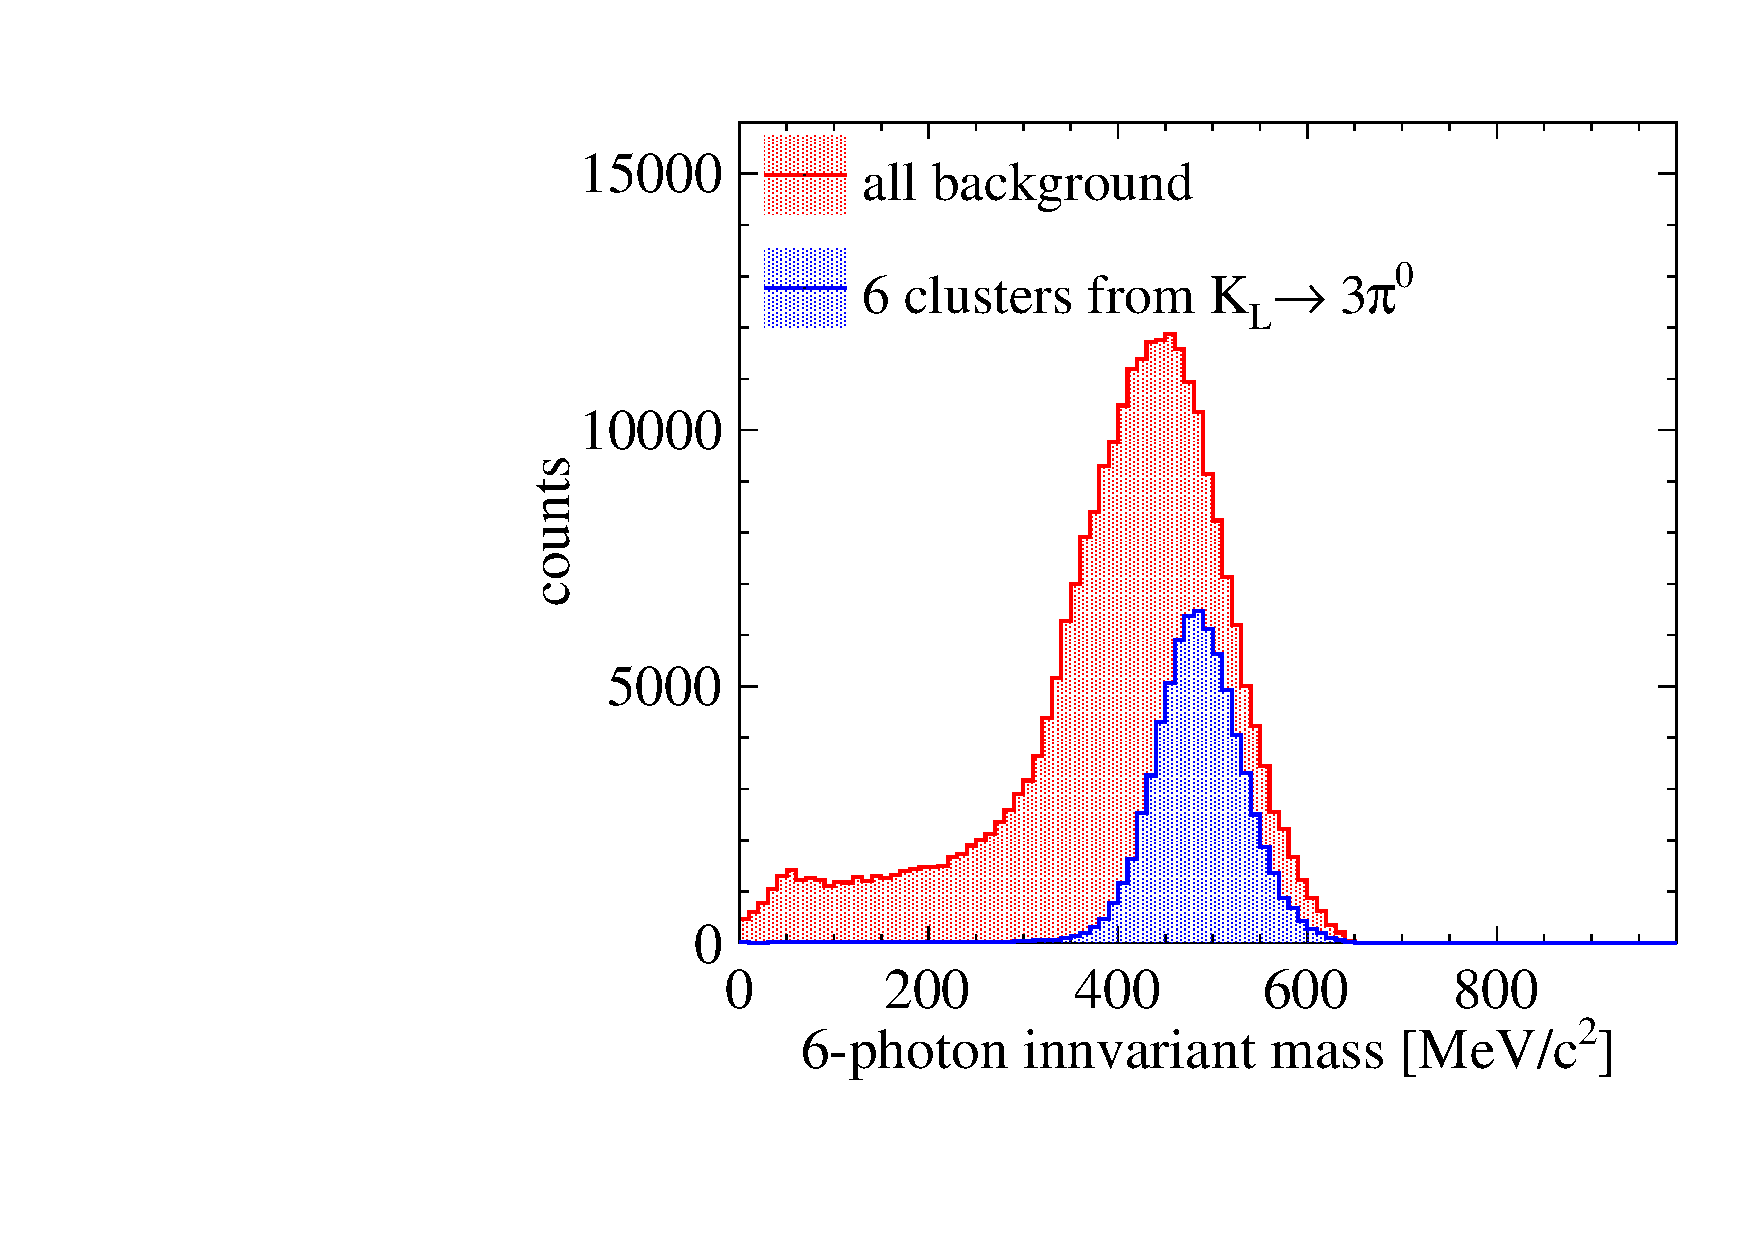
\includegraphics[width=1.0\textwidth]{Chapter7_analysis_kloe/img/6_invmass}};
      \draw[black, thick, dashed] (3.1,0.8) -- (3.1,4.2);
      \draw[ultra thick, black!70!white, ->] (3.14, 2.2) -- (3.5, 2.2);
    \end{tikzpicture}
    \caption{Invariant mass of original $\Kl$ reconstructed using 6 hypothetical photons associated to the clusters. Background plot (red) contains both physical and combinatorial background.}\label{fig:kl3pi0selection:c}
  \end{subfigure}
  % SUB 4
    \begin{subfigure}{0.45\textwidth}
    \begin{tikzpicture}
      \node[anchor=south west,inner sep=0] at (0,0) 
      {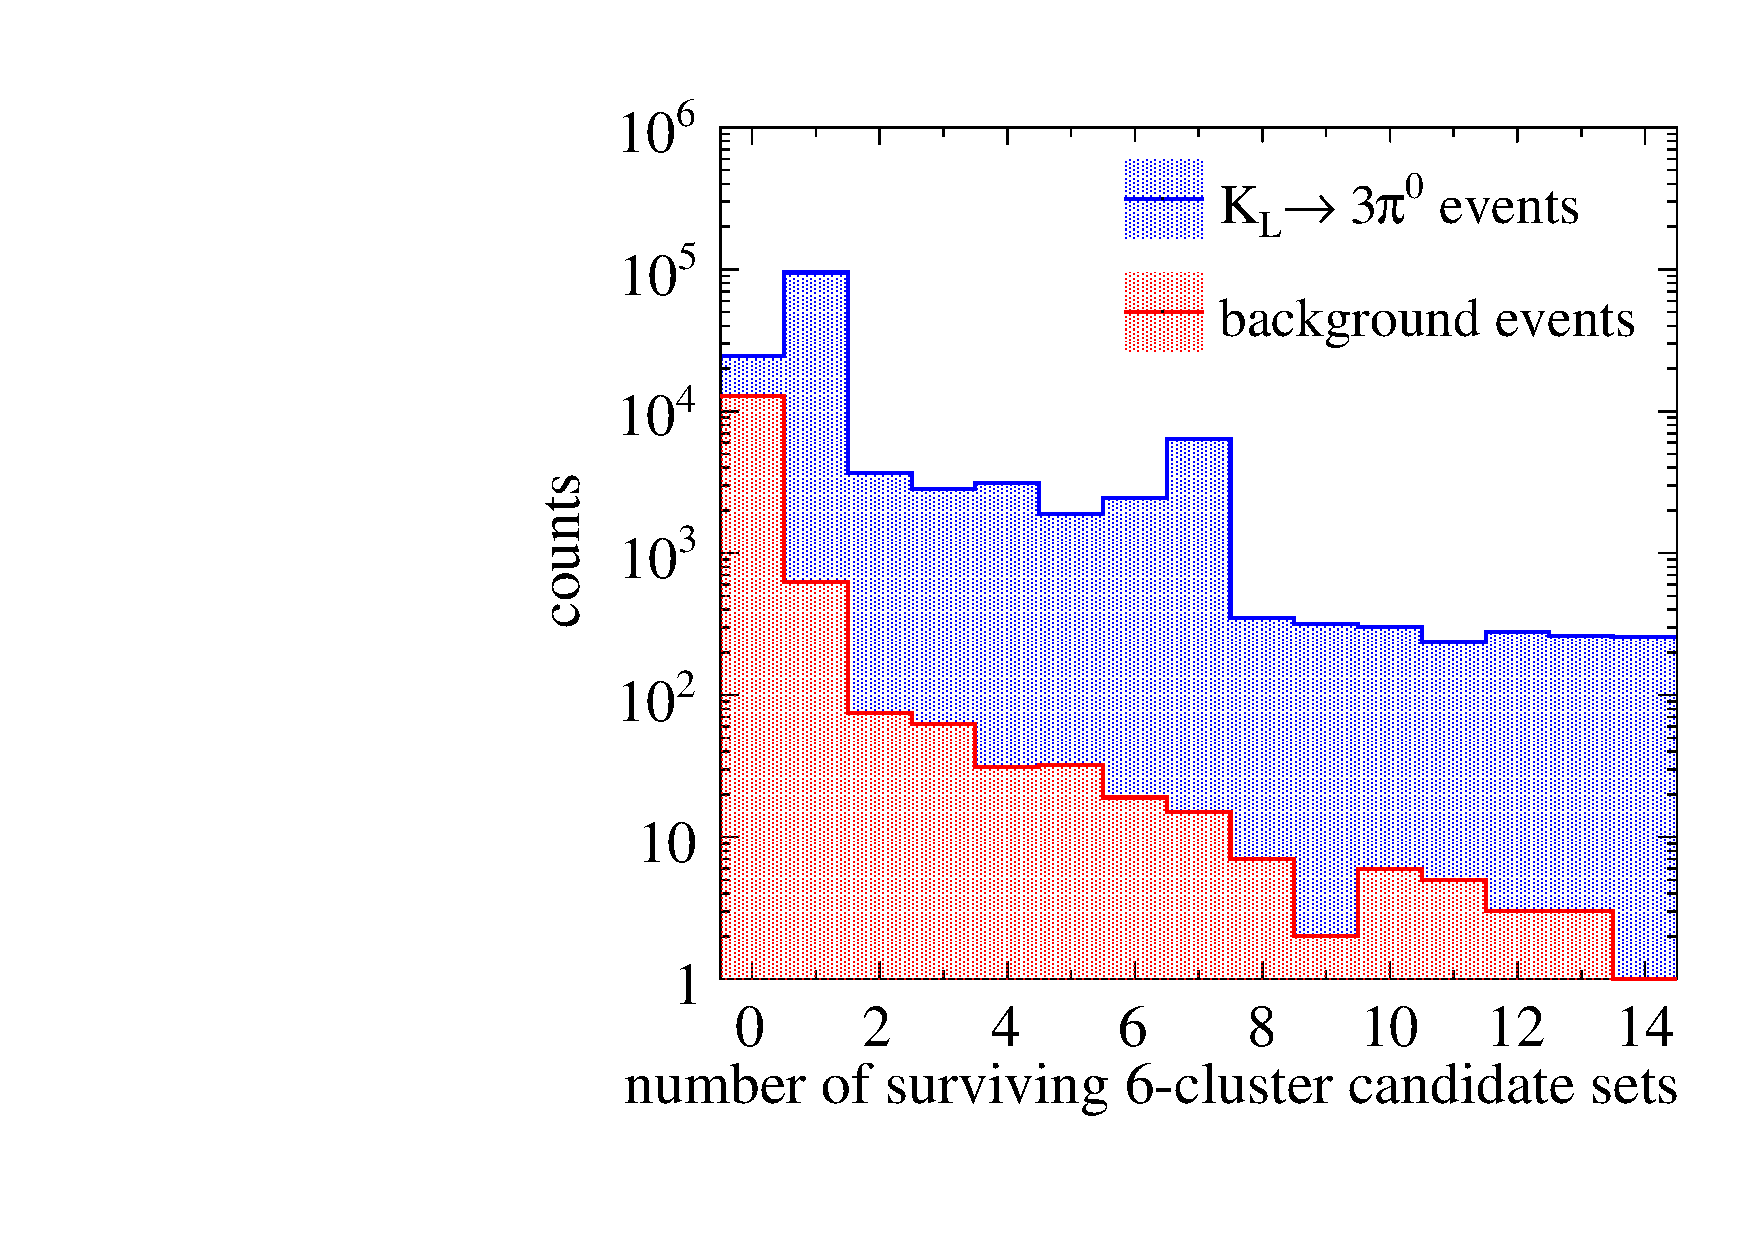
\includegraphics[width=1.0\textwidth]{Chapter7_analysis_kloe/img/surviving_sets}};
      \draw[ultra thick, black!70!white, ->] (1.49, 5.4) -- (1.84, 5.4);
      \draw[black, thick, dashed] (1.45,0.8) -- (1.45,5.46);
    \end{tikzpicture}
    \caption{Number of 6-cluster candidate sets passing the criteria depicted with dashed lines in panels A--C. Events with at least 1 surviving set are retained for further analysis.}\label{fig:kl3pi0selection:d}
  \end{subfigure}
  \caption{MC-based distributions of the variables used for selection of 6-cluster sets among all combinatorial possibilities in an event. Dashed vertical lines denote the cuts used and gray arrows indicate the accepted distribution regins.}
  \label{fig:kl3pi0selection}
\end{figure}

The second criterion applied to 6-cluster sets is based on the consistency of decay properties reconstructed using particular 4-cluster subsets. In the trilateration-based method described in~\sref{sec:gps_kloe} finding an analytical solution only requires 4 reference points, therefore all possible ${6\choose 4}=15$ choices of 4-cluster subsets are subsequently used to reconstruct the $\Kl\to 3\pi^0$ decay point and time. Each time, the obtained solution is inserted into the two equations left out (labeled $j$ and $k$) and their residual error is calculated as~(compare~\eref{eq:gps_6_eqns}):
\begin{equation}
  \label{eq:residual_error}
  \begin{split}
  r_{jk} & =  \left((X_j-x_{jk})^2 + (Y_j-y_{jk})^2 + (Z_j-z_{jk})^2 - c^2(T_j-t_{jk})^2\right)\\
  & + \left( (X_k-x_{jk})^2 + (Y_k-y_{jk})^2 + (Z_k-z_{jk})^2 - c^2(T_k-t_{jk})^2   \right).
  \end{split}
\end{equation}
where $(x_{jk},y_{jk},z_{jk},t_{jk})$ is the reconstruction result obtained by leaving out equations $j$ and $k$. For a set of 6 clusters all created by $\gamma$ quanta from the same decay, the residuals of the remaining equations should be small independently of the choice of 4 clusters used to find the decay point and time. However, if one or more clusters is not related to the decay, certain combinations will yield solutions inconsistent with the unused reference points. Therefore, the sum of residual errors for unused equations computed for all 15 possible 4-cluster set choices:
\begin{equation}
  \Delta_{15} = \sum_{j=1}^{6}\sum_{k=j+1}^{6} r_{jk},
  \label{eq:delta_15}
\end{equation}
constitutes a measure of a 6-cluster set consistency with a $\Kl \to 3\pi^0\to 6\gamma$ hypothesis useful for discrimination of wrong combinations as well as non-$3\pi^0$ background as shown in~\fref{fig:kl3pi0selection:b}. Combinations with $\Delta_{15}>2000$ are rejected.

Finally, reconstruction of invariant mass of the original neutral K meson is attempted using momenta of the supposed photons associated with the 6 clusters in the set under consideration. The $\gamma$ momenta are estimated using directions from the reconstructed $\Kl\to 3\pi^0$ decay point to the clusters' locations and the clusters' energies. \fref{fig:kl3pi0selection:c} presents the resulting 6-photon invariant mass distributions, where 6-cluster combinations are rejected if $M_{6\gamma} < 350\:\text{MeV/c}^2$.

The number of 6-cluster combinations which satisfy all of the above criteria is shown in~\fref{fig:kl3pi0selection:d}. Events where no candidate cluster sets survive are rejected. The ``plateau'' region extending between 1 and 7 sets arises from the relatively high probability of total 7 candidate clusters in an event (compare~\fref{fig:t1-early-cuts}, Right) as several consistent 6-cluster sets can be found e.g.\ due to splitting of a cluster originating from a signal event. In order to maximize selection efficiency, events with more than 1 candidate cluster set are retained for the analysis. In such cases, the set is chosen which minimizes the $\Delta_{15}$ consistency measure.

% TODO: dopisac, dlaczego rozdzielczosc w funkcji odleglosci of phi
Once an event is identified as $\Kl\to 3\pi^0$ by the presence of at least one candidate set of 6 clusters, reconstruction of the decay point and time using the trilateration technique can be attempted in several manners:
\begin{itemize}
\item using a mean solution obtained from all ${6\choose 4}$ possible choices of a subset of 4 out of 6 clusters (referred to as \textit{mean analytical} in~\fref{fig:resolutions_nofit}),
\item using the subset of 4 equations for which the residual error (see~\eref{eq:residual_error}) was smallest (\textit{best analytical} in~\fref{fig:resolutions_nofit}); this has the advantage of being able to yield a correct solution even if the chosen 6-cluster set is contaminated,
\item solving the system for all 6 reference points with iterative least squares method to minimize measurement uncertainties.
\end{itemize}

\begin{figure}[h!]
  \centering
  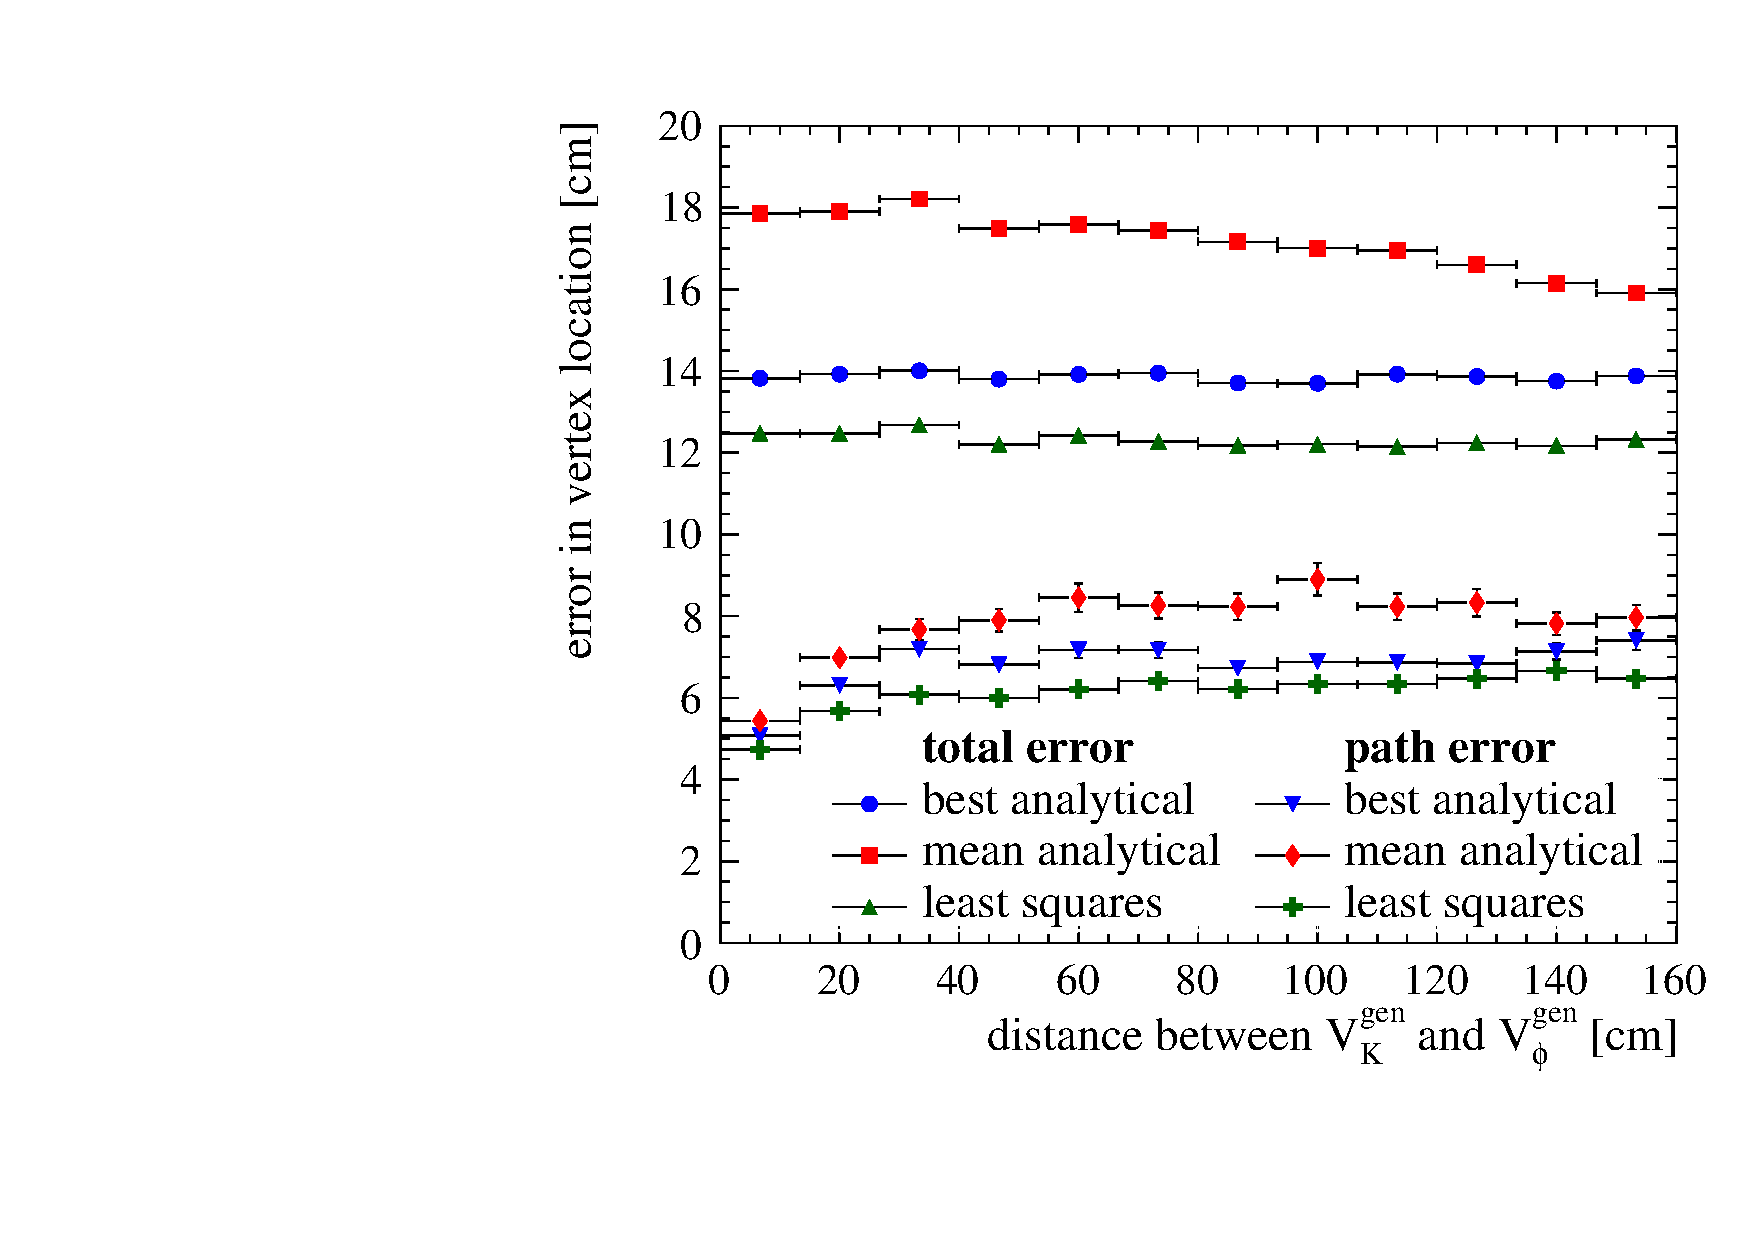
\includegraphics[width=0.5\textwidth]{Chapter7_analysis_kloe/img/resolutions_nofit}
  \caption{MC-based study of the resolution of $\Kl\to 3\pi^0$ decay vertex reconstruction expressed as total error on reconstructed w.r.t.\ MC-generated location of the decay point, as well as error on determination of the kaon travelled path, for subsequent ranges of decay distance from $\phi$. Three different reconstruction methods are presented.}\label{fig:resolutions_nofit}
\end{figure}

The resolution available with each of these approaches was studied using a sample of MC-simulated $\Kl\to 3 \pi^0$ events for which the choice of 6 clusters used for decay reconstruction was done as described above. As the performance of reconstruction may change with decay vertex location in the detector, resolution was studied as the distance between MC-generated and reconstructed decay point for multiple regions of decay distance from the $\phi$ decay. In addition to the total error in determination of the decay vertex position, the error on path travelled by the kaon was studied as being relevant to the calculation of decay time, needed for the \Ts~symmetry test. \fref{fig:resolutions_nofit} shows results of the resolution studies, from which it is evident that the numerical (least squares) solution using all 6 clusters as reference points allows for the most accurate determination of the $\Kl$ decay point. However, the error on the kaon travelled path at the 6~cm level still corresponds to about 1~ns uncertainty in the $\Kl$ decay time whereas the desired temporal resolution for the \Ts~test should be $\order{1\:\tau_S}\approx\order{0.1\:\text{ns}}$. Therefore, at a later analysis stage the decay time resolution is further enhanced with a dedicated kinematic fit described in~\sref{sec:kinfit}.
%
% TODO: wydajności oraz % identyfikacji dobrego zestawu klastrów
%

\subsection{Estimation of $\Ks$ momentum}\label{sec:ks_from_kl}
The selection of semileptonic decays of $\Ks$ presented in the next Sections relies partially on an estimate of the momentum vector of this kaon. However, momentum of the escaping neutrino prevents a precise reconstruction of $\vec{p_{K_S}}$ using a sum of the recorded products' momenta. Alternatively, the $\Ks$ momentum can be inferred from momentum conservation for the $\phi\to\Ks\Kl$ decay using the associated long-lived neutral kaon. $\phi\to\Ks\Kl$, as a two-body decay into particles of identical mass, produces both kaons with equal energies and opposite momenta in the center-of-mass frame of reference:
\begin{equation}
  \label{eq:momentum_tagging}
  p_{K}^{CM} = \sqrt{\frac{1}{4}m_{\phi}^2-m_{K_0}^2}.
\end{equation}
which moves with respect to the laboratory system with the momentum of initial $\phi$~meson, defined by properties of colliding electron and positron beams (see~\sref{sec:dafne}). The Lorentz transformation required to know the momenta of $\Ks$ and $\Kl$ in the laboratory frame only acts on the their components parallel to $\vec{p_{\phi}}$. Therefore, the complete kinematical configuration of a $\phi\to\Ks\Kl$ event, including moduli and momenta of both neutral kaons, depends only on the angle of their emission with respect to the $\phi$ momentum. Consequently, to determine $\vec{p}_{K_S}$ and $\vec{p}_{K_L}$, it is sufficient to know the direction of momentum of one of the kaons~\cite{daria_memo}. This can be estimated in a number of ways in the $\Ks \Kl \to \pi^{\pm}e^{\mp}\nu\:3\pi^0$ events:
\begin{enumerate}
\item using the vector spanning between the $\phi$ decay point and $\Ks\to\pi e\nu$ vertex obtained from DC tracks as direction of the $\Ks$ momentum,
\item using the vector spanning between the $\phi$ decay point and $\Kl\to 3\pi^{0}$ decay point obtained with the trilaterative reconstruction as direction of the $\Kl$ momentum,
\item using the $\Kl$ momentum obtained from a sum of the 6 photons' momenta calculated from their corresponding $\Kl$ vertex--EMC cluster directions and energies deposited in the clusters.
\end{enumerate}

\begin{figure}[h!]
  \centering
  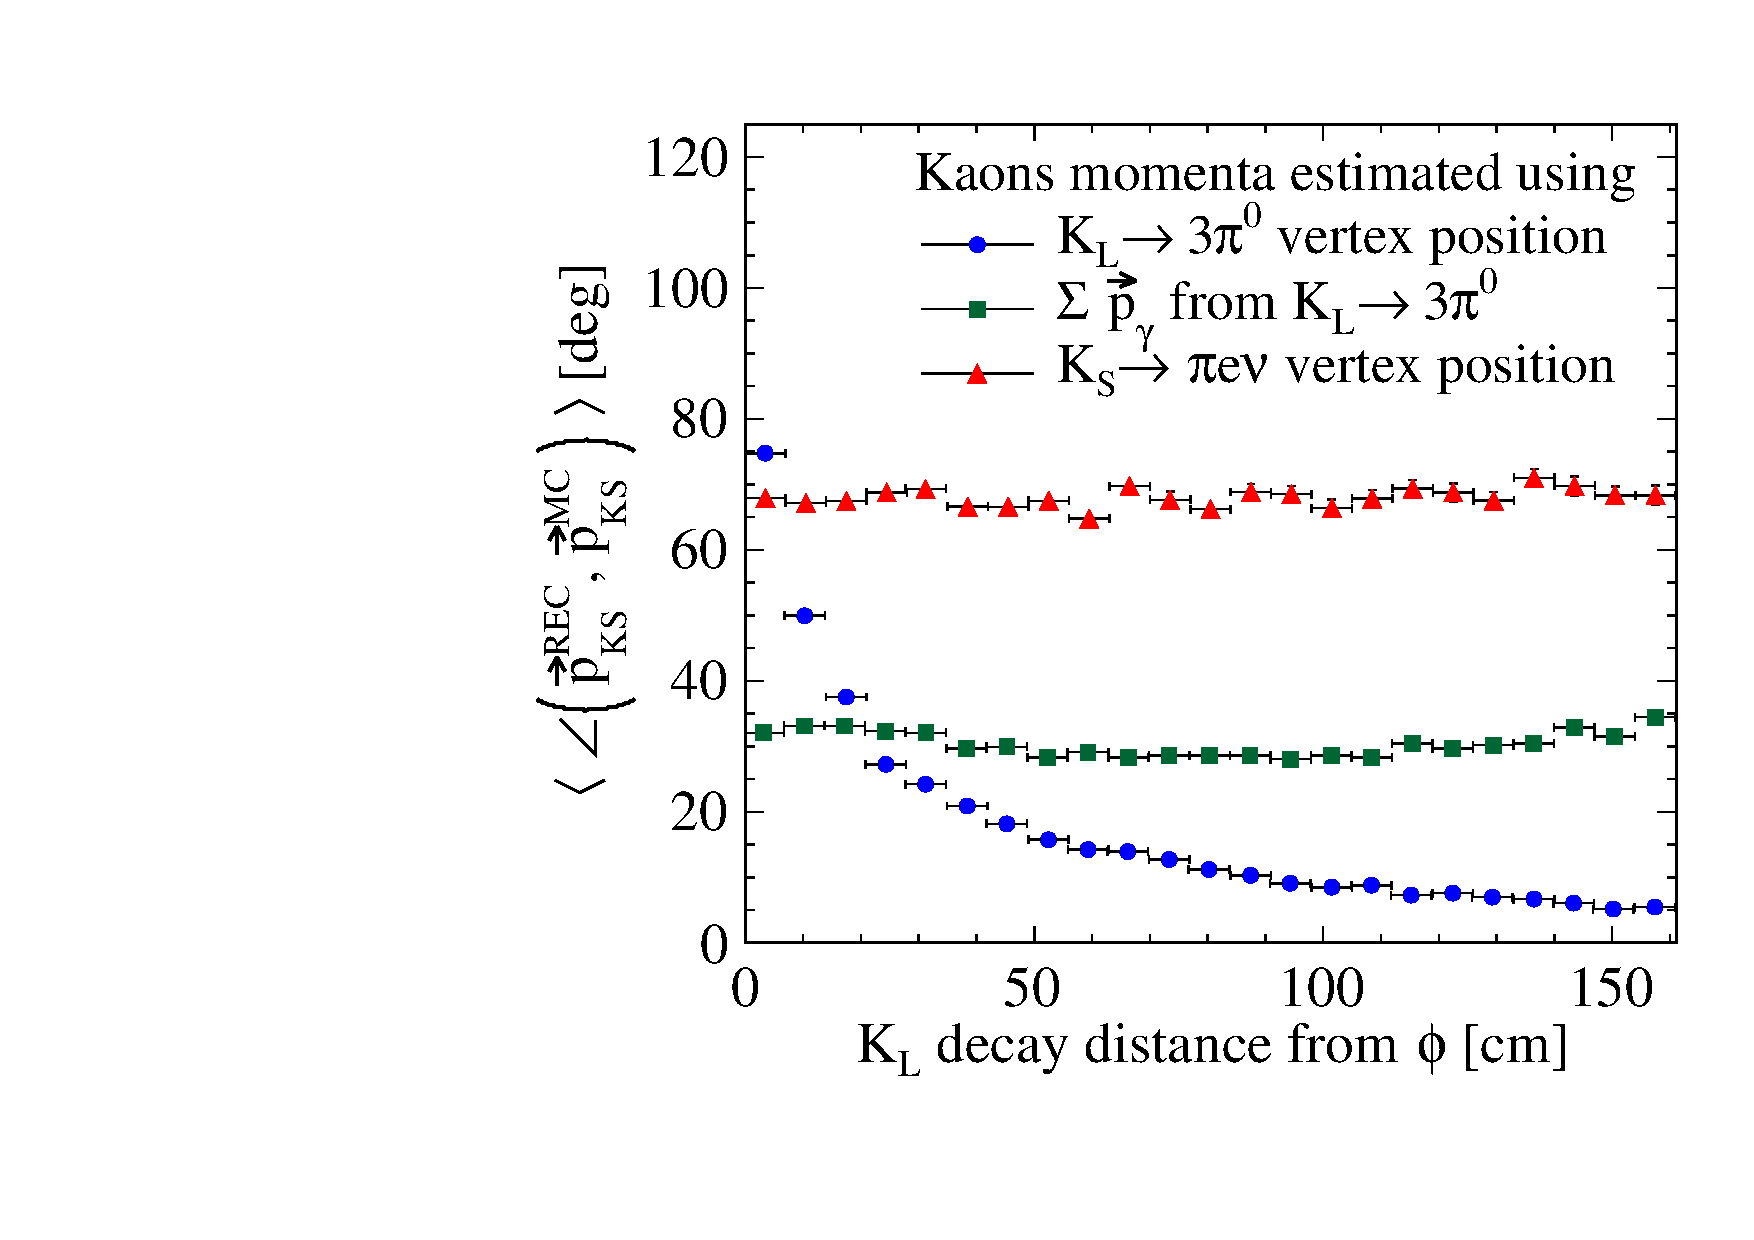
\includegraphics[width=0.45\textwidth]{Chapter7_analysis_kloe/img/ks_angle_resolution}
  \hspace{1em}
  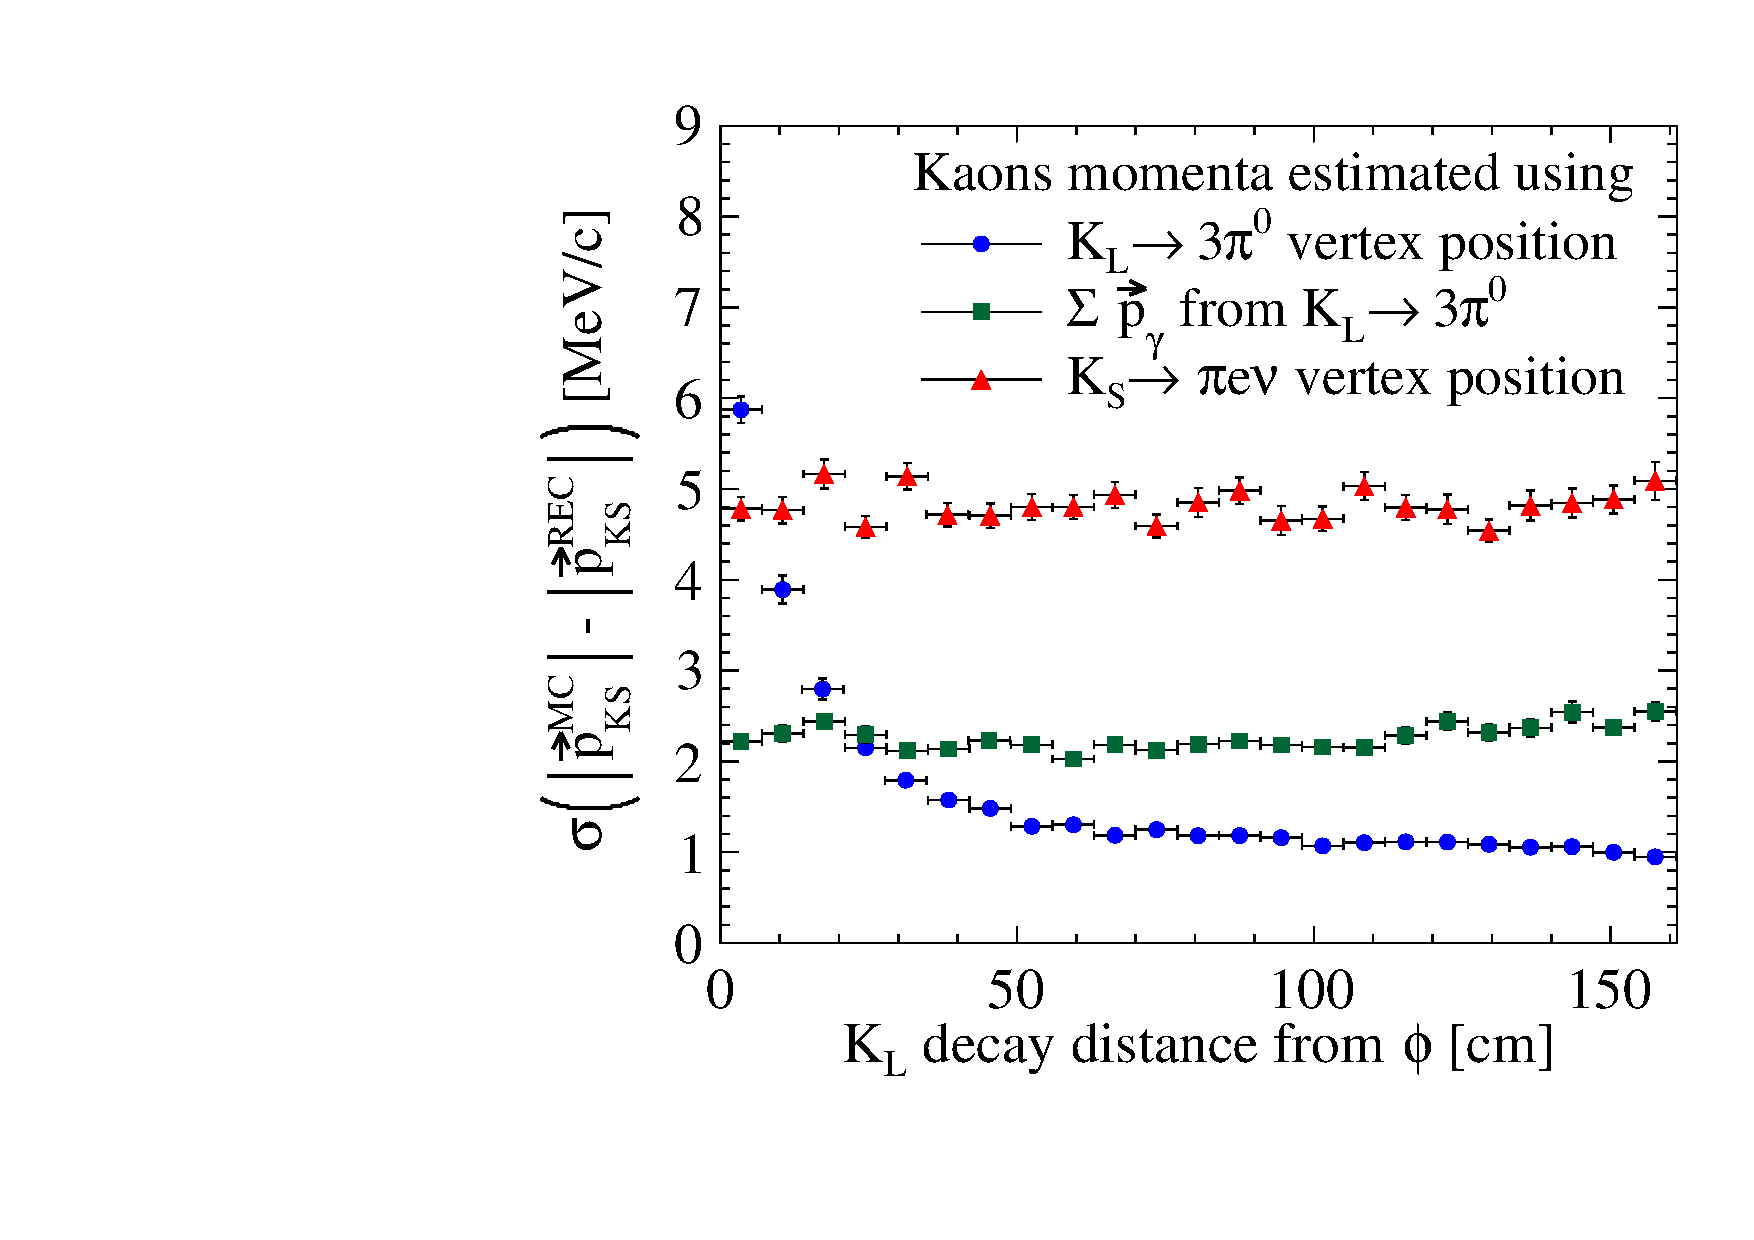
\includegraphics[width=0.45\textwidth]{Chapter7_analysis_kloe/img/ks_modulus_resolution}
  \caption{Resolution of direction (left) and modulus (right) of the $\Ks$ momentum estimated using the kinematics of 2-body $\phi\to\Ks\Kl$ decay and three kinds of available information on kaons' momentum directions.}\label{fig:ks_angle_resolution}
\end{figure}

\fref{fig:ks_angle_resolution} presents a comparison of the resolutions of $\Ks$ momentum in terms of its direction (left) and modulus (right), along with their dependence on the distance of $\Kl$ decay from the primary interaction point, obtained with momentum conservation for the $\phi\to \Ks\Kl$ decay and the three approaches to evaluate a kaon momentum direction listed above. Method 1 (red in~\fref{fig:ks_angle_resolution}) does not exhibit any resolution variations with the $\Kl$ decay position being based solely on information related to $\Ks$. Although it uses the precise position of $\Ks\to\pi e\nu$ vertex obtained with the drift chamber, larger uncertainty on the average $\phi$ decay point and the fact that both points are located close to each other result in large errors on the $\Ks$ momentum. While the same uncertainty of average $\phi$ vertex influences the second approach (blue), significantly larger possible distances between the two considered points provide better resolution of $\vec{p}_{K_S}$ which improves with distance between $\Kl$ decay and $\phi$. For early $\Kl$ decays, however, performance of this technique is reduced due to a relatively low resolution of the $\Kl\to 3\pi^{0}$ vertex location. The third estimation method (green) does not directly utilize information on decay vertices, instead relying on photons' momentum information reconstructed using the $\Kl$ decay point and EMC cluster energies. Resolution of this method, constant independently of the $\Kl$ decay distance, is superior to the other approaches for the events with early decays of $\Kl$.

In order to obtain the best estimate of $\vec{p}_{K_S}$ for the use in next analysis steps, the following strategy was adopted:
\begin{itemize}
\item using $\Kl\to 3\pi^{0}$ vertex position (method 2) if $|V_{\Kl}-V_{\phi}| > 20$~cm,
\item using $\sum \vec{p}_{\gamma}$ (method 3) if $|V_{\Kl}-V_{\phi}| \leq 20$~cm.
\end{itemize}

\subsection{Selection of semileptonic $\Ks$ decays}\label{sec:ksemil}
The most abundant background for the semileptonic $\Ks$ decays is constituted by the two-pion final states $\pi^+\pi^-$ and $\pi^0\pi^0$ which together account for~\SI{99.89}{\percent} of all decays of this meson. While the $\pi^0\pi^0$ is easily differentiated by the lack of charged particle tracks recorded in the KLOE drift chamber%
\footnote{In fact, $\Ks\to\pi^0\pi^0$ may be confused with an early $\Kl\to 3\pi^0$ decay when the accompanying kaon produces a semileptonic final state. Identification of such cases is discussed in~\sref{sec:ks2pi0_rejection}.},
$\pi^+\pi^-$ must be distinguished from the signal $\pi e\nu$ events using kinematical properties of the two recorded tracks.

In the center of mass reference frame, the $\Ks\to\pi^+\pi^-$ process is characterized by momenta of both products being exactly opposite whereas the angle between momenta of the two recorded particles in a semileptonic decay come from a broad spectrum with small probability of a back-to-back decay. The first step of selection of $\Ks\to\pi e\nu$ is therefore based on the angle $\alpha_{CM}$ constituted by momenta associated to the two recorded DC tracks at their common vertex, expressed in the center-of-mass frame. To this end, momenta reconstructed in the detector frame were subjected to a Lorentz transformation to the $\Ks$ frame of reference using its momentum estimated as shown in the previous Section. The obtained distributions of the $\alpha_{CM}$ angle are presented in the left panel of~\fref{fig:ksemil_basic_cuts} where signal is defined as events with the $\Ks\to\pi e\nu$ decay and background is dominated by $\Ks\to\pi^+\pi^-$. Events were retained for further analysis if:
\begin{equation*}
   \ang{40} < \alpha_{CM} < \ang{170}.
\end{equation*}

\begin{figure}[h!]
  \centering
  \begin{tikzpicture}
    \node[anchor=south west,inner sep=0] at (0,0) 
    {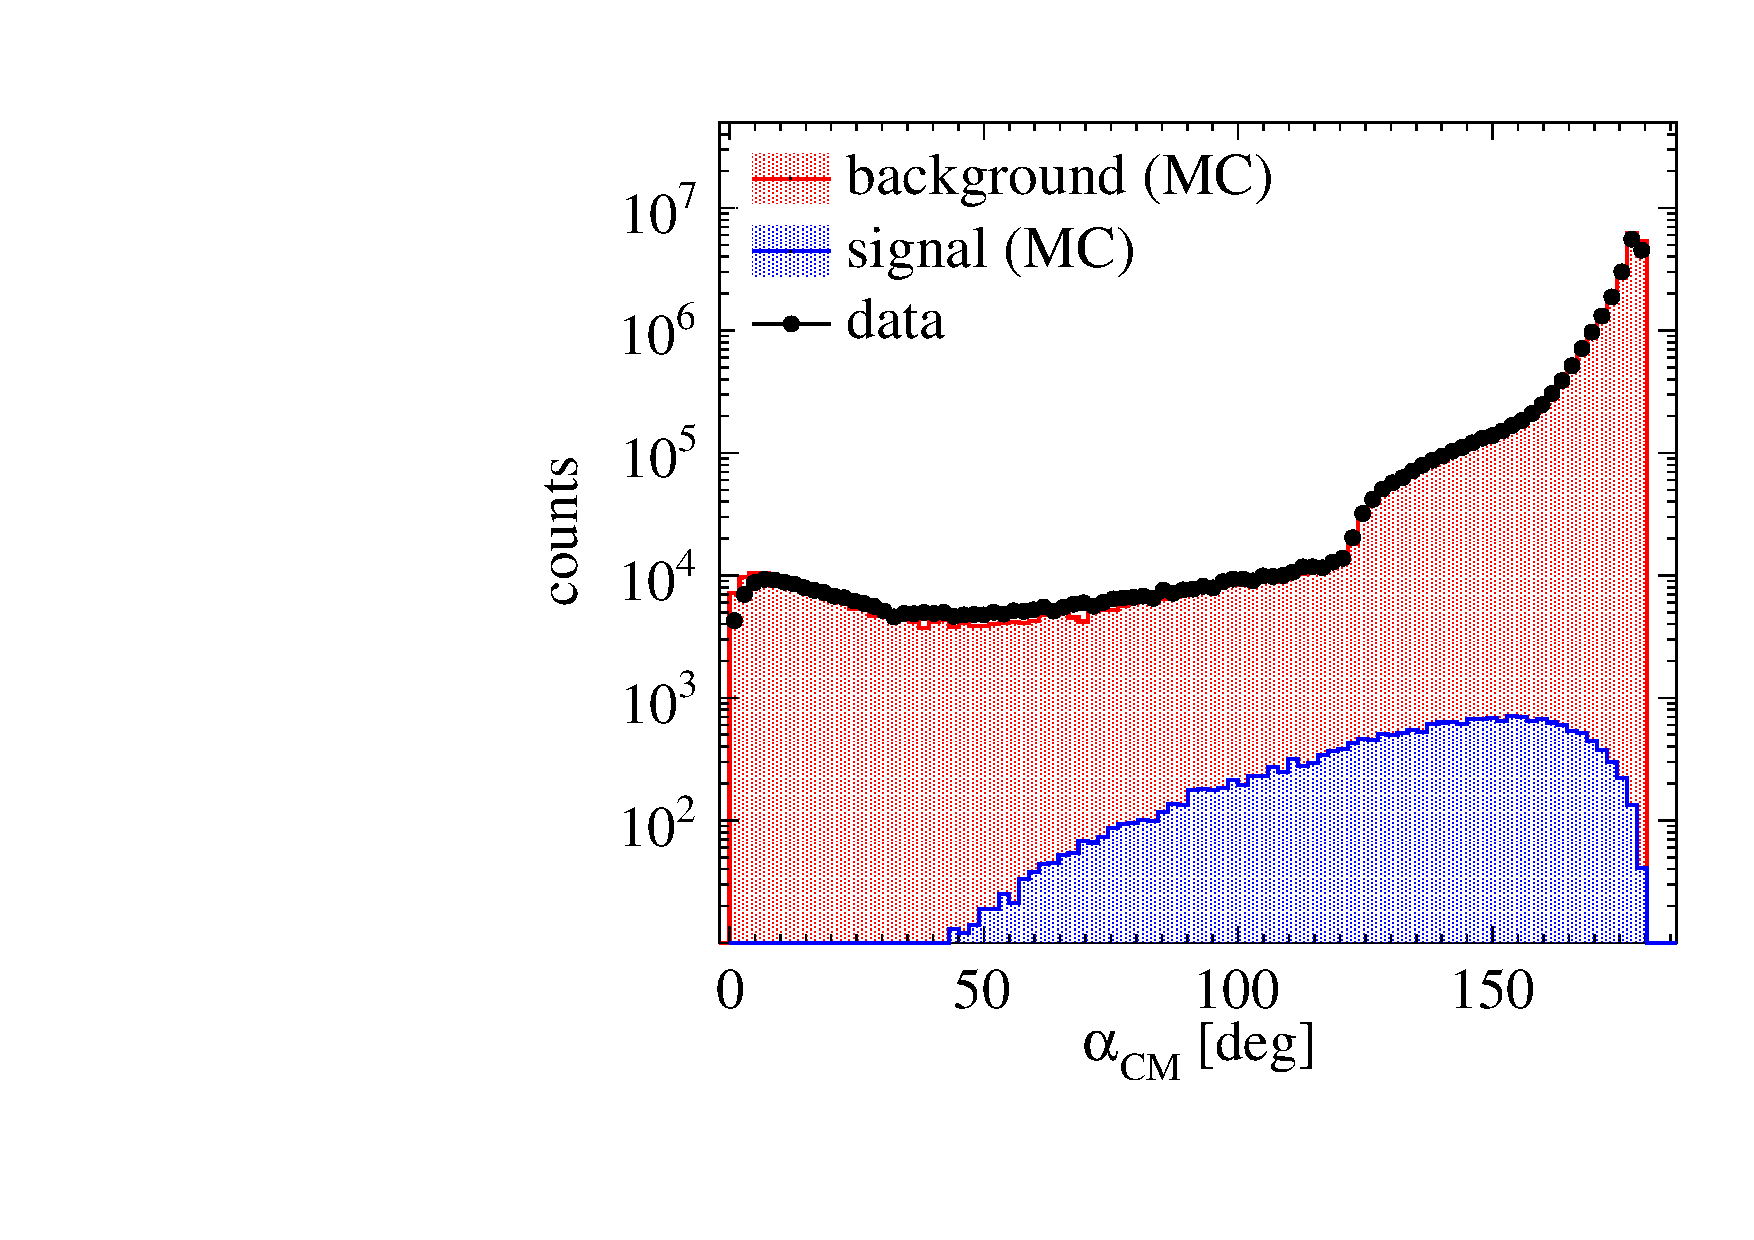
\includegraphics[width=0.45\textwidth]{Chapter7_analysis_kloe/img/alpha_cm}};
    \draw[black, thick, dashed] (2.32,0.8) -- (2.32,4.1);
    \draw[black, thick, dashed] (6.1,0.8) -- (6.1,5.46);
  \end{tikzpicture}
  \hspace{1em}
    \begin{tikzpicture}
    \node[anchor=south west,inner sep=0] at (0,0) 
    {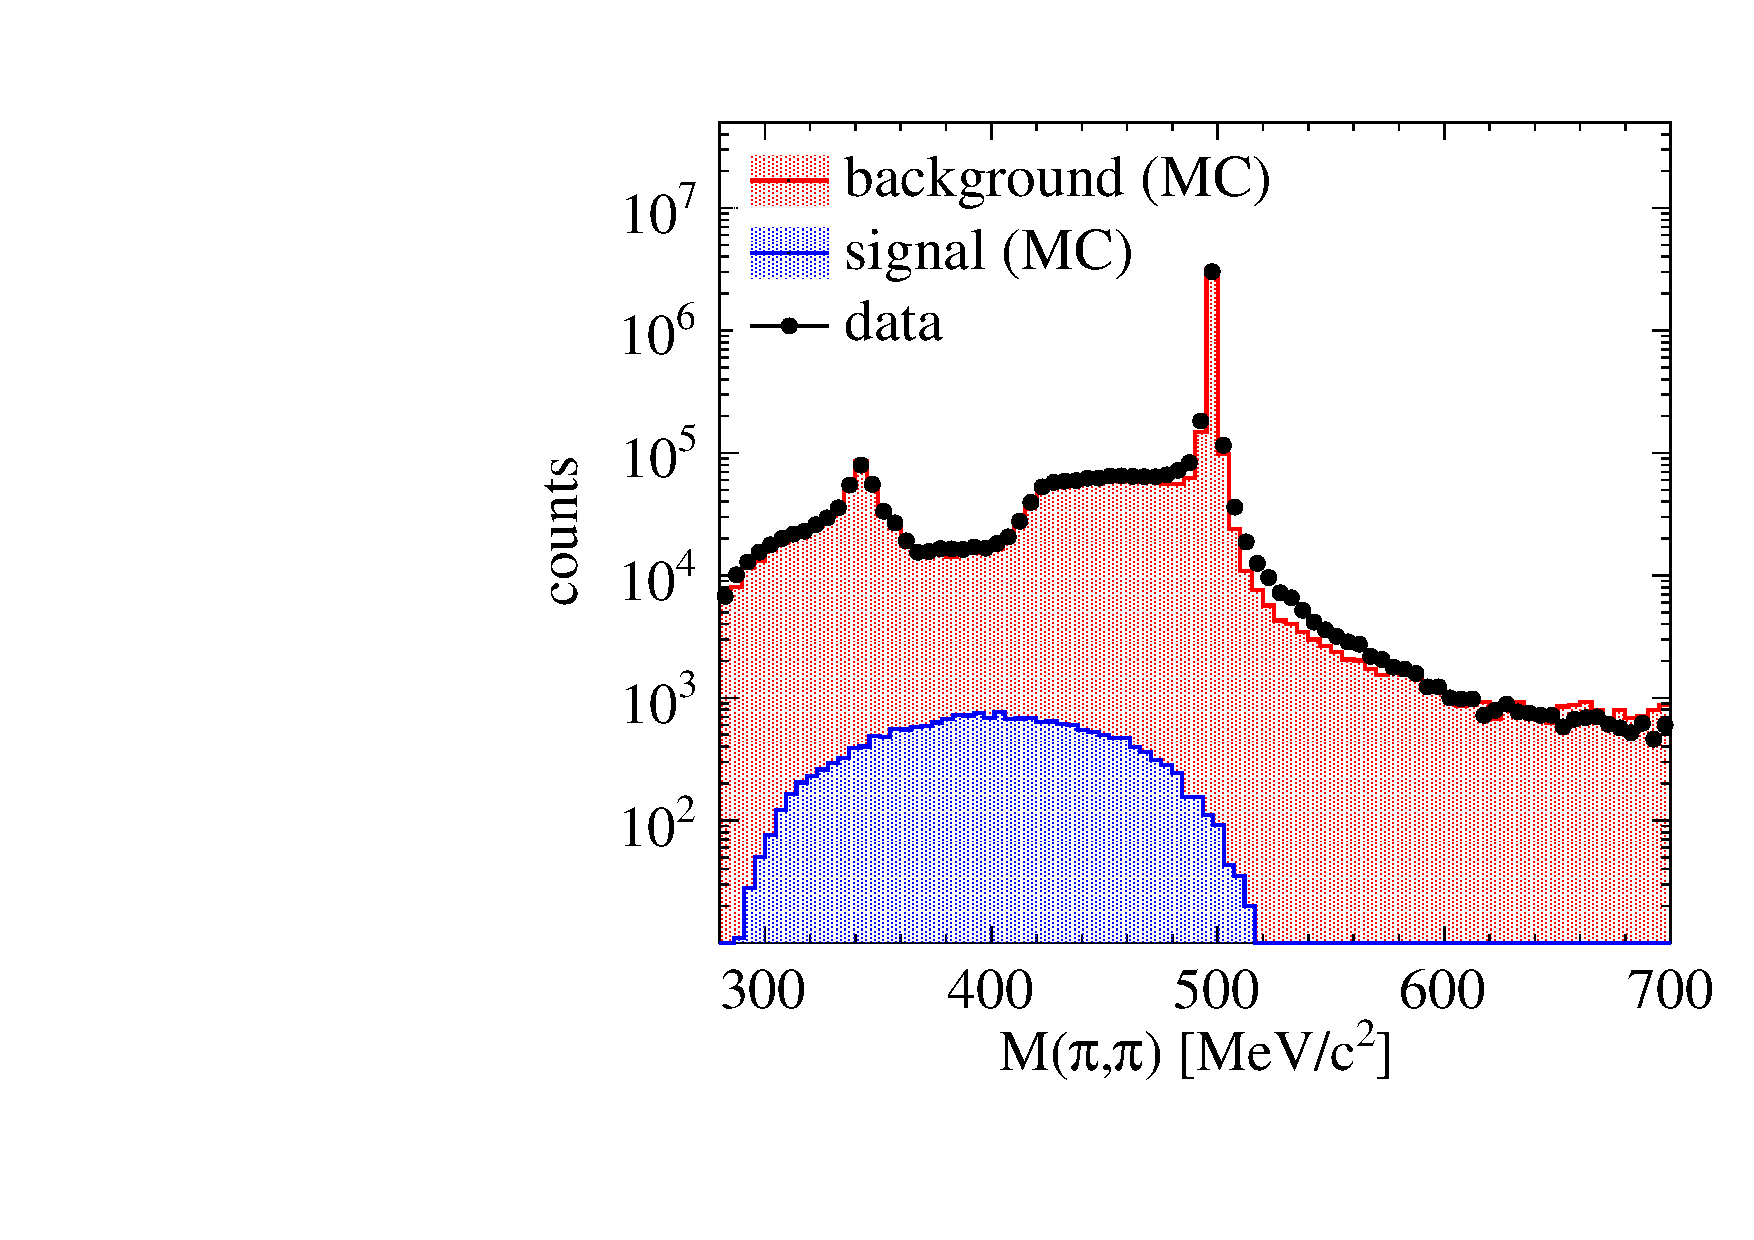
\includegraphics[width=0.45\textwidth]{Chapter7_analysis_kloe/img/invmass}};
    \draw[black, thick, dashed] (3.81,0.8) -- (3.81,5.0);
  \end{tikzpicture}
  \caption{Distributions used for preselection of semileptonic $\Ks$ decays (referred to as \textit{signal}). Dashed lines denote the values of cuts. Left: Angle between momenta of the two decay products whose tracks are recorded by the KLOE DC, expressed in the center-of-mass reference frame. Right: invariant mass of the decaying state calculated with momenta of the two recorded decay products assuming that both were charged pions.}
  \label{fig:ksemil_basic_cuts}
\end{figure}

At the event preselection stage, the two recorded tracks with a common vertex are not yet identified as pions, electrons or muons. Due to well-defined kinematics of $\Ks\to\pi^+\pi^-$,
invariant mass of the decaying state, calculated attributing the mass of a charged pion to both tracks, peaks at the neutral kaon mass with any possible deviation caused only by detector and reconstruction resolution. By contrast, the semileptonic decay where a neutrino carries away unknown momentum, may yield an invariant mass from a broad spectrum mostly below $m_{\kaon}$ as shown in~\fref{fig:ksemil_basic_cuts} (right). In order to reject a large part of the $\pi^+\pi^-$ background, only events for which:
\begin{equation*}
  \text{M}(\pi,\pi) < 490\:\text{MeV/c}^{2},
\end{equation*}
are processed further. After the selection of $\Kl\to 3\pi^0$ and the aforementioned $\Ks\to \pi e\nu$ preselection, the signal to background (S/B) ratio is about 0.13 which calls for a refined event selection, achieved with a time of flight (TOF) analysis of the decay products.

\subsection{Time of flight analysis for charged particles}\label{sec:t1_tof}
The analysis of time of flight is performed for particles corresponding to the two DC tracks associated to the $\Ks$ decay vertex candidate chosen at preselection stage.
The general scheme of this procedure is based on the approaches used in previous studies of $\Ks\to \pi e \nu$ at KLOE~\cite{Ambrosino:2006si,daria_article}. However, these studies allowed a certain amount of background events in the final event sample and perform a MC-based background subtraction and event counting. Moreover, they were based on events with a $\Kl$ interaction in the calorimeter which provided a high resolution of $\Kl$ and $\Ks$ momenta (calculated as discussed in~\sref{sec:ks_from_kl}). Conversely, in the analysis described in this work, kaons' momenta estimation with $\Kl\to 3\pi^0$ is not as precise and the event selection is required to yield a highly pure sample of semlileptonic decays of $\Ks$. Therefore, the details of the time of flight analysis have been adjusted to perform a more stringent event selection and additional cuts have been introduced to reject particular types of remaining background.

In addition to background discrimination, the time of flight study serves two other purposes. Firstly, it allows to identify the tracks created by pions and by electrons or positrons by testing two possible hypotheses about masses of the two charged particles in an event. Secondly, TOF information is used to calculate the correct time of the $\phi$ decay, which may be different from the DAQ start time by a multiple of the collider bunch crossing periods as discussed in~\sref{sec:trigger}.

%
% MEMO TODO: opisac i zacytowac datizza i pezzetto itd.
%
In order to calculate the expected time of flight of a particle associated with a DC track, the track is extrapolated to its incidence point on the electromagnetic calorimeter of KLOE and total length $L$ of the particle track up to its interaction in the EMC is calculated. Velocity is calculated from the momentum reconstructed for a track, with a certain assumption on the particle mass $m_x$:
\begin{equation}
  \label{eq:track_beta}
  \beta(m_x) = \frac{p}{\sqrt{p^{2}+m_x^{2}c^{2}}},
\end{equation}
so that the expected particle time of flight reads $L/(c\beta(m_{x}))$. To compare this value with a recorded particle time of flight, the particle must undergo an interaction in the calorimeter whose time $t_{cl}$ is recorded. Although such requirement removes a fraction of the signal events where poor track reconstruction or a $\pi^{\pm}\to\mu^{\pm}\nu$ decay inside the drift chamber may prevent a correct extrapolation of a track to the EMC or association to an energy deposition cluster (efficiency of this step is about \SI{43}{\percent}), it provides information which is powerful in terms of background rejection and particle identification.

For each of the two recorded tracks, a discrepancy between expected and recorded time of flight of a particle with mass $m_{x}$ is calculated as:
\begin{equation}
  \label{eq:dtof_t1}
  \delta t({m_x}) = t_{cl} - \frac{L}{c\beta(m_x)},
\end{equation}
where $x=\pi^{\pm}$ or $x=e^{\pm}$ denotes the adopted particle mass hypothesis. It should be noted that, as mentioned in~\sref{sec:trigger}, at this stage the recorded time of particle interaction in the EMC (and thus also $\delta t(m_{x})$) may be determined with respect to an incorrect event start time ($t_{0}$) and therefore all variables used in the TOF analysis are defined as differences of such values attributed to both tracks in an event. Any possible time offset, which must be common for both particles, is then cancelled out. 

\begin{figure}[h!]
  \centering
    \begin{tikzpicture}
    \node[anchor=south west,inner sep=0] at (0,0) 
    {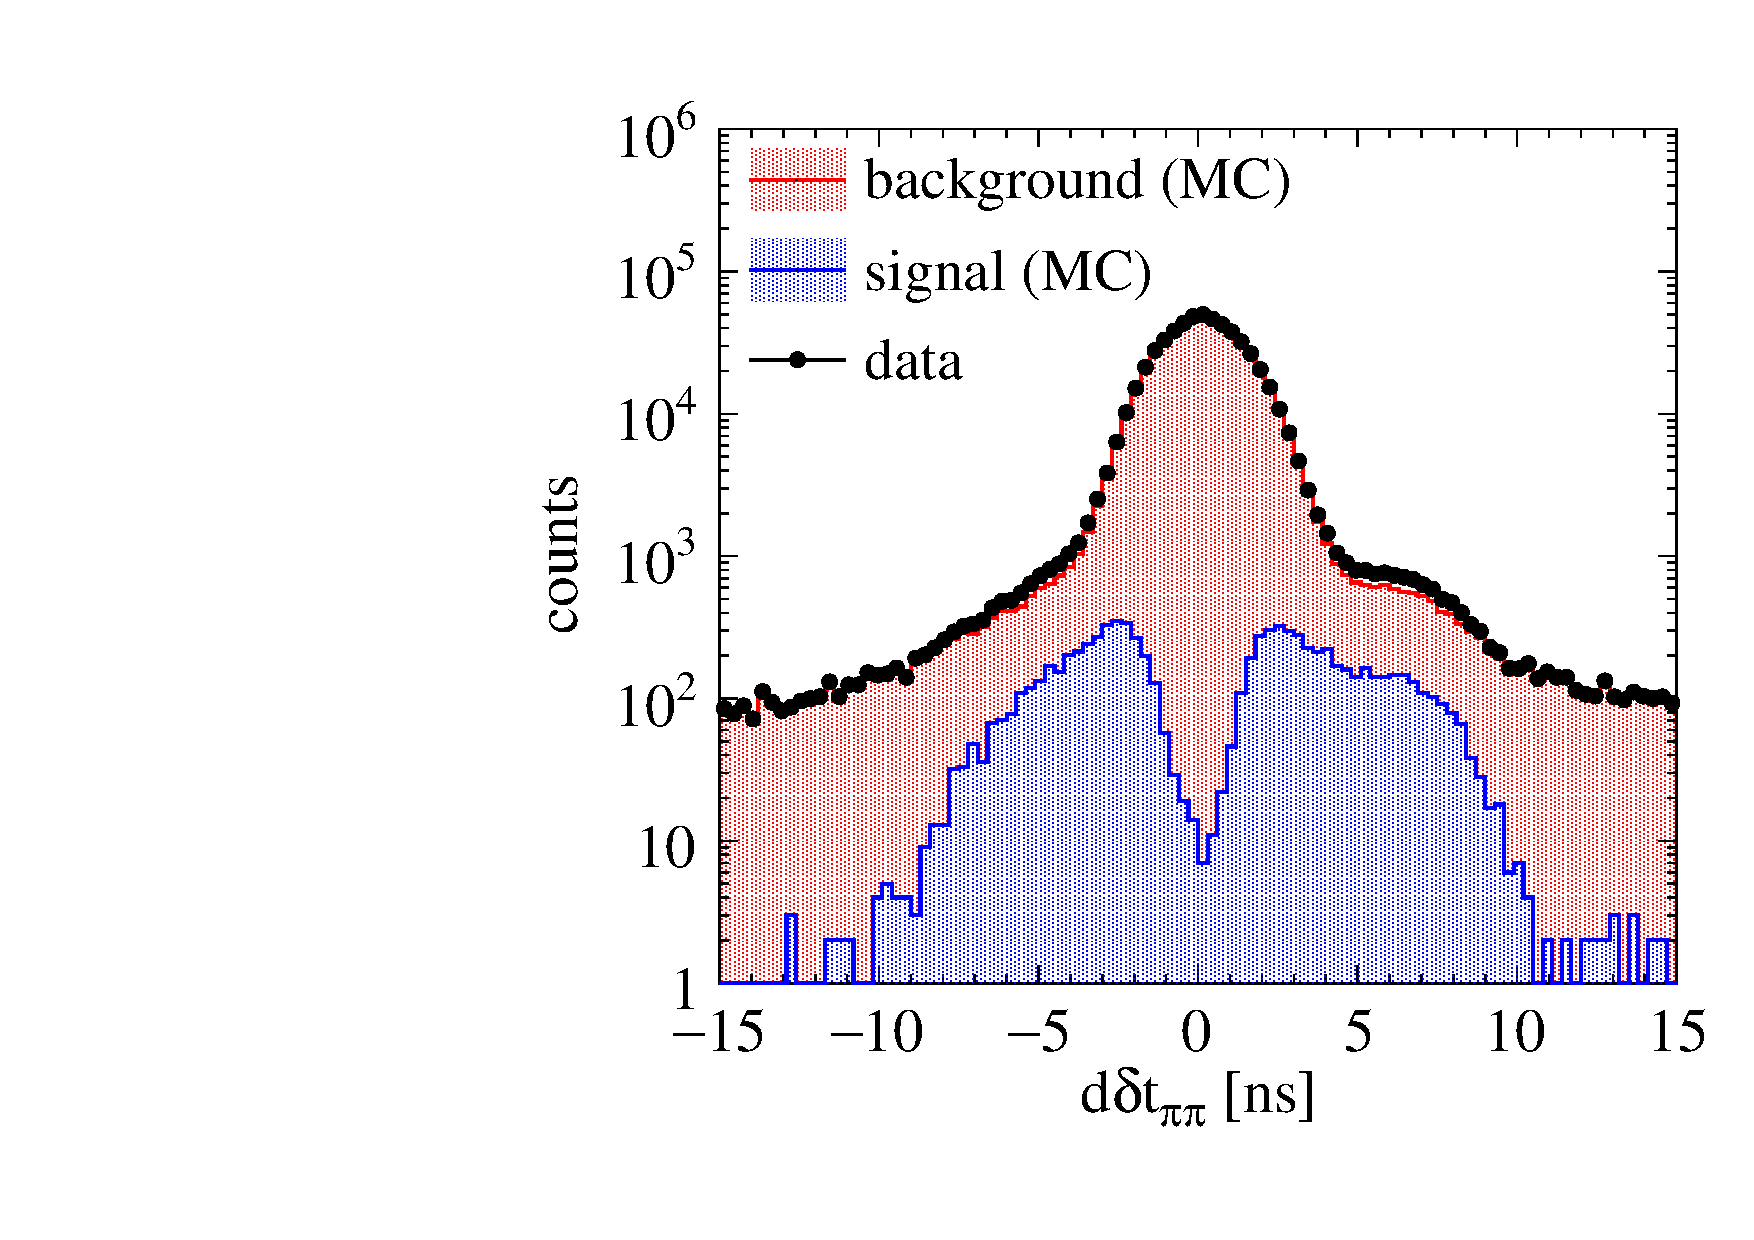
\includegraphics[width=0.45\textwidth]{Chapter7_analysis_kloe/img/tof1}};
    \draw[black, thick, dashed] (2.0,0.8) -- (2.0,4.0);
    \draw[black, thick, dashed] (3.55,0.8) -- (3.55,4.0);
    \draw[ultra thick, black!70!white, <->] (2.05, 1.2) -- (3.5, 1.2);
    \draw[black, thick, dashed] (4.1,0.8) -- (4.1,5.2);
    \draw[black, thick, dashed] (5.65,0.8) -- (5.65,5.46);
    \draw[ultra thick, black!70!white, <->] (4.15, 1.2) -- (5.6, 1.2);
  \end{tikzpicture}
  \caption{TOF discrepancy of two tracks with a $\pi^+\pi^-$ assumption. Dashed lines and gray arrows denote the two accepted regions.}\label{fig:tof_12_t1_1}
\end{figure}

Wrong assignment of particle mass hypotheses $x$ and $y$ can be revealed in the difference between $\delta t$ values for the two tracks (referred to as tracks 1 and 2) in an event:
\begin{equation}
  \label{eq:tof2_t1}
  d\delta t_{x,y} = \delta t_1(m_x) - \delta t_2(m_y),
\end{equation}
expected to vanish if both particles are correctly identified. Therefore, rejection of background is first performed with the distribution of $d\delta t_{\pi,\pi}$ for which both tracks are assumed to come from charged pions. As shown in~\fref{fig:tof_12_t1_1}, this distribution peaks at zero for the $\pi^+\pi^-$-dominated background while being shifted off zero for semileptonic events where one of the pion track assumptions is clearly incorrect. Events are accepted if they satisfy the following requirement:
\begin{equation*}
  |d\delta t_{\pi,\pi}| \in (1.5,\;10)\:\text{ns}.
\end{equation*}

\begin{figure}[h!]
  \centering
  \captionsetup[subfigure]{justification=centering}
  %
  \begin{subfigure}{0.45\textwidth}
  {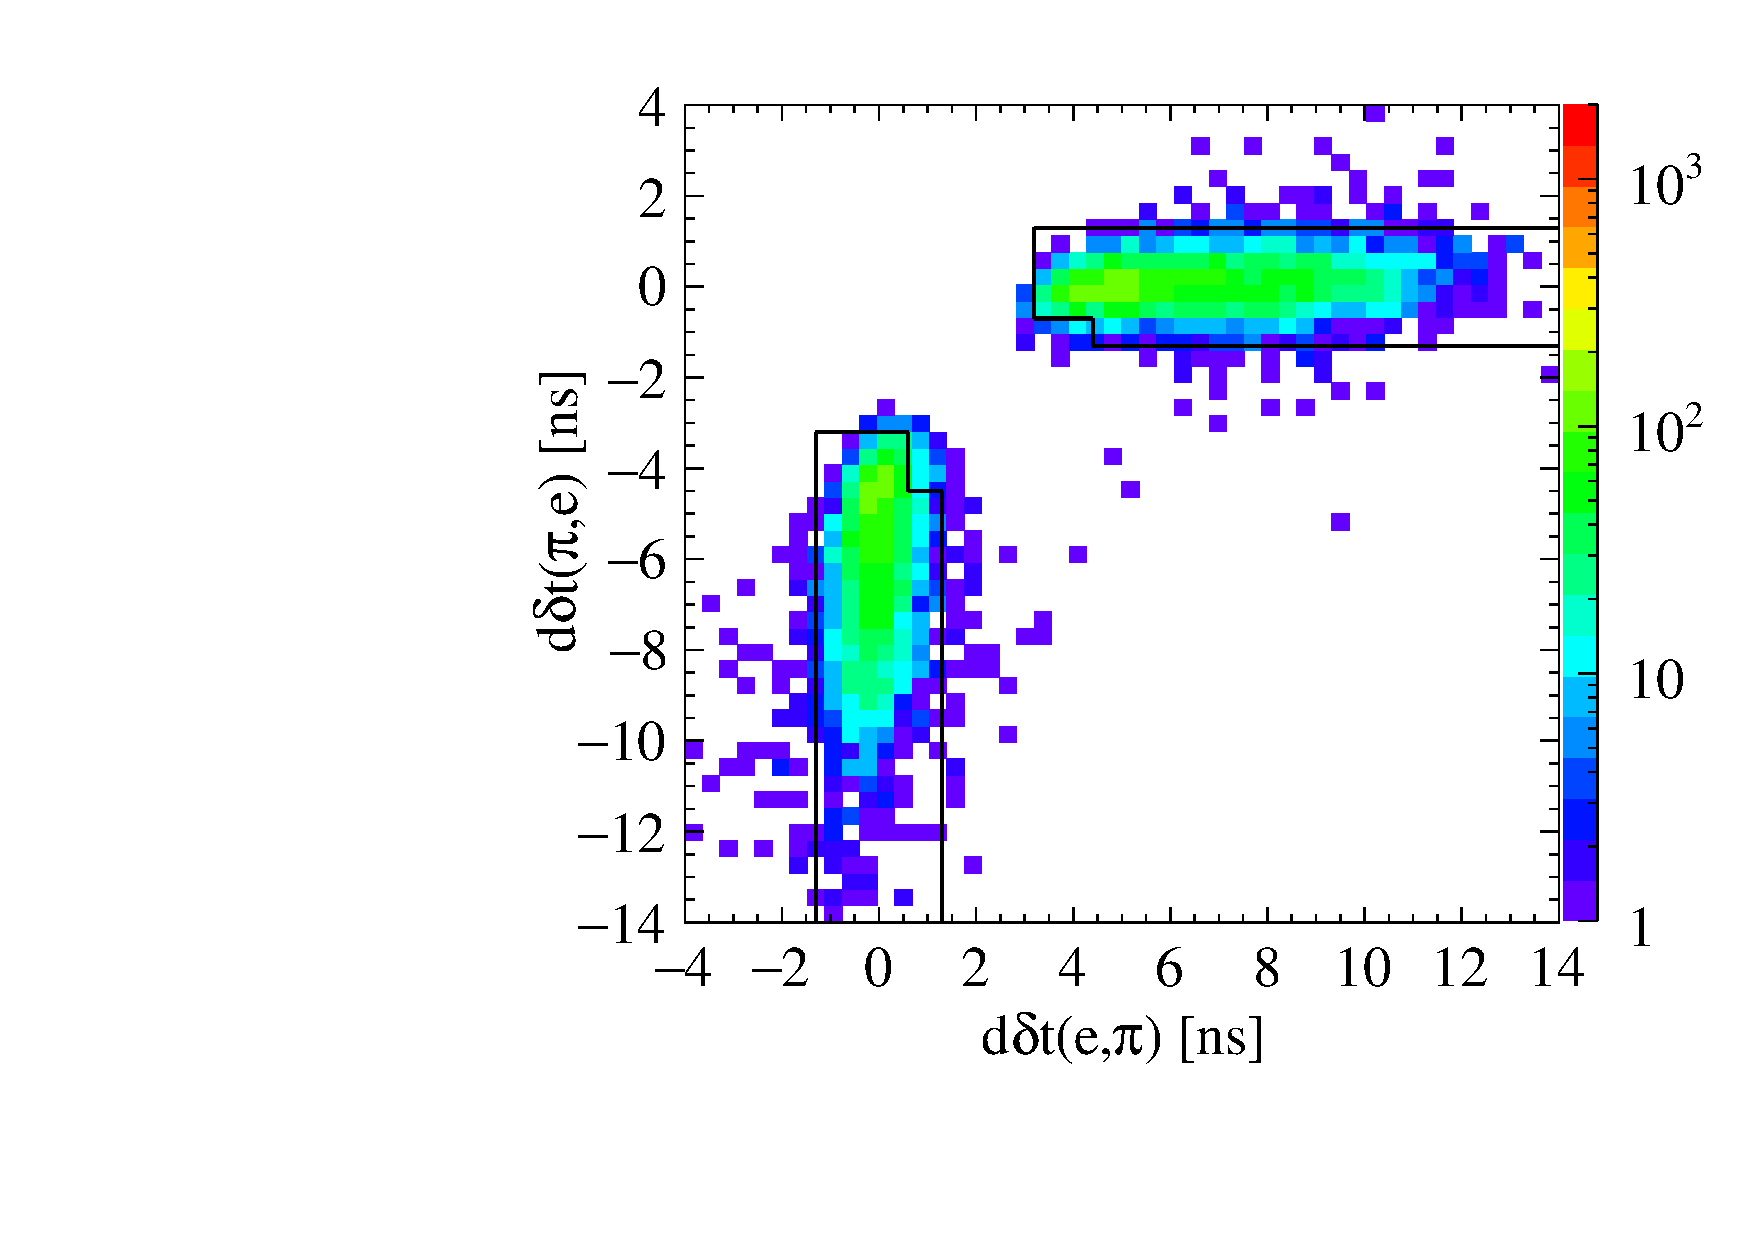
\includegraphics[width=1.0\textwidth]{Chapter7_analysis_kloe/img/tof2_signal}}
  \caption{Signal events (MC).}\label{fig:tof_12_t1_2}
\end{subfigure}
% 
  \hspace{1em}
\begin{subfigure}{0.45\textwidth}
  {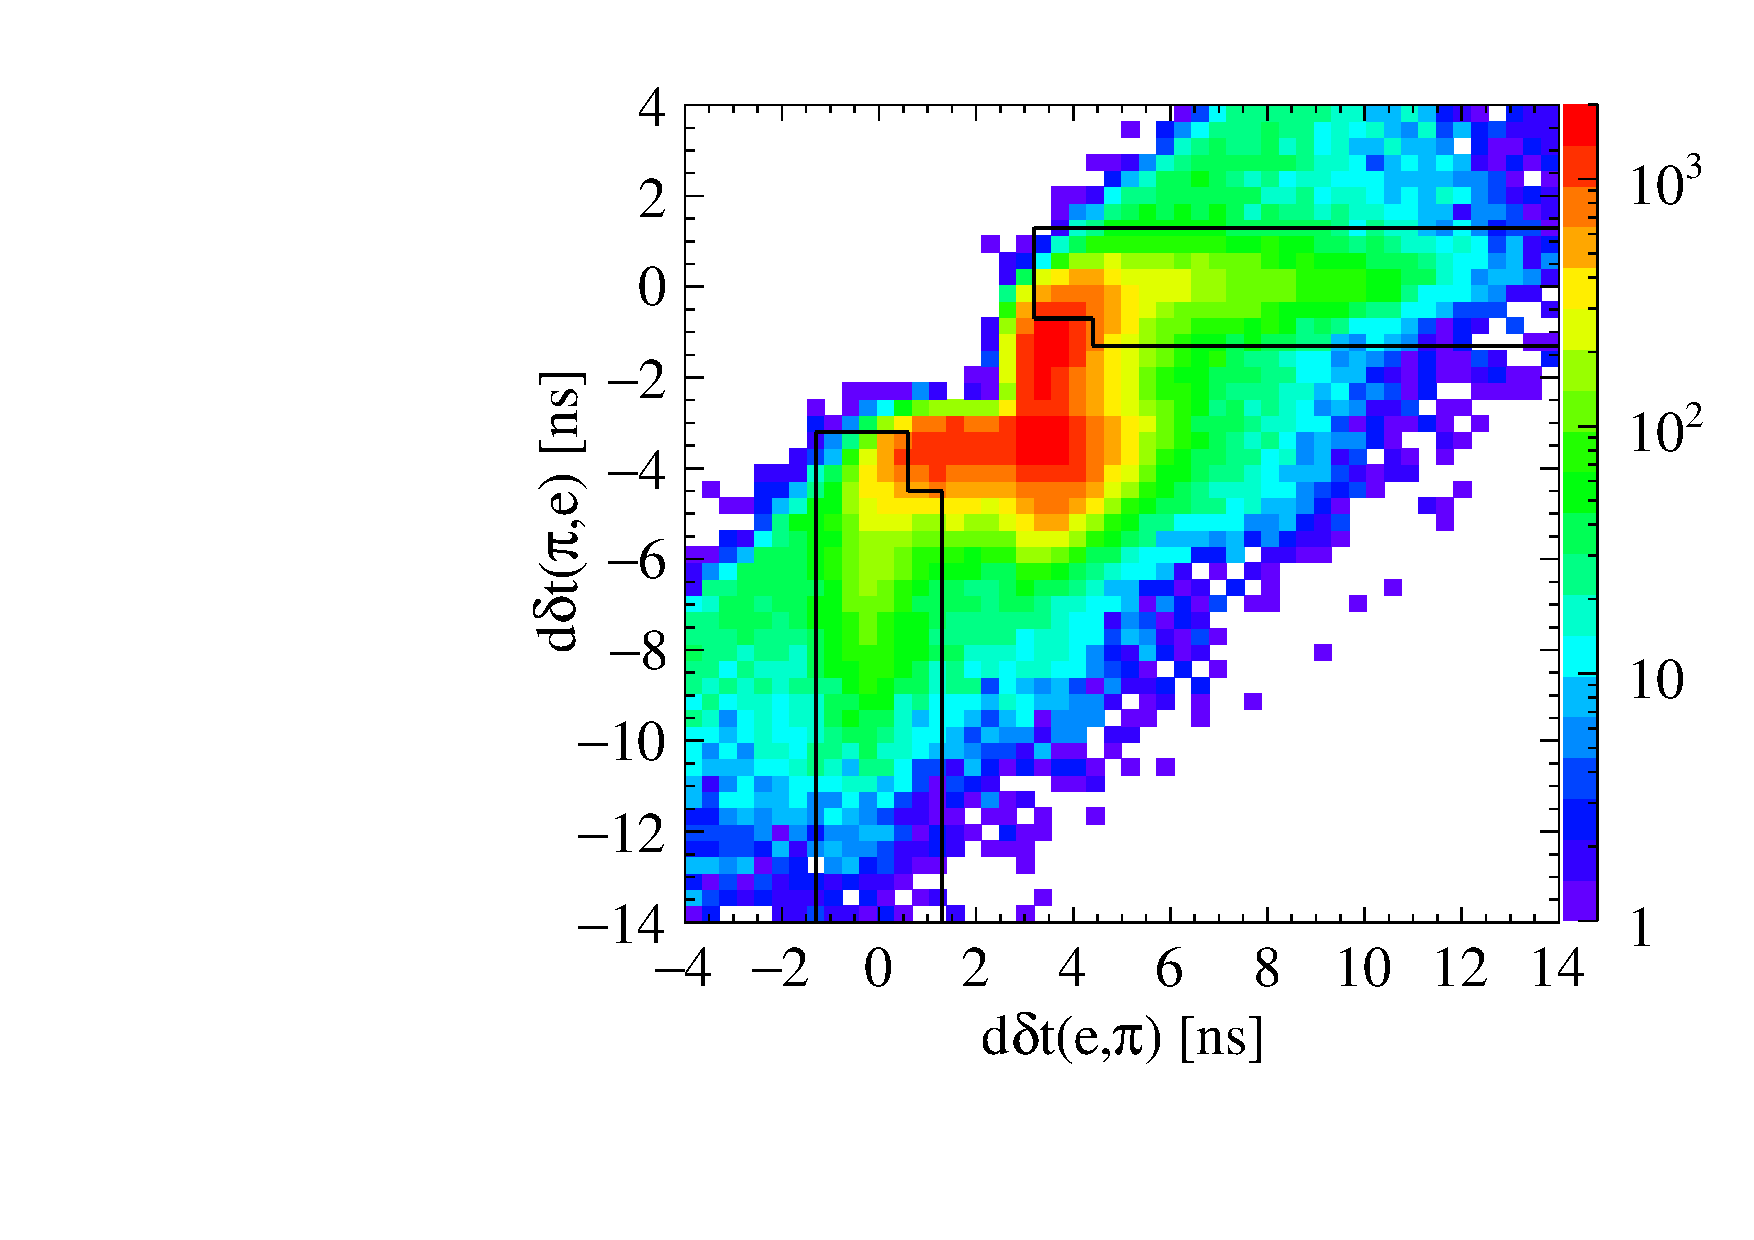
\includegraphics[width=1.0\textwidth]{Chapter7_analysis_kloe/img/tof2_background}}
  \caption{Background events (MC).}\label{fig:tof_12_t1_3}
  \end{subfigure}
%
  \begin{subfigure}{0.45\textwidth}
  {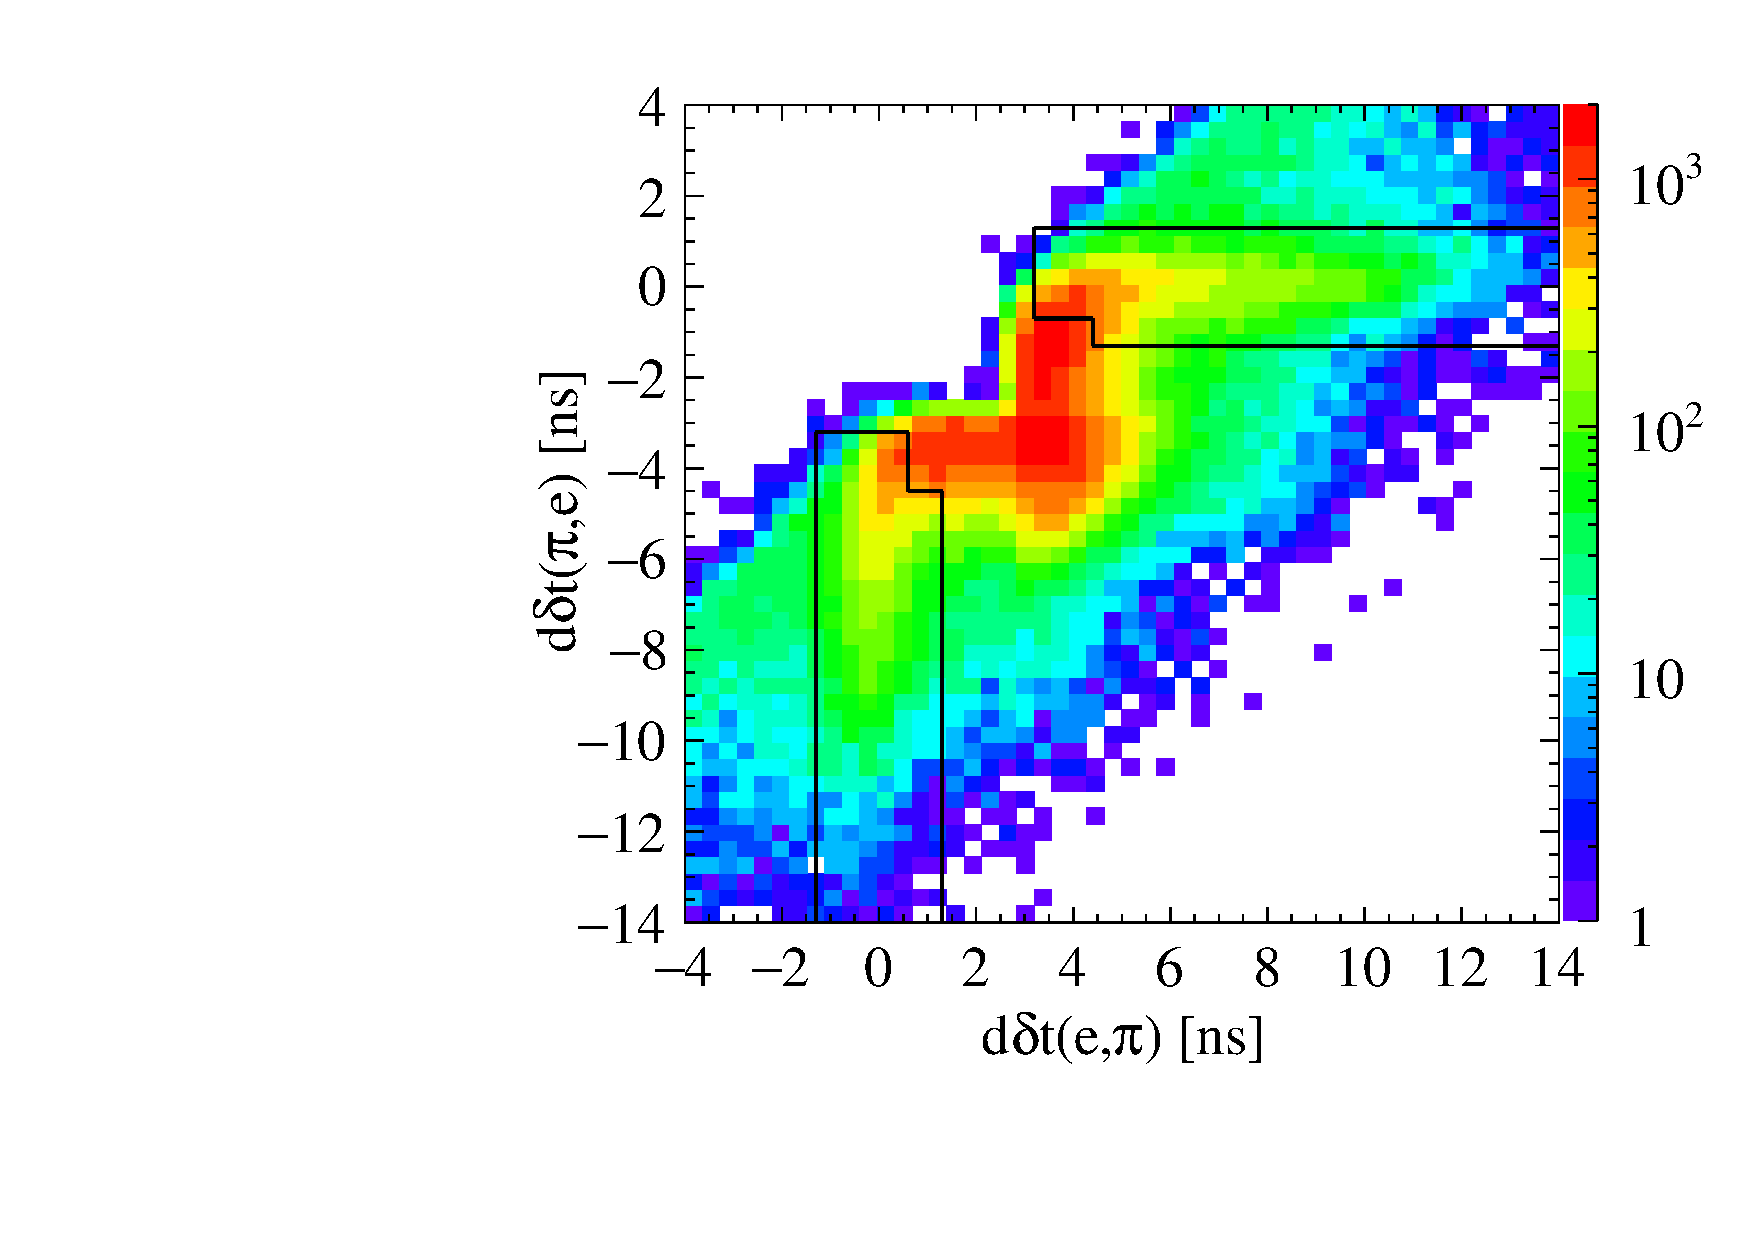
\includegraphics[width=1.0\textwidth]{Chapter7_analysis_kloe/img/tof2_data}}
  \caption{All data events.}\label{fig:tof_12_t1_4}
  \end{subfigure}
  % 
  \caption{Errors of two possible $\pi^{\pm}$ and $e^{\mp}$ mass hypotheses assignments to tracks. Solid lines denote accepted regions, each corresponding to one posible assignment of pion and electron mass hypotheses' assignment to the two DC tracks in an event.}\label{fig:tof_12_t1}
\end{figure}

Subsequently, an assignment of $\pi^{\pm}$ and $e^{\mp}$ mass hypotheses to the two tracks is tried in two possible configurations. The correct assignment is identified using the relative distributions of $d\delta t (\pi,e)$ and $d \delta t(e,\pi)$ presented in Figure~\ref{fig:tof_12_t1}. Signal events belong to one of two regions characterized by a small value of one of the $d\delta(x,y)$ discrepancies and significant value of the other one (marked with solid line in the figures). Affiliation to a particular region indicates the correct attribution of pion and electron masses to each of the tracks. Background events, on the other hand, mostly populate the region closer to diagonal where both $d\delta t(\pi,e)$ and $d\delta t(e,\pi)$ are non-zero. Consequently, events are selected for further analysis if they belong to one of the regions marked with solid line in Figure~\ref{fig:tof_12_t1}.
%
% TODO: wypisac explicite wartosci ciec
%

\subsection{Correction of event start time}\label{sec:t0_corr}
%
% TODO: dopisac, ze standardowe T0 nie dziala bo nie ma prompt fotonow w zdarzeniu
%
\begin{figure}[b]
  \centering
  \begin{subfigure}{0.45\textwidth}
  {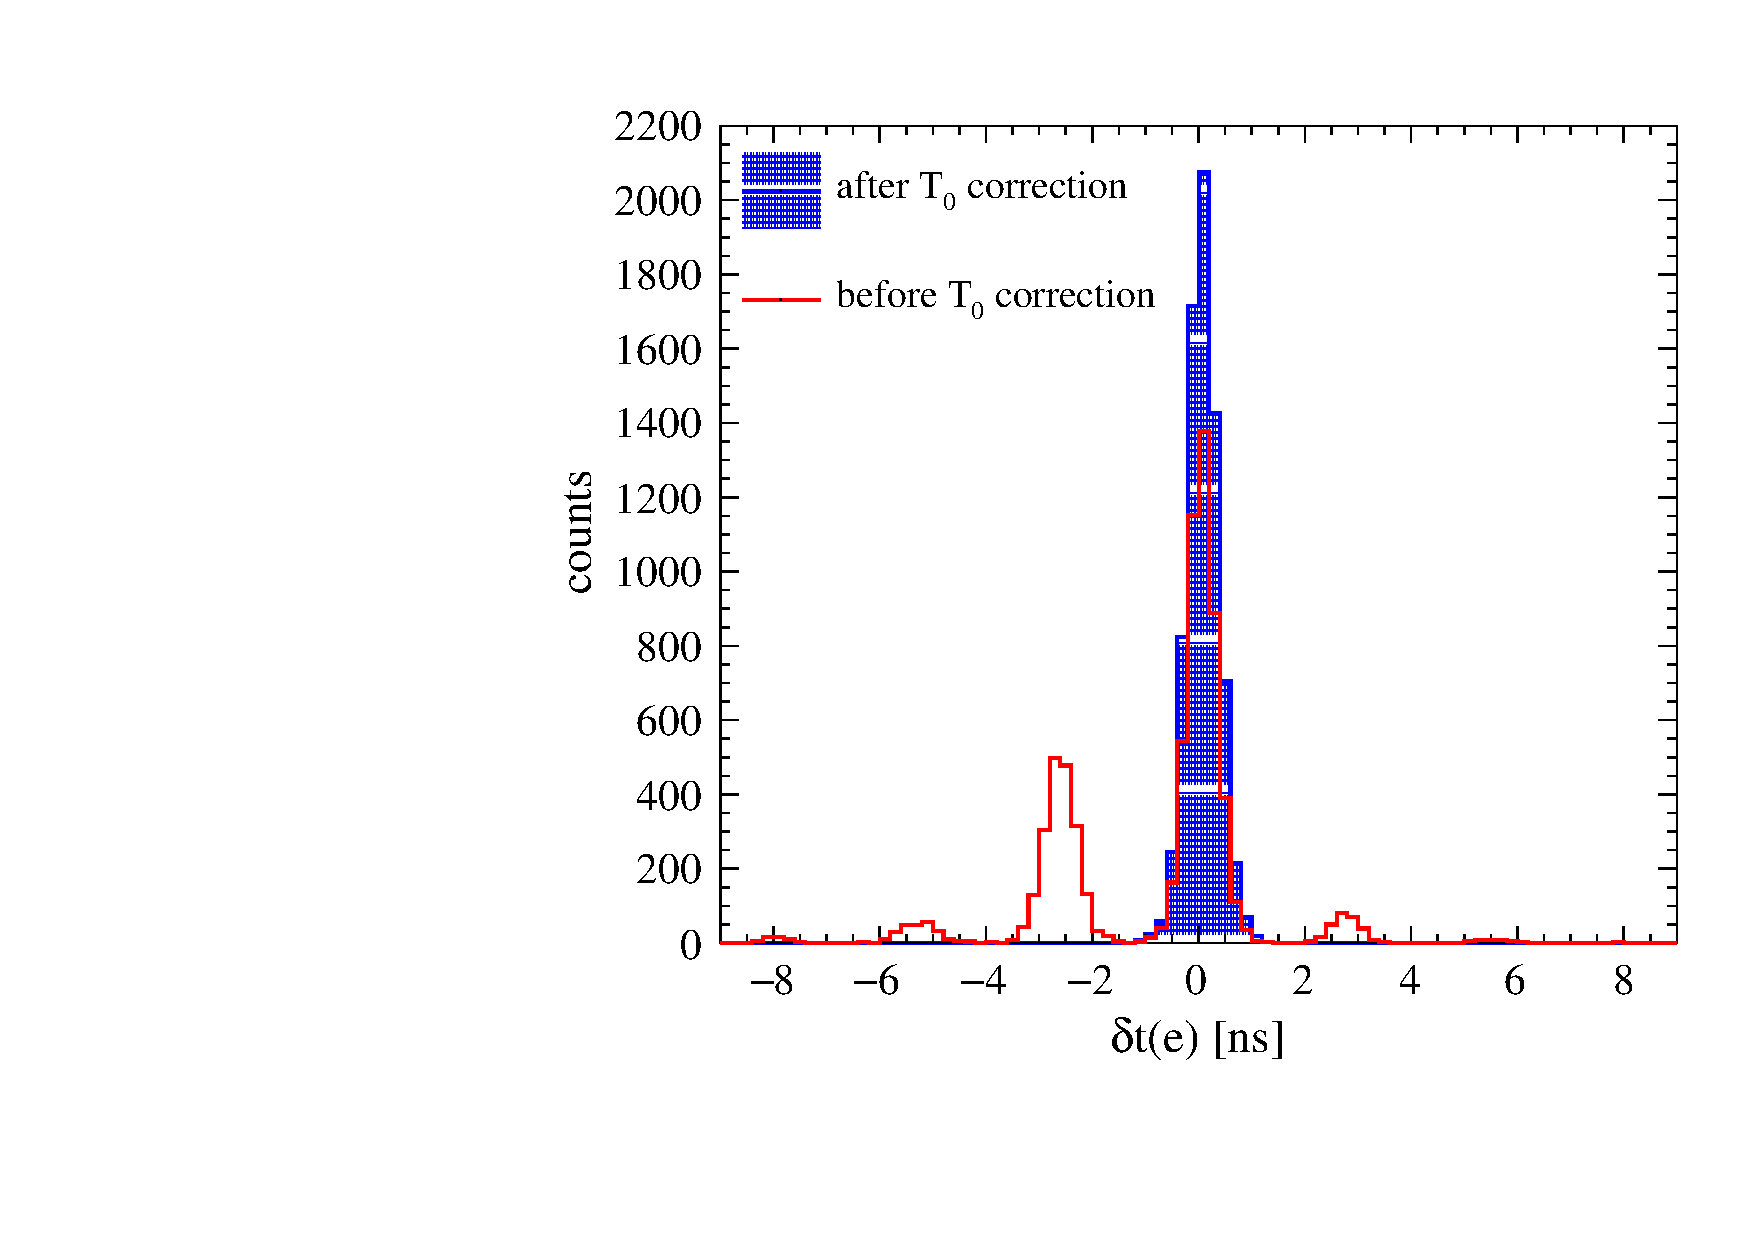
\includegraphics[width=1.0\textwidth]{Chapter7_analysis_kloe/img/tof_e_t0}}
\end{subfigure}
%
\begin{subfigure}{0.45\textwidth}
  {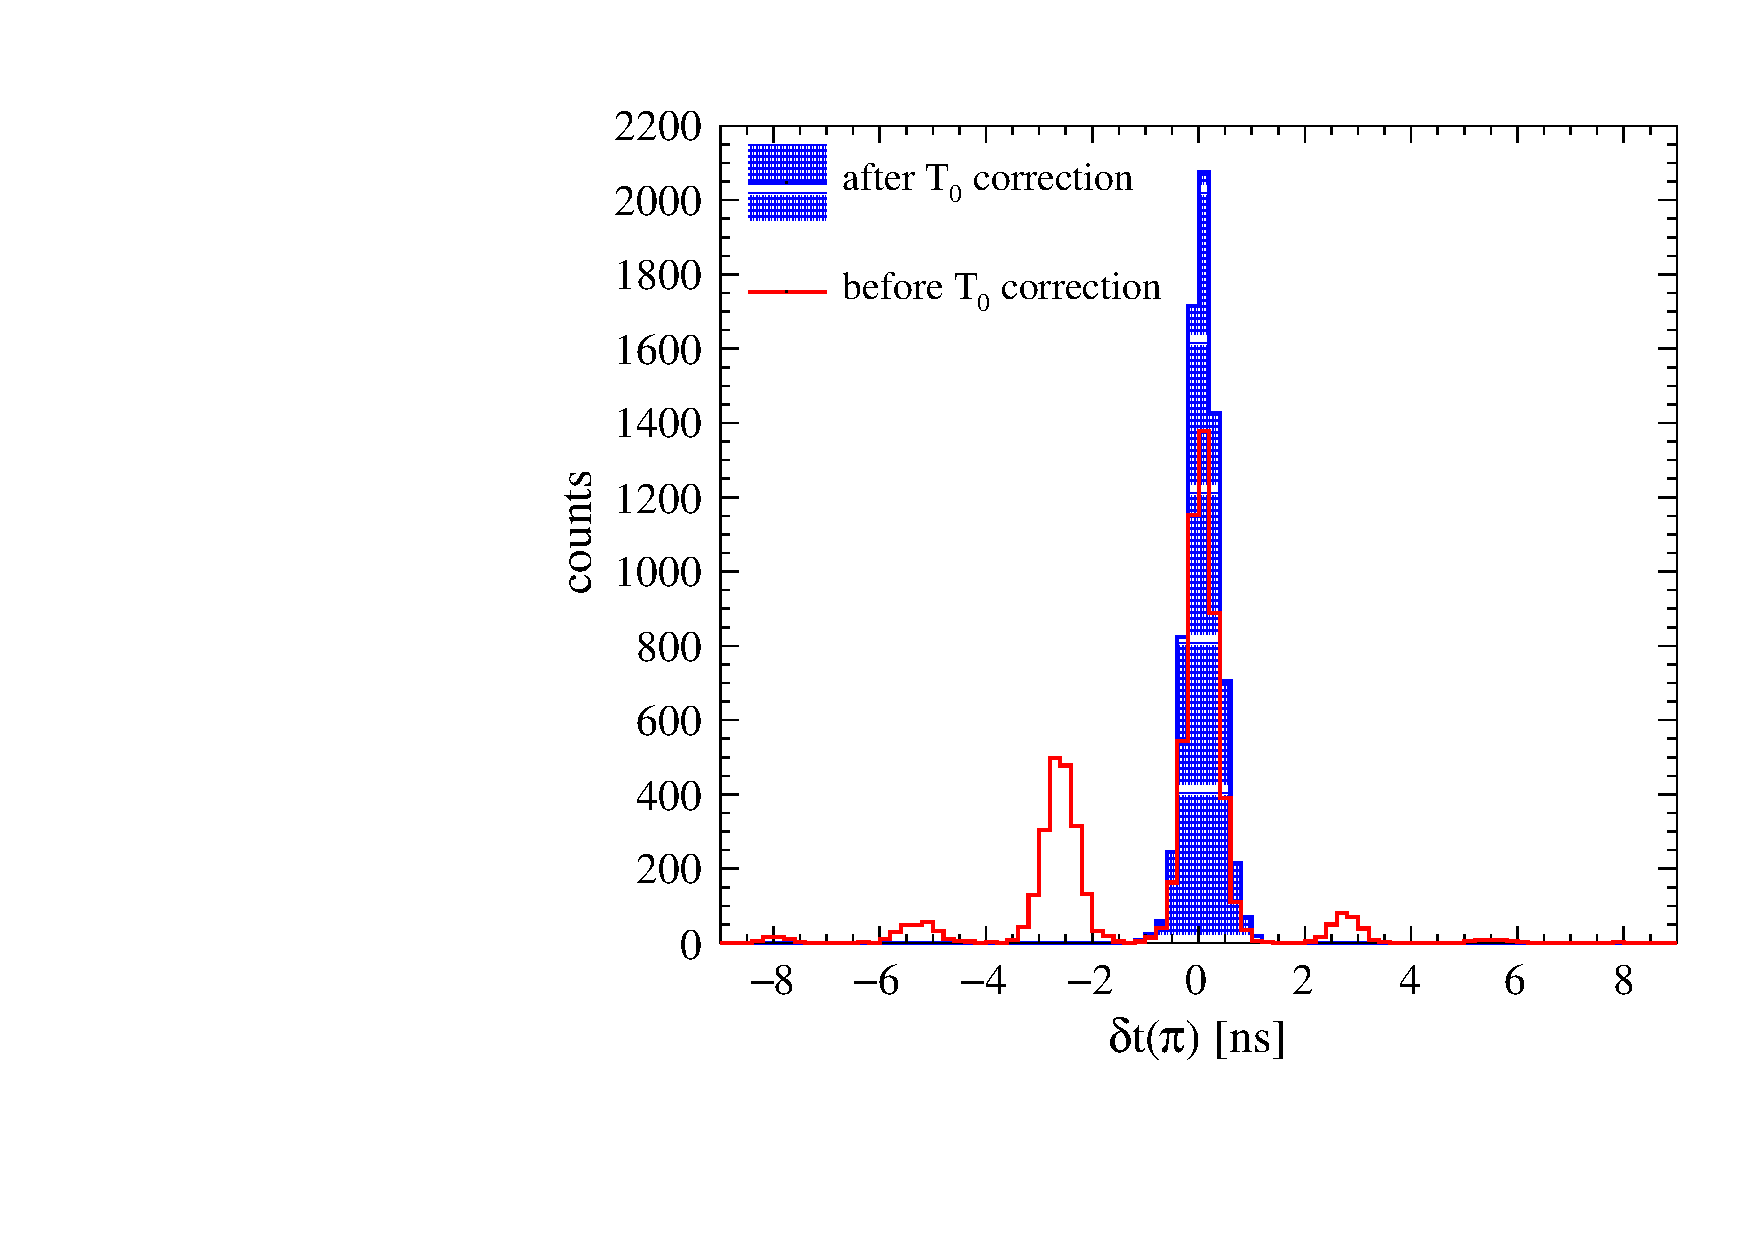
\includegraphics[width=1.0\textwidth]{Chapter7_analysis_kloe/img/tof_pi_t0}}
\end{subfigure}
%
\begin{subfigure}{0.45\textwidth}
  {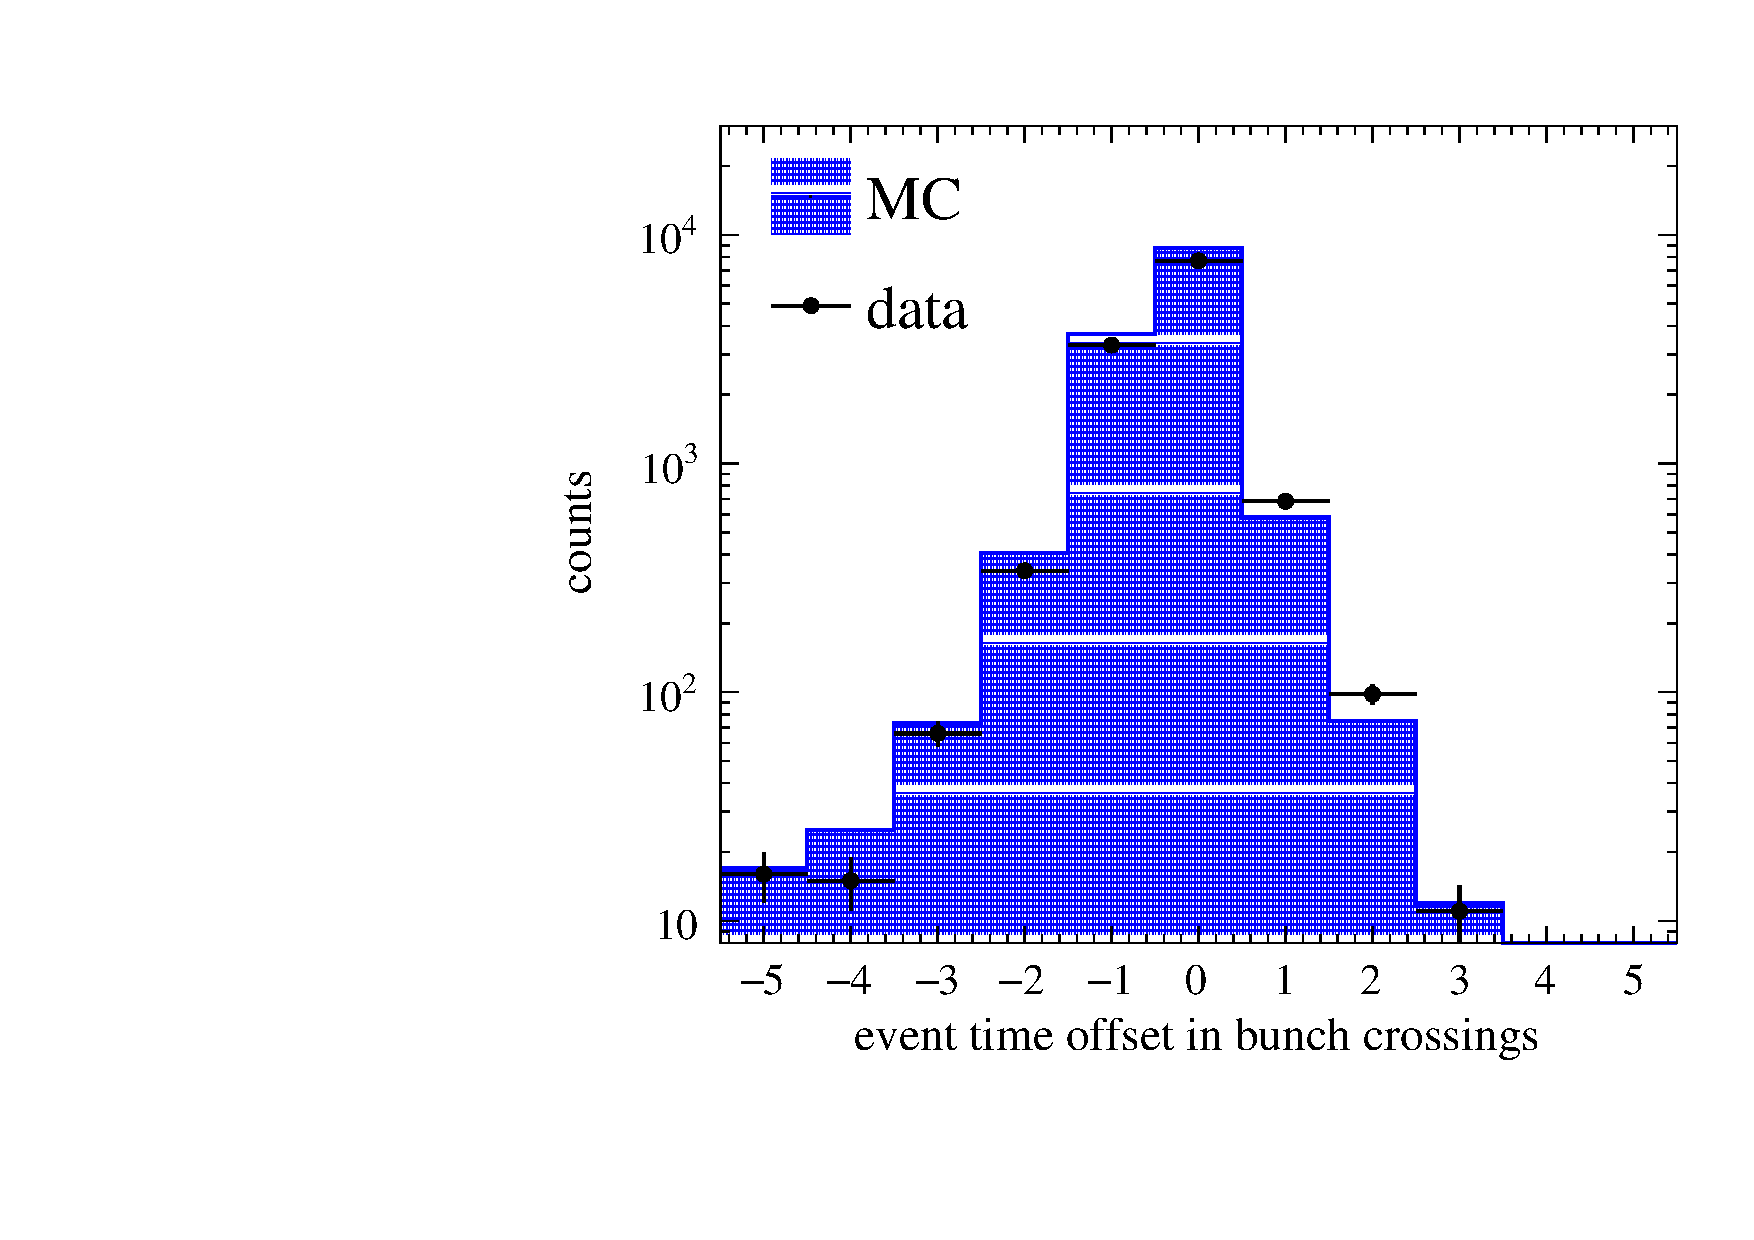
\includegraphics[width=1.0\textwidth]{Chapter7_analysis_kloe/img/t0_bunches}}
\end{subfigure}
  \caption{Top: discrepancies between recorded and expected time of flight for the track identified as originating from $e^{\pm}$ (left) and $\pi^{\mp}$ (right) before and after correction of event $T_0$. Distributions were obtained with data. For clarity, the  presented distributions were obtained after the background rejection steps discussed in~\sref{sec:t1-fine-selection} to avoid contamination from incorrectly identified tracks. Bottom: number of collider bunch crossing periods shifted as a result of event $T_0$ correction, for data and MC simulations.}\label{fig:t0_corr}
\end{figure}

Once the tracks originating from pion and electron/positron are identified, their TOF calculated with correct mass hypotheses can be used to determine a correction to the event start time which is later subtracted from all times recorded in the event. If the discrepancies between recorded and expected time of flight for the pion and lepton (compare~\eref{eq:dtof_t1}) are denoted as $\delta t(\pi)$ and $\delta t(e)$ respectively, the correction to event $T_0$ is obtained as an average of these values for both tracks, rounded to a multiple of DA$\Phi$NE bunch crossing periods $T_{RF}$~(compare~\eref{eq:t0_prompt}):
\begin{equation}
  \label{eq:t0_correction_semil}
  T'_{0} = T_{RF}\cdot nint\left(\frac{\delta t(\pi) + \delta t(e)}{2T_{RF}}\right).
\end{equation}

\fref{fig:t0_corr} shows the distributions of $\delta t(\pi)$ and $\delta t(e)$ for each of the charged particles in an event, before and after application of the $T_0$ correction the recorded times of EMC clusters. The uncorrected cluster times are most commonly offset forward by one bunch crossing, i.e.\ by 2.72~ns resulting in several peaks of the $\delta t$ distributions. The bottom panel of~\fref{fig:t0_corr} presents the total number of bunch crossings which needed to be shifted in an event. The $T_0$ correction is required in about \SI{32}{\percent} of the considered events.

\subsection{Fine selection of $\Ks\to\pi e\nu$ decays}\label{sec:t1-fine-selection}
With a correct event start time, the TOF discrepancies $\delta t(\pi)$ and $\delta t(e)$ are concentrated around zero for both the pion and electron/positron tracks~(see~\fref{fig:tof3_cut}\subref{fig:tof3_cut_1}). On the other hand, background events in which at least one of the particles was incorrectly identified must be shifted off the center of the distributions presented in~\fref{fig:tof3_cut}. In fact, the shift is usually exhibited by both values as the error in calculation of one of $\delta t(\pi)$ or $\delta t(e)$ is eventually propagated to both through an incorrect event $T_0$ value subtracted from EMC cluster times.

\begin{figure}[h!]
  \centering
\captionsetup[subfigure]{justification=centering}
  \begin{subfigure}{0.45\textwidth}
    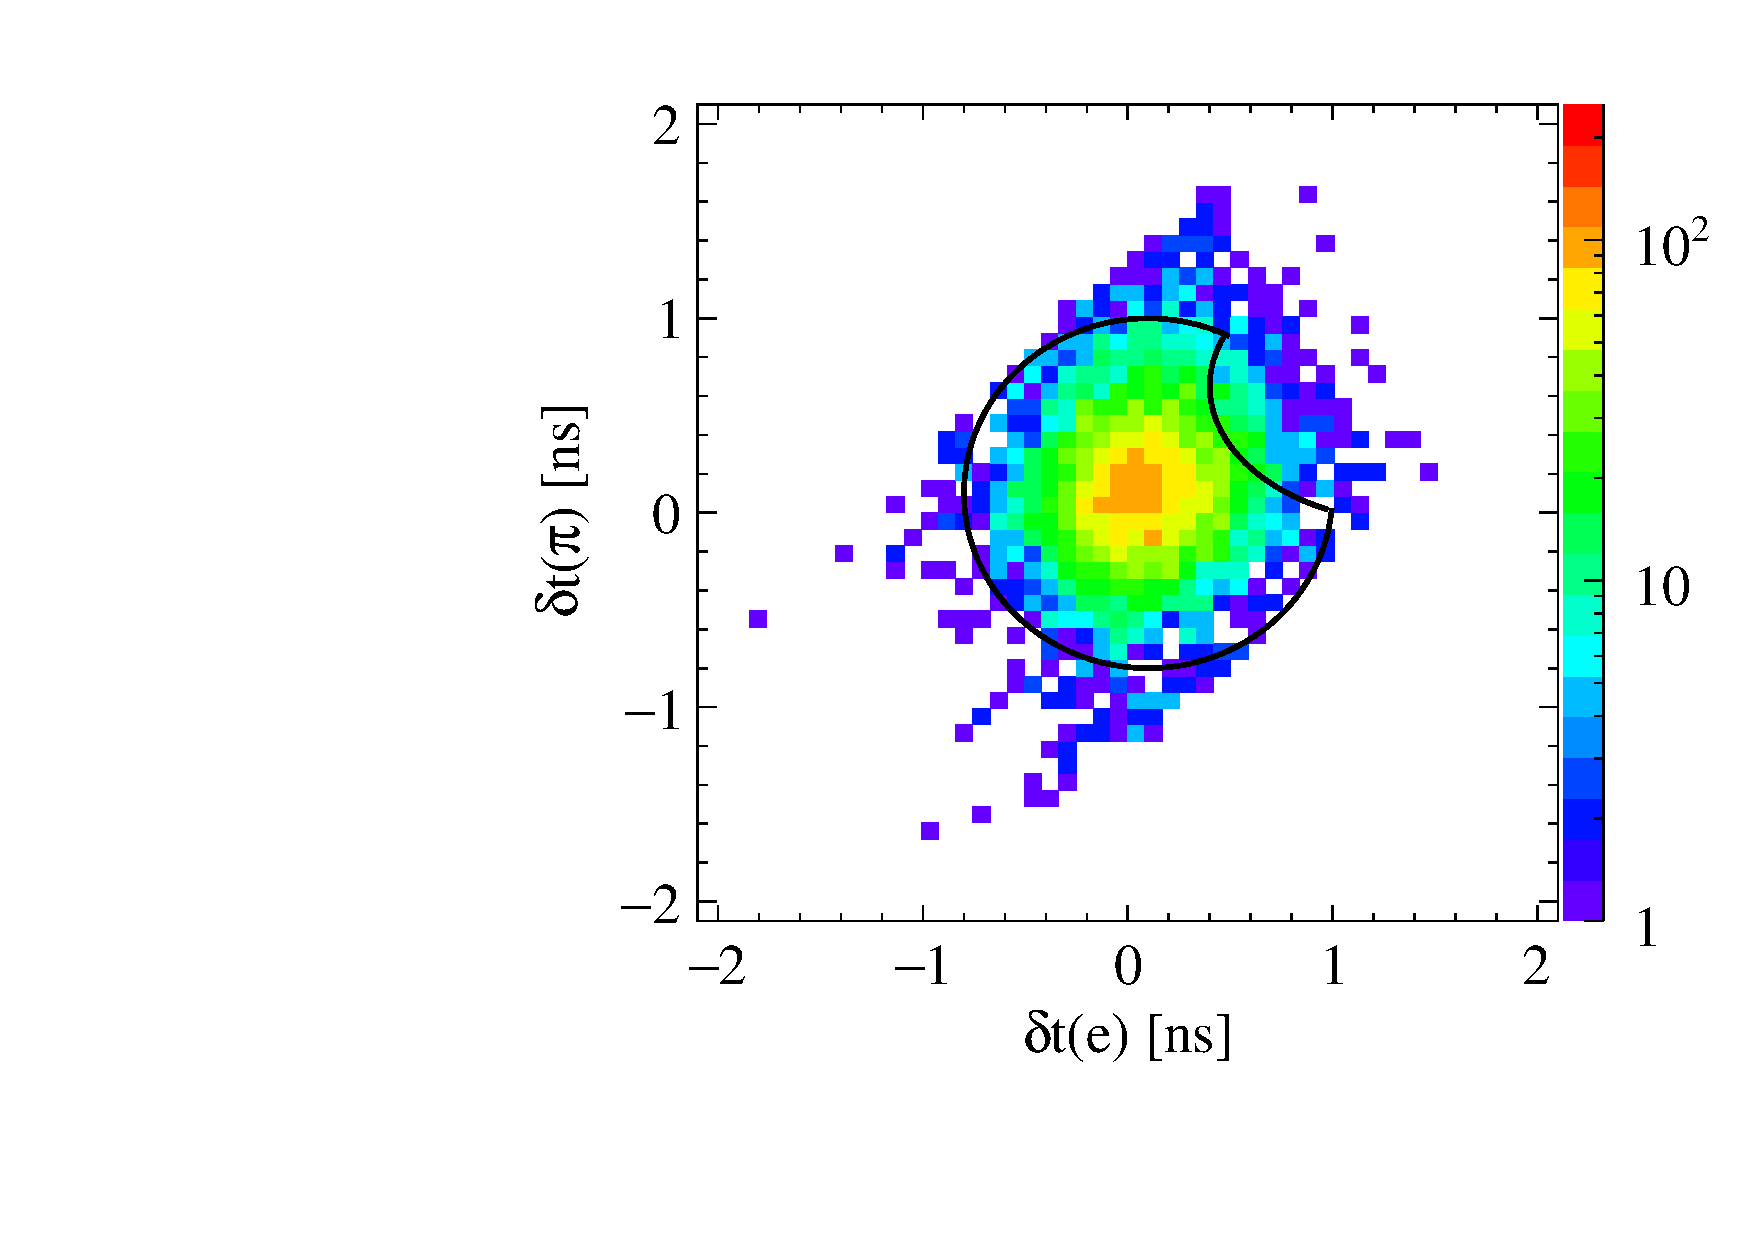
\includegraphics[width=1.0\textwidth]{Chapter7_analysis_kloe/img/tof3_signal}
    \caption{Signal events (MC)}\label{fig:tof3_cut_1}
  \end{subfigure}
  %
  \begin{subfigure}{0.45\textwidth}
    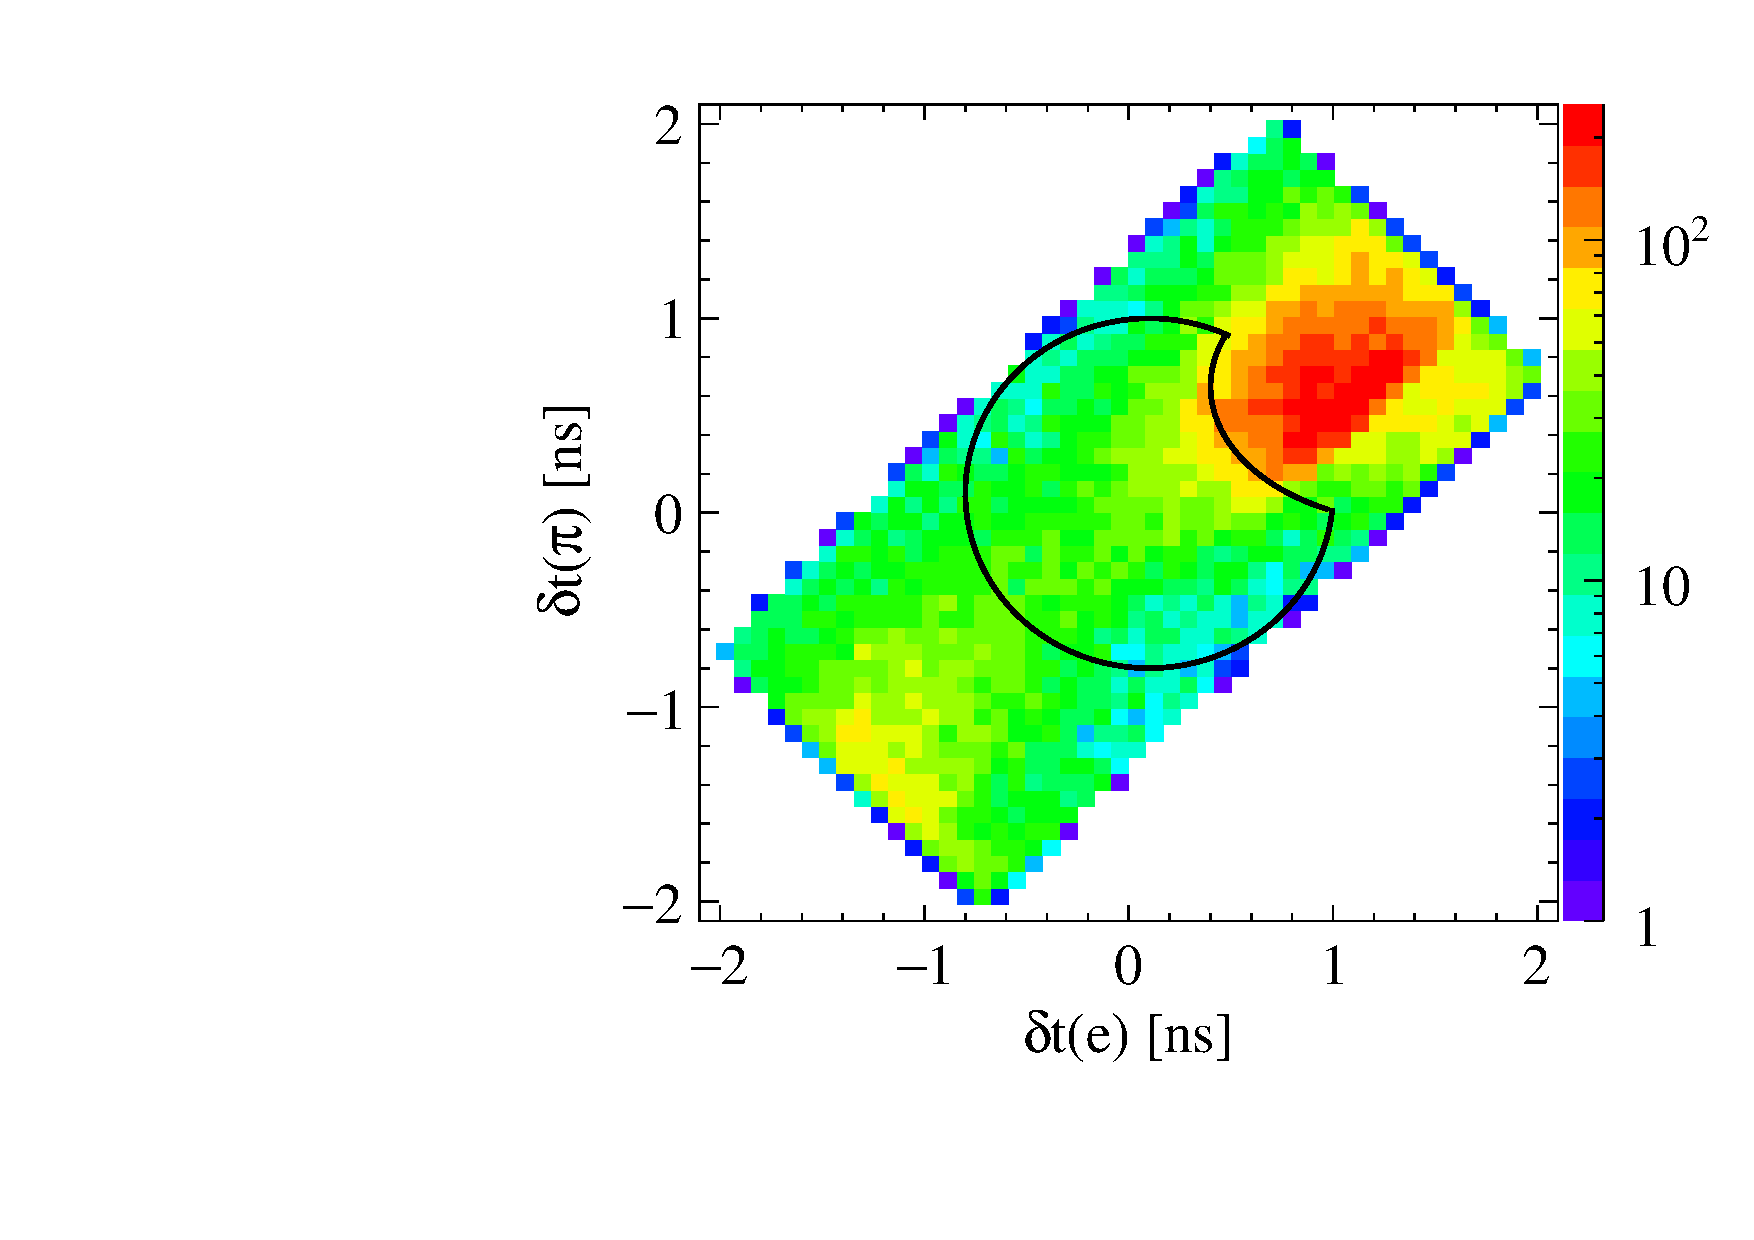
\includegraphics[width=1.0\textwidth]{Chapter7_analysis_kloe/img/tof3_background}
    \caption{Background events (MC)}
  \end{subfigure}
  %
  \begin{subfigure}{0.45\textwidth}
    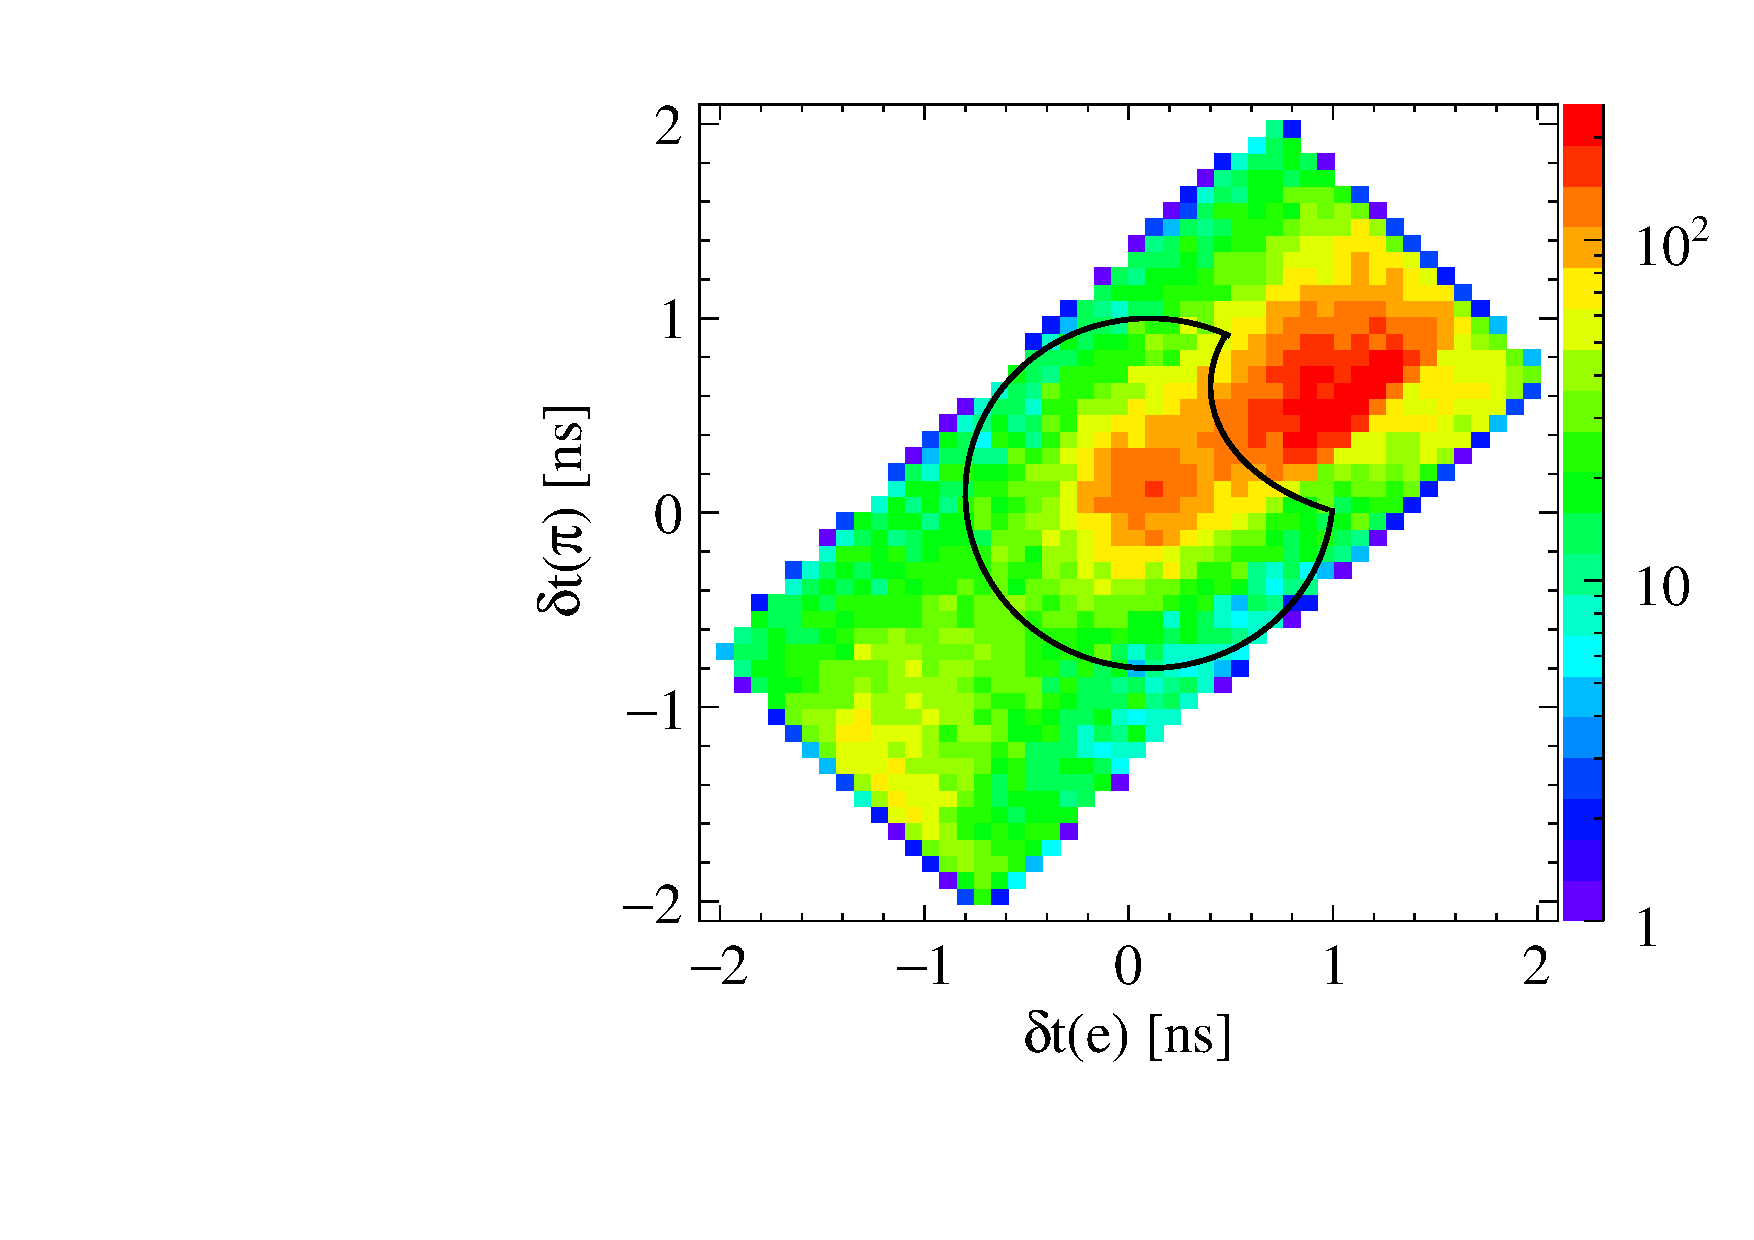
\includegraphics[width=1.0\textwidth]{Chapter7_analysis_kloe/img/tof3_data}
    \caption{All data events}
  \end{subfigure}
  \caption{Relative distribution of TOF discrepancies for tracks identified as pion and electron/positron. Limits of the populated region result from cuts introduced at a previous stage of the TOF analysis~(see~\fref{fig:tof_12_t1}). Events are retained if they lie inside the region marked with black solid line.}\label{fig:tof3_cut}
\end{figure}

Therefore, the relative distribution of both TOF discrepancies from~\fref{fig:tof3_cut} is useful for rejection of background form non-semileptonic decays of $\Ks$ which is concentrated in the top upper part of the distributions. To achieve the best purity of $\Ks\to\pi e \nu$ events, only events lying inside a circle in the center of the distribution are kept for further analysis, with exception of those lying in a ellipse surrounding the background region, i.e.:
\begin{eqnarray*}
  \label{eq:tof_cut_3}
  \left(\frac{\delta t(\pi)-0.1\:\text{ns}}{0.9\:\text{ns}}\right)^2 &+& \left(\frac{\delta t(e)-0.1\:\text{ns}}{0.9\:\text{ns}}\right)^2 < 1\\
  &\land&\\
  {\left(\frac{\delta t(\pi)-0.65\:\text{ns}}{0.7\:\text{ns}}\right)}^2 &+& {\left(\frac{\delta t(e)-1.4\:\text{ns}}{1.0\:\text{ns}}\right)}^2 > 1,
\end{eqnarray*}
as marked with the black line in~\fref{fig:tof3_cut}.

After the two-dimensional cut on the $\delta t$ values, a majority of the surviving background comes from three classes:
\begin{itemize}
\item $\Ks\to\pi^+\pi^-$ with imperfectly reconstructed tracks where wrong momentum estimation for one of the pions allows it to pass the selection criteria for an electron/positron track,
\item radiative $\Ks\to\pi^+\pi^-\gamma$ decays where a photon carries away a part of the momentum,
\item $\Ks\to\pi^+\pi^-\to \pi\mu\nu$ decay chains where one of the charged pions decayed into a muon and a neutrino before the inner wall of the KLOE drift chamber so that its decay was not recorded.
\end{itemize}
Since the decay vertices located close to the beamline and thus not inside the drift chamber are reconstructed using extrapolations of tracks from the DC towards the $\phi$ decay point, in the $\Ks\to\pi^+\pi^-\to \pi\mu\nu$ case one of the recorded tracks in fact corresponds to a muon not originating at the same vertex as the pion track as depicted schematically in~\fref{fig:kspimu}.

\begin{figure}[h!]
  \centering
  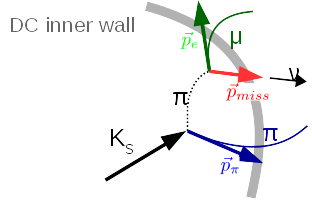
\includegraphics[width=0.4\textwidth]{Chapter7_analysis_kloe/img/kspimu}
  \caption{Scheme of a $\Ks\to\pi^+\pi^-\to \pi\mu\nu$ decay occurring before the inner wall of the KLOE drift chamber so that the muon track is misidentified as electron or positron and extrapolated to an artificial vertex common with the pion track.}\label{fig:kspimu}
\end{figure}

To recognize such events, each of the two tracks is extrapolated backwards to its point of closest approach (PCA) to the average $\phi$ vertex. If their distances of closest approach to $\phi$ measured in the $xy$ plane of the detector are denoted as $d_{xy}(\pi)$ and $d_{xy}(e)$, the following variable:
\begin{equation}
  \label{eq:dpca}
  d_{PCA} = d_{xy}(e) - d_{xy}(\pi),
\end{equation}
is sensitive to tracks not originating at the same $\Ks$ decay vertex as in the case of muon track from $\Ks\to\pi^+\pi^-\to \pi\mu\nu$. For the tracks from $\Ks\to\pi e\nu$ originating close to the primary vertex, the $d_{PCA}$ distribution peaks around zero as shown in~\fref{fig:dpca_de_cut}. To enhance the background discrimination power of this variable, it was correlated with a difference between missing energy and missing momentum in a decay defined as:
\begin{equation}
  \label{eq:de_pi_e}
  \Delta E(\pi,e) = E_{miss}(\pi,e) - p_{miss} = E_{K_S}-E_{\pi}-E_{e} - |\vec{p}_{K_S}-\vec{p}_{\pi}-\vec{p}_{e}|,
\end{equation}
where the energies of tracks identified as pion and electron/positron are calculated using respective particle mass hypotheses~\cite{Ambrosino:2006si,daria_memo}. This value is sensitive to all three background components listed above as the electron mass hypothesis is wrong for one of the tracks in such events. For signal events, $\Delta E(\pi,e)$ is expected to be close to zero. Although the resolution of $\Delta E(\pi,e)$ in case of the considered process $\Ks\Kl\to \pi e \nu\;3\pi^0$ is limited due to imperfect knowledge of the decaying $\Ks$ momentum, the two dimensional distributions of $d_{PCA}$ relative to $\Delta E(\pi,e)$ presented in~\fref{fig:dpca_de_cut} exhibit the background components clustered in an off-center region. Events are selected if they lie within the marked rhombus and outside an ellipse enclosing the background-populated area, which is equivalent to the following conditions:
\begin{eqnarray*}
  d_{PCA}/\text{cm} &<& -0.1\cdot\Delta E(\pi,e)/\text{MeV}+5, \\
  d_{PCA}/\text{cm} &>&  0.06\cdot\Delta E(\pi,e)/\text{MeV}-3, \\
  d_{PCA}/\text{cm} &>& -0.06\cdot\Delta E(\pi,e)/\text{MeV}-3, \\
  d_{PCA}/\text{cm} &<& 0.1\cdot\Delta E(\pi,e)/\text{MeV}+5, \\
  \left(\frac{d_{PCA}-2.8\:\text{cm}}{3.4\:\text{cm}}\right)^2 &+& \left(\frac{\Delta E(\pi,e)-27\:\text{MeV}}{16.7\:\text{MeV}}\right)^2 > 1.
\end{eqnarray*}

\begin{figure}[h!]
  \centering
\captionsetup[subfigure]{justification=centering}
  \begin{subfigure}{0.45\textwidth}
    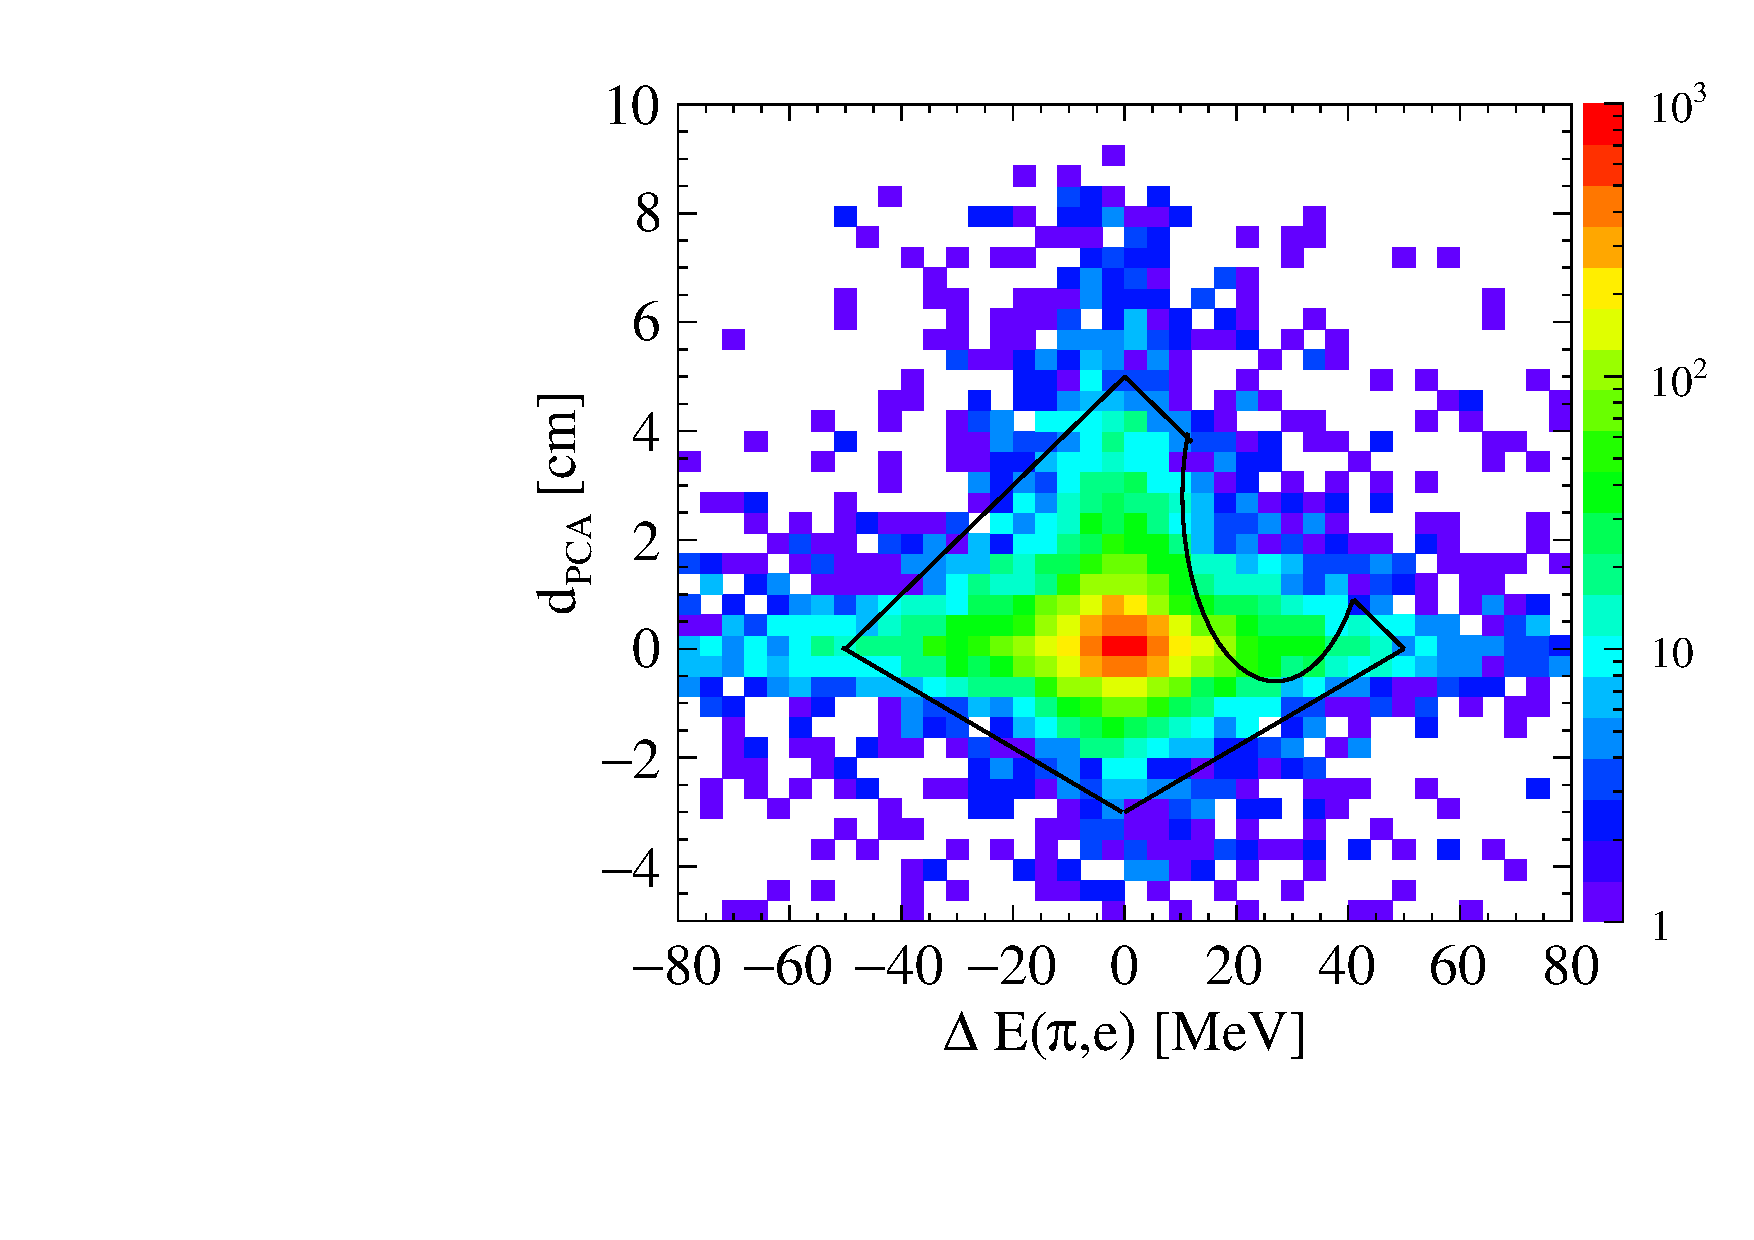
\includegraphics[width=1.0\textwidth]{Chapter7_analysis_kloe/img/dpca_de_signal}
    \caption{Signal events (MC)}
  \end{subfigure}
  %
  \begin{subfigure}{0.45\textwidth}
    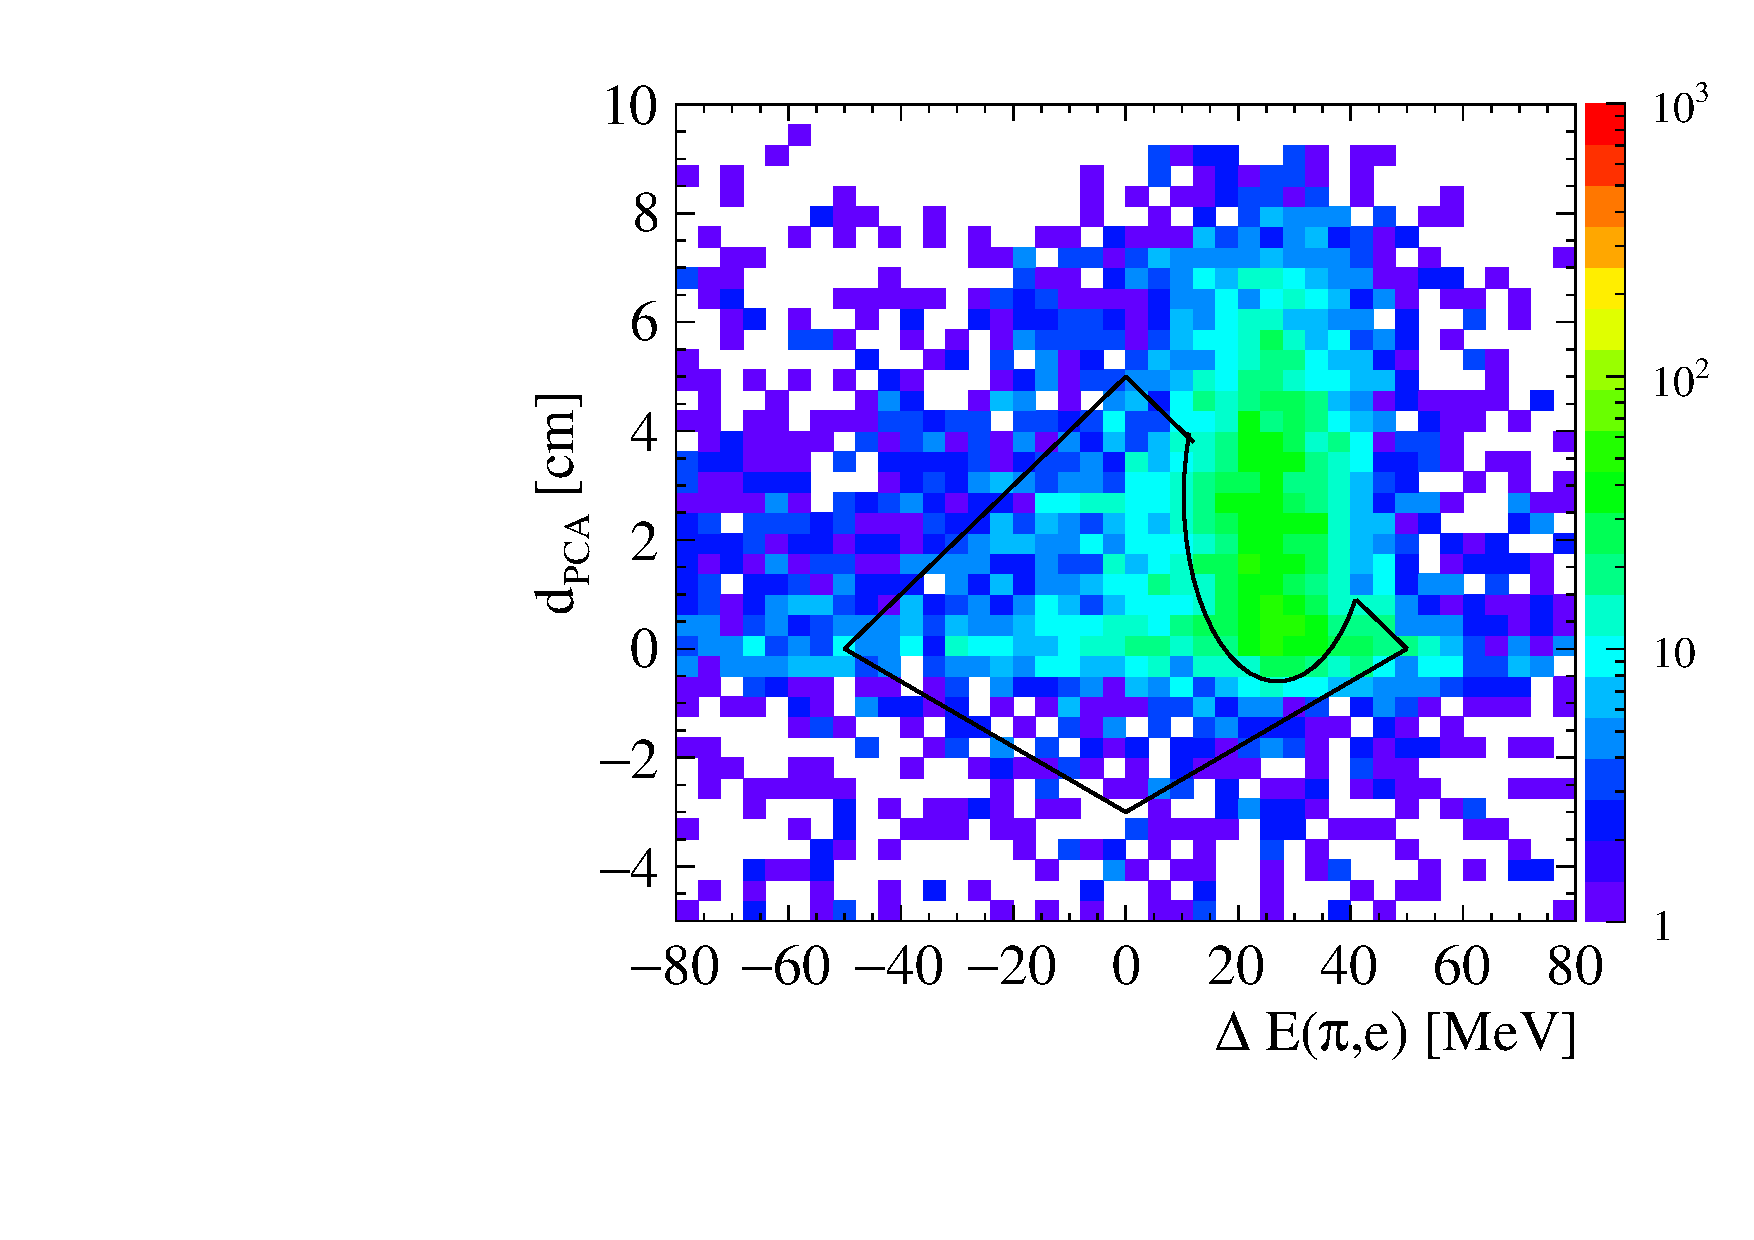
\includegraphics[width=1.0\textwidth]{Chapter7_analysis_kloe/img/dpca_de_background}
    \caption{Background events (MC)}
  \end{subfigure}
  %
  \begin{subfigure}{0.45\textwidth}
    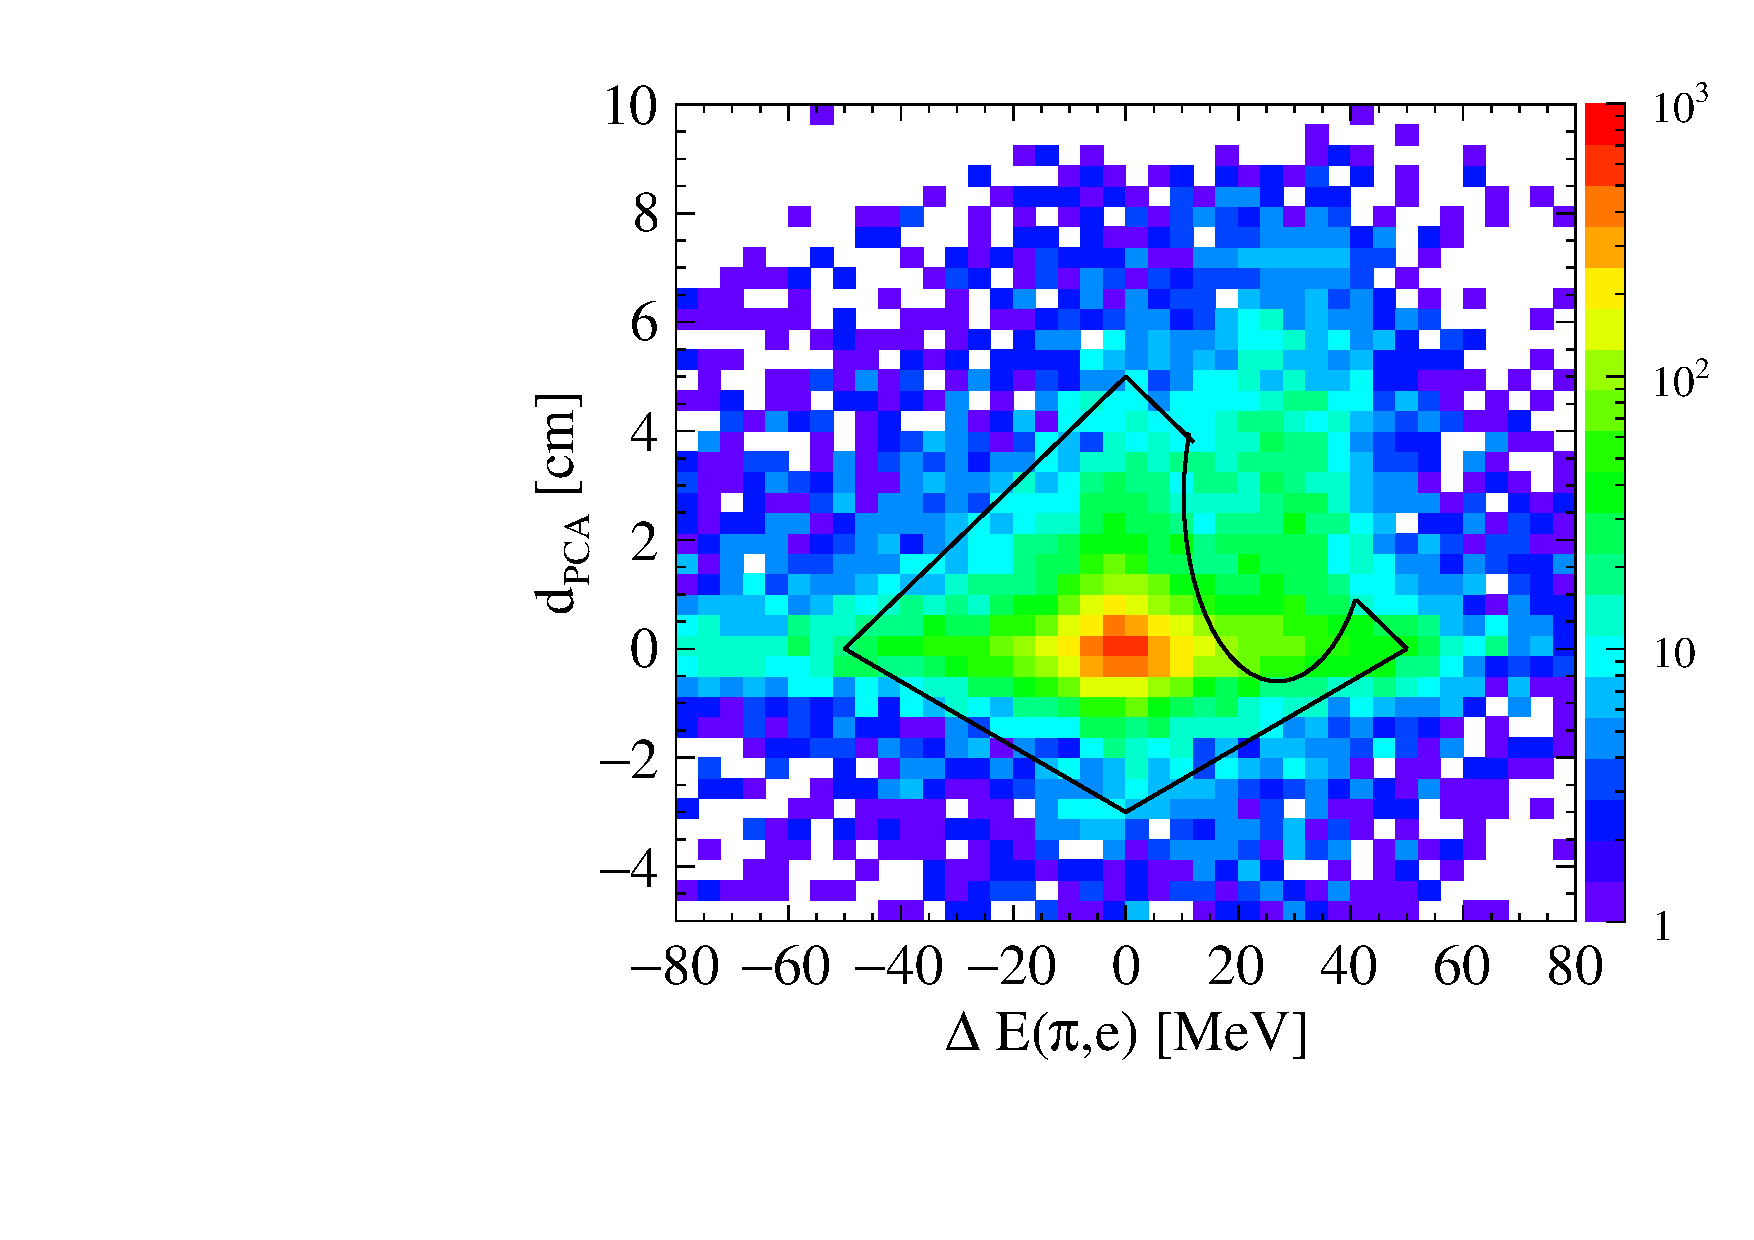
\includegraphics[width=1.0\textwidth]{Chapter7_analysis_kloe/img/dpca_de_data}
    \caption{All data events}
  \end{subfigure}
  \caption{Difference between two tracks' distances of closest approach to the $\phi$ decay point vs\. difference between missing energy and momentum in the kaon decay. Events are accepted if they lie inside the region defined by a rhombus with exclusion of an elliptical region, marked with black solid line.}\label{fig:dpca_de_cut}
\end{figure}

\subsection{Determination of lepton charge and kaon decay times' difference}\label{sec:charge_and_dt}
Determination of the \Ts-asymmetric ratios of double decay rates defined in Equations~\ref{eq:r2def} and~\ref{eq:r4def} requires that the $\Ks\Kl\to\pi e\nu\;3\pi^0$ dataset is split into two subsamples depending on whether the lepton in the $\Ks$ decay was an electron or a positron. This charge identification is based on the curvature of the track identified as corresponding to a particle of electron mass. Sign of the curvature with respect to the known direction of the magnetic field in KLOE is used to determine the sign of the lepton charge in an event.

Moreover, the $R_2^{exp}$ and $R_4^{exp}$ ratios are functions of the difference between proper times of the two kaon decays. Therefore, for each of the studied events, the following difference must be precisely calculated:
\begin{equation}
  \label{eq:dt_definition}
  \Delta t = t'_{3\pi^{0}} - t'_{\pi e \nu},  
\end{equation}
where $t'_{\pi e \nu}$ and $t'_{3\pi^{0}}$ are times of decays identified by respective final states, expressed in the frames of reference of the decaying kaons. In case of the $\pi e\nu$ decay, decay time is obtained from the path travelled by the kaon between the $\phi$ decay point and a common vertex of the two tracks and the velocity calculated from K meson momentum. As transformation to the kaon rest frame is performed along the travelled path, its proper decay time reads:
\begin{eqnarray}
  \label{eq:ks_proper_time}
  t'_{\pi e\nu} &=& \frac{L}{c\beta}\frac{1}{\gamma} = \frac{Lm_{\kaon}}{c|\vec{p}_{\kaon}|},\\
  L &=& |\vec{\mathbf{v}}_{\phi} - \vec{\mathbf{v}}_{\pi e \nu}|,
\end{eqnarray}
where $\vec{\mathbf{v}}_{\phi}$ and $\vec{\mathbf{v}}_{\pi e \nu}$ denote position vectors of the respective vertices.

The time of the other kaon decay into $3\pi^0$ may be estimated in a similar manner using the reconstructed decay vertex position or, alternatively, using the time resulting directly from trilaterative reconstruction (see~\sref{sec:gps_kloe}). However, due to limited accuracy of this reconstruction based on times and positions recorded by the electromagnetic calorimeter (see~\fref{fig:resolutions_nofit}), neither of this methods has a time resolution comparable with the one of $t_{\pi e \nu}$ which is at the level of 1~$\tau_S$. As the estimation of proper $\Kl\to 3\pi^{0}$ decay time analogical to~\eref{eq:ks_proper_time} depends on both the decay vertex location (through travelled path $L_{\Kl}$) and kaon momentum, its resolution can be improved by means of a kinematic fit imposing additional constraints binding $L_{K_L}$ and $\vec{p}_{\Kl}$ as described in~\sref{sec:kinfit}.


\subsection{Rejection of background from $\Ks\to\pi^0\pi^0$}\label{sec:ks2pi0_rejection}
After the selection discussed up to this point, as tested with KLOE MC simulations, about \SI{12}{\percent} of the chosen events are constituted by the $\Ks\to\pi^0\pi^0$ and $\Kl\to\pi e\nu$ processes where the $\Ks$ decay along with additional EMC clusters originating from cluster splitting or machine background was misidentified as an early $\Kl\to 3\pi^0$ decay. Such cases are characterized by a small difference between both kaon decay times as otherwise the semileptonic decay vertex would not be recorded in the fiducial volume around the $\phi$~decay point. To remove this background component, EMC clusters coming from prompt photons (i.e.\ photons which originate close to the primary interaction vertex) are identified by testing the value of $R/(cT_{clu})$~\cite{kloe_memo_146}, where $R$ is the distance between average $\phi$~decay location and position of an EMC cluster, $T_{clu}$ is the cluster recording time and $c$ is the velocity of light. This ratio is close to unity for prompt photons from $\Ks\to\pi^0\pi^0$ which differentiates them from those created in $\Kl$ decay occurring further in the detector volume as shown in~\fref{fig:rtc} (left).

\begin{figure}[h!]
  \centering
  \begin{tikzpicture}
    \node[anchor=south west,inner sep=0] at (0,0) 
    {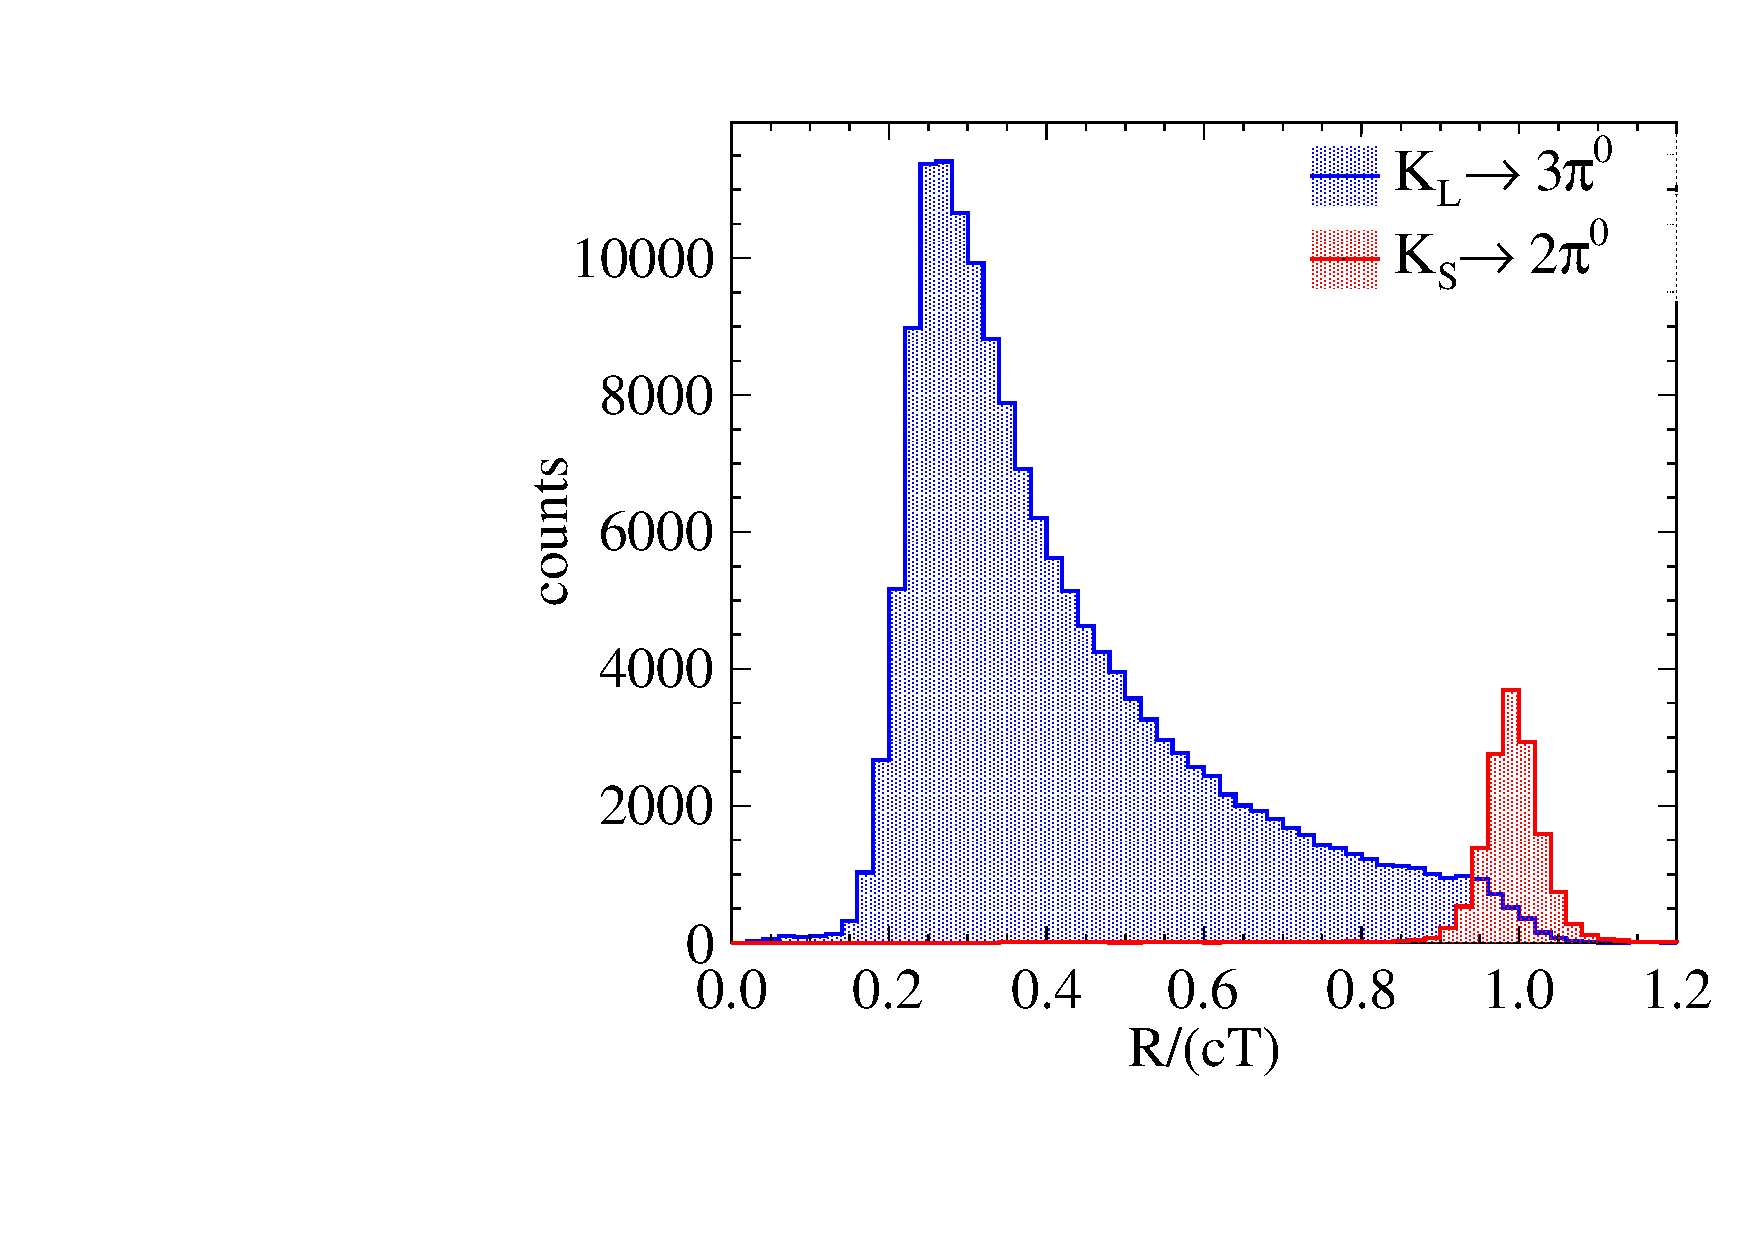
\includegraphics[width=0.45\textwidth]{Chapter7_analysis_kloe/img/rtc}};
    \draw[black, thick, dashed] (5.22,0.8) -- (5.22,4.0);
  \end{tikzpicture}
  \hspace{1em}
    \begin{tikzpicture}
    \node[anchor=south west,inner sep=0] at (0,0) 
    {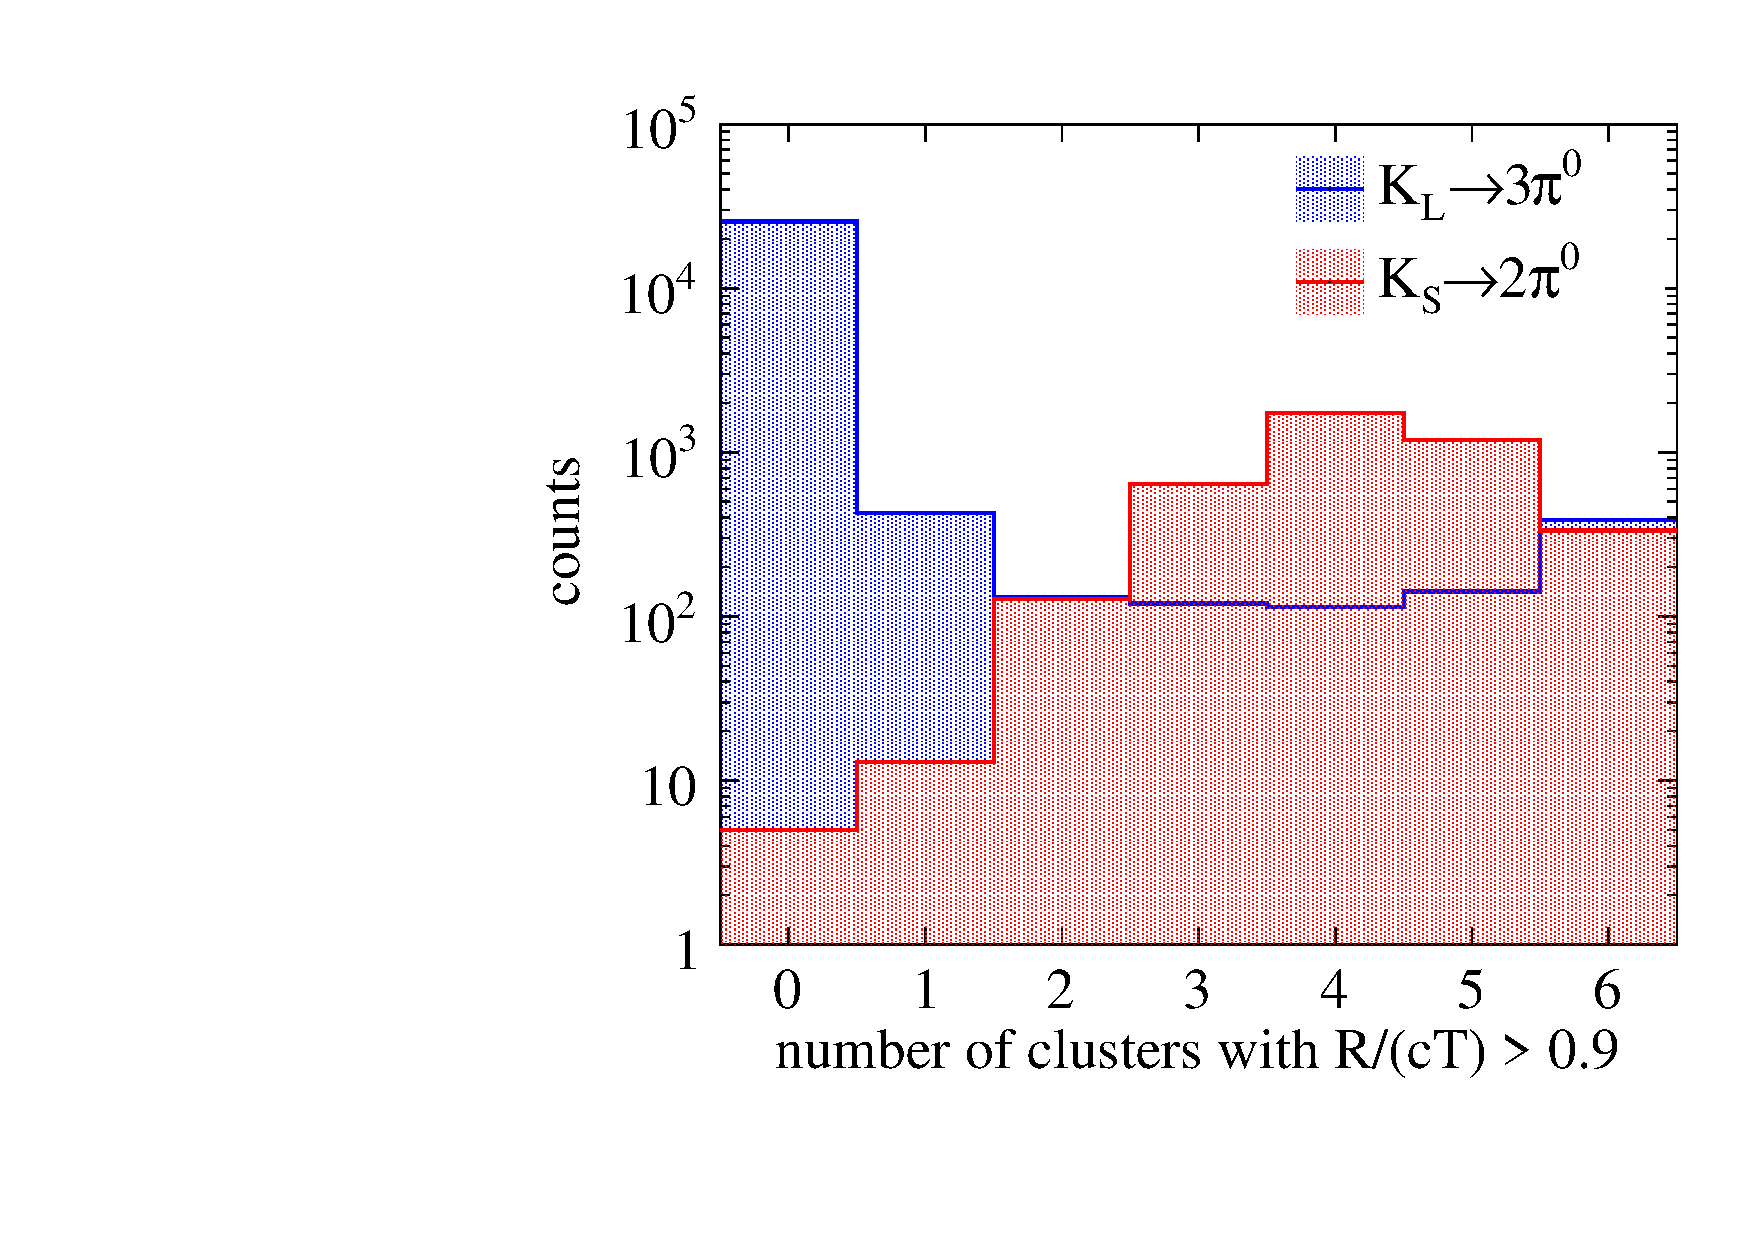
\includegraphics[width=0.45\textwidth]{Chapter7_analysis_kloe/img/n_rtc}};
    \draw[black, thick, dashed] (2.65,0.8) -- (2.65,5.46);
  \end{tikzpicture}  
  \caption{Left: Ratio of distance travelled by a hypothetical prompt photon from the primary interaction vertex to an EMC cluster to the product of cluster recording time and velocity of light. Distributions are presented for MC-simulated events of $\Ks\to\pi^0\pi^0$ and $\Kl\to 3\pi^0$. Right: multiplicity of clusters with $R/(cT_{clu})$ larger than 0.9 (see the dashed line in the left panel). Dashed vertical lines denote selection cuts used in the analysis.}\label{fig:rtc} 
\end{figure}

In order to detect the $\Ks\to\pi^0\pi^0$ events, clusters from prompt photons for which $R/(cT_{clu})>0.9$ (compare~\fref{fig:rtc} (left)) were counted in each event. The resulting prompt photon multiplicities checked with MC simulations for $\Ks\to\pi^0\pi^0$ and $\Kl\to 3\pi^0$ decays are presented in the right panel of~\fref{fig:rtc}. Strong discrimination of the $\pi^0\pi^0$ background is obtained by rejecting events which contain two or more clusters for which $R/(cT_{clu})>0.9$.
%
% TODO: odnosnik do sekcji z wydajnosciami i do sekcji gdzie dyskutuje sie uzyty zakres delta t
%
The cost of this requirement is a significant reduction of efficiency for the $\Kl\to 3\pi^0$ signal events with an early $\Kl$ decay, corresponding to time differences between both kaon decays in the range (0;12)~$\tau_S$. This region, however, is not crucial for the \Ts~symmetry test considered in this work.

\subsection[Rejection of background from $\Ks\to\pi^+\pi^-(\to\pi\mu\nu)$\newline and \mbox{$\Ks\to\pi^+\pi^-(\gamma)$} decays]{Rejection of background from $\Ks\to\pi^+\pi^-(\to\pi\mu\nu)$ and \mbox{$\Ks\to\pi^+\pi^-(\gamma)$} decays}\label{sec:pimu_rejection}
%
% Zaktualizować S/B
%
Although the cuts presented in the previous section significantly improve signal to background ratio in the selected event sample (from about 2.7 to about 11.3), almost \SI{10}{\percent} of the selected events was still constituted by the $\Ks\to\pi^+\pi^-(\gamma)$ and $\Ks\to\pi^+\pi^-\to\pi\mu\nu$ decays. The remaining background is especially problematic due to its presence over a large range of time differences between kaons' decays and strong charge asymmetry visible in the two MC-based distributions in~\fref{fig:csps-dt-before}, plotted separately for events with negative and positive charge of the particle identified as lepton in the $\Ks\to\pi e\nu$ decay.
\begin{figure}[h!]
  \captionsetup[subfigure]{justification=centering}
  \centering
  \begin{subfigure}{0.45\textwidth}
  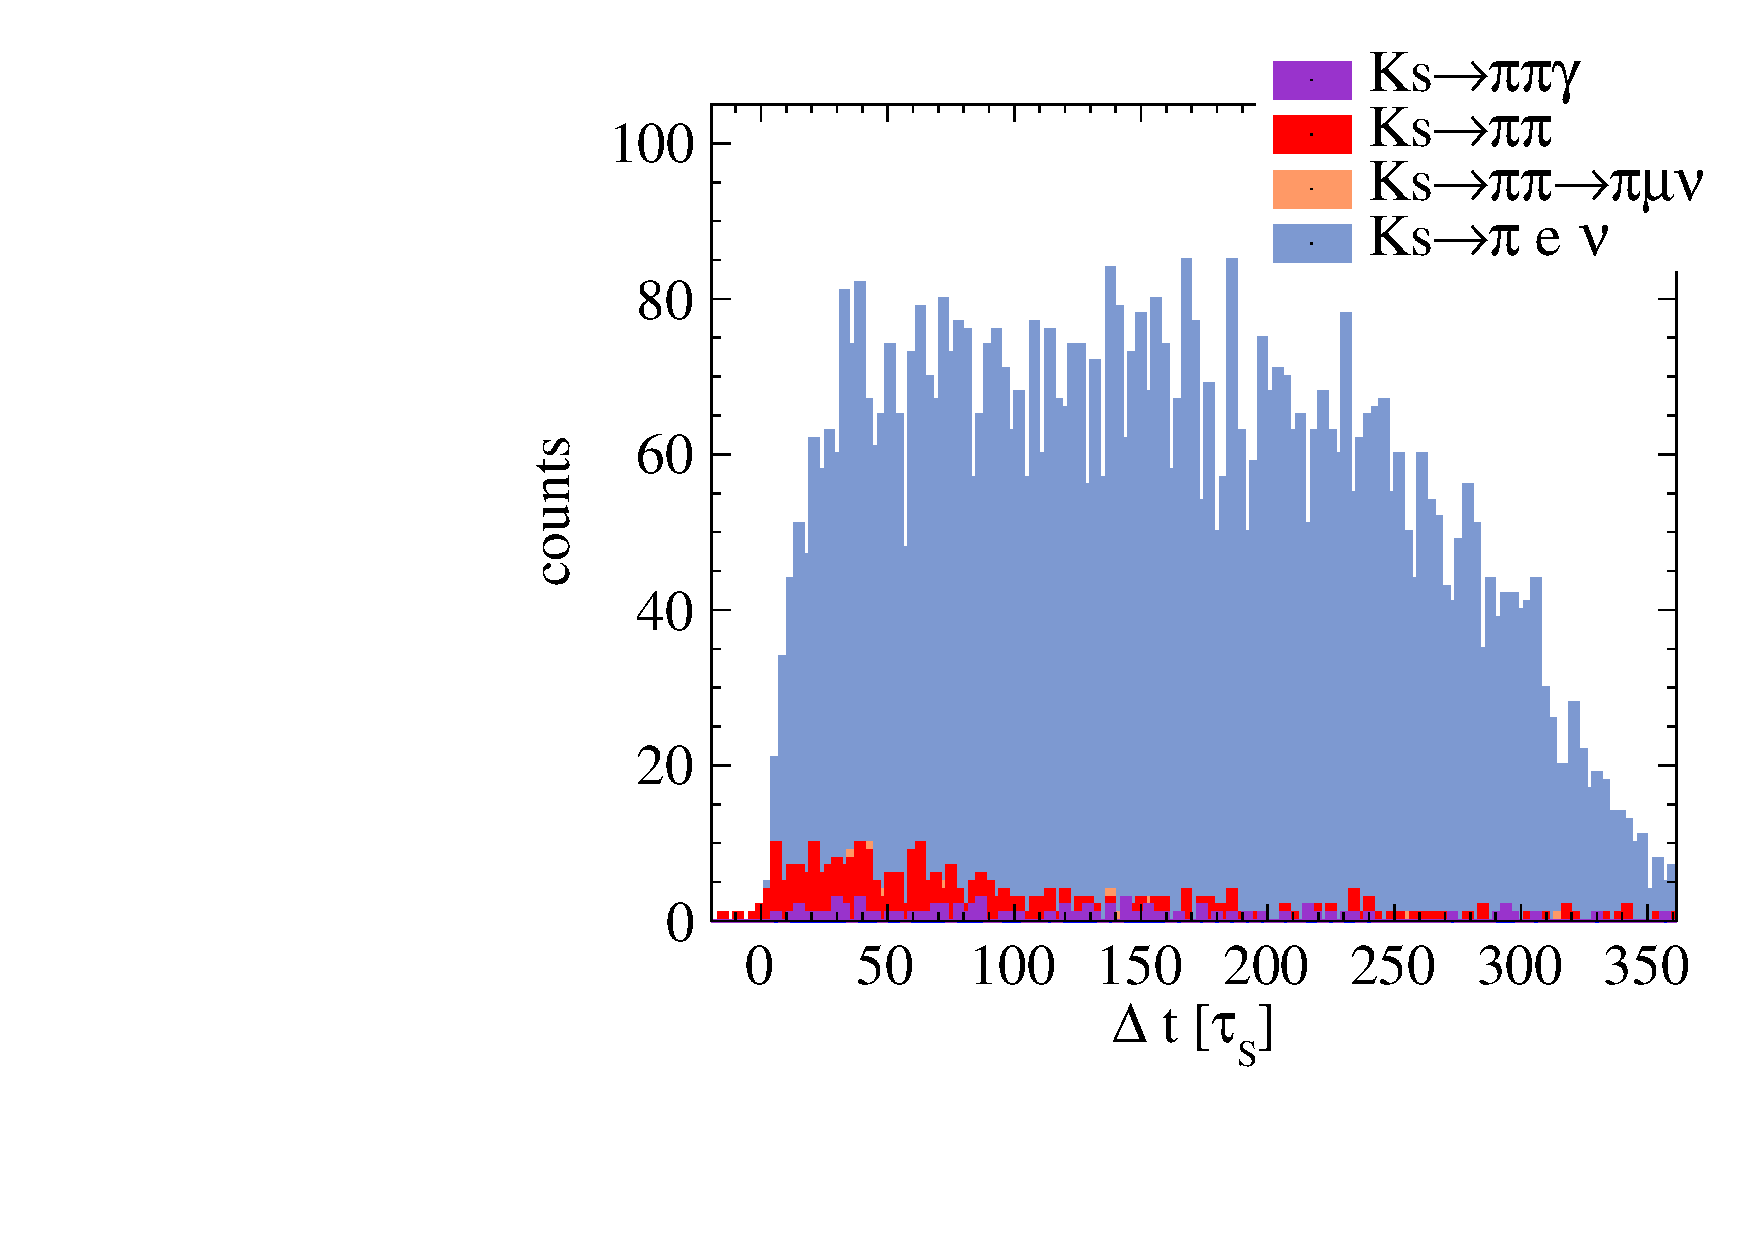
\includegraphics[width=1.0\textwidth]{Chapter7_analysis_kloe/img/csps/with_bcg_eminus}
  \caption{Events with a track identified as electron.}
  \end{subfigure}
  % 
  \begin{subfigure}{0.45\textwidth}
  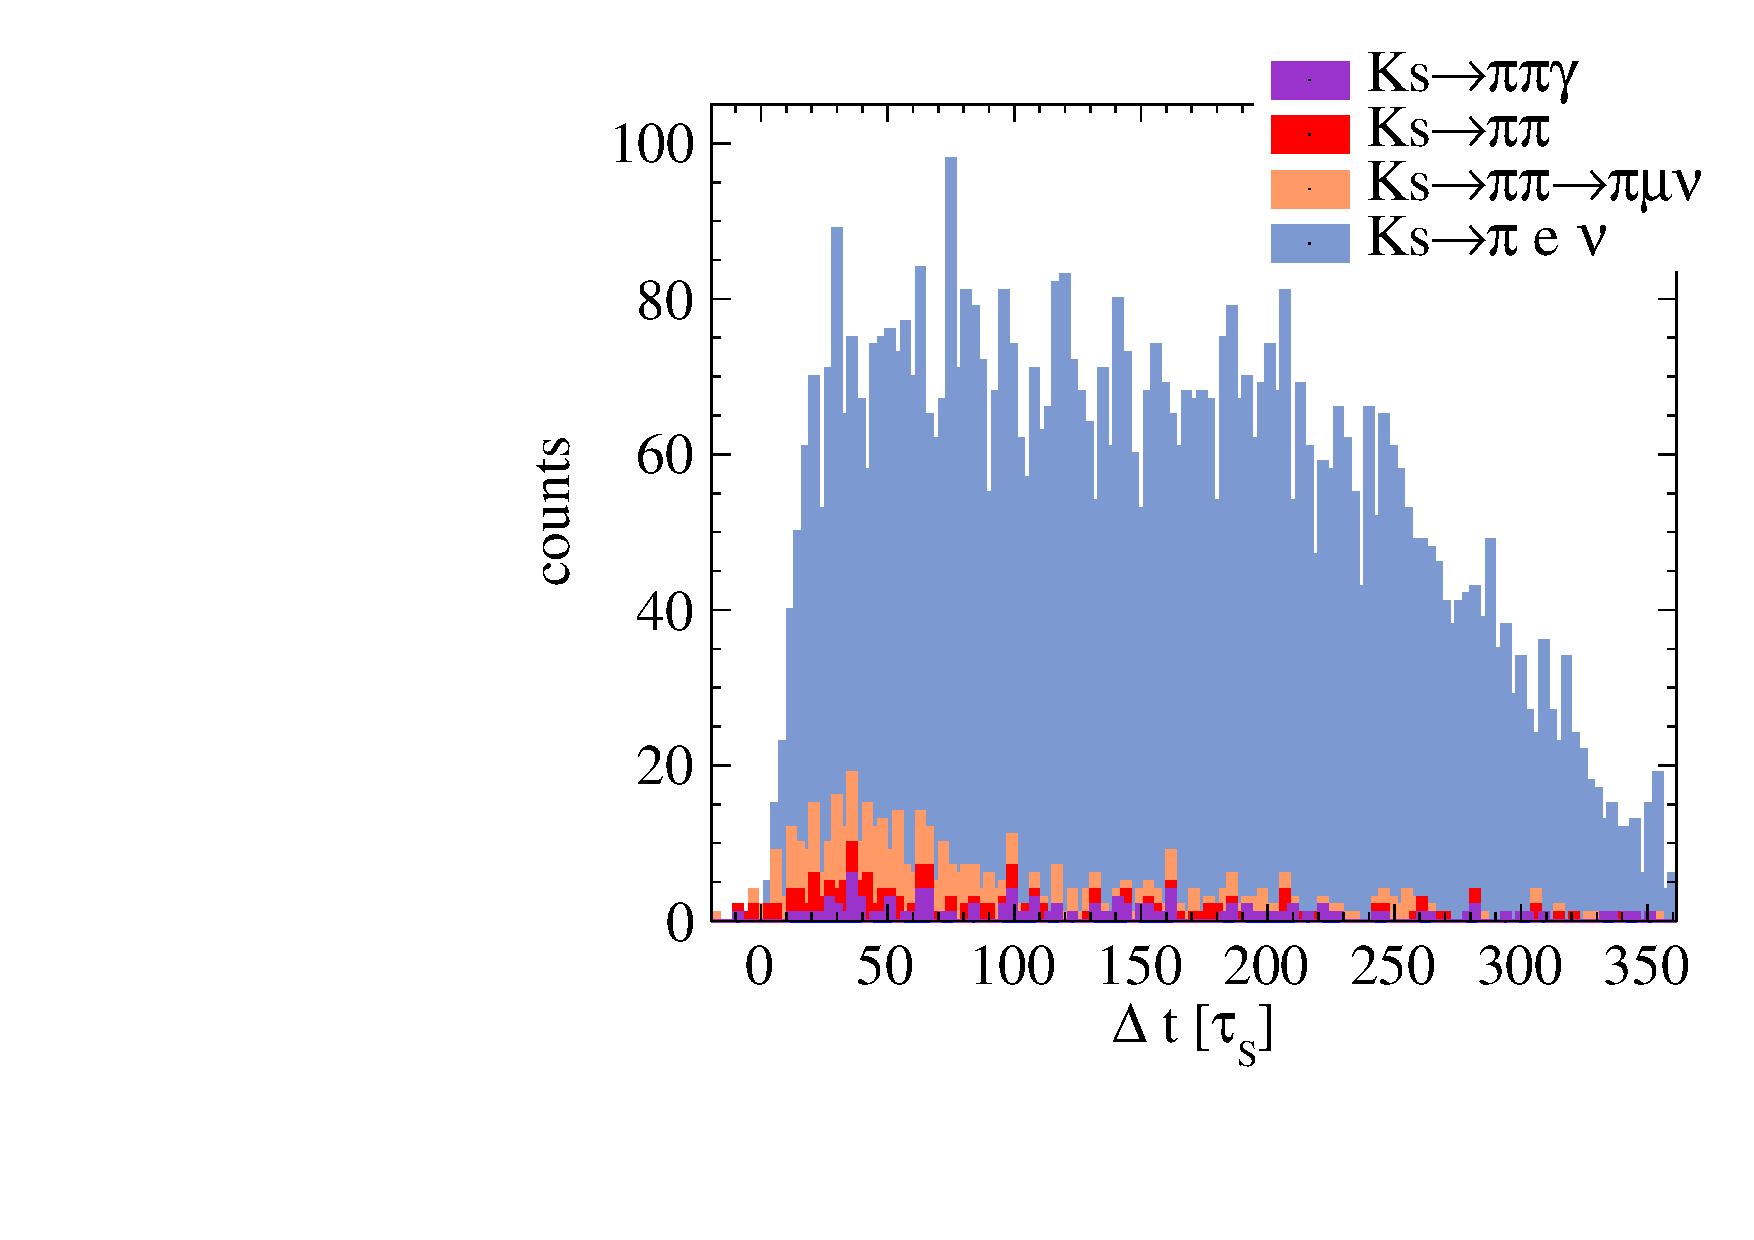
\includegraphics[width=1.0\textwidth]{Chapter7_analysis_kloe/img/csps/with_bcg_eplus}
  \caption{Events with a track identified as positron.}
  \end{subfigure}
  \caption{Stacked MC-based distributions of kaons' decay time difference for signal and background events surviving the selection up to (inclusive) the cut on $d_{PCA}$ and $\Delta E(\pi,e)$.}\label{fig:csps-dt-before}
\end{figure}

In order to reduce the remaining background components, a set of classifiers based on the properties of tracks and clusters was prepared to distinguish electrons and positrons from pion and muons. Classification relied primarily on the fact that electromagnetic showers created in the KLOE calorimeter by interactions of electrons are considerably different than in case of charged pions and muons. While the former tend to release a large amount of energy at their first interaction in the calorimeter, muons and charged pions deposit energy rather uniformly along their path travelled through the material, with a possible greater deposit at a large depth due to the Bragg peak~\cite{graziani_anns}. To probe the structure of such electromagnetic showers, the EMC segmentation into layers was used (see~\sref{sec:emc}). As every calorimeter module in KLOE is composed of five layers located at increasing depths, energies deposited by a given particle in particular layers as well as the total number of layers with a non-zero deposited energy provide information specific to the type of interacting particle. Additionally, the total deposited energy of the whole EMC cluster and the particle momentum estimated using the associated DC track were also used for classification. 

Two classifiers were constructed using a neural network implementation from the Toolkit for Multivariate Analysis~\cite{Hocker:2007ht}. Each classifier acted on an ensemble constituted by a DC track and its associated EMC cluster and attempted to distinguish those originating from an electron/positron and from a pion ($e/\pi$ classifier) or a muon ($e/\mu$ classifier). Multilayer perceptrons (MLPs) with five inputs and one output were employed as classifiers. Details of input variables and implemented classifiers are presented in~\aref{appendix:clasifiers}.

\begin{figure}[h!]
  \centering
  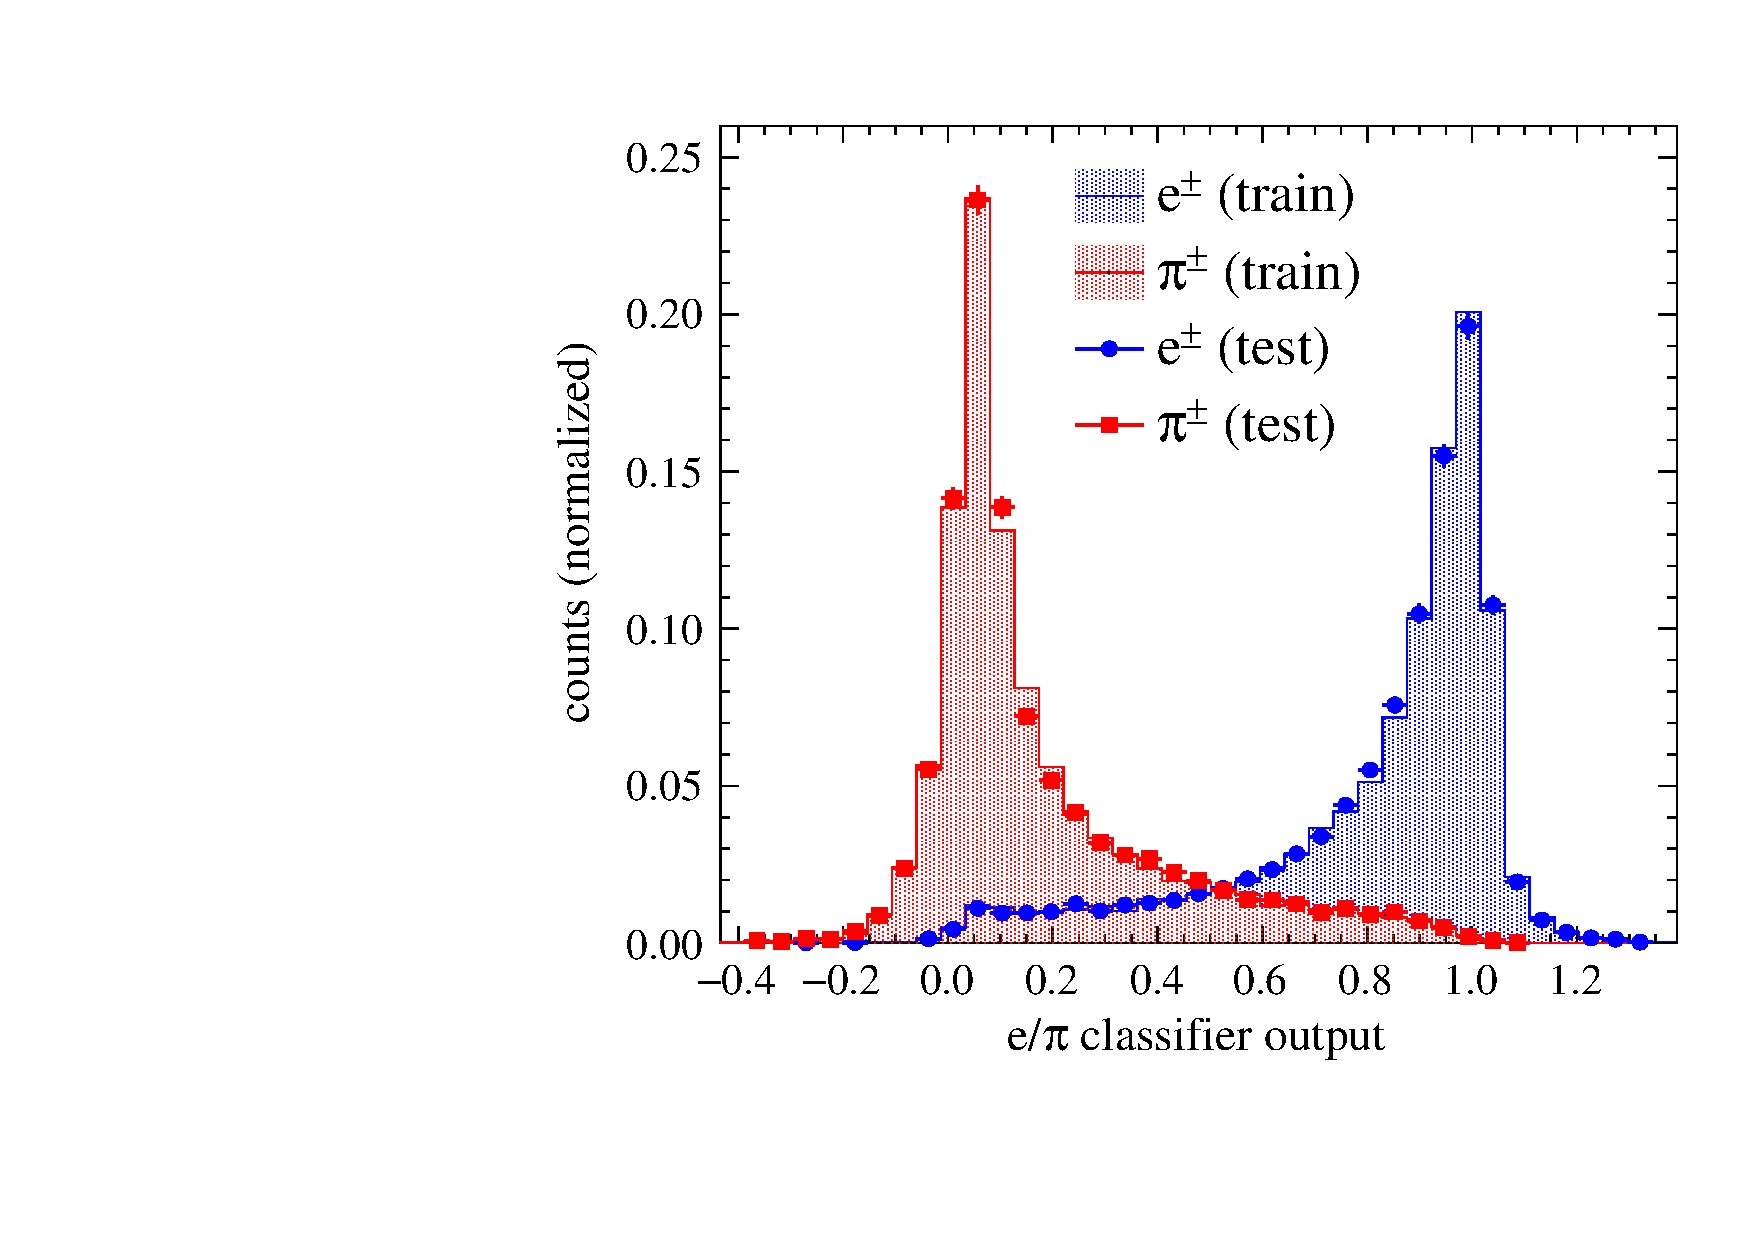
\includegraphics[width=0.45\textwidth]{Chapter7_analysis_kloe/img/csps/epi_output}
  \hspace{1em}  
  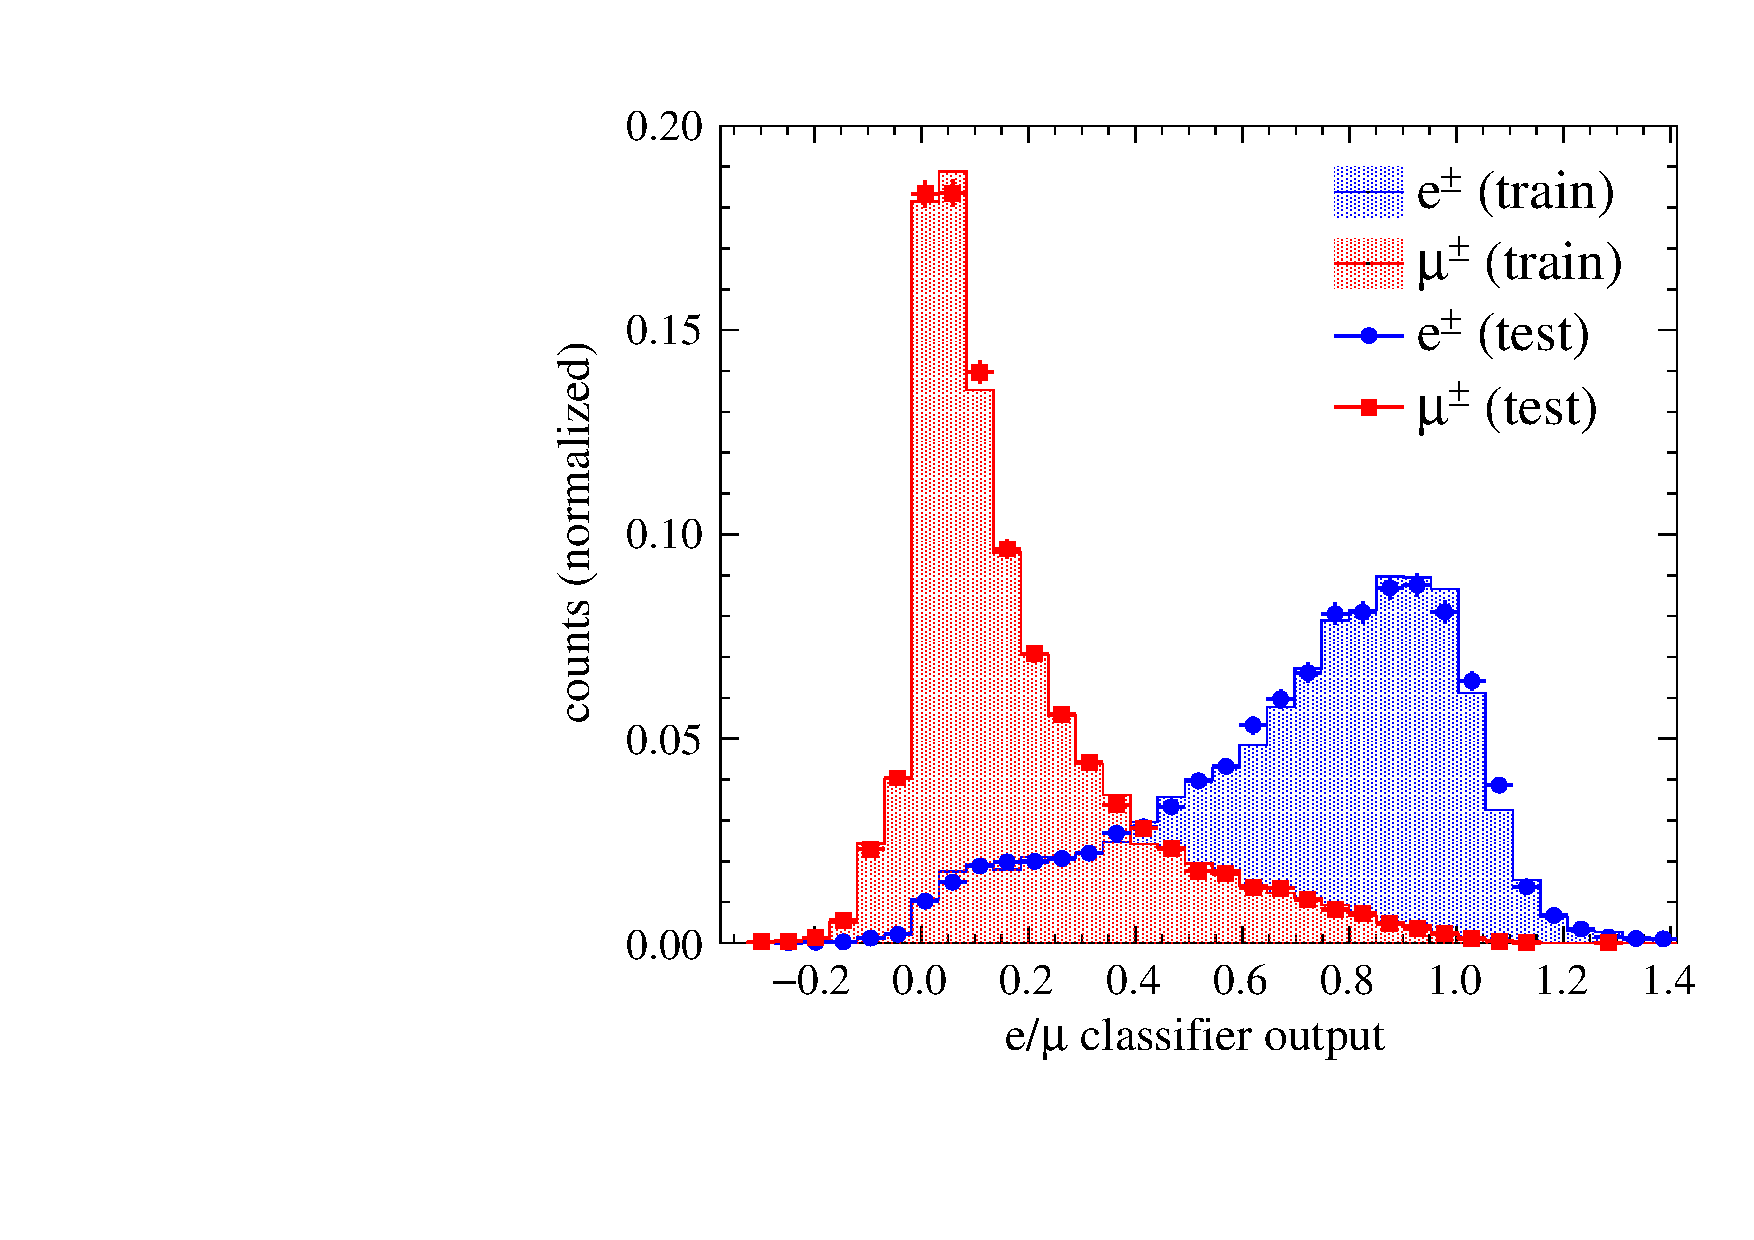
\includegraphics[width=0.45\textwidth]{Chapter7_analysis_kloe/img/csps/emu_output}
  \caption{Output values of artificial neural networks used as electron/pion classifier (left) and as electron/muon classifier (right), obtained with test and training data samples. }\label{fig:mlp_outputs}
\end{figure}

In order to avoid adjusting of the MLPs to artifacts specific to MC simulations, the classifiers were trained solely using data. As the properties of track and clusters under study do not depend on the origin of the particles, semileptonic decays of the long-lived neutral kaon were used to obtain training and test samples of electron/positron, muon and charged pion tracks. To this end, the event selection of $\Ks\Kl\to\pi^+\pi^-\;\pi e\nu$ described in~\sref{sec:t-analysis-2} was used directly to obtain a $\Kl\to\pi e \nu$ sample with a purity at the level of \SI{99}{\percent}. Subsequently, the selection cuts were adjusted to select semileptonic $\Kl$ decays with a muon, yielding the second training sample with a similar purity. Output values of the MLPs used for both classifiers, obtained with test and training samples, are shown in~\fref{fig:mlp_outputs}. The agreement between distributions resulting from training and test data shows that no MLP overtraining effects are present. Although the background discrimination power of the two classifiers, compared in~\fref{fig:mlp_rocs}, is slightly worse in case of electron/muon, both allow for rejection of a large part of the background related to pion and muon tracks while preserving more than \SI{90}{\percent} of signal events with electron/pion tracks.
\begin{figure}[h!]
  \centering
  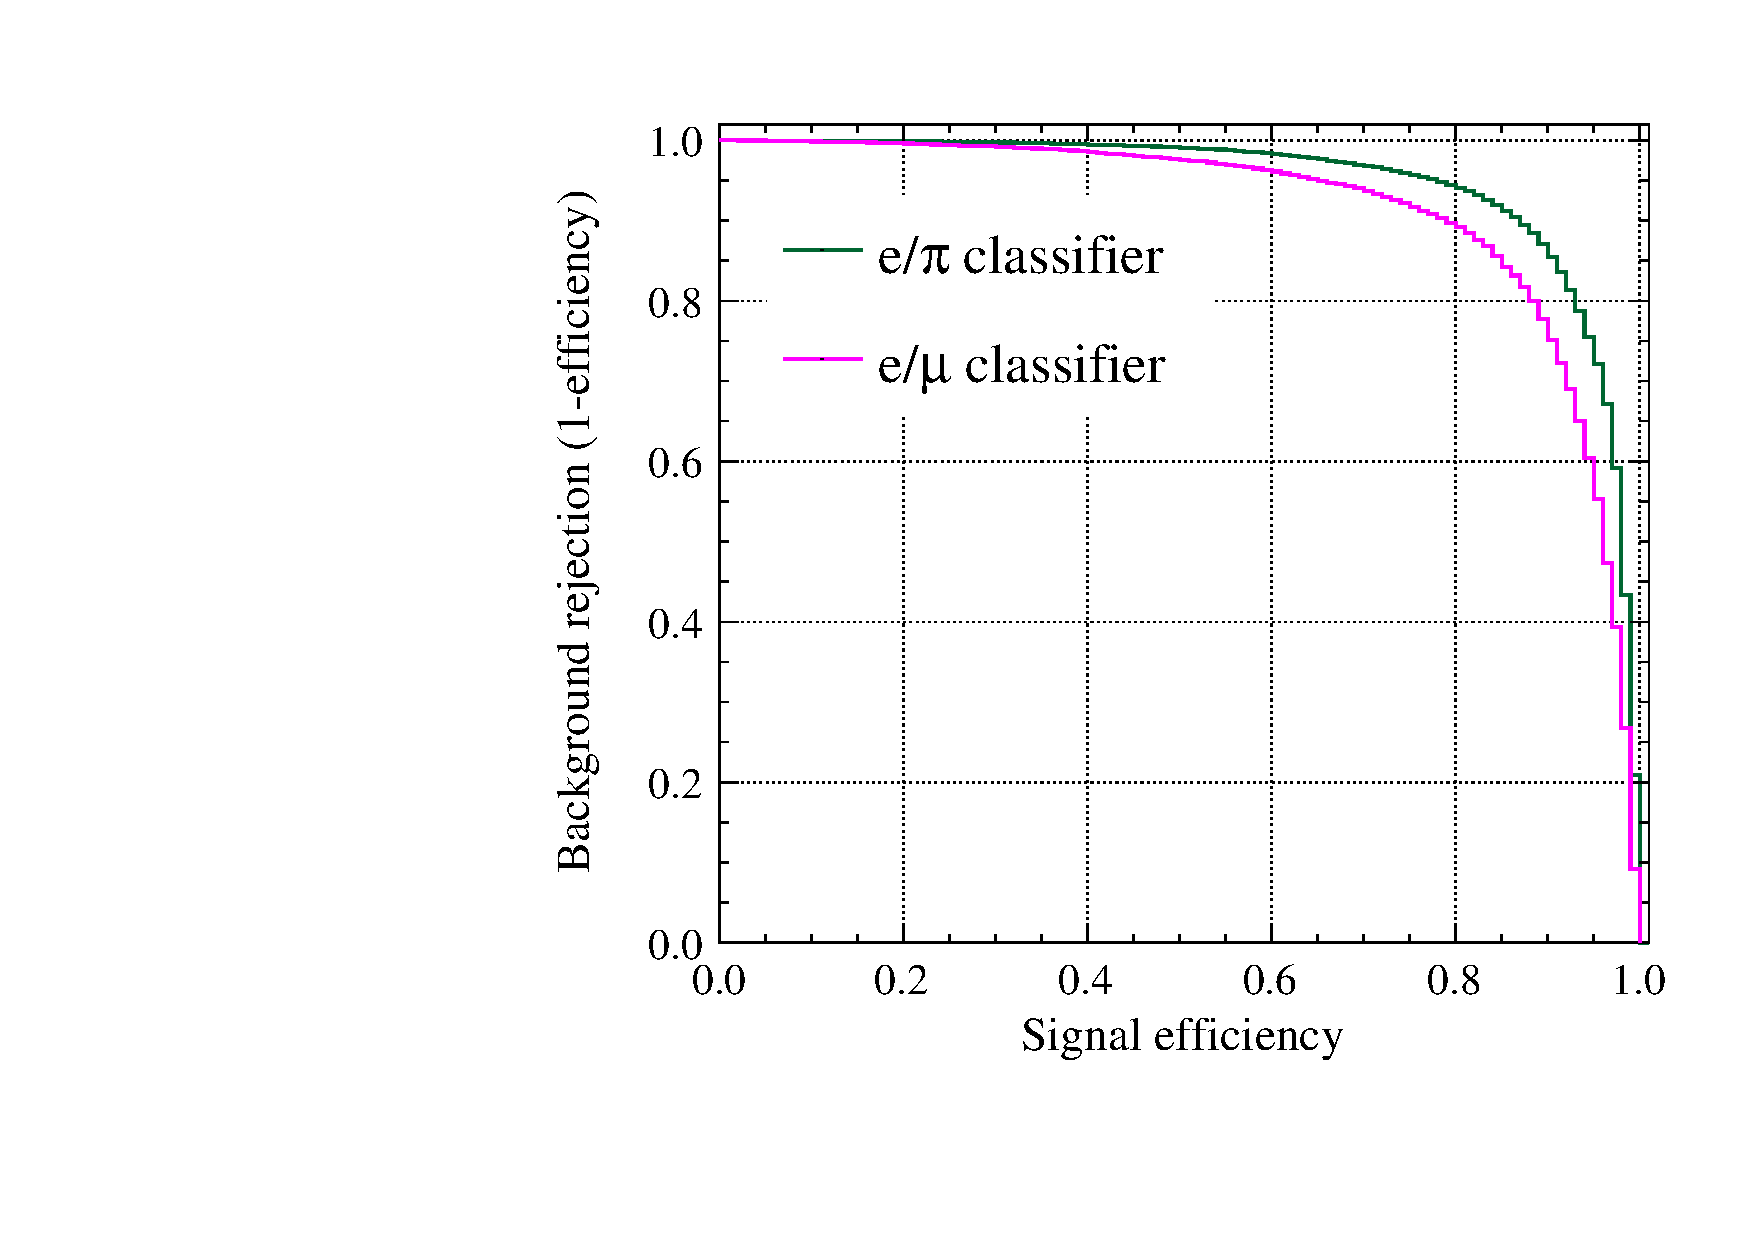
\includegraphics[width=0.45\textwidth]{Chapter7_analysis_kloe/img/csps/rocs}
  \caption{Comparison of background discrimination power and signal efficiency for the $e/\pi$ and $e/\mu$ classifiers.}\label{fig:mlp_rocs}
 \end{figure}

 Discrimination of background was performed by subsequent application of the $e/\pi$ and $e/\mu$ classifiers to the ensemble constituted by DC track identified as electron or positron in the previous analysis steps and its associated EMC cluster. A two-dimensional distribution of both classifier output values displayed in~\fref{fig:mlp_2d} reveals good separation of signal and background events. Events are chosen for the final $\Ks\Kl\to\pi e\nu\;3\pi^0$ sample if they satisfy the following constraint on the sum of both classifiers' outputs:
 \begin{equation*}
   \text{MVA}(e,\pi) + \text{MVA}(e,\mu) > 0.5,
 \end{equation*}
corresponding to an anti-diagonal cut marked in~\fref{fig:mlp_2d}.
 
\begin{figure}[h!]
  \centering
\captionsetup[subfigure]{justification=centering}
  \begin{subfigure}{0.45\textwidth}
    \begin{tikzpicture}
      \node[anchor=south west,inner sep=0] at (0,0) 
      {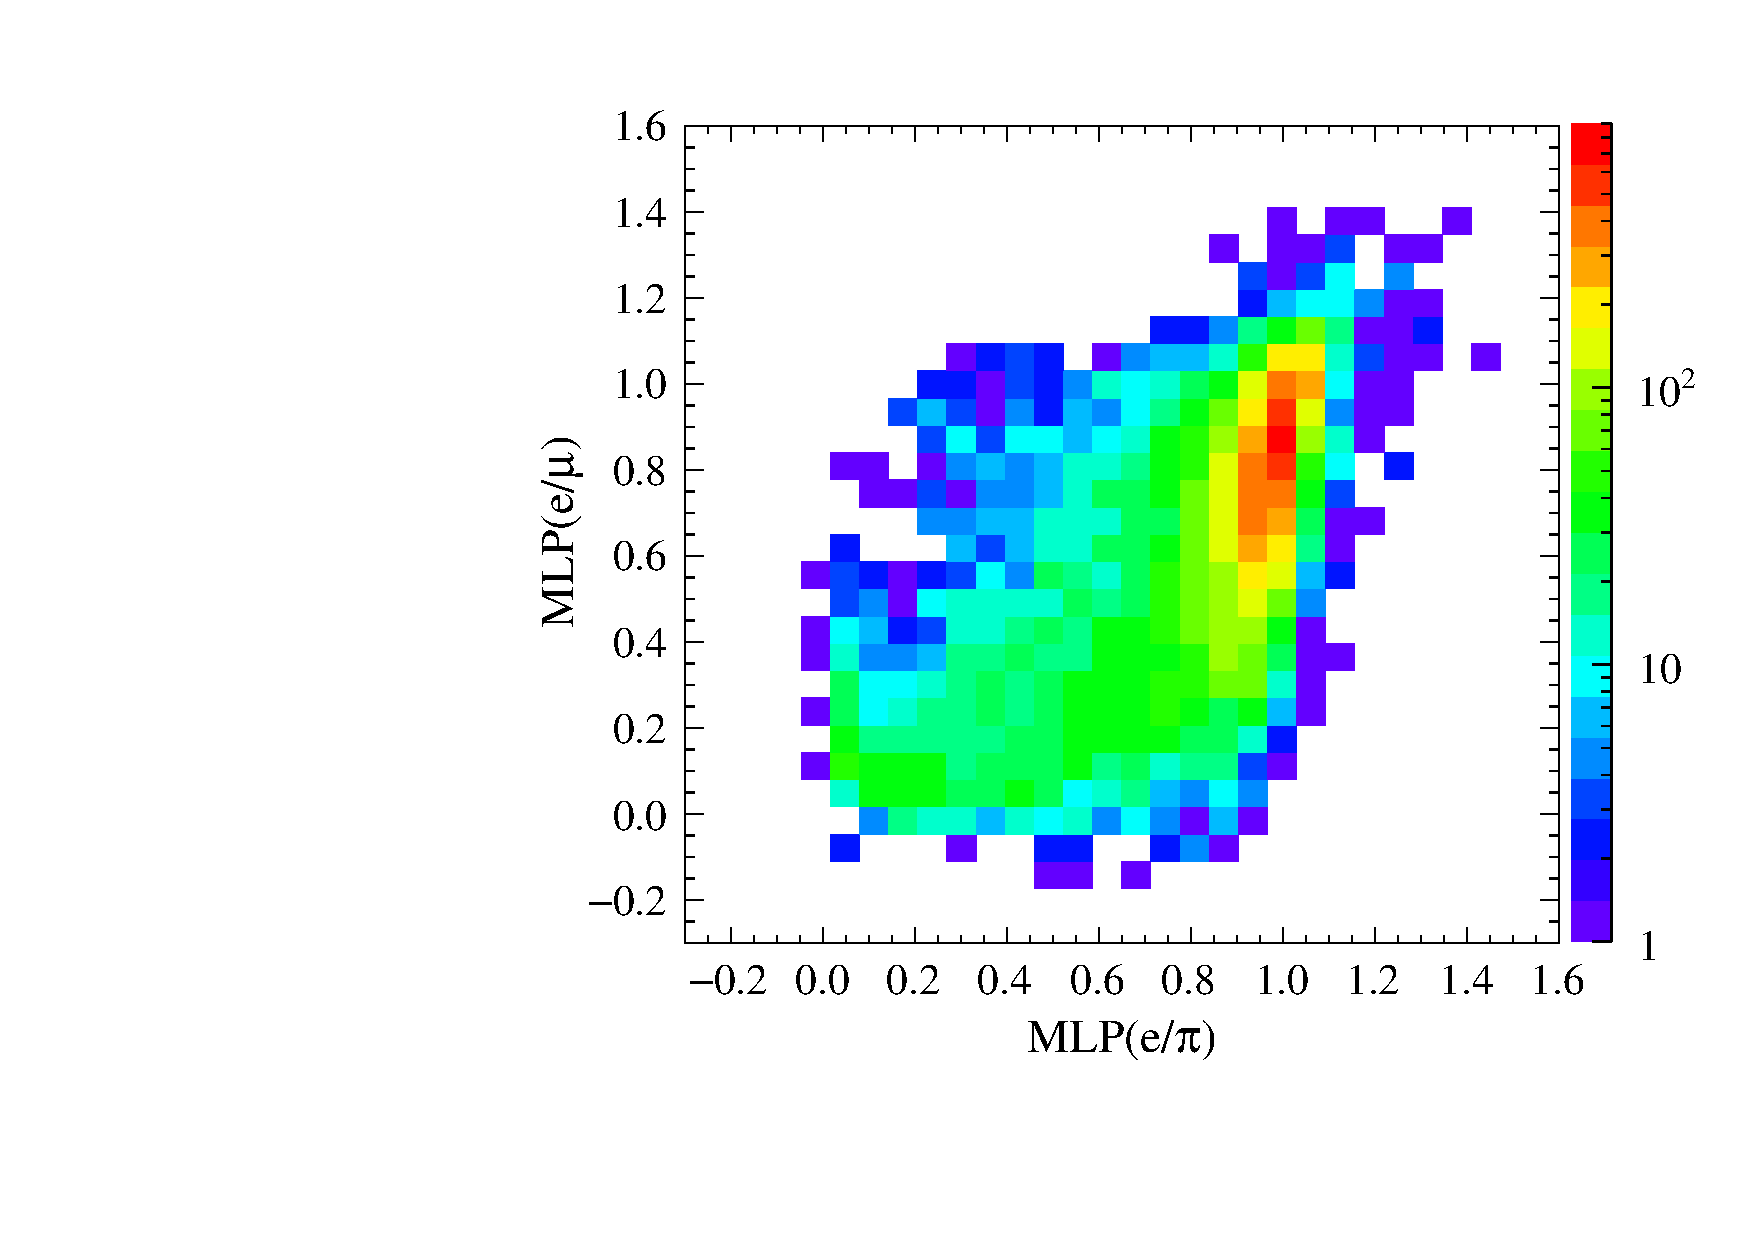
\includegraphics[width=1.0\textwidth]{Chapter7_analysis_kloe/img/csps/emu_vs_epi_signal}};
      \draw[black, thick, dashed] (3.5,1.0) -- (1.0,3.5);
    \end{tikzpicture}  
    \caption{Signal events (MC)}
  \end{subfigure}
  %
  \begin{subfigure}{0.45\textwidth}
    \begin{tikzpicture}
      \node[anchor=south west,inner sep=0] at (0,0) 
      {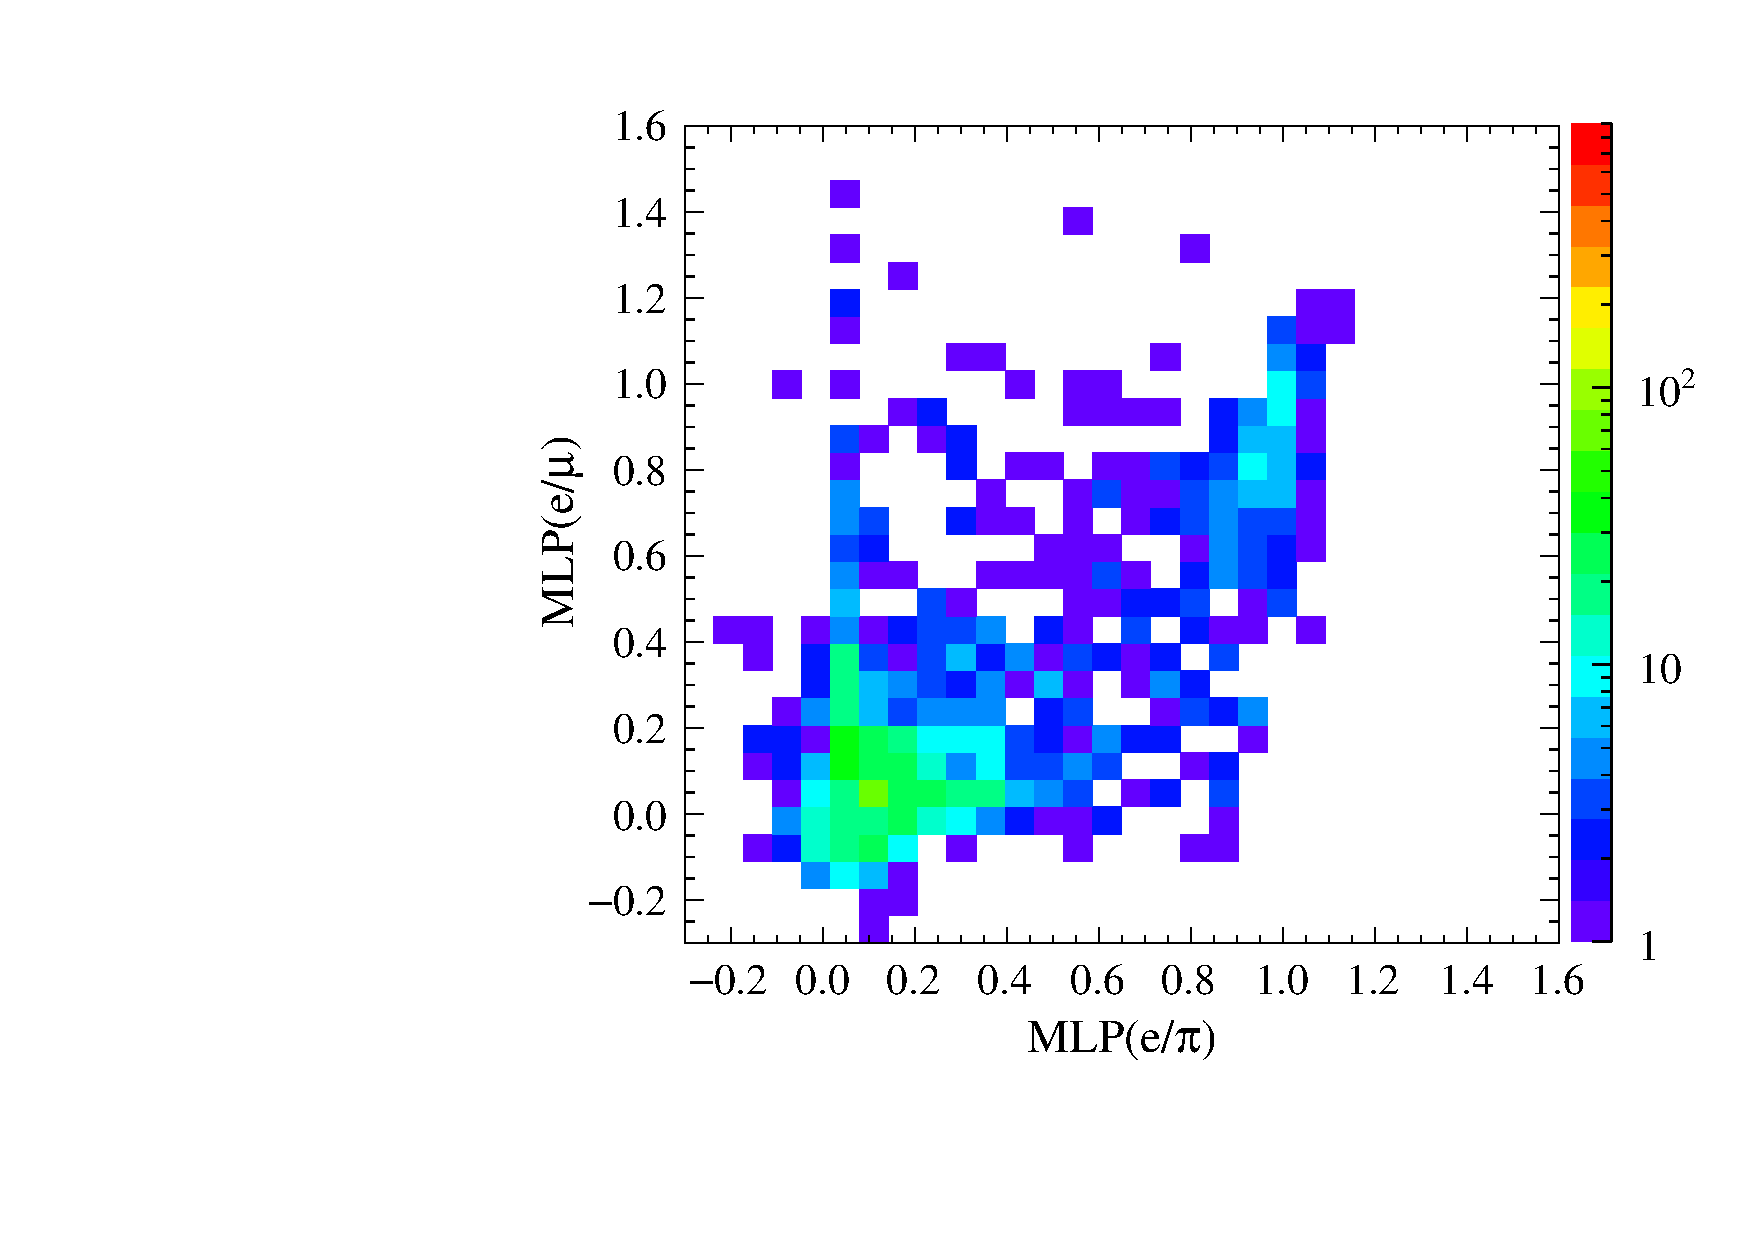
\includegraphics[width=1.0\textwidth]{Chapter7_analysis_kloe/img/csps/emu_vs_epi_background}};
      \draw[black, thick, dashed] (3.5,1.0) -- (1.0,3.5);
    \end{tikzpicture}  
    \caption{Background events (MC)}
  \end{subfigure}
  %
  \begin{subfigure}{0.45\textwidth}
    \begin{tikzpicture}
      \node[anchor=south west,inner sep=0] at (0,0) 
      {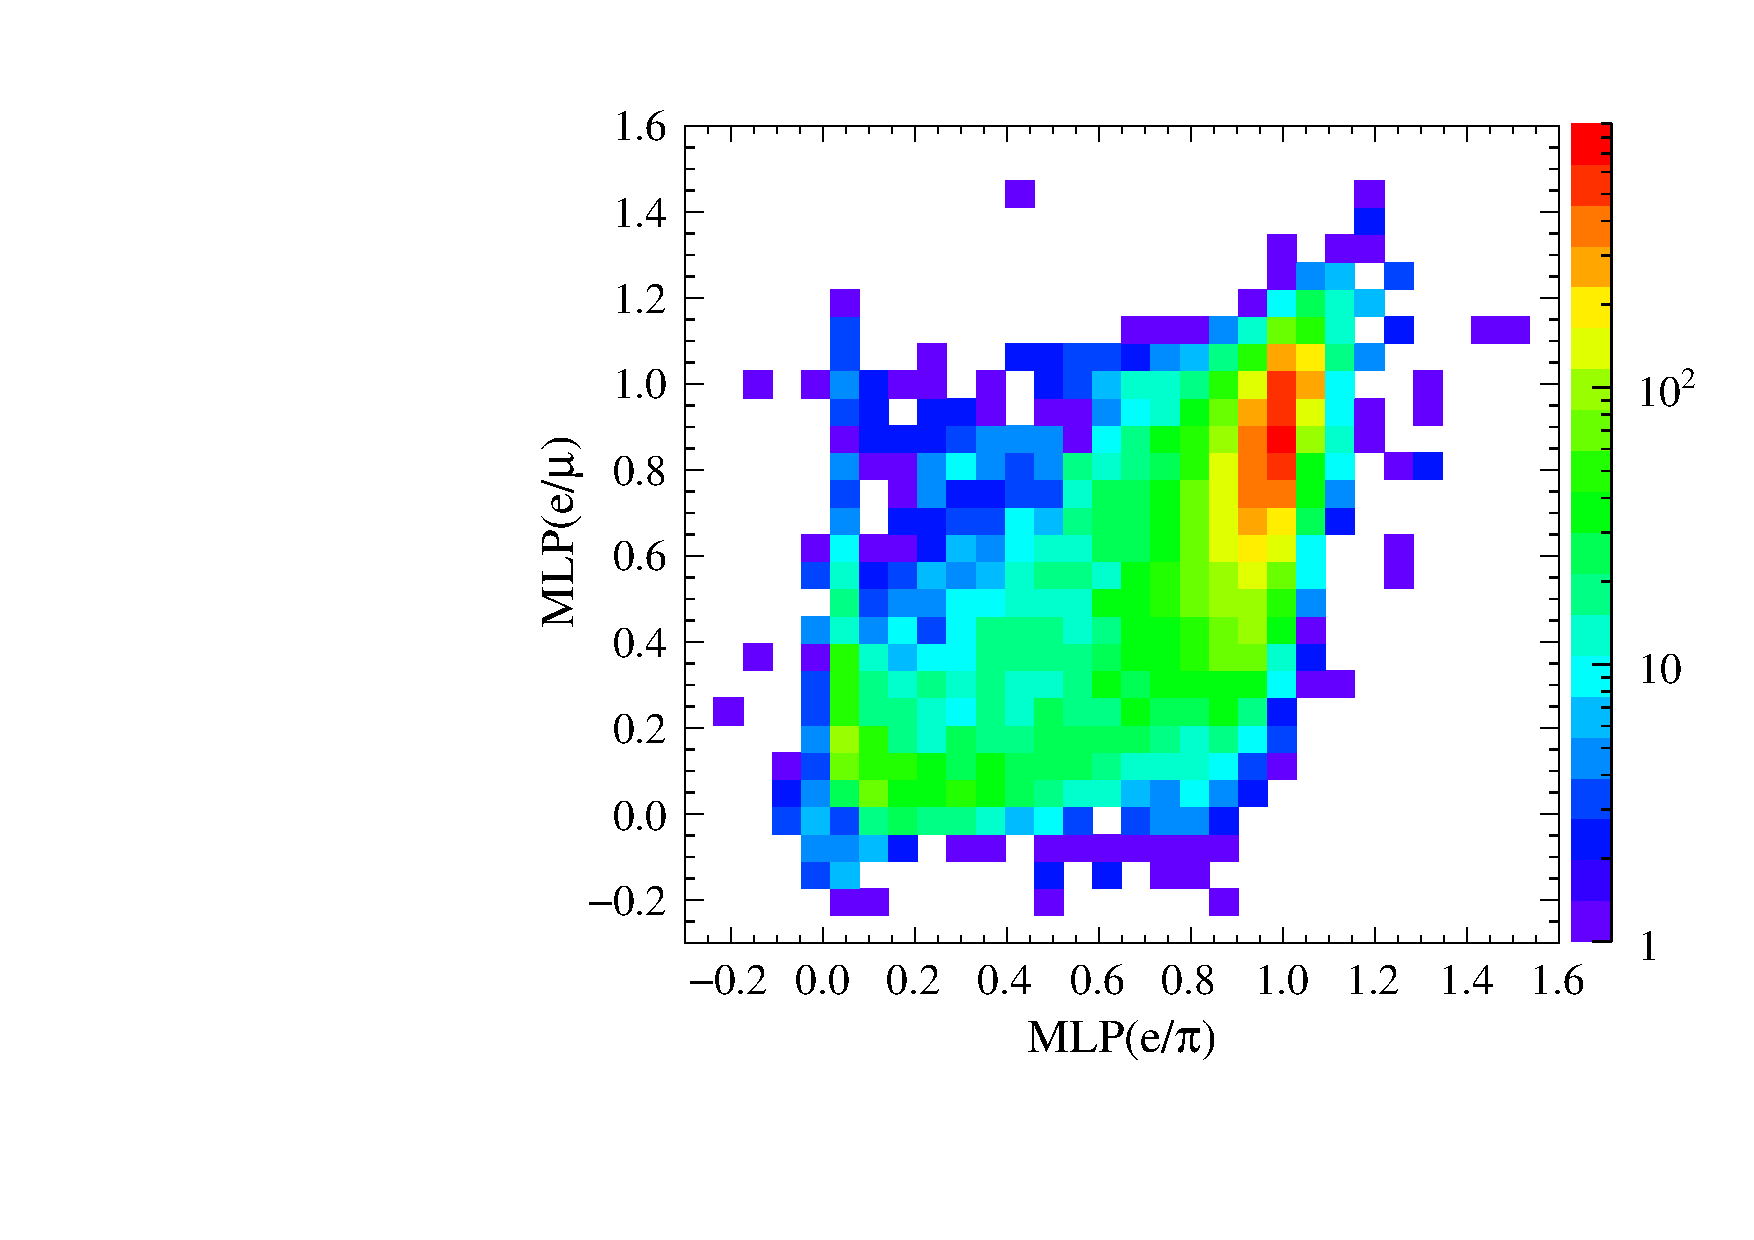
\includegraphics[width=1.0\textwidth]{Chapter7_analysis_kloe/img/csps/emu_vs_epi_data}};
      \draw[black, thick, dashed] (3.5,1.0) -- (1.0,3.5);
    \end{tikzpicture}  
    \caption{All data events}
  \end{subfigure}
  \caption{Relative outputs of the $e/\pi$ and $e/\mu$ classifiers applied to the track identified as electron/positron in the selected event sample. Events are retained if they lie above the dashed line.}\label{fig:mlp_2d}
\end{figure}

After the track and cluster classification described above, the signal to background ratio of the surviving event sample is increased from about 11.3 to 33.5. The contribution of the charge-asymmetric background components $\Ks\to\pi^+\pi^-(\gamma)$ and $\Ks\to\pi^+\pi^-\to\pi\mu\nu$ to the $\Delta t$ distributions used further in this study is strongly reduced as shown in~\fref{fig:csps-dt-after}.

\begin{figure}[h!]
  \captionsetup[subfigure]{justification=centering}
  \centering
  \begin{subfigure}{0.45\textwidth}
  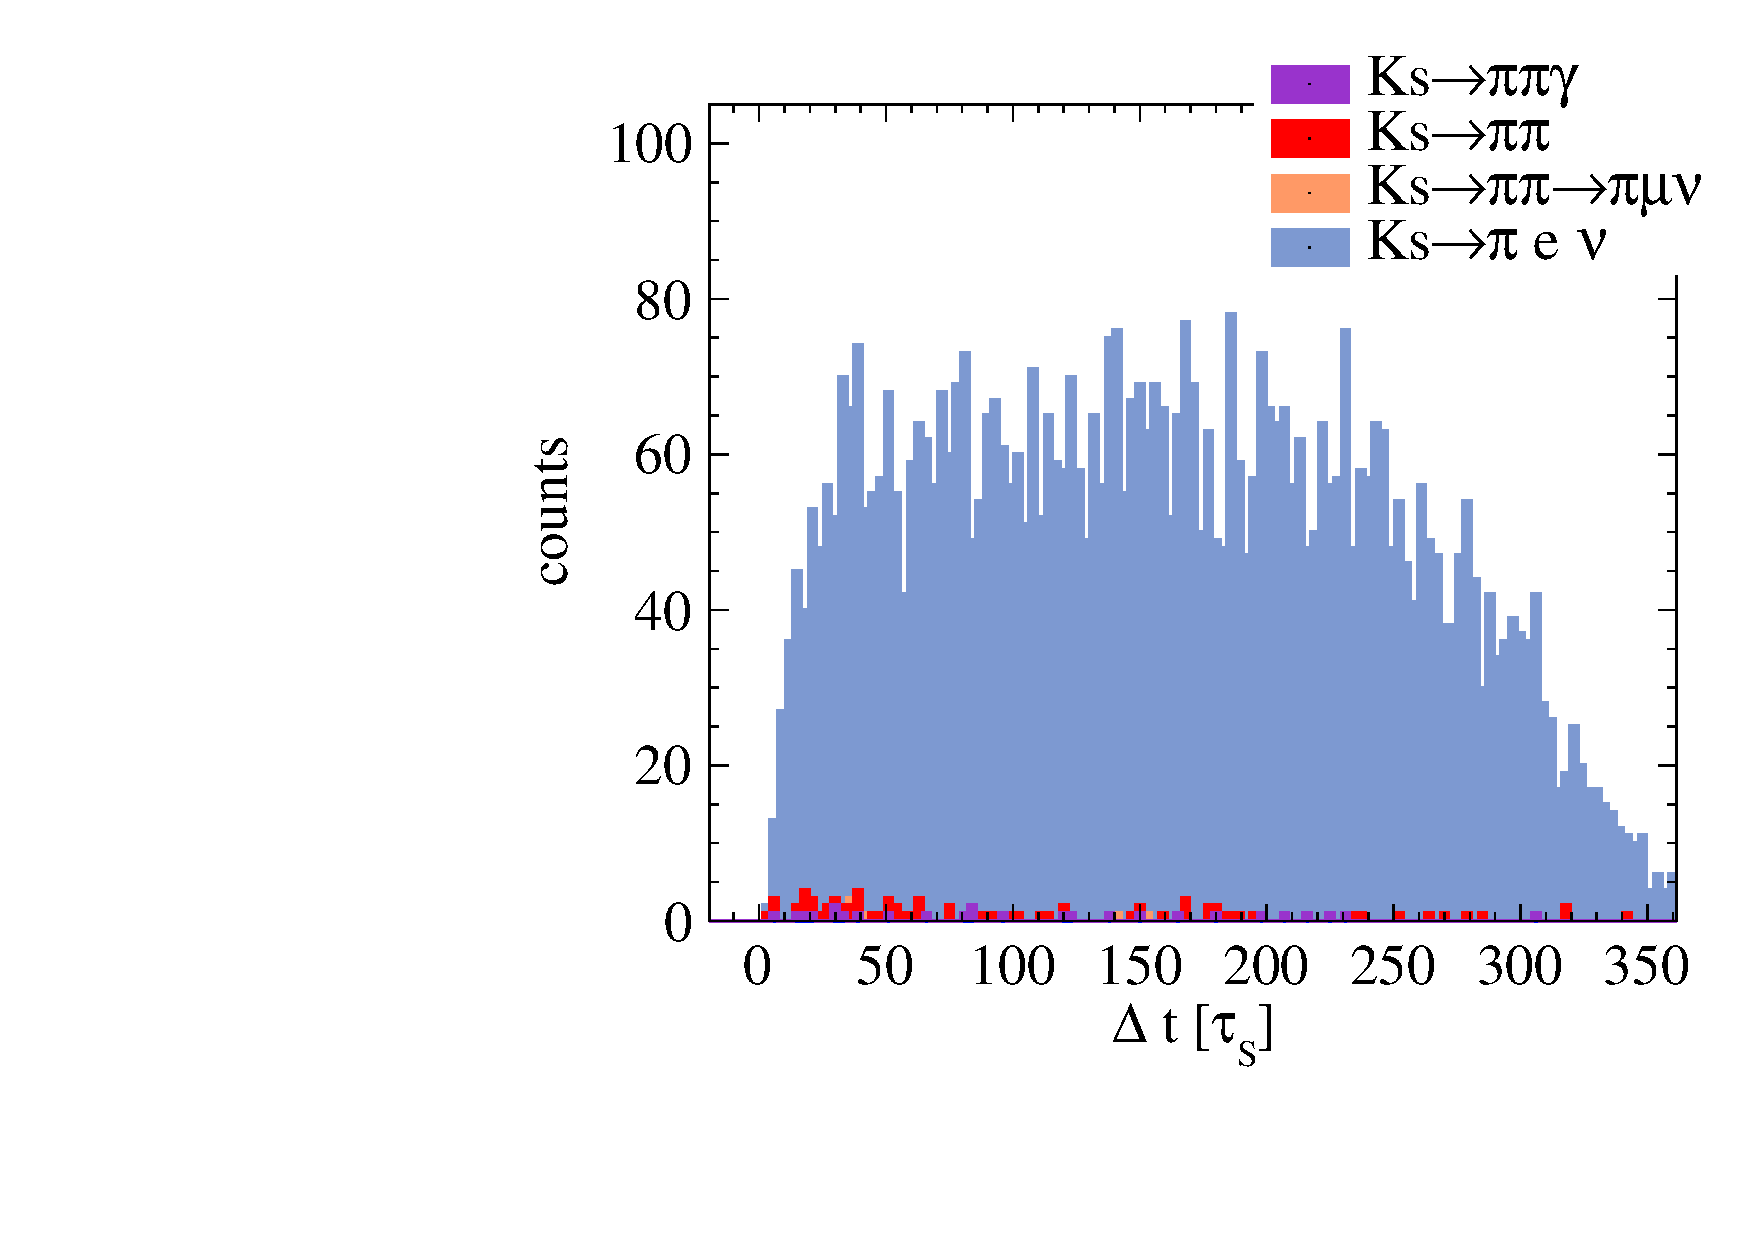
\includegraphics[width=1.0\textwidth]{Chapter7_analysis_kloe/img/csps/no_bcg_eminus}
  \caption{Events with a track identified as electron.}
  \end{subfigure}
  % 
  \begin{subfigure}{0.45\textwidth}
  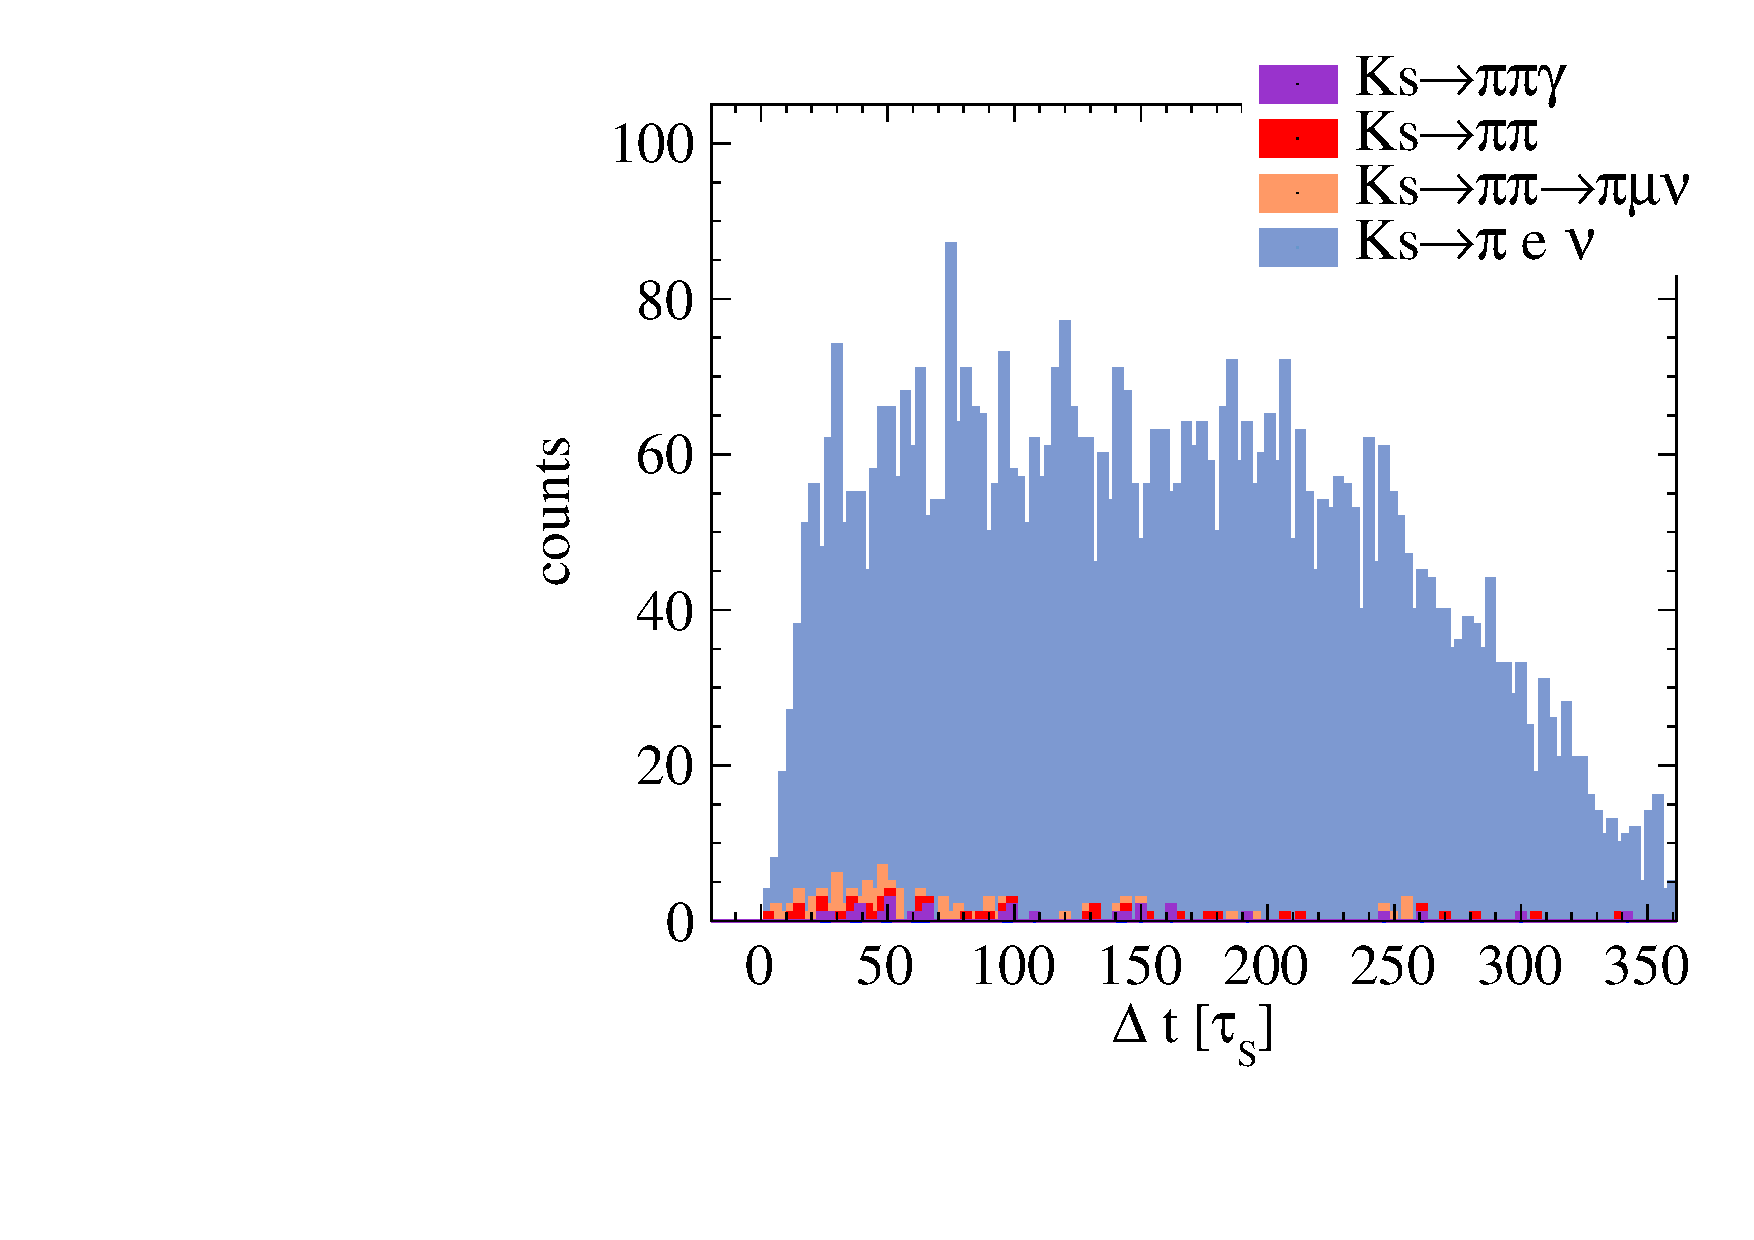
\includegraphics[width=1.0\textwidth]{Chapter7_analysis_kloe/img/csps/no_bcg_eplus}
  \caption{Events with a track identified as positron.}
  \end{subfigure}
  \caption{Stacked MC-based distributions of kaons' decay time difference for signal and background events after application of $e/\pi$ and $e/\mu$ ANN-based track classifiers.}\label{fig:csps-dt-after}
\end{figure}


\subsection{Kinematic fit}\label{sec:kinfit}
A distinctive property of the trilaterative reconstruction of $\Kl\to 3\pi^{0}\to 6\gamma$ decay is its capability to determine the time of decay in addition to vertex position, based predominantly on the event timing. Estimation of decay time based on the distance between the kaon decay and creation point (alike the one performed for the other decay, see~\eref{eq:ks_proper_time}) may therefore be considered as an independent information. Constraining the event topology and timing to enforce equality of both time estimates thus allows for an reduction of the errors on quantities measured in the event, and consequently, for an improvement of the resolution of decay time itself. This aim is achieved with a kinematic fit, in which the following 39 experimentally measured quantities are varied:
\begin{itemize}
\item $x,y,z$, $t$ and $E_{dep}$ for each of the 6 EMC clusters identified as corresponding to the photons from $\Kl\to 3\pi^{0}\to 6\gamma$,
\item 3 Cartesian coordinates of the average $\phi$ decay point,
\item 3 momentum components for each of the two products of the $\Ks\to\pi e\nu$ decay,
\end{itemize}
in order to find a configuration which best satisfies a set of 3 constraints. First constraint is based on the aforementioned agreement between $\Kl$ decay time estimated using trilaterative decay reconstruction ($t_{3\pi^{0}}$) and using the path travelled by the kaon, i.e.:
\begin{equation}
  \label{eq:constraint_vts}
  C_1 = \frac{|\vec{\mathbf{v}}_{3\pi^{0}} - \vec{\mathbf{v}}_{\phi}|}{\upsilon_{K_L}} - t_{3\pi^{0}} = 0,
\end{equation}
where $\vec{\mathbf{v}}_{\phi}$ and $\vec{\mathbf{v}}_{3\pi^{0}}$ are position vectors of the respective vertices and $\upsilon_{K_L}$ is the velocity of the kaon obtained from its momentum.

The second constraint imposed in the kinematic fit requires that invariant mass of the decaying $\Kl$, reconstructed using the momenta of 6 photons, is in agreement with mass of a neutral K meson:
\begin{equation}
  \label{eq:constraint_m6g}
  C_2 = \text{M}(6\gamma) - m_{\kaon} = {\left( \sum_{i=1}^{6} \abs{\vec{p_{\gamma}}^{(i)}} \right)}^2 - \abs{\sum_{i=1}^{6} \vec{p_{\gamma}}^{(i)}}^{2} - m_{\kaon} = 0.
\end{equation}

Finally, the last constraint refers to the semileptonic decay and enforces minimization of the following variable based on the mass attributed to the track identified as electron:
\begin{equation}
  \label{eq:constraint_mtrk}
  C_3 = \text{M}_{trk}^2(e) = \left(E_{\Ks}-E_{\pi}-\abs{\vec{p}_{miss}(\pi,e)}\right)^2 - \abs{\vec{p}_e}^2 = 0,
\end{equation}
where $E_{\Ks}$ and $E_{\pi}$ are the energies of the decaying kaon and the produced charged pion, respectively, $\vec{p}_{miss}(\pi,e)$ is the momentum missing in the decay with an assumption that the products were a charged pion and an electron, and $\vec{p}_e$ is the momentum attributed to the DC track identified as $e^{\pm}$. This variable, expected to be close to zero for semileptonic events, is sensitive to both momentum resolution of the DC tracks corresponding to decay product and to accuracy of $\Ks$ momentum estimation coming from the $\Kl$ decay vertex reconstruction.

The fit was performed as an iterative procedure based on the constrained least squares method~\cite{optimization}. In each step the updated values of measured parameters were used to determine new estimates of the $\Kl\to 3\pi^0$ decay vertex and time with the trilaterative technique, and, subsequently, new estimates of both kaons' momenta were calculated using the procedure described in~\sref{sec:ks_from_kl}. Only then were the values of the constraints recalculated and a set of corrections $\mathbf{\Delta x}$ to the vector of measured quantities $\mathbf{x}$ was found which minimizes the following $\chi^2$-like function:
\begin{equation}
  \label{eq:general_chisq}
  \chi^2 = \mathbf{\Delta x}^T \mathbf{V}^{-1} \mathbf{\Delta x} + \mathbf{\lambda}^T(\mathbf{D\Delta x} + \mathbf{C}(\mathbf{x})),
\end{equation}
where $\mathbf{V}$ is a covariance matrix of the varied parameters, $\mathbf{\lambda}$ is a vector of Lagrange multipliers, $\mathbf{D}$ denotes a matrix of derivatives of the constraints $C_{1-3}$ over the varied parameters, and $\mathbf{C}$ stands for a vector of constraint values at point $\mathbf{x}$ in the parameter space.
%The exact recipe for the minimization procedure used in the kinematic fit is described in~\aref{appendix:kinfit}.

\begin{figure}[h!]
  \centering
  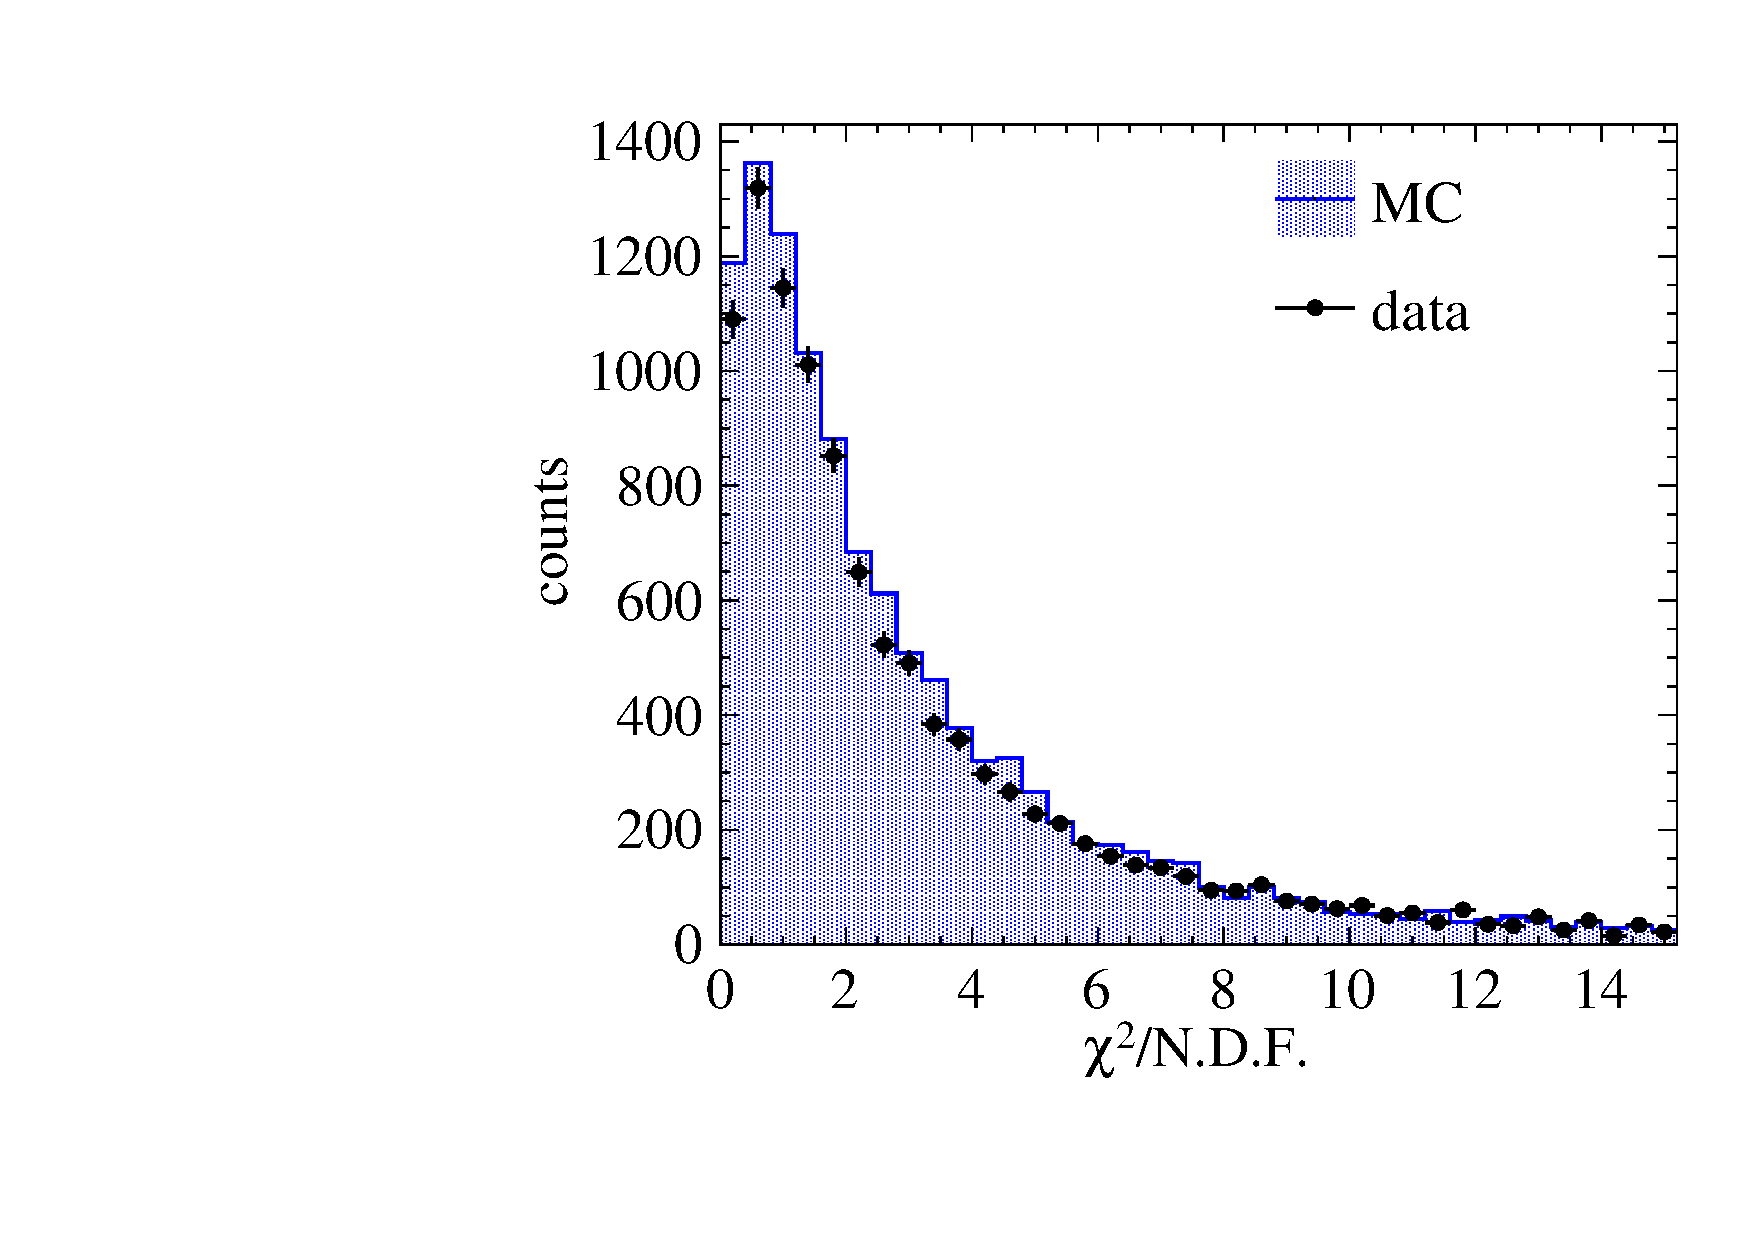
\includegraphics[width=0.45\textwidth]{Chapter7_analysis_kloe/img/chisq}
  \caption{Distribution of $\chi^{2}$ normalized to the number of degrees of freedom resulting from the kinematic fit.}\label{fig:chisq}
\end{figure}

The kinematic fit was applied to all events surviving the selection steps described in the previous Sections. The reason for its introduction at this stage is that the first constraint~(\eref{eq:constraint_vts}), crucial for improvement of reconstruction of $\Kl$ travelled path length and decay time, relies on measurement of the 6 photons' interaction time in the KLOE EMC with a correct event start time, which is only determined after the time of flight analysis.

\begin{figure}[h!]
  \centering
  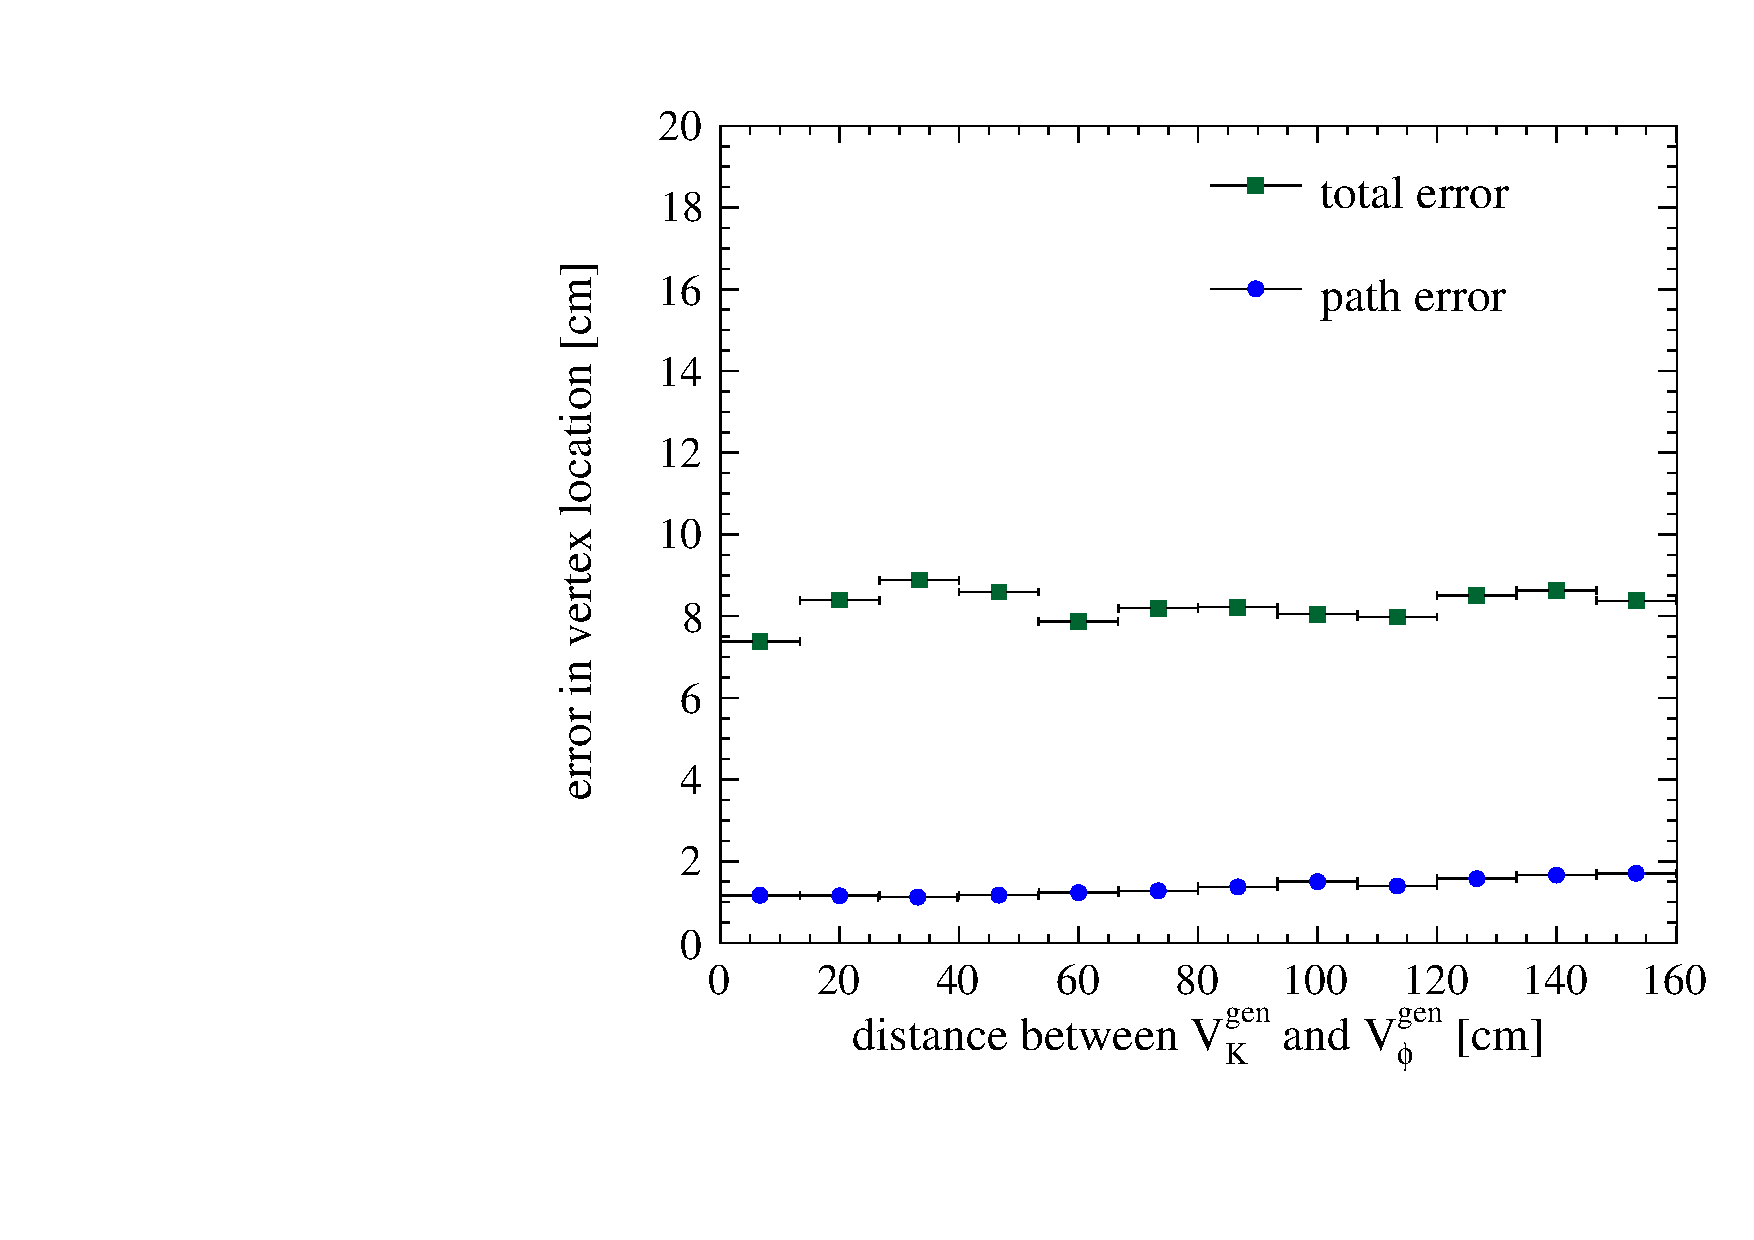
\includegraphics[width=0.45\textwidth]{Chapter7_analysis_kloe/img/resolution_fit}
  \hspace{1em}
  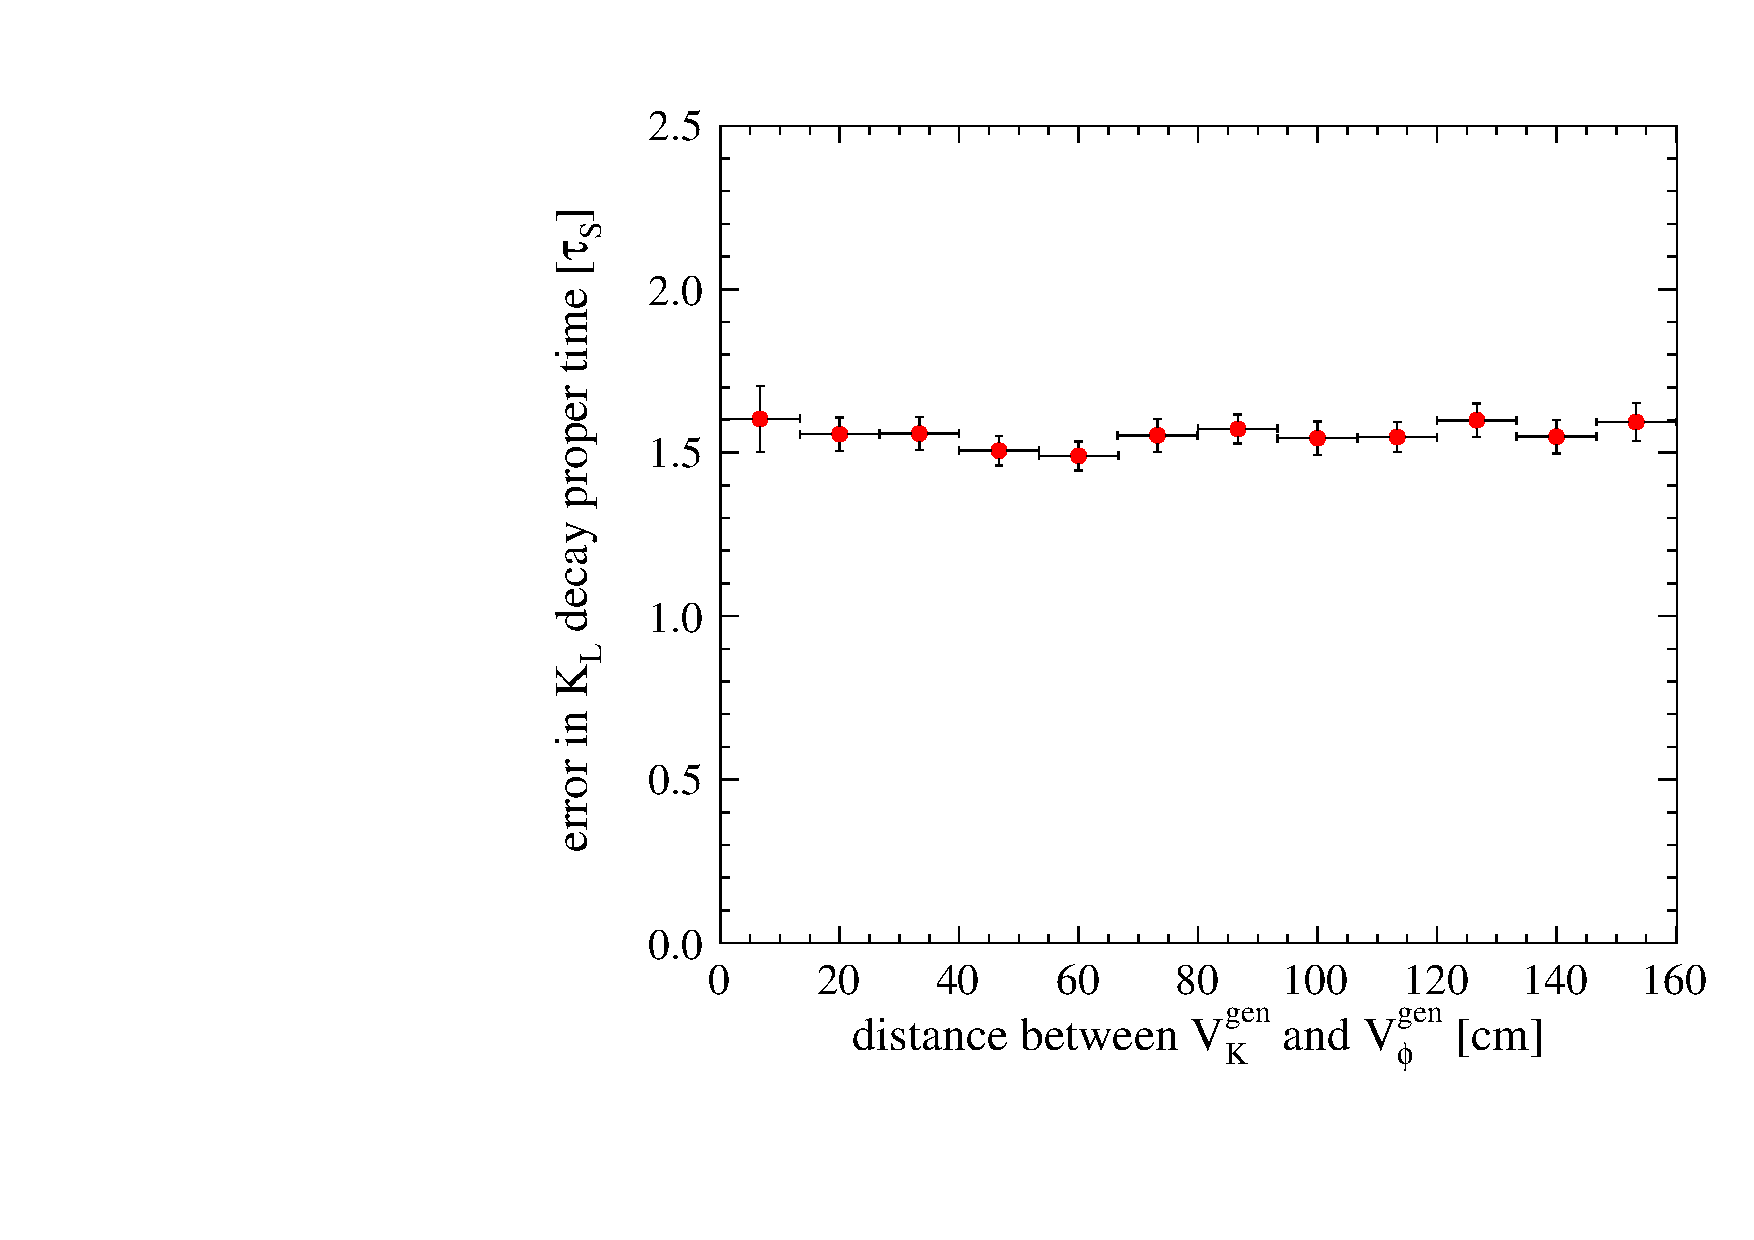
\includegraphics[width=0.45\textwidth]{Chapter7_analysis_kloe/img/resolution_t_fit}
  \caption{MC-based study of the resolution of reconstructed $\Kl\to 3\pi^0$ decay position (left) and proper time (right) obtained after the kinematic fit. Resolution is defined as $\sigma$ of an error on reconstructed w.r.t.\ MC-generated decay in subsequent ranges of decay distance from $\phi$.}\label{fig:resolution_fit}
\end{figure}

\fref{fig:chisq} presents a distribution of minimal $\chi^{2}$ values obtained with the procedure described above, normalized to the number of degrees of freedom in the fit. The agreement between data and MC-simulated events indicates similar performance of the fitting procedure in both cases. The resolution of $\Kl\to 3\pi^0$ decay point and time obtained after the kinematic fit was studied with a MC sample in a similar manner as for the reconstruction without the fit (see~\sref{sec:kl3pi0}). The resulting resolution of the spatial vertex location and proper decay time of the kaon is shown in the left and right panels of~\fref{fig:t2-kspipi}, respectively. The improvement of of spatial reconstruction, especially of the length of the path travelled by the kaon (compare~\fref{fig:resolutions_nofit}) leads to a resolution of the $\Kl$ decay proper time at the level of approximately~1.6~$\tau_S$ independently of the location of the decay in the KLOE detector~\cite{gajos-acta,Gajos:2015ija}. According to Monte Carlo-simulation studies, this resolution combined with the one of $\Ks\to \pi e \nu$ decay time reeults in the resolution of both decays' time difference $\Delta t$ at the level of 2.3~$\tau_S$. Consequently, in the further considerations of any distributions as functions of $\Delta t$, a bin width of 3~$\tau_S$ is used.
%
% TODO: wyrysowac rozdzielczosc delta t i uzasadnic dlaczego wybrane binowanie 3 tau_s
% 
\section{Selection and reconstruction of the $\Ks \Kl \to \pi^{+}\pi^{-} \pi^{\pm}e^{\mp}\nu$ process}\label{sec:t-analysis-2}

The process where an earlier kaon decays into two charged pions and the later one through a semileptonic channel requires a more straightforward event selection than $\Ks\Kl\to\pi e\nu\;3\pi^0$, mostly due to the fact that the combined branching ratio of the required decays amounts to about \SI{28}{\percent}, over 2000 times larger than in case of the other class of processes. Moreover, the $\Ks\to\pi^+\pi^-$ decay is well identified by tracks of both products recorded by the KLOE drift chamber, whose sum of momenta additionally provides a precise estimate of $\vec{p}_{\Ks}$.

\subsection{Selection of $\Ks$ decays into charged pions}\label{sec:kspipi}
Similarly as in the case of the first class of events (see~\sref{sec:t-analysis-1}), the selection of $\Ks \Kl \to \pi^{+}\pi^{-} \pi e\nu$ process is started at the level of the neutral kaon stream of KLOE data and corresponding Monte Carlo-simulated events. As a first criterion, presence of two tracks in the drift chamber is required which share a common vertex located within a cylindrical volume limited by $r_T<$15~cm and $|z|<$10~cm, where a majority of $\Ks$ decays are expected. In the process of interest, however, the decay vertex of an early semileptonic decay of the long-lived neutral kaon can satisfy the same requirement. To avoid confusing the vertices in signal events, for all 2-track vertices located in the fiducial volume for $\Ks$ decays the invariant mass of decaying kaon M$(\pi,\pi)$ is reconstructed using product tracks with an assumption that both correspond to charged pions. If more than one such vertex is present, the one is selected for which the calculated invariant mass is closest to the neutral kaon mass.

Distribution of the invariant masses for the selected 2-track decay vertices is shown in the left panel of~\fref{fig:t2-kspipi}. As evident from the MC-simulated spectra, for the $\Ks\to\pi^+\pi^-$ recorded tracks of the produced pions yield an accurate estimate of the decaying kaon mass and thus a highly pure set of these events is obtained with the following cut on the reconstructed invariant mass with $\pi^+\pi^-$ mass assumption:
\begin{equation}
  \label{eq:t2-invmass-cut}
  \abs{\text{M}(\pi,\pi) - m_{\kaon}} < 10\:\text{MeV}.
\end{equation}

\begin{figure}[h!]
  \centering
  \begin{tikzpicture}
    \node[anchor=south west,inner sep=0] at (0,0) 
    {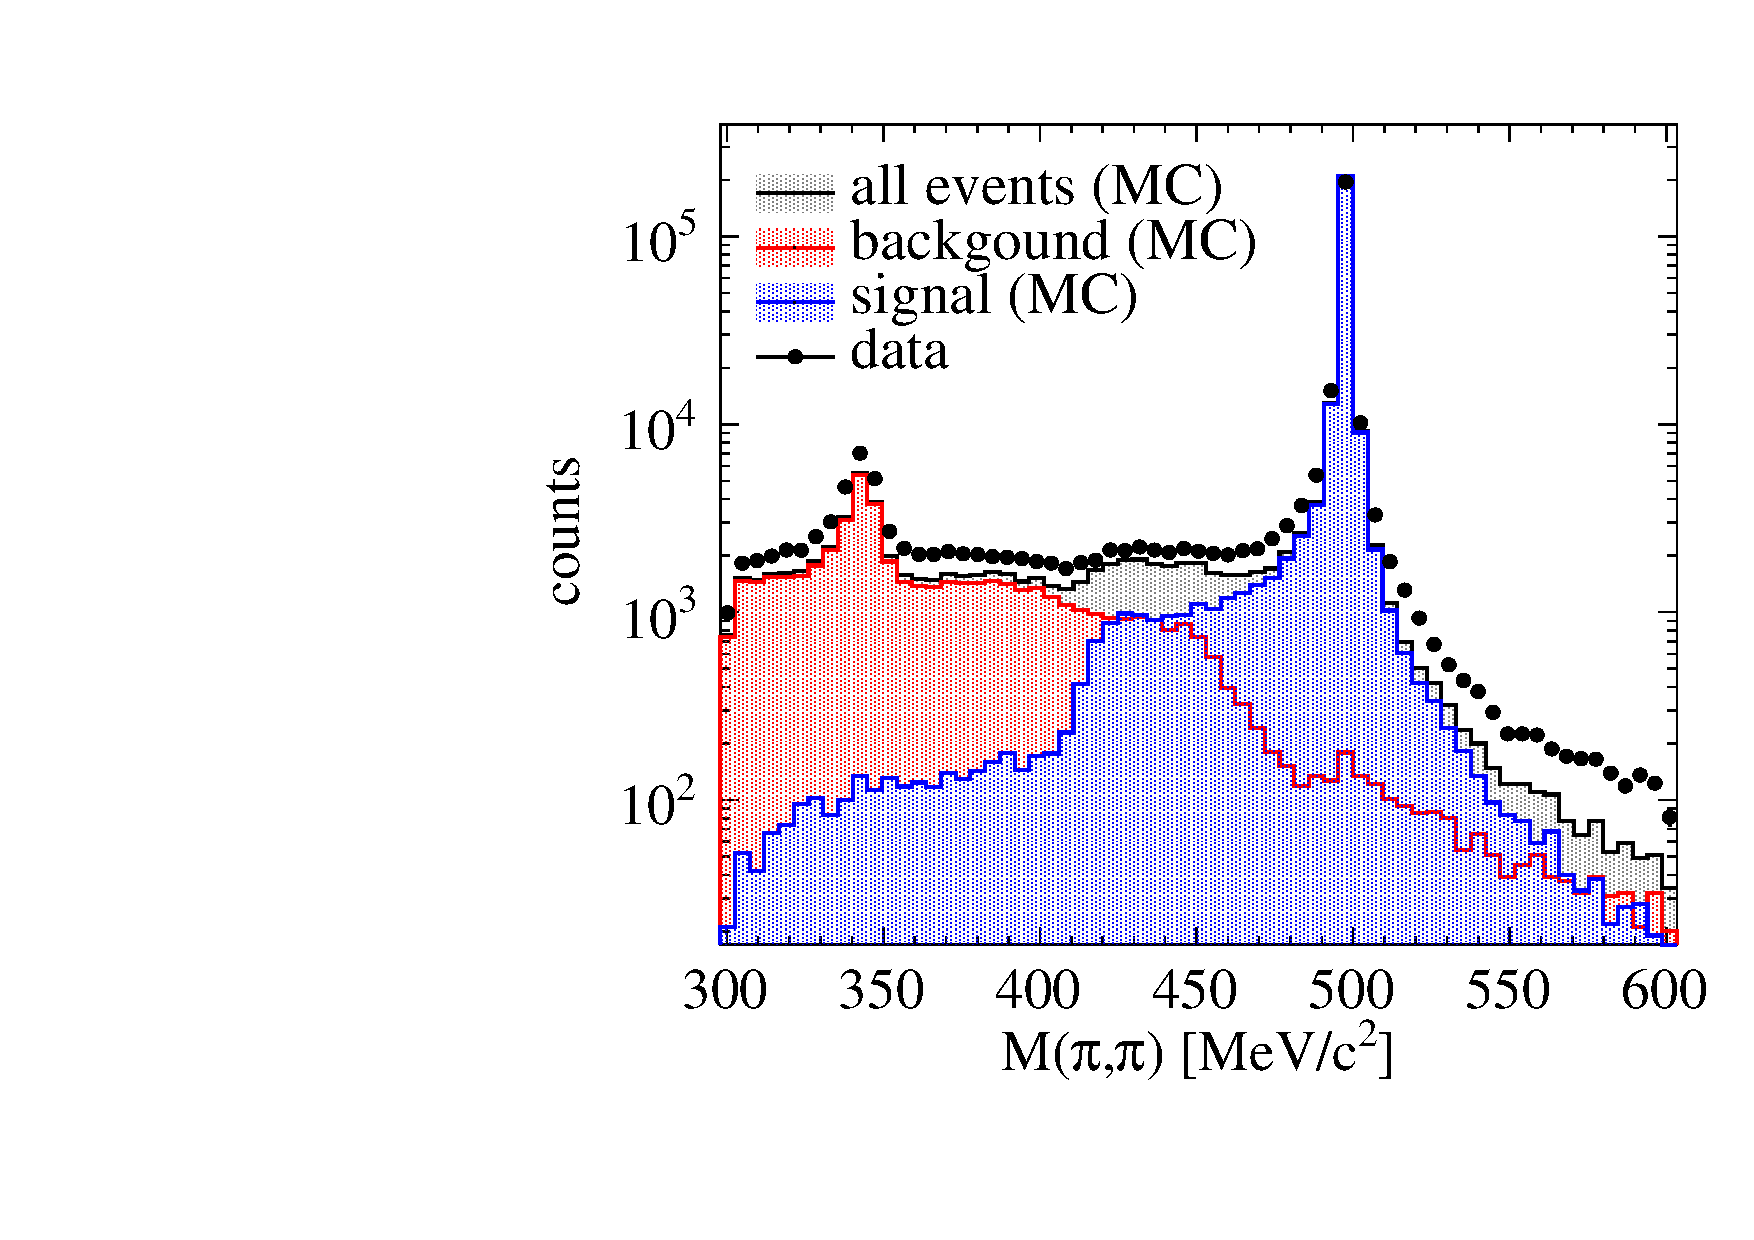
\includegraphics[width=0.45\textwidth]{Chapter7_analysis_kloe/img/t2/invmass_ks}};
    \draw[black, thick, dashed] (4.47,0.8) -- (4.47,5.46);
    \draw[black, thick, dashed] (4.85,0.8) -- (4.85,5.46);
    \draw[ultra thick, black!70!white, <->] (4.44, 1.2) -- (4.87, 1.2);
  \end{tikzpicture}
  \hspace{1em}
  \begin{tikzpicture}
    \node[anchor=south west,inner sep=0] at (0,0) 
    {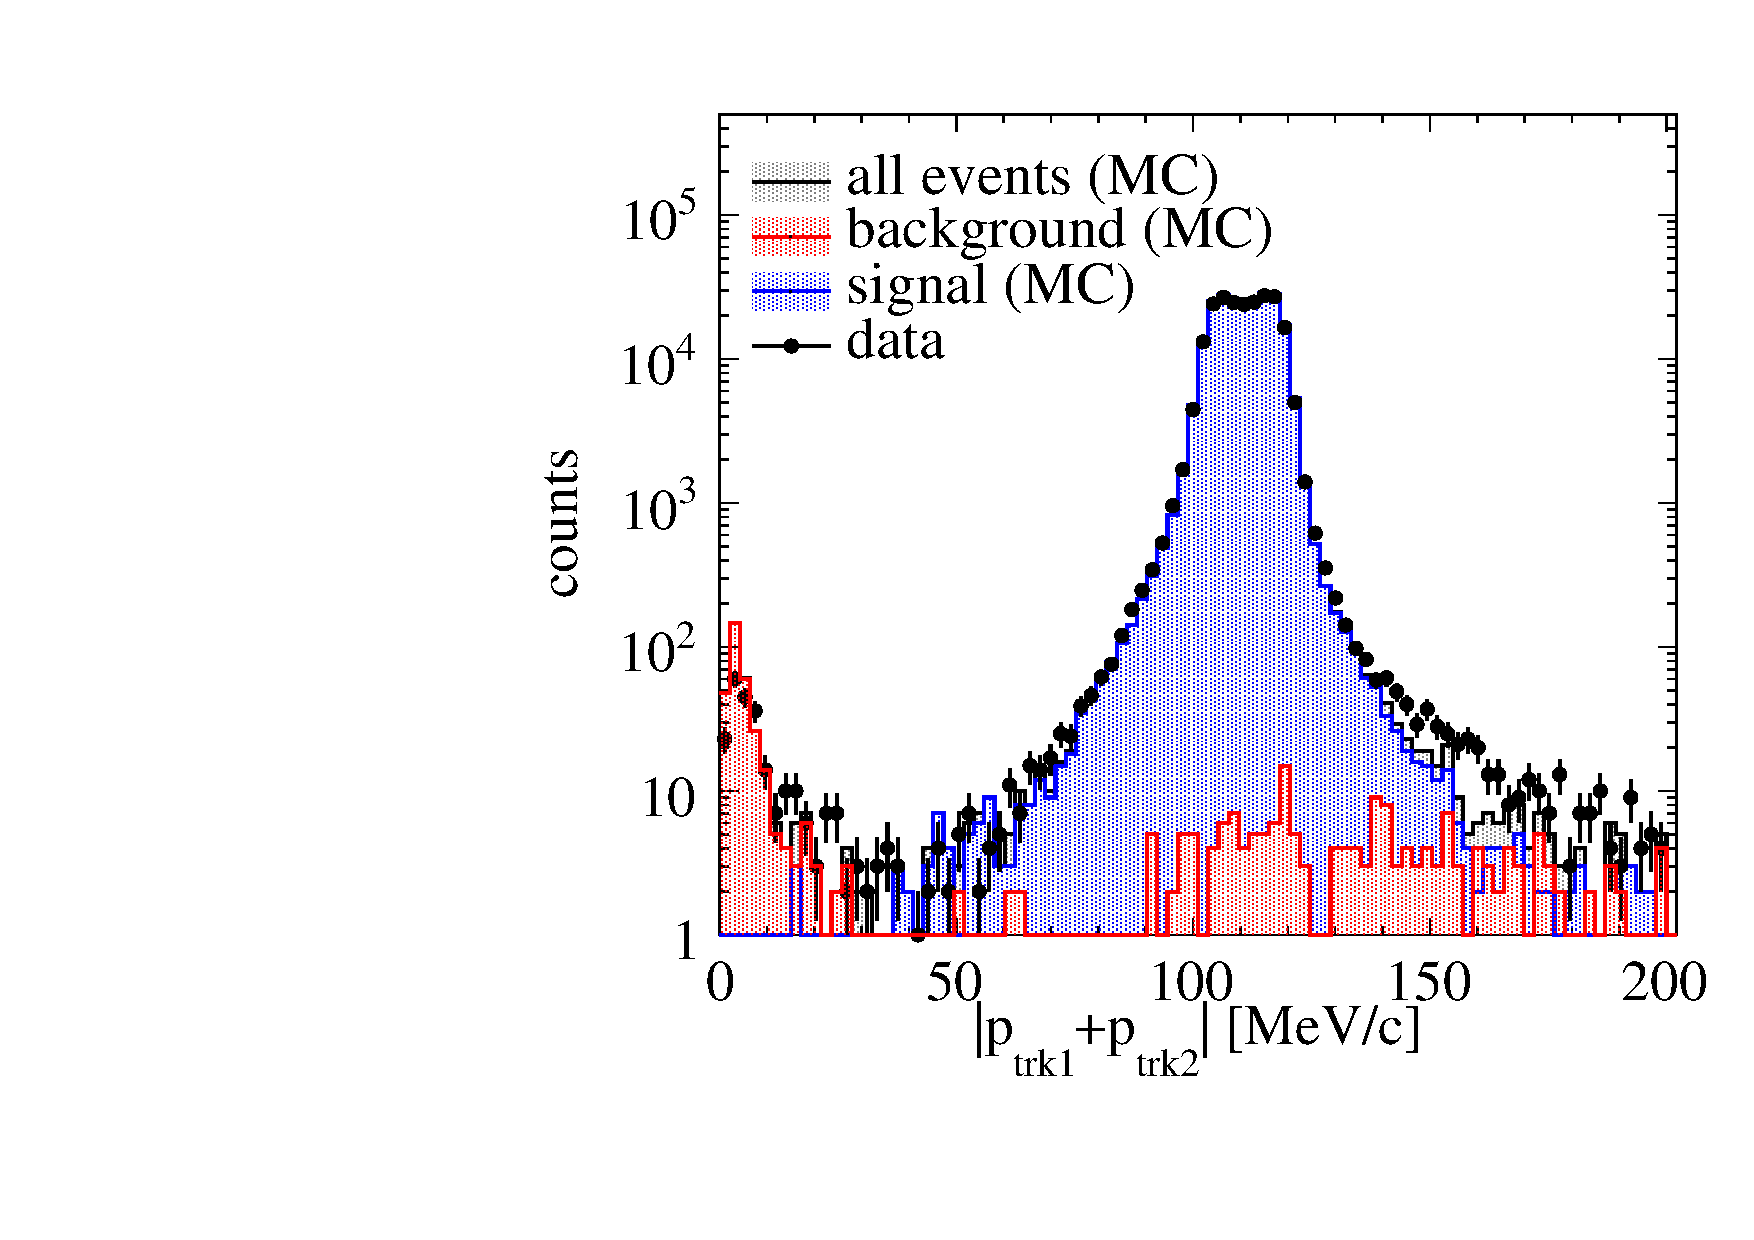
\includegraphics[width=0.45\textwidth]{Chapter7_analysis_kloe/img/t2/ptot_ks}};
    \draw[black, thick, dashed] (3.4,0.8) -- (3.4,4.0);
    \draw[black, thick, dashed] (4.75,0.8) -- (4.75,5.46);
    \draw[ultra thick, black!70!white, <->] (3.42, 2.2) -- (4.73, 2.2);
  \end{tikzpicture}
  \caption{Left: invariant mass of a decaying kaon reconstructed with momenta corresponding to the two DC tracks assuming both were charged pions. Right: Sum of momenta corresponding to the two DC tracks after a cut on the $\pi,\pi$ invariant mass. Dashed lines denote values of the cuts used and gray arrows indicate the accepted regions.}\label{fig:t2-kspipi}
\end{figure}

Subsequently, the sum of momenta associated with the two DC tacks is restricted to be close to the nominal momentum modulus of a neutral kaon originating from a $\phi$ decay from the DA$\Phi$NE collider which amounts to about 110~MeV/c:
\begin{equation}
  \label{eq:t2-ptot-cut}
  \abs\Big{\abs{\vec{p}_{trk1} + \vec{p}_{trk2}} - 110\:\text{MeV/c}} < 25\:\text{MeV/c}.
\end{equation}
Although this cut only removes a small amount of background surviving the invariant mass cut as shown in the right panel of~\fref{fig:t2-kspipi}, its purpose is also to limit the further analysis to events with well reconstructed momenta of the pions.

\subsection{Selection of $\Kl\to \pi^{\pm}e^{\mp}\nu$ decays}\label{sec:klsemil}
Semileptonic decays of the long-lived neutral K meson may be identified by analyzing the times of flight of products particles from the decay point to their incidence on the calorimeter, in a similar manner as in case of $\Ks\to\pi e \nu$ (\sref{sec:t1_tof}). Preparation of a high-purity event sample is easier in this case due to considerably larger branching fraction for semileptonic decays of $\Kl$ (see~\tref{tab:kaon_properties}). A major difference, however, is that the kaon decay may occur anywhere inside the detector. In presence of background processes, this may require selecting a correct vertex among several decay vertices recorded by the drift chamber in a single event.

Previous analyses of $\Kl\to\pi e\nu$ at KLOE~\cite{kloe_memo_280,kloe_memo_322,kloe_memo_334,kloe_kl3pi0_br} utilized the accurate estimate of $\Kl$ momentum direction obtained from $\Ks\to\pi^+\pi^-$ and momentum conservation in the $\phi$~decay to search for a 2-track DC vertex closest to the $\Kl$ line of flight.
%
% TODO: dodac ref do sekcji z opisem kanalu kontrolnego z Ks->pi0pi0
%
Such approach, however, is not feasible in case of the analysis presented in this work as the channel which is later used as a control sample for estimation of selection efficiency of $\Kl\to\pi e \nu$ is a process where the latter is accompanied by a $\Ks\to\pi^0\pi^0$ decay. In such case, the accuracy of $\vec{p}_{\Ks}$ obtained from photons' momenta is considerably lower, resulting in poor angular resolution of $\Kl$ line of flight and a  degradation of selection efficiency. Therefore, in this analysis, an alternative approach was devised which does not rely on momentum estimation obtained form the other kaon in the same event.

In order to find the decay vertex and tracks corresponding to an electron/positron and to a charged pion, all vertices constituted by two tracks in the drift chamber were considered as candidates with an exception of the previously identified vertex of $\Ks\to\pi^+\pi^-$. As the pions may decay in the DC, vertices connected to tracks associated to $\pi^+\pi^-$ from the $\Ks$ decay were also excluded. Multiplicity of vertex candidates is shown as a black histogram in~\fref{fig:klvtxcount}. In order to reduce the ambiguity of vertex choice,
for each of the candidates 
an extrapolation to the inner surface of the calorimeter was attempted
for its two associated DC tracks. If a successful extrapolation was followed by finding a corresponding EMC cluster for both tracks, the vertex was considered in further analysis and rejected otherwise. After this step, the amount of events with more than one vertex candidate was still at the level of several percent as shown by the blue histogram in~\fref{fig:klvtxcount}. Therefore, each of the surviving candidates was subject to a time of flight analysis.

\begin{figure}[h!]
  \centering
  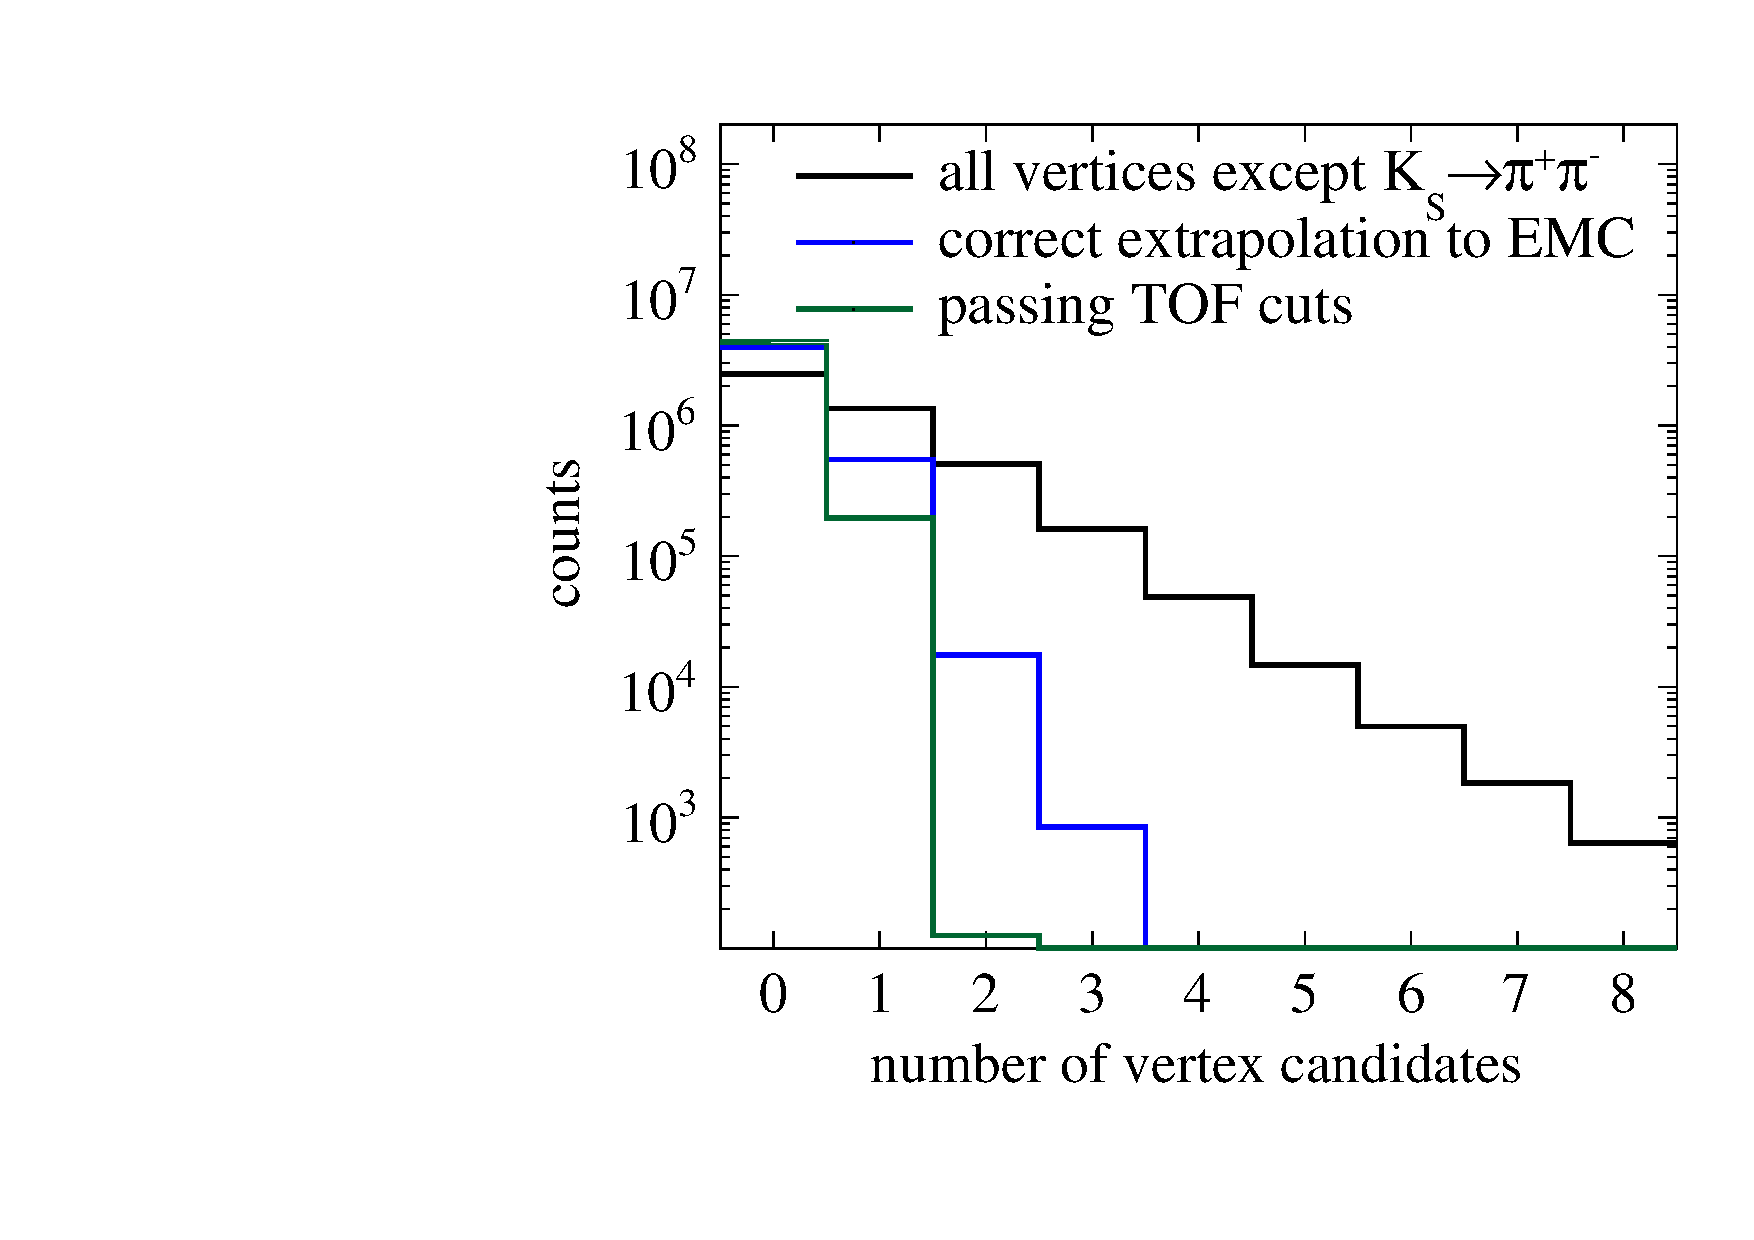
\includegraphics[width=0.45\textwidth]{Chapter7_analysis_kloe/img/t2/klvtxcount}
  \caption{Multiplicity of $\Kl$ decay vertex candidates, ie.\ all vertices except the one identified as $\Ks\to\pi^+\pi^-$ and subsequent pion decays (black), vertices for which both associated tracks were correctly extrapolated to the EMC surface and associated to a cluster (blue) and vertices for which the particles associated to the tracks passed the time of flight cuts (green). Distributions were obtained with data.}
  \label{fig:klvtxcount}
\end{figure}

The TOF analysis applied to the 2 tracks associated with each vertex candidate was similar to the one used for $\Ks\to\pi e\nu$ (see~\sref{sec:t1_tof}). Again, the difference between recorded time of flight (based on the EMC cluster registration time) and the time expected from particle path length along the extrapolated DC track and its velocity, was used to define the variables of the TOF analysis. In case of $\Kl$ decays, however, the expected time of flight included an additional component related to the flight of the kaon before its decay,~$\frac{L_K}{\upsilon_K}$:
\begin{equation}
  \label{eq:dtof_t2}
  \delta t({m_x}) = t_{cl} - \frac{L}{c\beta(m_x)}  - \frac{L_K}{\upsilon_K},
\end{equation}
where $L_K$ is the distance from the average $\phi$ decay point to the location of considered $\Kl$ decay vertex candidate, and $\upsilon_K$ is the kaon velocity obtained from its momentum.

In order to avoid any dependency of the TOF analysis on resolution of $\Ks$ momentum (with a view to its application on a $\Ks\Kl\to\pi^0\pi^0\;\pi e\nu$ control sample), the $\abs{\vec{p}_{\Kl}}$ value was calculated using momentum conservation in the $\phi\to\Ks\Kl$ decay as described in~\sref{sec:ks_from_kl} by assuming that the $\Kl$ momentum direction was parallel to the kaon path spanning between the $\phi$ vertex and current vertex candidate.

\begin{figure}[h!]
  \captionsetup[subfigure]{justification=centering}
  \centering
  \begin{subfigure}{0.45\textwidth}
    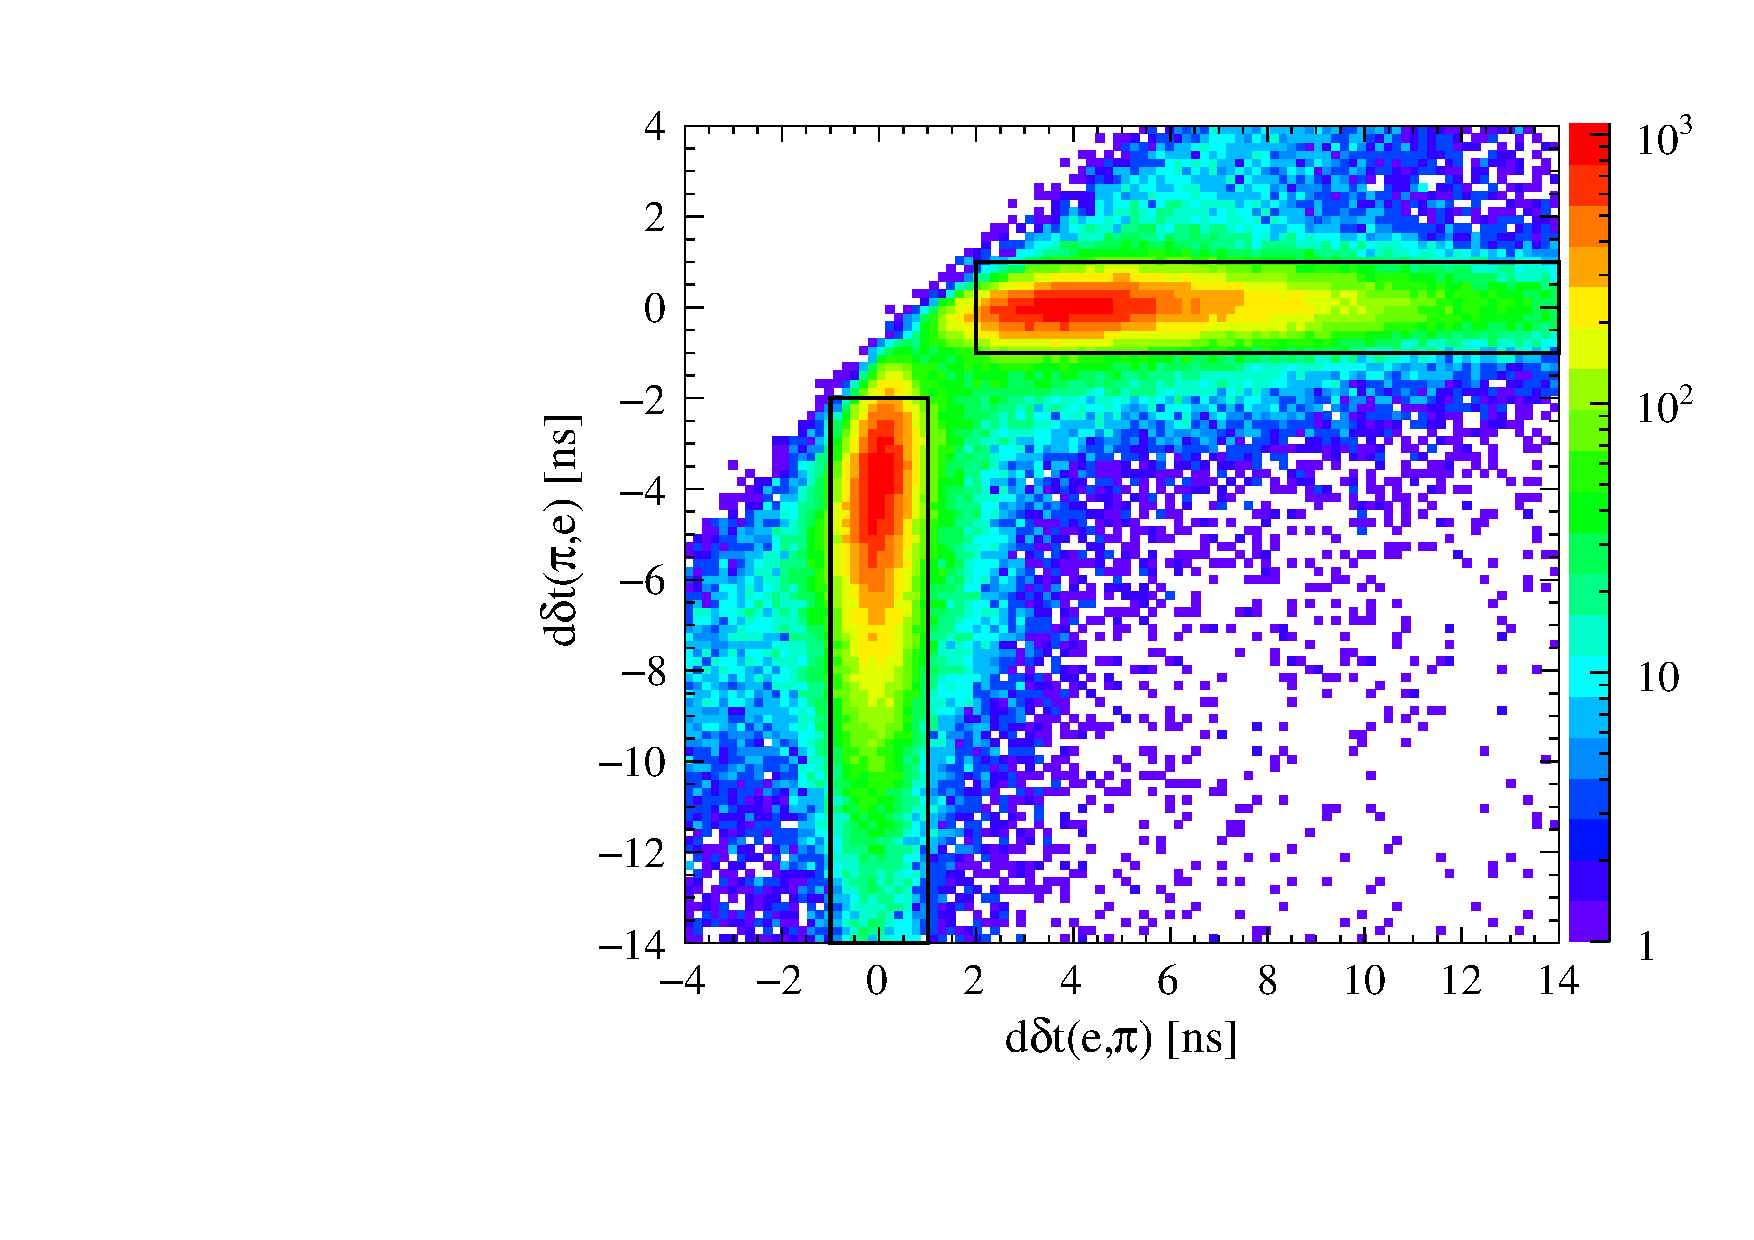
\includegraphics[width=1.0\textwidth]{Chapter7_analysis_kloe/img/t2/t2_tof1_signal}
    \caption{Signal events (MC)}
  \end{subfigure}
  %
  \begin{subfigure}{0.45\textwidth}
    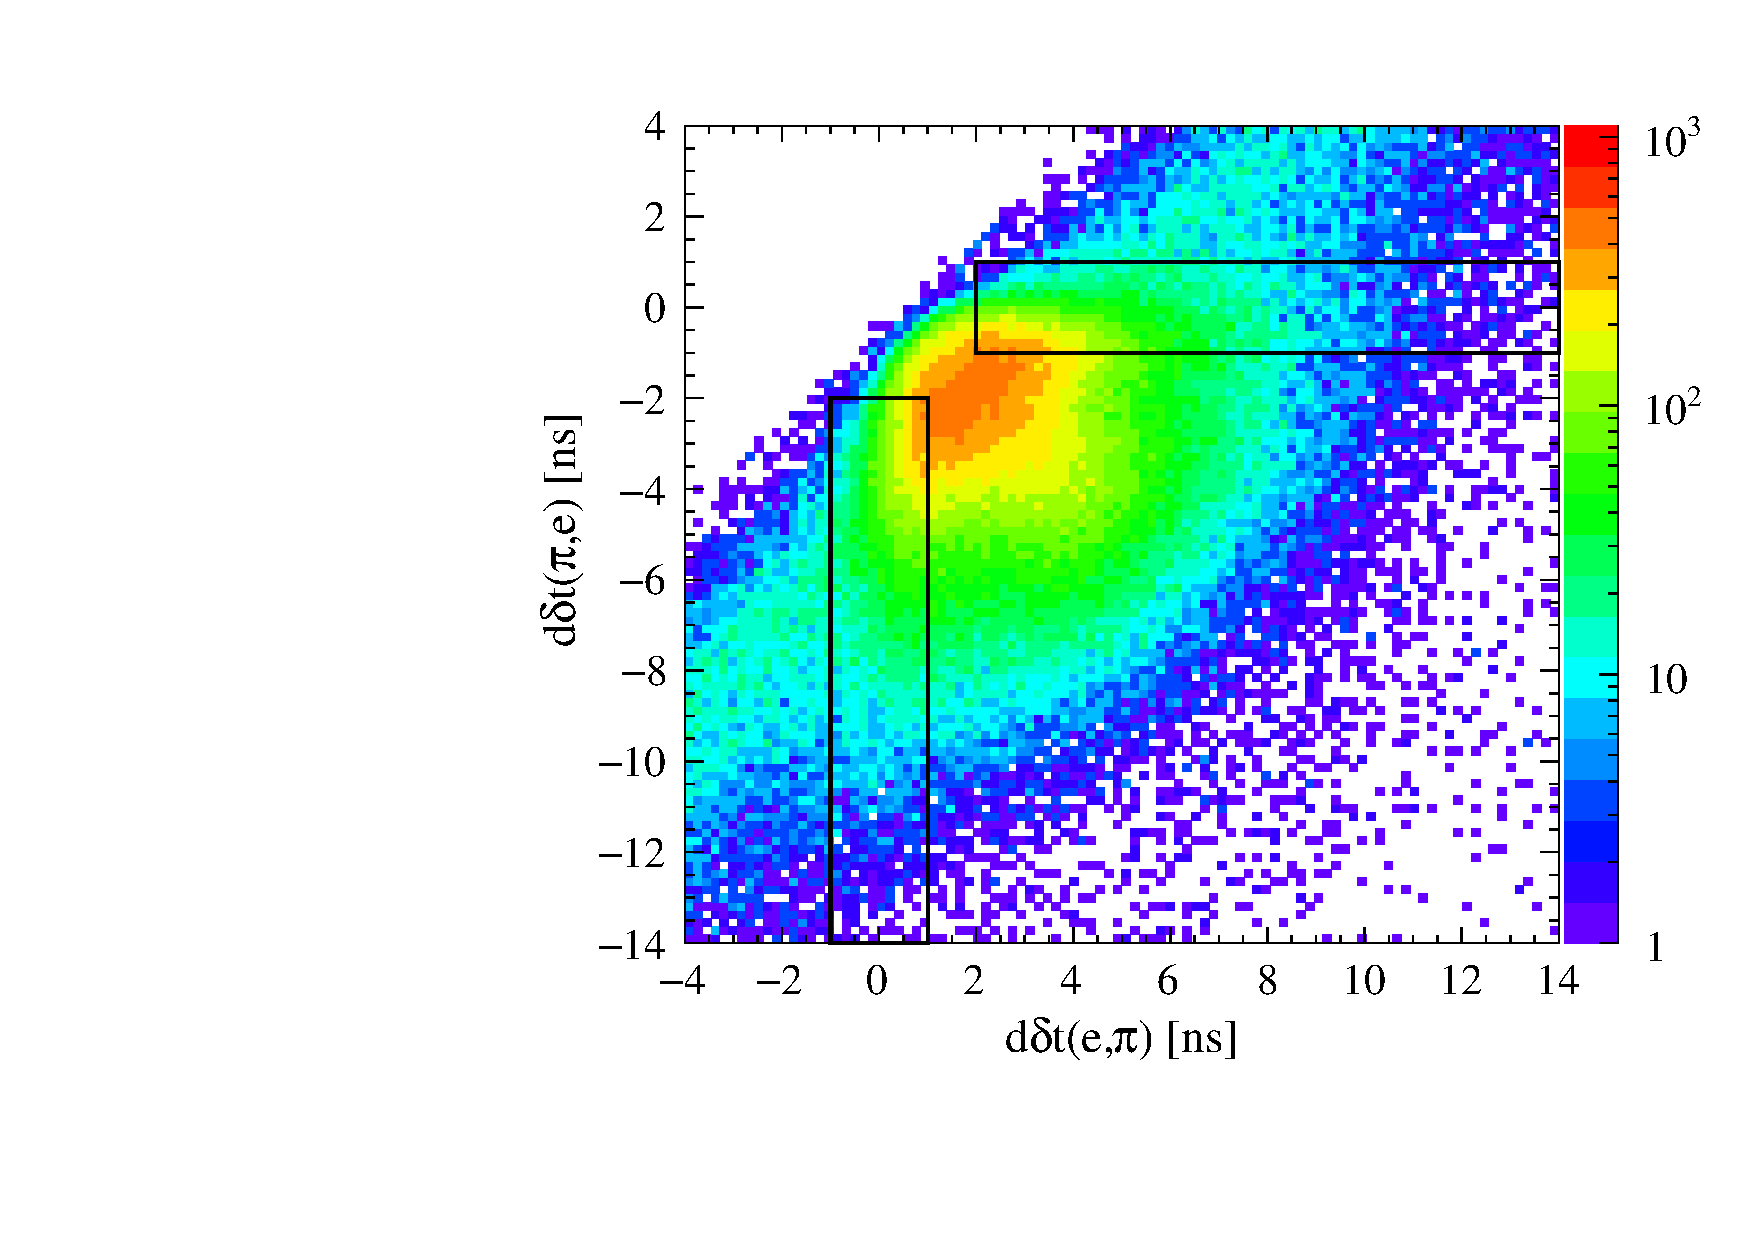
\includegraphics[width=1.0\textwidth]{Chapter7_analysis_kloe/img/t2/t2_tof1_background}
    \caption{Background events (MC)}
  \end{subfigure}
  %
  \begin{subfigure}{0.45\textwidth}
    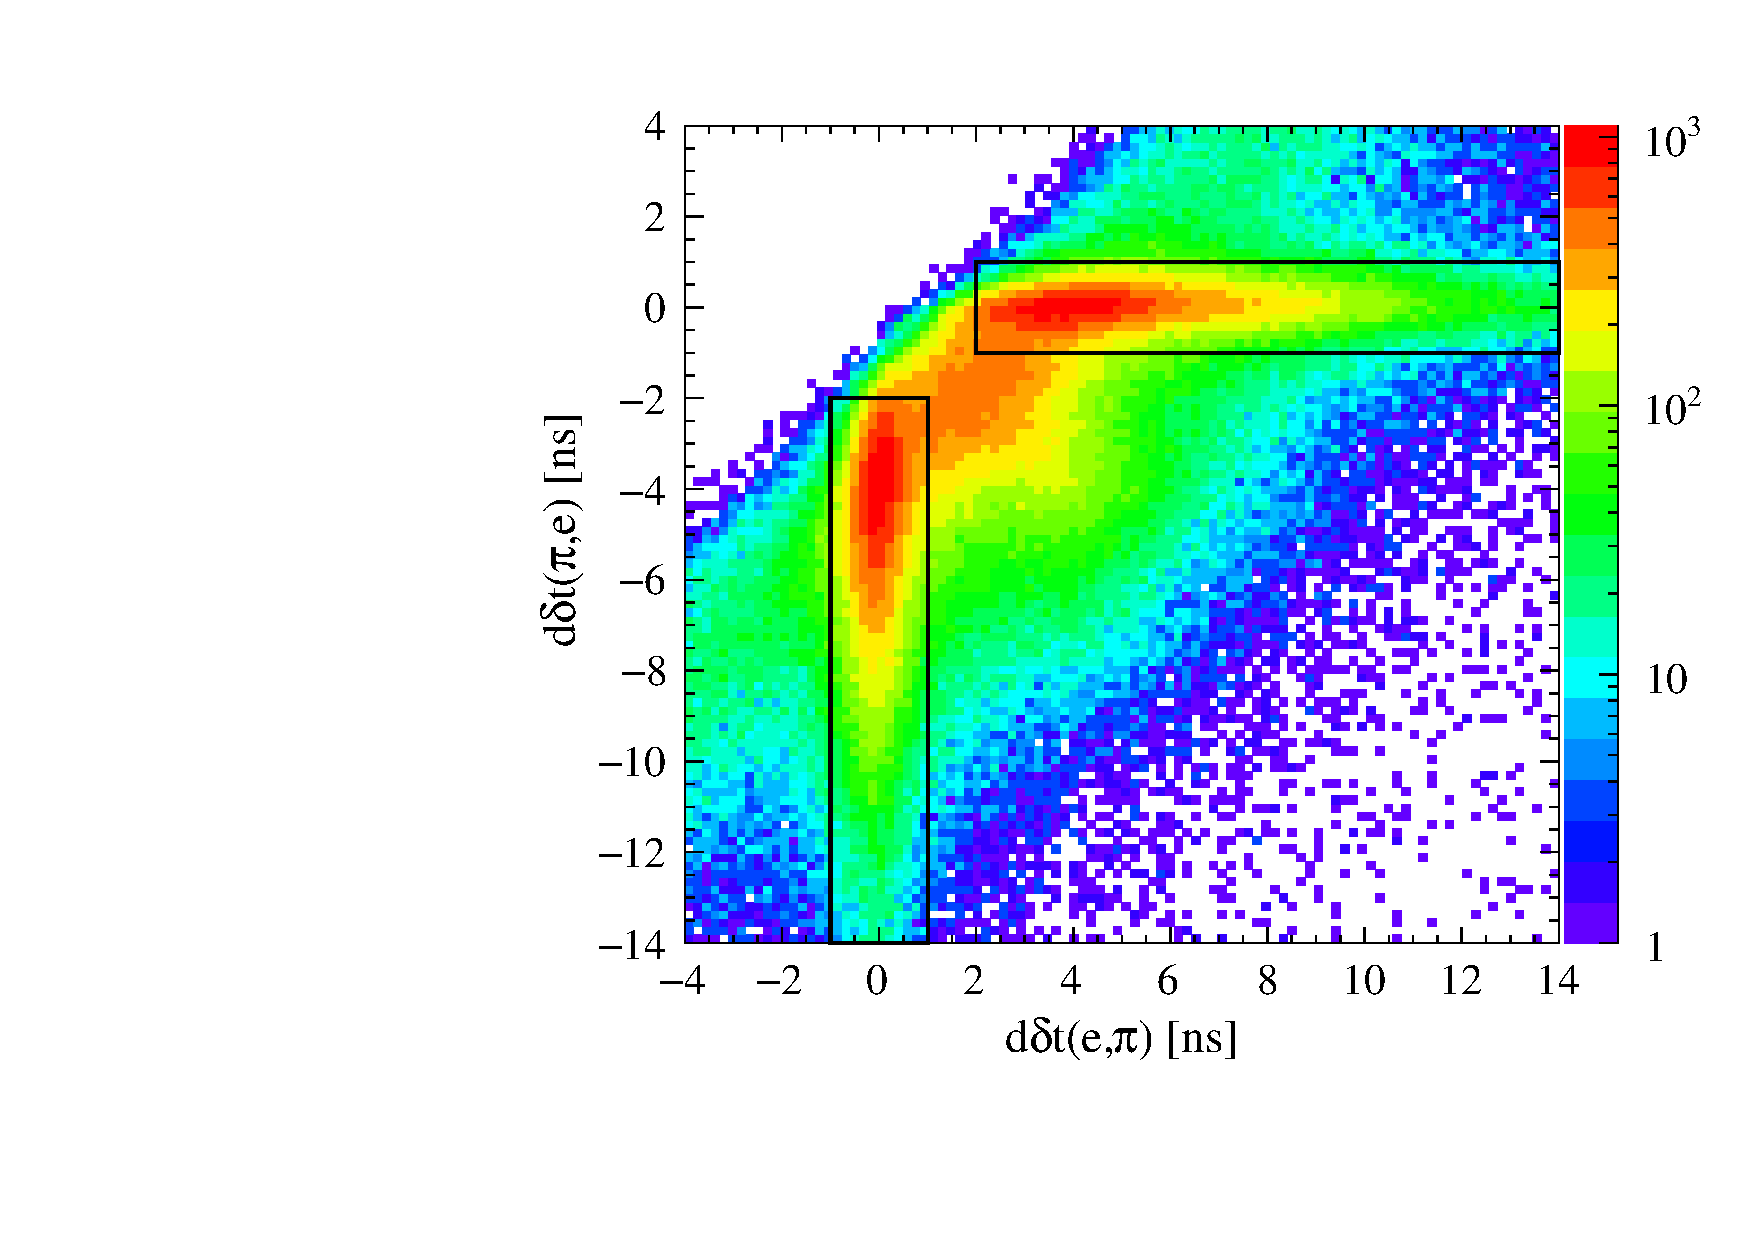
\includegraphics[width=1.0\textwidth]{Chapter7_analysis_kloe/img/t2/t2_tof1_data}
    \caption{All data events}
  \end{subfigure}  
  \caption{Errors of two possible $\pi^{\pm}$ and $e^{\mp}$ mass hypotheses assignments to tracks. Solid lines denote accepted regions, each corresponding to one of the possible mass hypotheses assignment. The MC background plot includes other $\Kl$ decays as well as combinatorial background due to incorrect choice of a DC vertex.}\label{fig:t2-tof1}
\end{figure}

Similarly as in the case of $\Ks\to\pi e \nu$, further analysis requires that each of the charged particle tracks in the decay is identified as either an electron/positron or a pion. To this end, the relative distribution of $d\delta t_{x,y} = \delta t_1(m_x) - \delta t_2(m_y),$ for two possible assignments of particle mass hypotheses to tracks was used%
\footnote{Similarly as in the case of semileptonic $\Ks$ decays, this variable is constructed so as to cancel out the event start time $T_0$. Even though the $\Kl$ decay time is also cancelled in this expression, it is retained in the definition of $\delta t(m_x)$ as later in the analysis its absolute values are used.}.
The distributions obtained with simulated $\Kl\to\pi e \nu$ events and a correct choice of the DC vertex, as well as Monte-Carlo simulated background processes and wrong vertex choices for signal events (combinatorial background), are presented in~\fref{fig:t2-tof1} along with the total spectrum obtained with KLOE data. As visible in the upper left panel, for signal events and a correctly identified $\Kl\to\pi e\nu$ decay vertex and tracks, one of the $d\delta t$ values tends to be close to zero, indicating that the assumed hypothesis on particle masses attributed to tracks was correct. A DC vertex with 2 tracks is thus considered a valid candidate if its calculated $d\delta t(e,\pi)$ and $d\delta t(\pi,e)$ values lie within one of the marked rectangular regions. 

\begin{figure}[h!]
  \captionsetup[subfigure]{justification=centering}
  \centering
  \begin{subfigure}{0.45\textwidth}
    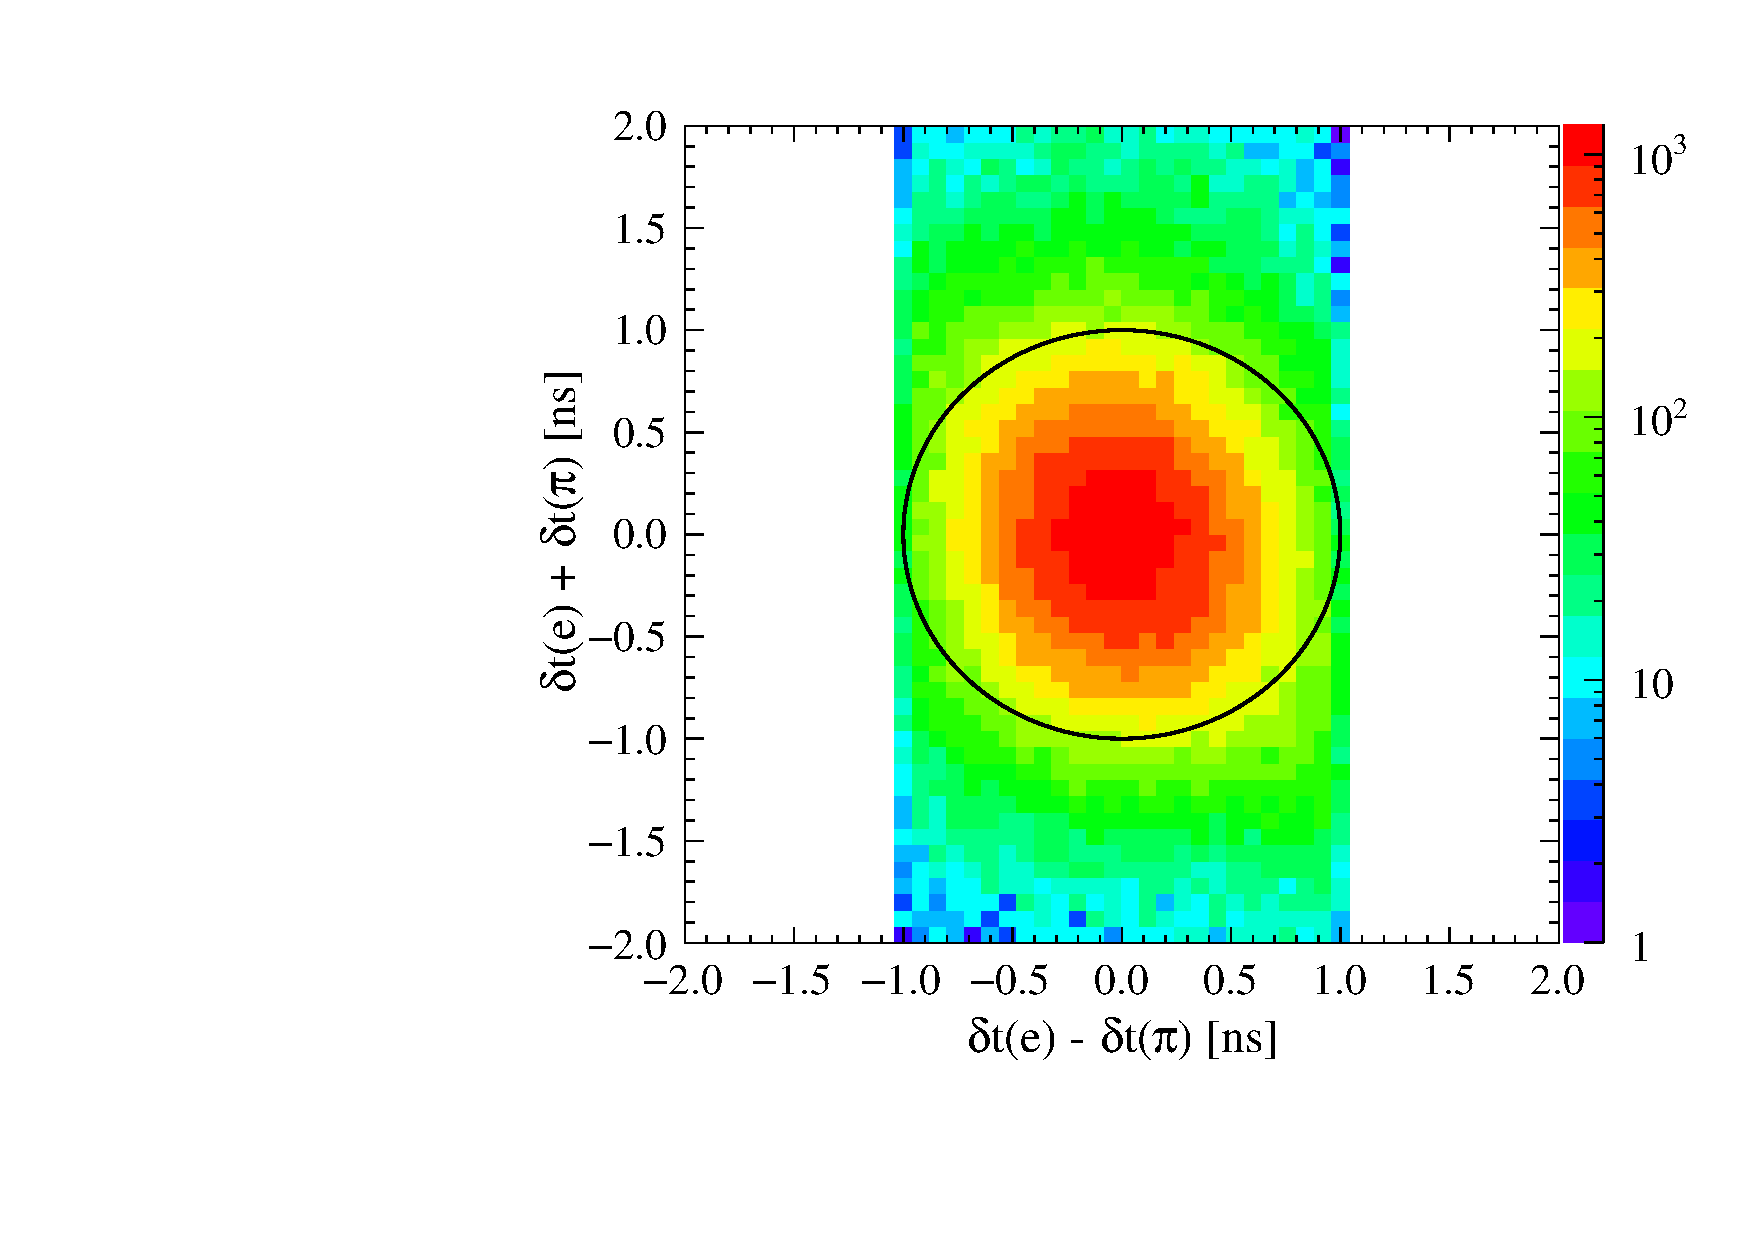
\includegraphics[width=1.0\textwidth]{Chapter7_analysis_kloe/img/t2/t2_tof2_signal}
    \caption{Signal events (MC)}
  \end{subfigure}
  %
  \begin{subfigure}{0.45\textwidth}
    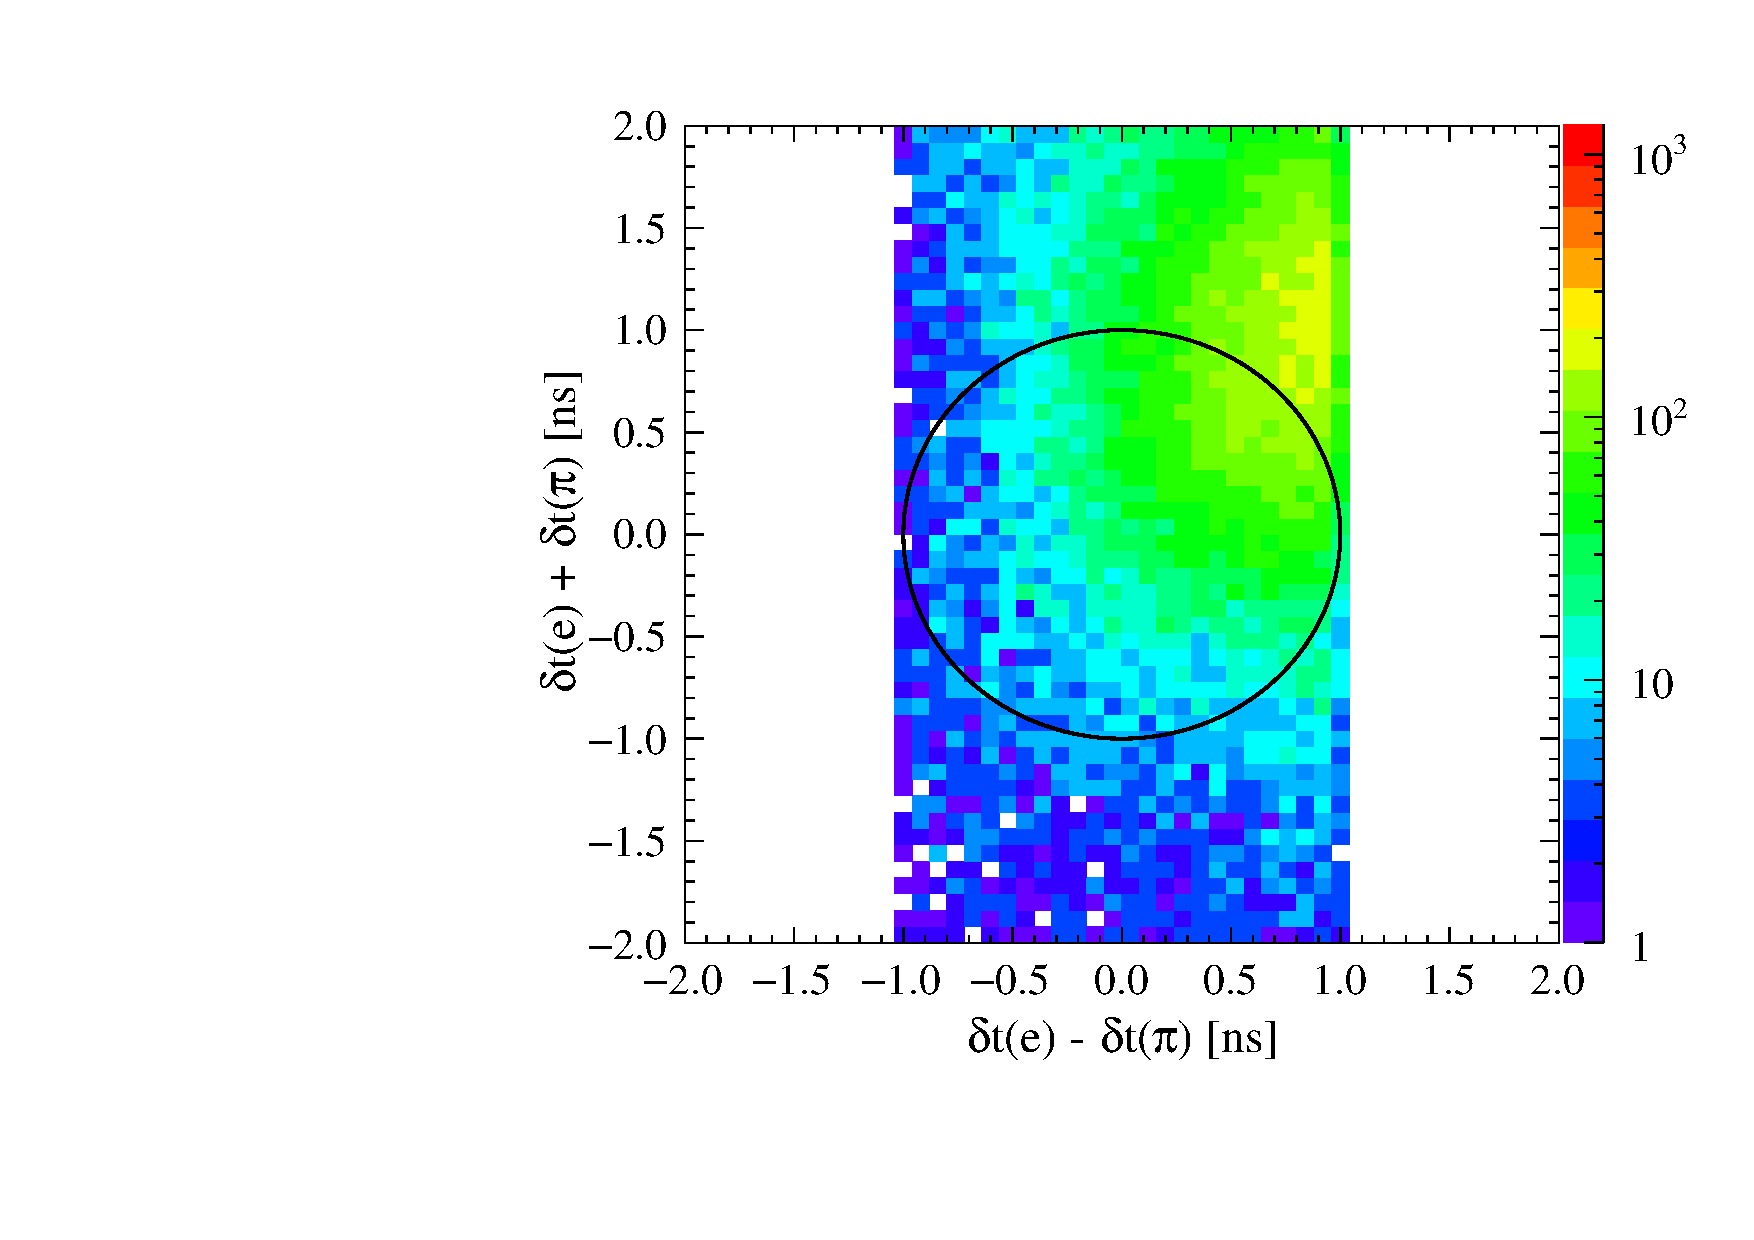
\includegraphics[width=1.0\textwidth]{Chapter7_analysis_kloe/img/t2/t2_tof2_background}
    \caption{Background events (MC)}
  \end{subfigure}
  %
  \begin{subfigure}{0.45\textwidth}
    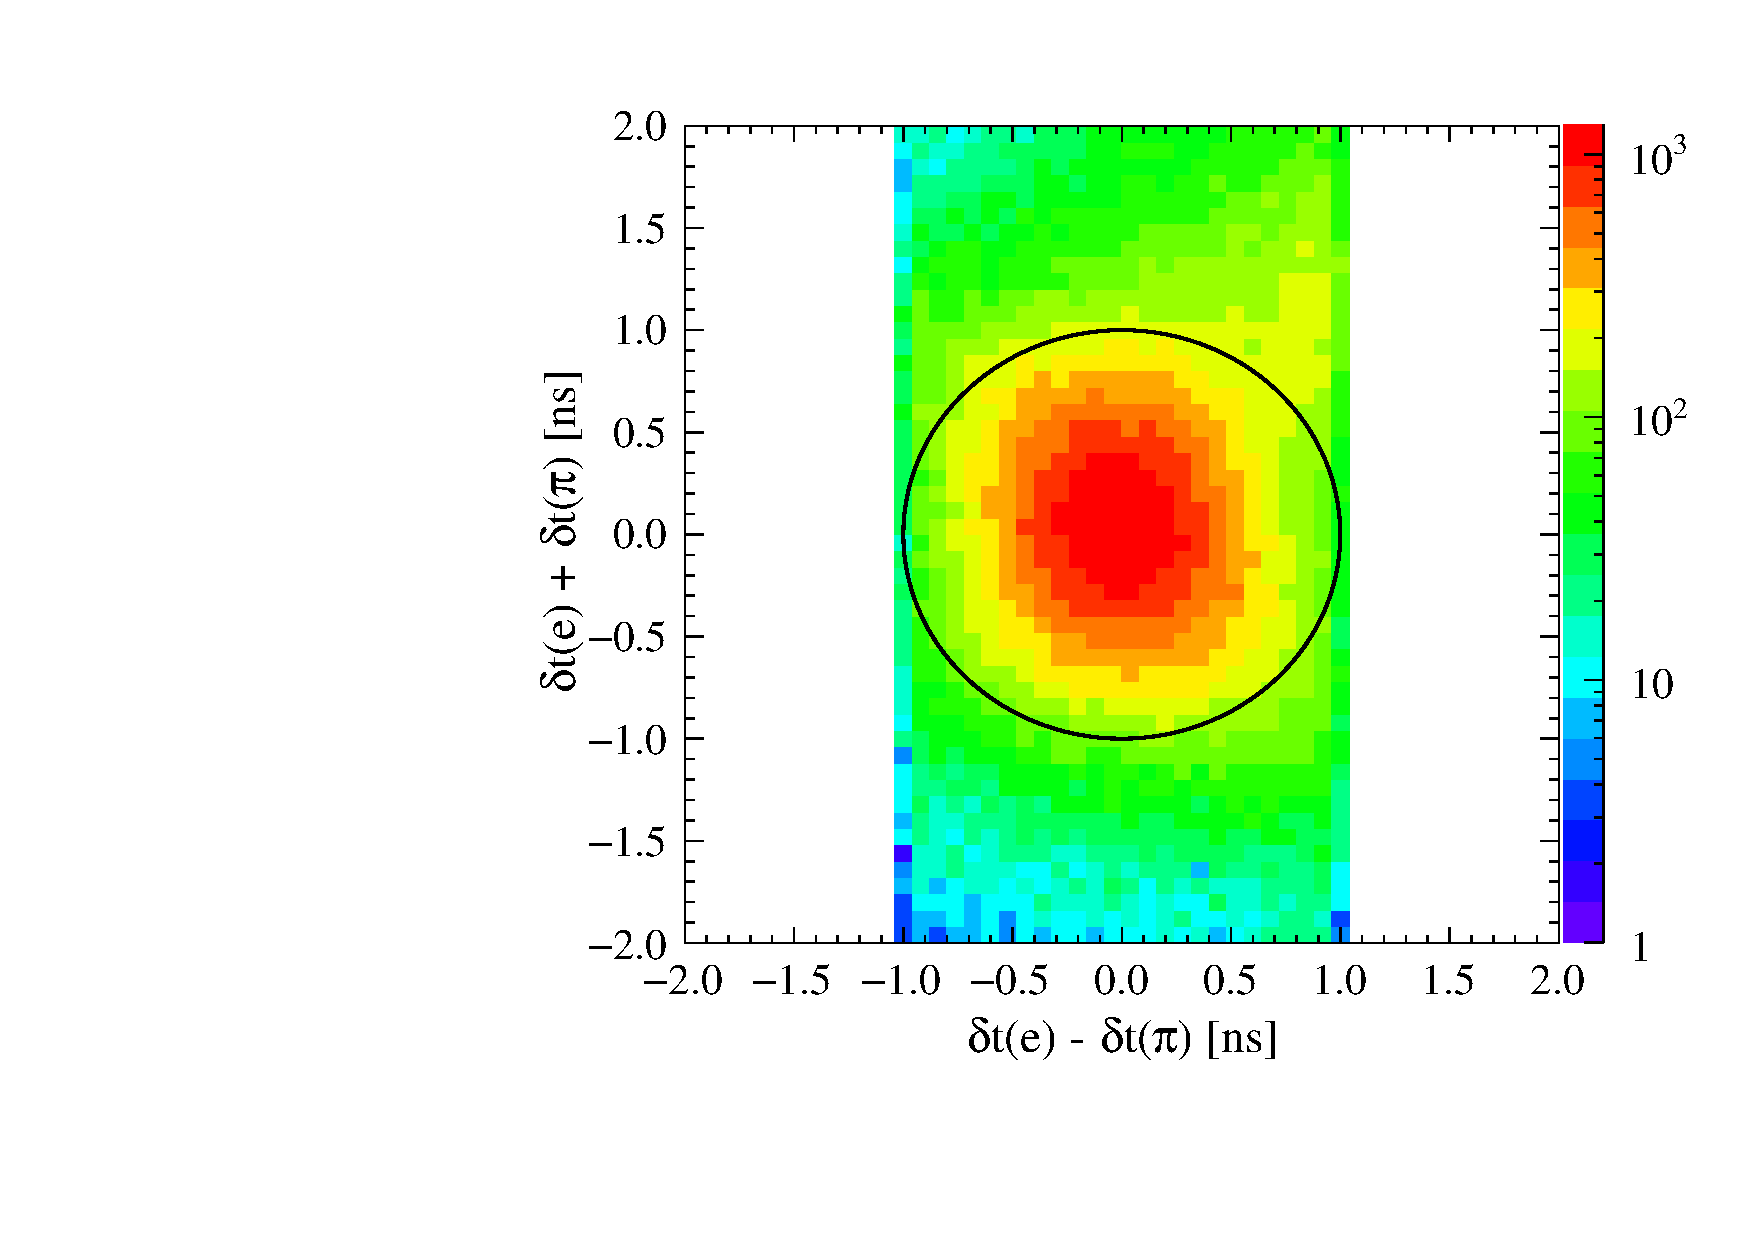
\includegraphics[width=1.0\textwidth]{Chapter7_analysis_kloe/img/t2/t2_tof2_data}
    \caption{All data events}
  \end{subfigure}  
  \caption{Relative distribution of the sum and difference of times of flight for the decay products identified as electron/positron and pion. Limits of the populated region result form the previous TOF cut (compare~\fref{fig:t2-tof1}). The MC background plot includes other $\Kl$ decays as well as combinatorial background due to incorrect choice of a DC vertex. Vertex candidates which lie outside the circle are discarded.}\label{fig:t2-tof2}
\end{figure}

Once the tracks associated with a given vertex candidate had been identified as $e^{\pm}$ and $\pi^{\pm}$, the correct discrepancies between expected and recorded time of flight $\delta t$ can be calculated for each of these particles. A relative distribution of their sum and difference is useful for discrimination of the remaining background~\cite{kloe_memo_334}. Using the distributions presented in~\fref{fig:t2-tof2} vertex candidates were selected if their respective values were located in the central region limited by a circle marked with a solid line:
\begin{equation*}
  \left(\delta t(e)-\delta t(\pi)\right)^{2} +  \left(\delta t(e)+\delta t(\pi)\right)^{2} < (0.9\:\text{ns})^2.
\end{equation*}

The green histogram in~\fref{fig:klvtxcount} shows the multiplicity of $\Kl$ decay vertex candidates per event surviving the above selection. If none of the DC vertices present in a event passed the TOF-based criteria, the event was rejected. Events with more than one remaining candidate were discarded as well to avoid further ambiguity, resulting in a loss of signal at a \SI{0.1}{\percent} level only.

Once the $\Kl\to\pi e \nu$ decay vertex and tracks of its products were identified, proper times of decay were calculated for each of the kaons in the process using their travelled path lengths and velocities as in~\eref{eq:ks_proper_time} and track curvature with respect to KLOE magnetic field was used to determine the charge of lepton in the decay.

\subsection{Requirements on the mass attributed to product tracks}
\label{sec:trackmass}
After the $\Kl$ decay vertex identification involving time of flight analysis presented in the previous Section, the signal to background ratio among the surviving events is about 13.9. The remaining background, mostly originating from $\Kl\to\pi\mu\nu$ decays, can be discriminated using quantities related to missing mass in the decay. To this end, the following variables were defined for each of the two tracks identified as $\Kl$ decay products (referred to by the particle charge):
\begin{equation}
  \label{eq:mplus_mminus}
  m^2_{\pm} = (E_K-E(\pi)_{\mp}-|\vec{p}_{miss}|)^2-\abs{\vec{p}_{\pm}}^2,
\end{equation}
where $E_K$ is the energy of the decaying kaon, $E(\pi)_{\mp}$ is the energy attributed to the track of negative (positive) charge with an assumption it was a charged pion, $\vec{p}_{\pm}$ is the momentum corresponding to positive (negative) charge track and $\vec{p}_{miss}$ is a difference between momentum of the kaon and its recorded products. As these quantities may be understood as squared masses related to each of the particle tracks in the decay, semileptonic decays with an electron or positron, whose mass is negligible compared to $\pi^{\pm}$, are characterized by $m^2_{+}$ and $m^2_{-}$ close to zero as opposed to decays with much heavier muons. Relative distributions of $m^2_{+}$ and $m^2_{-}$ displayed in~\fref{fig:t2-mmiss} reveal good separation of signal and background. To reject $\Kl\to\pi\mu\nu$, only events lying below the marked anti-diagonal line were accepted, which corresponds to the following cut on the $m^2_{+}+m^2_{-}$ sum presented in the last panel of~\fref{fig:t2-mmiss:sum}:
\begin{equation*}
m^2_{+} + m^2_{-} < 0.015\:(\text{GeV}/c^{2})^2.
\end{equation*}

\begin{figure}[h!]
  \captionsetup[subfigure]{justification=centering}
  \centering
  \begin{subfigure}{0.45\textwidth}
  \begin{tikzpicture}
    \node[anchor=south west,inner sep=0] at (0,0) 
    {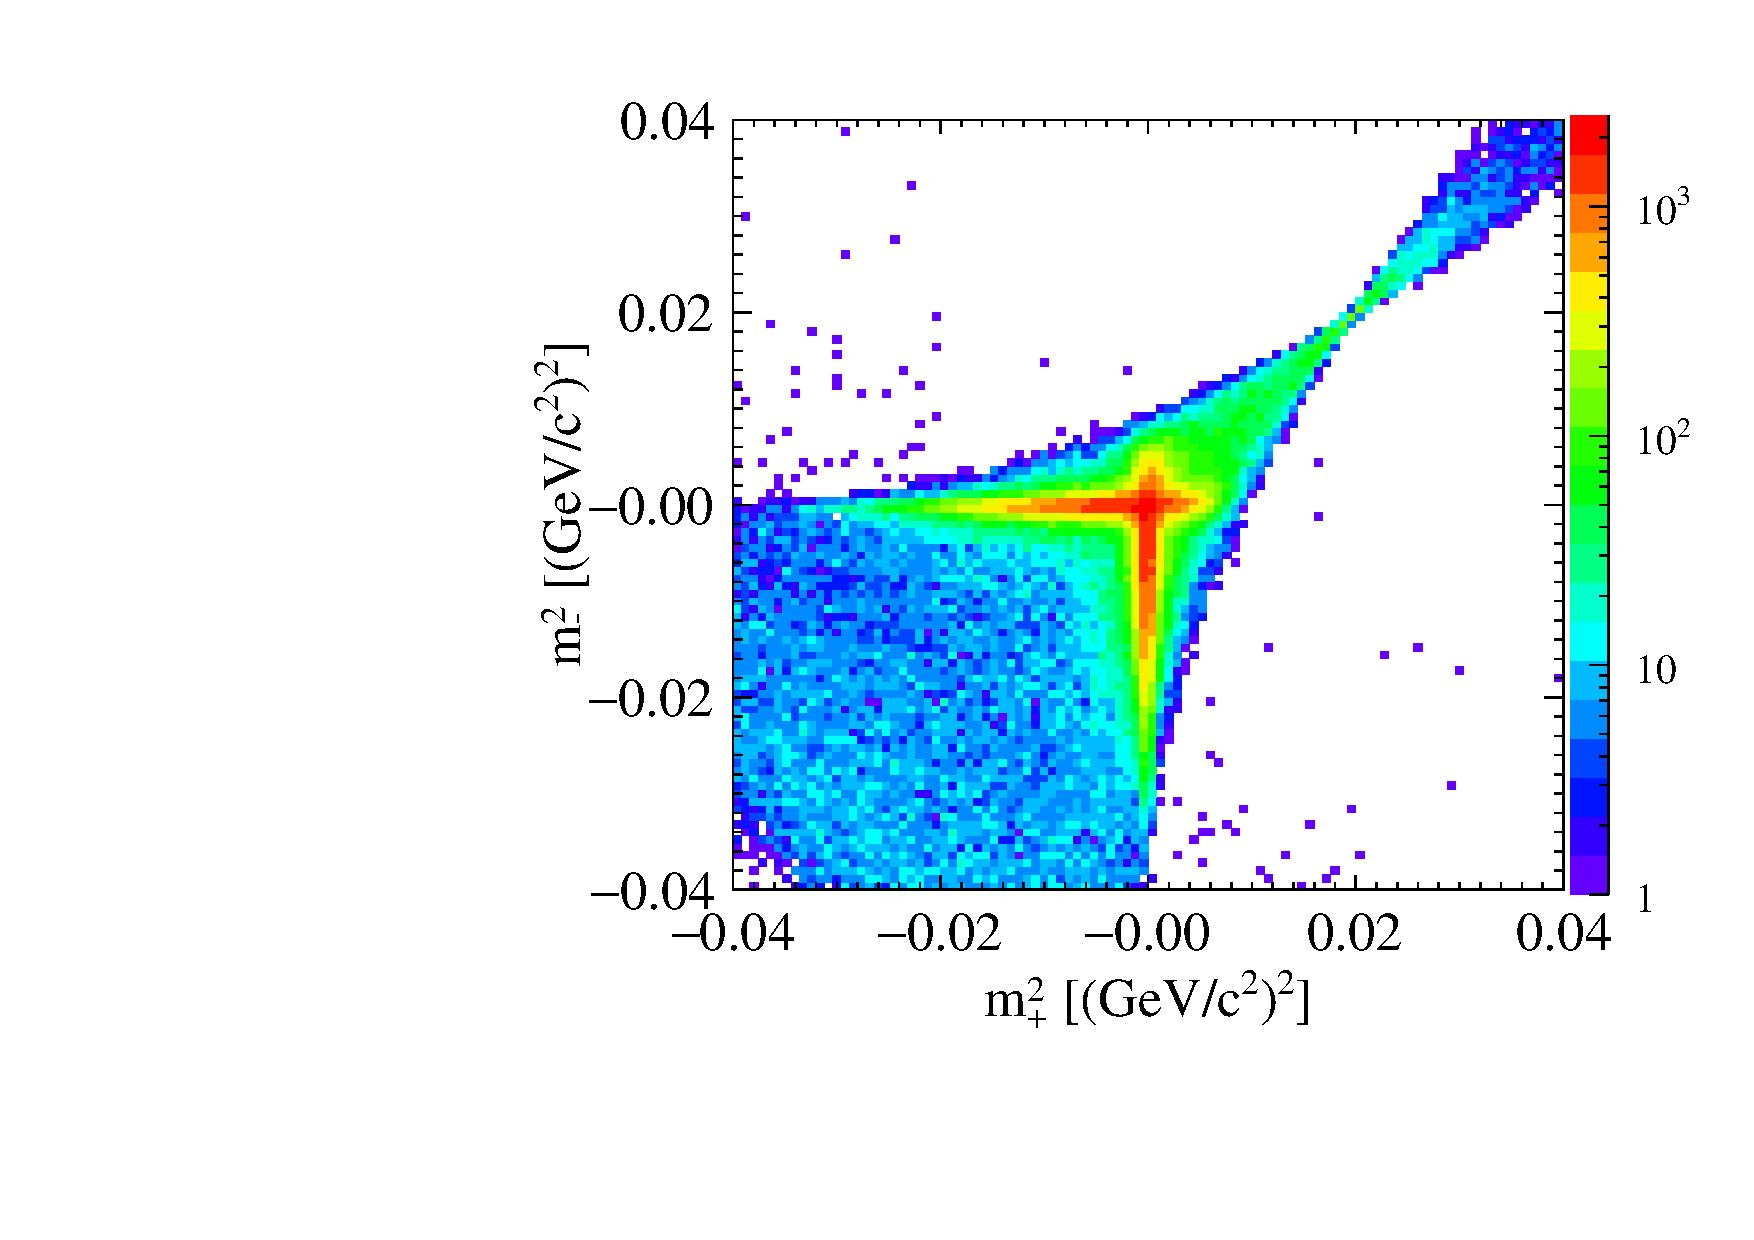
\includegraphics[width=1.0\textwidth]{Chapter7_analysis_kloe/img/t2/mmiss2_signal}};
    \draw[black, thick, dashed] (2.50,5.0) -- (5.50,2.0);
  \end{tikzpicture}
    \caption{Signal events(MC)}
  \end{subfigure}
  %
  \hspace{1em}
  \begin{subfigure}{0.45\textwidth}
  \begin{tikzpicture}
    \node[anchor=south west,inner sep=0] at (0,0) 
    {\includegraphics[width=1.0\textwidth]{Chapter7_analysis_kloe/img/t2/mmiss2_background}};
    \draw[black, thick, dashed] (2.50,5.0) -- (5.50,2.0);
  \end{tikzpicture}
    \caption{Background events (MC)}
  \end{subfigure}
  %
  \begin{subfigure}{0.45\textwidth}
  \begin{tikzpicture}
    \node[anchor=south west,inner sep=0] at (0,0) 
    {\includegraphics[width=1.0\textwidth]{Chapter7_analysis_kloe/img/t2/mmiss2_data}};
    \draw[black, thick, dashed] (2.50,5.0) -- (5.50,2.0);
  \end{tikzpicture}
    \caption{All data events}
  \end{subfigure}
  %
  \hspace{0.8em}
  \begin{subfigure}{0.45\textwidth}
    \begin{tikzpicture}
      \node[anchor=south west,inner sep=0] at (0,0) 
      {\includegraphics[width=1.0\textwidth]{Chapter7_analysis_kloe/img/t2/mmiss2_sum}};
      \draw[black, thick, dashed] (4.34,0.8) -- (4.34,4.0);
      \draw[ultra thick, black!70!white, ->] (4.32, 1.2) -- (3.7, 1.2);
    \end{tikzpicture}
    \caption{Sum of $m^2_{\pm}$, MC and data events}\label{fig:t2-mmiss:sum}
  \end{subfigure}
   % 
  \caption{Distributions of the $m^2_{+}$ and $m^2_{-}$ variables corresponding to squared masses of particles attributed to the tracks with positive and negative charge, with assumption that the other track corresponded to a charged pion. Dashed line denotes the value of a cut imposed on the sum of $m^2_{+}$ and $m^2_{-}$ whose distribution is displayed in (D).}\label{fig:t2-mmiss}
\end{figure}

The cut on $m^2_{+} + m^2_{-}$ is very powerful in terms of discrimination of background from decays other than $\Kl\to\pi e\nu$, increasing the total signal to background ratio in the selected sample of $\Ks\Kl\to\pi^+\pi^-\;\pi e\nu$ from about 14 to 64. It should be noted, however, that the same cut could not have been employed to the selection of semileptonic decays of $\Ks$ in the study of $\Ks\Kl\to\pi e\nu\;3\pi^0$ as the calculated mass values strongly depend on resolution of the input kaon momentum, which is significantly lower when obtained from the $\Kl\to 3\pi^0$ decay. After this stage of selection, the S/B ratio among the events selected as $\Ks\Kl\to\pi^+\pi^-\;\pi e\nu$ was almost twice as large as for the other class of processes, therefore no further purification of the event sample was attempted.

\section{Determination of event selection efficiencies}
\label{sec:efficiencies}

\subsection{Study of applied selection criteria performance with Monte Carlo simulations}
\label{sec:eff-mc}
Performance of each of the event selection cuts described in the previous Sections was
assessed using Monte Carlo-simulated events by evaluating the cuts' efficiency for signal events as well as signal to background ratio obtained after each cut. Results are presented in Tables~\ref{tab:eff_mc_t1} and~\ref{tab:eff_mc_t2} respectively for selection of the $\Ks\Kl\to\pi e\nu\;3\pi^0$ and $\Ks\Kl\to\pi^+\pi^-\;\pi e\nu$ processes.
In case of several cuts used to select semileptonic decays which rely on interaction of the decay products in the electromagnetic calorimeter, there is a discrepancy in the efficiency between $\pi^+e^-$ and $\pi^-e^+$. This effect is caused by different interactions allowed for positively and negatively charged pions in the EMC material, leading to a higher registration probability for $\pi^+$~\cite{Marin:1998zf}.

\begin{table}[h!]
  \centering
  \caption{Subsequent cuts and reconstruction requirements applied in the selection of $\Ks\Kl\to\pi e\nu\;3\pi^0$ events with the signal efficiencies of each step and signal to background ratio after that step. Signal is understood as events defined by both kaon decays, i.e.\ $\Ks\Kl\to\pi e\nu\;3\pi^0$. Efficiencies were obtained by applying the selection to Monte Carlo-simulated events. For the steps where efficiency differs significantly depending on the charge of lepton on the semileptonic decay, separate efficiency values were given.}\label{tab:eff_mc_t1}
  \begin{tabular}{cccc}
    \toprule
    Cut description & Section & \makecell{Cut\\efficiency [\%]} & \makecell{S/B\\after cut} \\ 
    \midrule
    \addlinespace[1ex]
    \makecell{2 DC tracks with common vertex\\
    within $r_T=<$15~cm and $|z|<$10~cm} & \ref{sec:preselection-t1} & 85.26 & 0.001 \\
    \addlinespace[1ex]
    \makecell{6 or more EMC clusters with E>20 MeV\\
    and not associated to DC tracks} & \ref{sec:preselection-t1} & 57.88 & 0.007 \\
    \addlinespace[1ex]
    \makecell{At least one 6-cluster set\\
    matching the $\Kl\to 3\pi^0\to 6\gamma$ hypothesis} & \ref{sec:kl3pi0} & 82.48 & 0.009 \\
    \addlinespace[1ex]
    \makecell{$   \ang{40} < \alpha_{CM} < \ang{170}$ and\\
    $\text{M}(\pi,\pi) < 490\:\text{MeV/c}^{2}$} & \ref{sec:ksemil} & 91.45 & 0.013\\
    \addlinespace[1ex]
    \makecell{Correct extrapolation of both\\
    DC tracks to EMC clusters} & \ref{sec:t1_tof} & 43.61 & 0.014\\
    \addlinespace[1ex]
    \makecell{TOF cuts on $|d\delta t_{\pi,\pi}| \in (1.5,\;10)\:\text{ns}$\\
    and $d\delta t_{e,\pi}$ vs $d\delta t_{\pi,e}$} & \ref{sec:t1_tof} & \makecell{89.34 ($\pi^+e^-\bar{\nu}$)\\86.33 ($\pi^-e^+\nu$)} & 0.178 \\
    \addlinespace[1ex]
    \makecell{TOF cut on $\delta t(\pi)$ vs $\delta t(e)$} & \ref{sec:t1-fine-selection} & \makecell{92.33 ($\pi^+e^-\bar{\nu}$)\\90.35 ($\pi^-e^+\nu$)} & 1.05 \\
    \addlinespace[1ex]
    \makecell{Rejection of $\Ks\to\pi^0\pi^0$ by identification\\
    of prompt photons with R/(cT)> 0.9} & \ref{sec:ks2pi0_rejection} & 95.78 & 2.7 \\
    \addlinespace[1ex]
    \makecell{Cut on $d_{PCA}$ vs $\Delta E(\pi,e)$} & \ref{sec:t1-fine-selection} & \makecell{85.93 ($\pi^+e^-\bar{\nu}$)\\86.82 ($\pi^-e^+\nu$)} & 11.3 \\
    \addlinespace[1ex]
    \makecell{$\Ks\to\pi^+\pi^-(\to\pi\mu\nu)$ rejection\\
    using $e/\pi$ and $e/\mu$ classifiers} & \ref{sec:pimu_rejection} & \makecell{94.28 ($\pi^+e^-\bar{\nu}$)\\96.31 ($\pi^-e^+\nu$)} & 33.5 \\
    \bottomrule
  \end{tabular}
\end{table}

As the observables of the \Ts~symmetry test, the $R_2^{exp}$ and $R_4^{exp}$ ratios of double decay rates will be considered as functions of the time difference between kaon decays in an event, the efficiencies used to correct the experimentally recorded decay rate spectra must be studies separately for intervals of possible $\Delta t$ values. Such $\Delta t$-dependent efficiencies were determined using MC as well as using KLOE data and independent control samples discussed in the next subsection.

\begin{table}[h!]
  \centering
  \caption{Subsequent cuts and reconstruction requirements applied in the selection of $\Ks\Kl\to\pi^+\pi^-\;\pi e\nu$ events with the signal efficiencies of each step and signal to background ratio after that step. Signal is understood as events defined by both kaon decays, i.e.\ $\Ks\Kl\to\pi^+\pi^-\;\pi e\nu$. Efficiencies were obtained by applying the selection to Monte Carlo-simulated events. For the steps where efficiency differs significantly depending on the charge of lepton on the semileptonic decay, separate efficiency values were given.}\label{tab:eff_mc_t2}
  \begin{tabular}{cccc}
    \toprule
    Cut description & Section & \makecell{Cut\\efficiency [\%]} & \makecell{S/B\\after cut} \\
    \midrule
    \makecell{2 DC tracks with common vertex\\
    within $r_T=<$15~cm and $|z|<$10~cm} & \ref{sec:kspipi} & 82.58 & 0.238 \\
    \addlinespace[1ex]
    $\abs{\text{M}(\pi,\pi) - m_{\kaon}} < 10\:\text{MeV}$ & \ref{sec:kspipi} & 86.63 & 0.276 \\
    \addlinespace[1ex]
    $\abs\Big{\abs{\vec{p}_{trk1} + \vec{p}_{trk2}} - 110\:\text{MeV/c}} < 25\:\text{MeV/c}$ & \ref{sec:kspipi} & 99.51 & 0.277 \\
    \addlinespace[1ex]
    \makecell{at least 1 set of 2 DC tracks with\\
    a common vertex excluding $\Ks\to\pi^+\pi^-$} & \ref{sec:klsemil} & 67.08 & 0.515 \\
    \addlinespace[1ex]
    \makecell{at least 1 DC vertex with correct\\
    extrapolation of 2 tracks to EMC clusters} & \ref{sec:klsemil} & \makecell{46.95 ($\pi^+e^-\bar{\nu}$)\\46.77 ($\pi^-e^+\nu$)} & 1.23 \\
    \addlinespace[1ex]
    \makecell{at least 1 DC vertex passing TOF cuts} & \ref{sec:klsemil} & \makecell{60.59 ($\pi^+e^-\bar{\nu}$)\\57.72 ($\pi^-e^+\nu$)} & 13.9 \\
    \addlinespace[1ex]
    \makecell{exactly 1 surviving $\Kl\to\pi e\nu$ vertex candidate} & \ref{sec:klsemil} & 99.89 & 14.1 \\
    \addlinespace[1ex]
    $m^2_{+} + m^2_{-} < 0.015\:(\text{GeV}/c^{2})^2$ & \ref{sec:trackmass} & 96.15 & 64.5 \\
    \bottomrule
  \end{tabular}
\end{table}

\subsection{Evaluation of selection efficiencies with KLOE data and control samples}
\label{sec:eff_data}
Total event selection efficiencies included in the final results were obtained using KLOE data
%
% TODO: add footnote about dpca exception
%
in order to avoid artifacts from possible inconsistencies between properties of MC-simulated and real events. As each of the two classes of processes studied in this analysis is constituted by two distinct neutral kaon decays, four independent control samples of events were selected from KLOE data:
\begin{itemize}
\item $\Ks\to\pi e \nu$ events where the associated $\Kl$ reached the electromagnetic calorimeter and interacted therein --- for selection efficiency of semileptonic $\Ks$ decays,
\item $\Ks\to\pi^+\pi^-$ events with a similar $\Kl$ interaction in the EMC --- for efficiency of selection of $\Ks\to\pi^+\pi^-$,
\item $\Ks\Kl\to\pi^+\pi^-\;3\pi^0$ events --- for the $\Kl\to 3\pi^0\to 6\gamma$ selection efficiency,
\item $\Ks\Kl\to\pi^0\pi^0\;\pi e\nu$ --- for selection efficiency of semileptonic decays of $\Kl$.
\end{itemize}

For each of the control samples, selection of the decay whose efficiency was under study was applied to $\phi\to\Ks\Kl$ events in the same form as selection of the main processes of interest, $\pi e\nu\;3\pi^0$ and $\pi^+\pi^-\;\pi e\nu$. Events with neutral K mesons were identified (tagged) by presence of a certain type of interaction of the kaon accompanying the one whose selection was tested. Number of the registered interactions tagging $\phi\to\Ks\Kl$ ($N_{tag}$) was multiplied by the branching ratio for the investigated kaon decay $\mathrm{K}\to\mathrm{X}$ to obtain the number of expected events:
\begin{equation}
  \label{eq:eff_n_expected_ks}
  N_{exp}^{\mathrm{K}\to\mathrm{X}} = N_{tag}\cdot \text{BR}(\mathrm{K}\to\mathrm{X}),
\end{equation}
for the case of efficiency for decays of $\Ks$, which is not limited by detector size. For estimation of the $\Kl$ decays' detection efficiency, the differential number of expected events was determined:
\begin{equation}
  \label{eq:eff_n_expected_kl}
  \frac{dN_{exp}^{\mathrm{K}\to\mathrm{X}}}{d t_{k}} = N_{tag}\cdot \text{BR}(\mathrm{K}\to\mathrm{X}) \frac{1}{\tau_L}e^{-t_K/\tau_{L}},
\end{equation}
where $t_K$ is the time of the long-lived kaon decay and $\tau_{L}$ denotes its mean lifetime.

In case of the study of early kaon decays, i.e.\ $\Ks\to\pi e\nu$ and $\Ks\to\pi^+\pi^-$, their selection efficiency was estimated as a single value independent of the kaon decay time:
\begin{equation}
  \label{eq:eff_scalar_efficiency}
  \varepsilon^{\mathrm{K}\to\mathrm{X}} = \frac{N^{\mathrm{K}\to\mathrm{X}}_{obs}}{N^{\mathrm{K}\to\mathrm{X}}_{exp}},
\end{equation}
where $N^{\mathrm{K}\to\mathrm{X}}_{obs}$ is the number of observed events, i.e.\ number of events which passed the selection under study. Uncertainty of the efficiency was evaluated using the binomial approach~\cite{behnke, statisctical_methods}:
\begin{equation}
  \label{eq:eff_binomial_error}
  \sigma\left({\varepsilon^{\mathrm{K}\to\mathrm{X}}}\right) = \frac{\sqrt{N^{\mathrm{K}\to\mathrm{X}}\left(1-\varepsilon^{\mathrm{K}\to\mathrm{X}}\right)}}{N^{\mathrm{K}\to\mathrm{X}}_{exp}}.
\end{equation}

For the two late kaon decays, $\Kl\to 3\pi^0$ and  $\Kl\to\pi e\nu$, selection efficiency may depend on the location of decay inside the detector and was therefore studied separately in subsequent intervals of the proper time of kaon decay $t'_{\Kl}$. To this end, an expected $\Kl$ decay time distribution was obtained by scaling a binned exponential decay $\exp\left(-t/\tau_L\right)$ so that its integral for $t\in[0;\infty)$ was equal to the expected number of events obtained as shown in~\eref{eq:eff_n_expected_kl}. For events surviving the selection whose efficiency was investigated, the observed $t'_{\Kl}$ spectrum was obtained with the same binning as the expected exponential decay. Finally, the efficiency was evaluated for each $t'_{\Kl}$ interval as a ratio of observed to expected counts in a given bin of the $t'_{\Kl}$ distributions. Uncertainty of efficiency in each bin was again calculated assuming binomial errors as in~\eref{eq:eff_binomial_error}. Efficiencies of selection of the semileptonic decays were determined separately for each of the two lepton charges.

Total efficiencies of selection of the two main classes of studied processes, $\pi e\nu\;3\pi^0$ and $\pi^+\pi^-\;\pi e\nu$, which are required for further analysis, must be expressed as functions of the difference of kaons' proper decay times. As the aforementioned efficiency estimation scheme results in independent values for each of the kaon decays, total efficiencies for double kaon decay events were calculated with the following approximations for the two processes of interest:
\begin{equation*}
%  \label{eq:eff_approximation}
  \begin{split}
    \Delta t & = t_{3\pi^{0}} - t_{\pi e \nu} \\
             & \approx\ t_{3\pi^{0}} \text{\ \ for\ \ }{t_{3\pi^{0}} \gg t_{\pi e \nu}},  \\  
   \Delta t & = t_{\pi e \nu} - t_{\pi^+\pi^-} \\
            & \approx\ t_{\pi e \nu} \text{\ \ for\ \ } {t_{\pi e \nu} \gg t_{\pi^+\pi^-}},
          \end{split}
\end{equation*}
valid for $\Delta t\gg 0$, which is sufficient to obtain a correct efficiency estimate for the asymptotic region of the double kaon decay rates. Consequently, the efficiency for large time differences was obtained from the time-dependent efficiency distributions for the late kaon decays, uniformly scaled with the single-value efficiencies for the early kaon decays.

\subsection{The $\Ks\to\pi e\nu$ and $\Ks\to\pi^+\pi^-$ control samples}
In the two control samples used for evaluation of efficiency for $\Ks\to\pi e\nu$ and $\Ks\to\pi^+\pi^-$, presence of neutral kaons in an event was identified by requiring that an interaction of the long-lived neutral meson was recorded in the EMC. As this happens for about \SI{60}{\percent} of $\phi\to\Ks\Kl$ decays, a clean sample of neutral kaon pairs is obtained this way.
Identification of $\Kl$ interactions in the calorimeter was based on the procedure described in References~\cite{daria_article, daria_memo, silarski_phd}.
Such events are characterized by a large energy deposit not related to any drift chamber track, therefore all clusters without track association and $E>100$~MeV were considered as $\Kl$ interaction candidates. Moreover, due to the p-wave distribution of polar angles $\theta$ of kaons' emission in a $\phi$ decay, given by:
\begin{equation}
  \label{eq:pwave}
  \frac{dN}{d\Omega} \propto \sin^2\theta,
\end{equation}
a majority of the $\Kl$ reaching the calorimeter are expected to interact in the barrel part. EMC clusters located in the end-caps are thus excluded to discriminate machine background. As in the analysis of $\Kl\to 3\pi^0$ the momentum direction of the long-lived kaon is not restricted (not to compromise selection efficiency), Monte Carlo simulations were used to confirm that the efficiency for selection of $\Ks$ decays does not exhibit a significant dependence on the momentum direction of the associated $\Kl$.

%
% MEMO TODO: dodać stosowny obrazek z rozkładem kątowym i liczby dowodzące, że to nie ma znaczenia
%
As the average velocity of a kaon produced in a $\phi$ decay at DA$\Phi$NE is well defined and amounts to about $\beta\approx 0.22$, the hypothetical $\Kl$ velocity was calculated for each candidate cluster as $\beta_{cl} = \frac{R_{cl}}{cT_{cl}}$ where $R_{cl}$ denotes distance between average $\phi$ decay point and the EMC cluster recorded at time $T_{cl}$ and $c$ is the speed of light (see~\sref{sec:ks2pi0_rejection} where a similar variable is used to identify clusters from prompt photons). The $\beta_{cl}$ value was transformed to the CM reference frame of $\phi$ and restricted to the region:
\begin{equation}
  \label{eq:betacl}
   0.2 < \beta^{CM(\phi)}_{cl} < 0.25,
\end{equation}
%
% MEMO TODO: dodac wykresy energii i bety
%
whose upper limit takes into account a possible shift due to incorrect $T_0$ in an event. To achieve a high sample purity, the selected events were finally limited to ones where the energy deposited in the EMC cluster was above 250~MeV. Tests with MC revealed that background contamination of the selected $\phi\to\Ks\Kl$ samples was about \SI{0.8}{\percent}. 

The vector spanning between average $\phi$ decay point at KLOE and location of the EMC cluster corresponding to $\Kl$ interaction provides a precise estimate of the kaon momentum direction due to large distance from detector center to the calorimeter. Momentum of the $\Ks$ meson, inferred using momentum conservation in the $\phi\to\Ks\Kl$ and $\vec{p}_{\Kl}$ direction as described in~\sref{sec:ks_from_kl} is therefore characterized by a considerably higher resolution compared to the one obtained with $\Kl\to 3\pi^{0}$. Consequently, as several steps of $\Ks\to\pi e \nu$ event selection rely on $\Ks$ momentum estimate obtained from the partner kaon, the total selection performance is prone to behave differently when applied to the control sample rather than to $\Kl\to 3\pi^{0}$ events. Therefore, the $\vec{p}_{\Kl}$ direction obtained using the respective EMC cluster location in case of the control sample was subjected to an artificial smearing with double Gaussian resolution model obtained with Monte Carlo-simulated $\Ks\Kl\to 3\pi^0\;\pi e\nu$ events. In case of the other control sample, $\Ks\to\pi^+\pi^-$, the event selection does not use the momentum estimate from $\Kl$ and therefore no smearing was introduced.
%
% MEMO TODO: Dokładny opis i wykresy do smearingu
%

\subsection{The $\Ks\Kl\to\pi^+\pi^-\;3\pi^0$ and $\Ks\Kl\to\pi^0\pi^0\;\pi e\nu$ control samples}
For estimation of the $\Kl\to 3\pi^0$ selection efficiency, these decays were tagged by a $\Ks$ decaying into charged pions. The applied selection of $\Ks\to\pi^+\pi^-$ was based on the already devised cuts discussed in~\sref{sec:kspipi}, which allow for preparation of a $\phi\to\Ks\Kl$ sample with a background contamination at a level below \SI{1}{\percent}. As the studied selection of $\Kl$ decays into neutral pions does not use any information related to the $\Ks$ decay, it was applied to the selected sample without further preparations.

In the control sample used to determine the selection efficiency of semileptonic decays of the long-lived neutral kaon, $\phi\to\Ks\Kl$ events were tagged by the $\Ks\to\pi^0\pi^0$ decay. Selection of neutral hadronic decays of Ks was performed following the approach described in Reference~\cite{memo_225}. Firstly, presence of at least 3 EMC clusters was required whose total energy was above 300~MeV. Each of the clusters matching these requirements was required to have a deposited energy in the range $(20;300)$~MeV and a polar angle above 21$^\circ$ to differentiate them from machine background. Subsequently, the clusters were required to match a prompt photon hypothesis, i.e.\ $0.9<\frac{R_{cl}}{cT_{cl}}<1.2$ (compare~\sref{sec:ks2pi0_rejection}). If 4 of 5 EMC clusters satisfying the aforementioned criteria were found in an event, with a total invariant mass of the photons within the range (390; 600)~MeV and at least one of the clusters recorded in the calorimeter barrel, the event was considered a $\Ks\to\pi^0\pi^0$ candidate. Additionally, a $\Ks\to\pi^+\pi^-$ veto was applied by negation of the selection conditions described in~\sref{sec:kspipi}.
According to MC-based studies, purity of the selected $\Ks\to\pi^0\pi^0$ event sample was at the level of \SI{98}{\percent}. Although the $\Ks$ momentum estimate available from photons' momenta in the $\Ks\to\pi^0\pi^0$ is considerably worse than in case of the charged pion channel, the selection of $\Kl\to\pi e\nu$ decays was prepared so as to be independent of accompanying kaon decay and its properties, and thus the tested cuts were applied directly to the control sample.

\subsection{MC-based correction to $\pi e\nu\;3\pi^0$ efficiency obtained with data}\label{sec:dpca_correction}
The scheme of determination of efficiencies based on independent control samples for each of the kaon decays relies on an assumption that the efficiency for $\Ks$ decay selection does not depend on the time of decay of $\Kl$ in the same event, so that it may be approximated by a single number uniformly scaling the $t_{\Kl}$-based efficiency for the associated $\Kl$ decay. It was tested with Monte Carlo simulations that this assumption is valid for all of the analysis steps except for the cut on $d_{PCA}$ vs. $\Delta E(\pi,e)$ described in~\sref{sec:t1-fine-selection}. In case of this cut, the $\Delta E(\pi,e)$ value is calculated using i.a.\ the total momentum of the decaying $\Ks$ meson. As the latter is inferred indirectly from the $\phi$ decay kinematics and $\Kl$ momentum direction, this variable is sensitive to the angular resolution of estimated $\Kl$ flight direction. Although the spatial resolution for $\Kl\to 3\pi^0$ is mostly constant (see~\fref{fig:t2-kspipi}, left), decays, the angular resolution of $\Kl$ direction varies strongly with decay distance from the primary interaction point, influencing $\vec{p}_{\Ks}$ resolution as visible in~\fref{fig:ks_angle_resolution}. Consequently, the shape of efficiency of the $d_{PCA}$ vs. $\Delta E(\pi,e)$ cut as a function of $\Delta t$ is not uniform as in~\fref{fig:dpca_eff_mc}. However, this selection step is powerful in terms of background rejection (see~\tref{tab:eff_mc_t1}) and thus cannot be removed from the analysis chain. Whereas it could be replaced by constraints imposed on other kinematical quantities sensitive to the $\Ks\to\pi^+\pi^-(\to\pi\mu\nu)$ background such as missing mass, the same effect is still expected as such variables also depend on accuracy of the $\Ks$ momentum estimation.
\begin{figure}[h!]
  \centering
  \includegraphics[width=0.7\textwidth]{Chapter7_analysis_kloe/img/common/dpca_de_eff}
  \caption{Shape of the $d_{PCA}$ vs. $\Delta E(\pi,e)$ cut efficiency as a function of kaons' decay time difference based on Monte Carlo-simulated $\pi e\nu\;3\pi^{0}$ events.}\label{fig:dpca_eff_mc}
\end{figure}

As shape of this efficiency cannot be reproduced using independent control samples for $\Ks\to\pi e\nu$ and $\Kl\to 3\pi^0$, the efficiency for selection of $\Ks$ semileptonic decays was estimated using control data sample and applying all selection steps except the requirement on $d_{PCA}$ vs. $\Delta E(\pi,e)$. Subsequently, a Monte Carlo simulation-based correction for the efficiency of this cut presented in~\fref{fig:dpca_eff_mc} was imposed on the data-derived efficiencies to obtain the total efficiencies used in the determination of the final result.

\subsection{Comparison of selection efficiencies from data and MC}
\label{sec:eff_comparison}
The event selection steps described in Sections~\ref{sec:t-analysis-1} and~\ref{sec:t-analysis-2} resulted in four sets of events, each characterized by a certain pair of time-ordered neutral kaon decays:
\begin{itemize}
\item $\Ks\Kl\to\pi^+ e^- \bar{\nu}\;3\pi^{0}$,
\item $\Ks\Kl\to\pi^- e^+ {\nu}\;3\pi^{0}$,
\item $\Ks\Kl\to\pi^+\pi^-\;\pi^+ e^- \bar{\nu}$,
\item $\Ks\Kl\to\pi^+\pi^-\;\pi^- e^+ {\nu}$.
\end{itemize}

Each of the four subsamples listed above is characterized by a separate $\Delta t$-dependent event selection efficiency. Such efficiencies obtained from data and control samples as described in the previous Section are presented as black points in~\fref{fig:eff_comparison}. Efficiencies obtained using MC-generated events are shown in red points for a comparison. In each of these efficiencies, a discrepancy between data and MC-derived distributions is visible for low time differences of approximately $\Delta t < 50 \tau_{S}$, caused by the nature of the employed method of efficiency estimation using independent control samples for $\Ks$ and $\Kl$ decays. However, as the final estimation of the \Ts-asymmetric observables is concentrated on the asymptotic $\Delta t \gg \tau_{S}$ region, the further considerations are limited to $\Delta t$ ranges above this discrepancy.

\begin{figure}[h!]
  \centering
  \includegraphics[width=0.9\textwidth]{Chapter7_analysis_kloe/img/common/efficiencies_t1}  
  \includegraphics[width=0.9\textwidth]{Chapter7_analysis_kloe/img/common/efficiencies_t2}  
  \caption{Efficiencies of event selection as functions of the kaons' proper decay time difference for the four event subsamples used in the analysis. Efficiency obtained using data and an independent control sample for each kaon decay (black), used further in the determination of $R_2$ and $R_4$, is compared with efficiency obtained with generated Monte Carlo events (red). The discrepancy in the region of about $\Delta t < 50\ \tau_{S} $ visible for all subsamples is an artifact of the efficiency estimation method with control samples.}\label{fig:eff_comparison}
\end{figure}

Whereas data and MC-derived efficiencies for the $\pi^+\pi^-\;\pi e\nu$ process and large decay time differences exhibit good agreement, the efficiency for $\pi e \nu\;3\pi^0$ is overestimated in the Monte Carlo simulations, especially in terms of the excess of recorded $\pi^+e^-\bar{\nu}$ events due to different interactions of $\pi^+$ and $\pi^-$ in the KLOE calorimeter, which is less pronounced in data. This discrepancy, demonstrated in~\fref{fig:eff_comparison} is the major reason for which the efficiencies used in the determination of the final $R_2(\Delta t)$ and $R_2(\Delta t)$ distributions are based on data and control samples rather than MC simulations.

\section{Determination of probability asymmetry distributions for the T test with KLOE}\label{sec:ratios}
In order to evaluate the desired observables of the \Ts~symmetry test, i.e.\ the following ratios $\Delta t$-dependent double decay rates:
\begin{eqnarray}
  \label{eq:final_r2_and_r4}
  R_2(\Delta t) &= \frac{\mathrm{I}(\pi^+e^-\bar{\nu},3\pi^0;\Delta t)}{\mathrm{I}(\pi^+\pi^-,\pi^-e^+\nu;\Delta t)} \cdot \frac{1}{D},\\
  {R_4(\Delta t)} & = \frac{\mathrm{I}(\pi^-e^+\nu,3\pi^0;\Delta t)}{\mathrm{I}(\pi^+\pi^-,\pi^+e^-\bar{\nu};\Delta t)}  \cdot \frac{1}{D},
\end{eqnarray}
where $D$ is the constant factor discussed in~\sref{sec:d_determination}, each of the event samples listed above, along with their selection efficiencies, was divided into $\Delta t$ intervals (bins) of 3~$\tau_{S}$ width.
\fref{fig:dt_plots} presents the resulting double decay rate distributions for each of the four processes. The $R_2(\Delta t)$ and $R_4(\Delta t)$ ratios were calculated for each $i$-th bin of $\Delta t$ using the event counts in the respective distributions (referred to as $N(f_1,\:f_2;\Delta t_i)$ for final states $f_1$ and $f_2$), including selection efficiencies obtained with control data samples and the $D$ factor:
\begin{eqnarray}
  \label{eq:r2_and_r4_bin_value}
  R_{2}(\Delta t_i) &= \frac{N(\pi^+ e^-\bar{\nu},\:3\pi^0;\:\Delta t_i) / \varepsilon(\pi^+ e^-\bar{\nu},\:3\pi^0;\:\Delta t_i)}{N(\pi^+\pi^-,\:\pi^-e^+\nu;\:\Delta t_i) / \varepsilon(\pi^+\pi^-,\:\pi^-e^+\nu;\:\Delta t_i)}  \cdot \frac{1}{D},\\
  R_{4}(\Delta t_i) &= \frac{N(\pi^- e^+{\nu},\:3\pi^0;\:\Delta t_i) / \varepsilon(\pi^- e^+{\nu},\:3\pi^0;\:\Delta t_i)}{N(\pi^+\pi^-,\:\pi^+e^-\bar{\nu};\:\Delta t_i) / \varepsilon(\pi^+\pi^-,\:\pi^+ e^-\bar{\nu};\:\Delta t_i)}  \cdot \frac{1}{D}.
\end{eqnarray}

\begin{figure}[h!]
  \centering
  \includegraphics[width=0.9\textwidth]{Chapter7_analysis_kloe/img/common/dtplots}
  \caption{Double kaon decay rates as a function of the difference of kaon proper decay times for each of the studied class of events, as obtained after event selection and reconstruction. Presented distributions are not corrected for selection efficiencies. Errors on the number of counts in each bin of the histograms are Poissonian.}
  \label{fig:dt_plots}
\end{figure}

The \Ts-violation-sensitive ratios obtained in the manner described above are displayed in~\fref{fig:final_ratios}. Although for the test of symmetry under reversal in time pursued in this work only the region of kaon decay time differences significantly larger than $\Ks$ lifetime is relevant (see~\sref{sec:strategies}), the whole $\Delta t$ range available at KLOE is shown for completeness. Is should be noted, however, that in the region of small $\Delta t$ arising from comparable decay times of $\Ks$ and $\Kl$,
the assumed scheme of efficiency estimation with independent control samples for both kaons may not reproduce the true efficiency correctly. 
%the applied corrections for selection efficiencies do not reproduce the efficiency correctly
Moreover, a discrepancy between the efficiency based on data and Monte Carlo simulations revealed in~\fref{fig:eff_comparison} requires a further careful investigation and therefore for the determination of the asymptotic values of $R_2$ and $R_4$ in this work the region of $\Delta t$ below 60~$\tau_S$ was discarded.

%(compare) and thus this region may not be used to determine 
On the other hand, the region of $\Delta t$ above about 250~$\tau_S$ corresponds to $\Kl$ decays close to outer limits of the KLOE detector where limited acceptance reduces selection efficiencies leading to large statistical uncertainties on the event counts used to calculate the ratios.
%
% TODO: update based on the final efficiency distributions
%

\begin{figure}[h!]
  \centering
  \includegraphics[width=0.9\textwidth]{Chapter7_analysis_kloe/img/common/r2}\\
  \includegraphics[width=0.9\textwidth]{Chapter7_analysis_kloe/img/common/r4}
  \caption{Two ratios of double decay rates sensitive to $\Ts$ symmetry violation obtained in the analysis of KLOE experiment data presented in this Thesis. The red line presents results of maximum likelihood fits of a constant level to the ratios in the $\Delta t \gg \tau_{S}$ region.}
  \label{fig:final_ratios}
\end{figure}

In order to quantify the deviations from unity of the asymptotic levels of $R_2(\Delta t \gg \tau_S)$ and $R_4(\Delta t \gg \tau_S)$, constant values were fitted to the ratios in the following range, characterized by relatively high and stable event selection efficiencies and their agreement between control samples and MC simulations:
\begin{equation}
  \label{eq:fit_range}
  60\:\tau_S < \Delta t < 250\:\tau_S.
  %
  % TODO: update if necessary!!!
  % 
\end{equation}
Impact of the choice of upper and lower $\Delta t$ limit used for estimation of the ratios' level was incorporated into systematic uncertainty of the result. To properly account for the nature of uncertainties on the $R_2$ and $R_4$ points, the constant level calculation was performed with a dedicated binned maximum likelihood fit described in the next Section.

\subsection{Fit of the asymptotic level of double decay rates}
\label{sec:ml_fit}
Each point in the graphs of the $R_2(\Delta t)$ and $R_4(\Delta t)$ ratios shown in~\fref{fig:final_ratios} results from a division of two counts of events characterized by their $\Delta t$ value lying in a certain interval (compare~\eref{eq:r2_and_r4_bin_value}). This may be generally expressed for the $i$-th time difference interval as:
\begin{equation}
  \label{eq:fit_general_rpoint}
\forall_i:  R_i \equiv R(\Delta t_i) = \frac{N_i}{N_i'}\frac{\varepsilon_i'}{\varepsilon_i} \frac{1}{D},
\end{equation}
where $\varepsilon_i$ and $\varepsilon_i'$ are the selection efficiencies for the events counted as $N_i$ and $N_i'$ respectively.
Each of the event counts $N_i$ and $N_i'$  may be assumed to come from a Poissonian distribution with unknown mean. Although the values of $R$ depend also on the selection efficiencies and the $D$ factor, their uncertainties are negligible compared to the Poissonian errors on the event counts for the process involving the relatively rare semileptonic decays of $\Ks$. Thus, in order to incorporate the nature of the dominating uncertainty, a maximum likelihood fit to the $R_2$ and $R_4$ points was performed. 

If the initially unknown value of the ratio asymptotic level is denoted by $r$, it may be concluded from~\eref{eq:fit_general_rpoint} that the following is true for every point:
\begin{equation}
  \label{eq:fit_true_r}
  \forall_i: r = \frac{\lambda}{\lambda'} \frac{\varepsilon_i'}{\varepsilon_i} \frac{1}{D},
\end{equation}
where $\lambda_i$ and $\lambda_i'$ denote means of the assumed Poisson distributions from which the experimentally counted numbers $N_i$ and $N_i'$ were drawn. As rates of the processes whose count enter the denominator in~\eref{eq:fit_general_rpoint} are larger by a three orders of magnitude, it may be approximated that:
\begin{equation}
  \label{eq:fit_approx}
  \lambda_i'{\approx} N_i' \text{\ \ for\ \ } {N_i'\gg\sigma(N_i')},  
\end{equation}
from which it follows that:
\begin{equation}
  \label{eq:fit_n_mean}
  \forall_i:\lambda_i = r N_i'D\frac{\varepsilon_i}{\varepsilon_i'}.
\end{equation}
Consequently, the likelihood of recording $N_i$ counts of the $\pi e\nu\;3\pi^0$ process in all the considered $\Delta t_i$ bins with an assumed level of $r$ reads:
\begin{equation}
  \label{eq:fit_likelihood}
  \mathcal{L}(r) = \prod_{i \text{ in fit limits}} p\left( N_i,\: r N_i'D\frac{\varepsilon_i}{\varepsilon_i'} \right),
\end{equation}
where $p(n,\:\lambda)$ is the Poissonian probability of observing $n$ counts with the distribution mean of $\lambda$.
In the fit, the $-\log\left(\mathcal{L}(r)\right)$ function was scanned to find an optimal value of $r$. Uncertainties were determined as shifts of $r$ with respect to the optimum which change the log likelihood value by $\frac{1}{2}$~\cite{behnke}. As no significant asymmetry between lower and upper error was observed, a symmetric uncertainty is quoted for the following results.

Constant levels of $R_2(\Delta t)$ and $R_4(\Delta t)$ obtained with the described fit procedure are marked with red solid lines in~\fref{fig:final_ratios}. The obtained values amount to:
\begin{eqnarray}
  \label{eq:fit_results_statonly}
  R_2 &= 1.020 \pm 0.017_{stat},\\
  R_4 &= 0.990 \pm 0.017_{stat}.
\end{eqnarray}

\section{Study of systematic uncertainties}\label{sec:systematics}
The systematic uncertainty of the asymptotic levels of the $R_2$ and $R_4$ ratios determined in the fit results from several factors which must be taken into account.
Firstly, the requirements imposed on the studied data and control samples at the stage of event selection may introduce a bias into the final event samples, affecting the results. The impact of the applied selection criteria on $R_2$ and $R_4$ was studied separately for each analysis step by varying the limit value of a single requirement with the remainder of event selection fixed in the same form as used to determine the result. In order to search for significant dependence of the result on a certain cut, each of the cut values was varied by several multiples of the resolution ($\sigma$) of a variable on which a cut was imposed. Systematic uncertainty introduced by a given selection requirement was estimated separately for $R_2$ and $R_4$ as an average shift of the result observed as a consequence of cut variation by $\pm1\:\sigma$. \tref{tab:systematics}~presents the resulting uncertainties attributed to particular analysis steps. Selection requirements, for which the results did not exhibit a significant dependence on the cut variation, have been neglected in the study. However, for certain analysis steps considerable systematic shifts of $R_2$ and $R_4$ levels have been  observed. These steps comprise the fine selection of semileptonic $\Ks$ decays, which requires most stringent background discrimination.
In case of the two cuts for which systematic effects are largest, i.e.\ the constraint imposed on the $\delta t(\pi)$ and $\delta t(e)$ time of flight variables as well as the cut on the relative distribution of $d_{PCA}$ and $\Delta E(\pi,e)$ (both described in~\sref{sec:t1-fine-selection}), the regions of the relevant distributions where signal and background events are discriminated are characterized by a large excess of background over signal events, making the applied cuts very sensitive.
Conversely, only two of the requirements used in the less complicated selection of the $\Ks\Kl\to\pi^+\pi^-\;\pi e\nu$ class of processes give statistically significant contributions and none of them is dominant in the total systematic uncertainty.

\begin{table}[h!]
  \centering
  \caption{Systematic error contributions of particular steps of the data analysis and determination of $R_2$ and $R_2$ asymptotic levels. Only significant effects are listed.}\label{tab:systematics}
  \begin{tabular}{lcc}
    \toprule
    Step of the analysis & \multicolumn{2}{l}{Contribution to systematic error} \\ 
    {} & $R_2$  & $R_4$ \\
    \midrule
%    \addlinespace[1ex]
    \multicolumn{3}{l}{\bf Selection of \boldmath$\Ks\Kl\to\pi e\nu\; 3 \pi^0$} \\
%    \midrule
    Requirement of $<40^o\alpha_{CM}<170^o$ & 0.0073 & 0.0105\\
    Requirement of $\text{M}(\pi,\pi) < 490 \text{MeV/c}^2$ & 0.0013 & 0.0009 \\
    TOF requirement $|d\delta t_{\pi,\pi}| \in (1.5,\;10)\:\text{ns}$ & 0.0026 & 0.0045 \\
    TOF requirements on $d\delta t_{e,\pi}$ vs $d\delta t_{\pi,e}$ & 0.0039 & 0.0035 \\
    Requirements on $\delta t(\pi)$ and $\delta t(e)$ & 0.0124 & 0.0129 \\
    Requirements on $d_{PCA}$ vs $\Delta E(\pi,e)$ & 0.0145 & 0.0120 \\
    $e/\pi$ and $e/\mu$ track and cluster classification & 0.0081 &  0.0099\\
    \addlinespace[1ex]
    % \midrule
    \multicolumn{3}{l}{\bf Selection of \boldmath$\Ks\Kl\to \pi^+\pi^-\;\pi e\nu$} \\
%    \midrule
    Requirement on $\abs{\vec{p}_{trk1} + \vec{p}_{trk2}}$ & 0.0021 & 0.0022 \\
    TOF requirements on $d\delta t_{e,\pi}$ vs $d\delta t_{\pi,e}$ & 0.0010 & 0.0012 \\
    \addlinespace[1ex]
    % \midrule
    \multicolumn{3}{l}{\bf Other effects} \\
%    \midrule
    Lower limit of $R_2$ and $R_4$ fit $\Delta t$ range & 0.0102 & 0.0041 \\
    Upper limit of $R_2$ and $R_4$ fit $\Delta t$ range & 0.0151  & 0.0040 \\
    $\Delta t$ bin width in $R_2$ and $R_4$ determination & 0.0259 & 0.0300 \\
    \midrule
    \textbf{Total systematic error} & 0.0345  & 0.0386  \\
    \bottomrule
  \end{tabular}
\end{table}
    % Requirement of $<40^o\alpha_{CM}<170^o$ & 0.00728 & 0.01045\\
    % Requirement of $\text{M}(\pi,\pi) < 490 \text{MeV/c}^2$ & 0.00133 & 0.00088 \\
    % TOF requirement $|d\delta t_{\pi,\pi}| \in (1.5,\;10)\:\text{ns}$ & 0.0026 & 0.0045 \\
    % TOF requirements on $d\delta t_{e,\pi}$ vs $d\delta t_{\pi,e}$ & 0.00389 & 0.00345 \\
    % Requirements on $\delta t(\pi)$ and $\delta t(e)$ & 0.01235 & 0.01288 \\
    % Requirements on $d_{PCA}$ vs $\Delta E(\pi,e)$ & 0.01449 & 0.01196 \\
    % $e/\pi$ and $e/\mu$ track and cluster classification & 0.00811 &  0.00995\\
    % \addlinespace[1ex]
    % % \midrule
    % \multicolumn{3}{l}{Selection of $\Ks\Kl\to \pi^+\pi^-\;\pi e\nu$} \\
    % \midrule
    % Requirement of $\abs\Big{\abs{\vec{p}_{trk1} + \vec{p}_{trk2}} - 110\:\text{MeV/c}} < 25\:\text{MeV/c}$ & 0.00208 & 0.00216 \\
    % TOF requirements on $d\delta t_{e,\pi}$ vs $d\delta t_{\pi,e}$ & 0.00101 & 0.00121 \\

Another source of systematic uncertainty is caused by the deviation from linearity visible in the distributions of $R_2(\Delta t)$ and $R_4(\Delta t)$. This effect, especially pronounced in case of $R_2(\Delta t)$ (see~\fref{fig:final_ratios}), may result from the presence of residual background from $\Ks\to\pi^+\pi^-(\to \pi \mu \nu)$ in the event samples entering the numerators of the ratios (compare~\fref{fig:csps-dt-after}), from imperfect reproduction of event selection efficiencies using control data samples or from inconsistencies between data and Monte Carlo simulations used to determine the signal efficiency of the $d_{PCA}$ and $\Delta E(\pi,e)$ cut. As a result, the fit of a constant level of the asymptotic region
of the ratios exhibits a dependence on the chosen fit limits as well as on the used width of the $\Delta t$ intervals.
To account for these effects, the fit range was varied around the limits given in~\eref{eq:fit_range} by several multiples of the default 3~$\tau_{S}$ bin width and largest deviations of the fit results were adopted as an estimate of systematic uncertainty. The width of the $\Delta t$ intervals was scanned from 1~$\tau_{S}$ to 10~$\tau_{S}$ and its contribution to systematic error was determined in a similar manner. As shown in ~\tref{tab:systematics}, effects of the fit results dependence on the fit region and bin width account for a large part of the total systematic uncertainty. 

\section{Discussion of the result}
\label{sec:kloe-discussion}
The values of observables of the studied \Ts~symmetry test, constituted by asymptotic levels of ratios of double kaon decay rates (defined in~\eref{eq:final_r2_and_r4}) and determined using the dataset of $1.7\:\text{fb}^{-1}$ collected by the KLOE experiment in the years 2004--5, amount to:
\begin{eqnarray}
  \label{eq:fit_results_stat_syst}
  R_2 &= 1.020 \pm 0.017_{stat} \pm 0.035_{syst},\\
  R_4 &= 0.990 \pm 0.017_{stat} \pm 0.039_{syst}.
\end{eqnarray}

As expected on the basis of size of the available data sample, the achieved precision is not sufficient to probe the violation of the symmetry under reversal in time, as the expected deviations of the above observables from unity in presence of \Ts~noninvariance (see~\eref{eq:theor_deviations}) are at the level of about $6.4\times10^{-3}$~\cite{pdg2016}. It should be emphasized, however,
that the objective of this work was to
demonstrate the feasibility of performing a direct \Ts~symmetry test in the conditions of the KLOE and KLOE-2 experiments and to
devise data analysis and reconstruction methods allowing
to perform a statistically significant test with the data to be collected by KLOE-2.
In the analysis presented herein, no major obstacles have been encountered, which proves that the studies whose concept was presented in~\cref{chapter:test_kloe} may be realized using the KLOE/KLOE-2 detector.

However, the presently obtained results are dominated by systematic uncertainty, twice exceeding the statistical error specific to the KLOE 2004--5 data sample. Therefore, consideration of a statistically significant test of the symmetry under reversal in time with a larger dataset must be started with a careful investigation of the systematic effects observed in the analysis presented in this work. Improvements are necessary concerning the selection of semileptonic decays of the short-lived neutral kaon where two of the applied event selection criteria, despite high power to purify the event sample, are likely to introduce a bias to the final $\Ks\Kl\to \pi e \nu \; 3\pi^0$ event samples. The second effect which must be mitigated is the apparent negative slope visible especially in the $R_2(\Delta t)$ distribution.

A number of enhancements to the presented scheme of KLOE data analysis is hence worth considering for the future measurement with a larger data sample. Firstly, the remaining background contamination in the $\Ks\Kl\to\pi e\nu\;3\pi^0$ originating from the $\Ks\to\pi^+\pi^-$ and subsequent $\pi\to\mu\nu$ decays (compare~\fref{fig:csps-dt-after}), should be addressed with more stringent event selection or additional dedicated selection cuts. Presence of this residual background, asymmetric both in its $\Delta t$ distribution and identified lepton charge, strongly affects the obtained observables $R_{2(4)}(\Delta t)$, causing a noticeable increase of these ratios' values in the lower part of the stable-efficiency $\Delta t$ region used to fit the asymptotic levels. This effect, herein incorporated into systematic uncertainty of the results, should be removed in the future studies by a further purification of the $\Ks\Kl\to\pi e\nu\;3\pi^0$ event sample. The latter can be attempted in several manners, with a most viable effect by improving performance of the track and cluster electron/pion and electron/muon classifiers. Their realization in this work (see~\sref{sec:pimu_rejection}) is relatively simple and may be improved e.g.\ by considering separate classifiers for different momentum and incidence angles of the particles on the calorimeter surface~\cite{graziani_anns} as well for the lepton charge subsamples.

Another desirable enhancement of the presented analysis would be replacing the selection cut based in the values of $d_{PCA}$ and $\Delta E(\pi,e)$ described in~\sref{sec:t1-fine-selection} by a selection step whose efficiency does not exhibit such a strong dependence on the resolution of $\Kl$ momentum direction, correlated with the decay time difference in an event. In its present form, signal efficiency of this cut could not be properly reproduced using data and control samples and required insertion of MC-based efficiency into determination of the results (see~\sref{sec:dpca_correction}). A possible alternative to this selection cut may come from the aforementioned improved $e/\pi$ and $e/\mu$ classifiers which are capable of providing large background discrimination power without relying on an estimate of the $\Ks$ momentum as using only properties of its decay product DC tracks and associated EMC clusters instead.

%
% TODO: napisac, cos ze mozna szukac lamania T w rejonie interferencyjnym ale ze "beyond the scope of this work"
%

%%% Local Variables:
%%% TeX-master: "../main"
%%% End: